\documentclass[twoside]{book}

% Packages required by doxygen
\usepackage{fixltx2e}
\usepackage{calc}
\usepackage{doxygen}
\usepackage[export]{adjustbox} % also loads graphicx
\usepackage{graphicx}
\usepackage[utf8]{inputenc}
\usepackage{makeidx}
\usepackage{multicol}
\usepackage{multirow}
\PassOptionsToPackage{warn}{textcomp}
\usepackage{textcomp}
\usepackage[nointegrals]{wasysym}
\usepackage[table]{xcolor}

% Font selection
\usepackage[T1]{fontenc}
\usepackage[scaled=.90]{helvet}
\usepackage{courier}
\usepackage{amssymb}
\usepackage{sectsty}
\renewcommand{\familydefault}{\sfdefault}
\allsectionsfont{%
  \fontseries{bc}\selectfont%
  \color{darkgray}%
}
\renewcommand{\DoxyLabelFont}{%
  \fontseries{bc}\selectfont%
  \color{darkgray}%
}
\newcommand{\+}{\discretionary{\mbox{\scriptsize$\hookleftarrow$}}{}{}}

% Page & text layout
\usepackage{geometry}
\geometry{%
  a4paper,%
  top=2.5cm,%
  bottom=2.5cm,%
  left=2.5cm,%
  right=2.5cm%
}
\tolerance=750
\hfuzz=15pt
\hbadness=750
\setlength{\emergencystretch}{15pt}
\setlength{\parindent}{0cm}
\setlength{\parskip}{3ex plus 2ex minus 2ex}
\makeatletter
\renewcommand{\paragraph}{%
  \@startsection{paragraph}{4}{0ex}{-1.0ex}{1.0ex}{%
    \normalfont\normalsize\bfseries\SS@parafont%
  }%
}
\renewcommand{\subparagraph}{%
  \@startsection{subparagraph}{5}{0ex}{-1.0ex}{1.0ex}{%
    \normalfont\normalsize\bfseries\SS@subparafont%
  }%
}
\makeatother

% Headers & footers
\usepackage{fancyhdr}
\pagestyle{fancyplain}
\fancyhead[LE]{\fancyplain{}{\bfseries\thepage}}
\fancyhead[CE]{\fancyplain{}{}}
\fancyhead[RE]{\fancyplain{}{\bfseries\leftmark}}
\fancyhead[LO]{\fancyplain{}{\bfseries\rightmark}}
\fancyhead[CO]{\fancyplain{}{}}
\fancyhead[RO]{\fancyplain{}{\bfseries\thepage}}
\fancyfoot[LE]{\fancyplain{}{}}
\fancyfoot[CE]{\fancyplain{}{}}
\fancyfoot[RE]{\fancyplain{}{\bfseries\scriptsize Generated by Doxygen }}
\fancyfoot[LO]{\fancyplain{}{\bfseries\scriptsize Generated by Doxygen }}
\fancyfoot[CO]{\fancyplain{}{}}
\fancyfoot[RO]{\fancyplain{}{}}
\renewcommand{\footrulewidth}{0.4pt}
\renewcommand{\chaptermark}[1]{%
  \markboth{#1}{}%
}
\renewcommand{\sectionmark}[1]{%
  \markright{\thesection\ #1}%
}

% Indices & bibliography
\usepackage{natbib}
\usepackage[titles]{tocloft}
\setcounter{tocdepth}{3}
\setcounter{secnumdepth}{5}
\makeindex

% Hyperlinks (required, but should be loaded last)
\usepackage{ifpdf}
\ifpdf
  \usepackage[pdftex,pagebackref=true]{hyperref}
\else
  \usepackage[ps2pdf,pagebackref=true]{hyperref}
\fi
\hypersetup{%
  colorlinks=true,%
  linkcolor=blue,%
  citecolor=blue,%
  unicode%
}

% Custom commands
\newcommand{\clearemptydoublepage}{%
  \newpage{\pagestyle{empty}\cleardoublepage}%
}

\usepackage{caption}
\captionsetup{labelsep=space,justification=centering,font={bf},singlelinecheck=off,skip=4pt,position=top}

%===== C O N T E N T S =====

\begin{document}

% Titlepage & ToC
\hypersetup{pageanchor=false,
             bookmarksnumbered=true,
             pdfencoding=unicode
            }
\pagenumbering{alph}
\begin{titlepage}
\vspace*{7cm}
\begin{center}%
{\Large Triad Census on F\+P\+GA }\\
\vspace*{1cm}
{\large Generated by Doxygen 1.8.13}\\
\end{center}
\end{titlepage}
\clearemptydoublepage
\pagenumbering{roman}
\tableofcontents
\clearemptydoublepage
\pagenumbering{arabic}
\hypersetup{pageanchor=true}

%--- Begin generated contents ---
\chapter{Data Structure Index}
\section{Data Structures}
Here are the data structures with brief descriptions\+:\begin{DoxyCompactList}
\item\contentsline{section}{\hyperlink{structCENSUS}{C\+E\+N\+S\+US} \\*This structure contains a 16-\/position census array Each instance of an N\+D\+Range kernel has a different census array in which to write local results. This structure is used in the kernel code and executed on the F\+P\+GA }{\pageref{structCENSUS}}{}
\item\contentsline{section}{\hyperlink{structEDGE__DEVICE}{E\+D\+G\+E\+\_\+\+D\+E\+V\+I\+CE} \\*This structure stores the information of a certain edge of the graph. This structure is used in the kernel code and executed on the F\+P\+GA }{\pageref{structEDGE__DEVICE}}{}
\item\contentsline{section}{\hyperlink{structGRAPH}{G\+R\+A\+PH} \\*This structure stores the necessary graph information }{\pageref{structGRAPH}}{}
\item\contentsline{section}{\hyperlink{structNODE}{N\+O\+DE} \\*This structure stores the information of a node of the graph }{\pageref{structNODE}}{}
\item\contentsline{section}{\hyperlink{structNODE__DEVICE}{N\+O\+D\+E\+\_\+\+D\+E\+V\+I\+CE} \\*This structure stores the information of a node within the graph. This structure is used in the kernel code and executed on the F\+P\+GA }{\pageref{structNODE__DEVICE}}{}
\item\contentsline{section}{\hyperlink{structTASK}{T\+A\+SK} \\*This structure contains the information of a pair of nodes (u,v). Each pair of nodes is processed by a different kernel instance on a S\+I\+MD manner This structure is used in the kernel code and executed on the F\+P\+GA }{\pageref{structTASK}}{}
\end{DoxyCompactList}

\chapter{File Index}
\section{File List}
Here is a list of all documented files with brief descriptions\+:\begin{DoxyCompactList}
\item\contentsline{section}{headers/\hyperlink{aux_8h}{aux.\+h} \\*This file contains the definitions of some auxiliary functions~\newline
 used by the main program run the program }{\pageref{aux_8h}}{}
\item\contentsline{section}{headers/\hyperlink{aux__opencl_8h}{aux\+\_\+opencl.\+h} \\*This file contains the definitions of the auxiliary functions~\newline
 used by the main program run the Open\+CL application. It includes functions~\newline
 to create the objects necessary to execute the application }{\pageref{aux__opencl_8h}}{}
\item\contentsline{section}{headers/\hyperlink{BF__header_8h}{B\+F\+\_\+header.\+h} \\*This file contains the definitions of the functions needed to execute the Brute Force kernels }{\pageref{BF__header_8h}}{}
\item\contentsline{section}{headers/\hyperlink{defs_8h}{defs.\+h} \\*This file contains the definitions of the structures that are used for the kernel code }{\pageref{defs_8h}}{}
\item\contentsline{section}{headers/\hyperlink{edge_8h}{edge.\+h} \\*This file contains the definitions of the functions needed to create and manage an edge of a graph.  within project, we consider only directed graphs; edges must have a direction. ~\newline
In our implementation, edge information is saved twice, since each of the nodes keeps its adjacency list (see \hyperlink{node_8h}{node.\+h}).~\newline
 Each edge structure is therefore part of the node it belongs to, and contains the id of the other neigbhbor, and the direction.~\newline
 The direction is coded using the 2 less significant bits of the uint32\+\_\+t used for storing the edge.~\newline
 \textquotesingle{}01\textquotesingle{} means that the edge goes out from the node it belongs, \textquotesingle{}10\textquotesingle{} means edge goes in, and \textquotesingle{}11\textquotesingle{} conveys bidirectionality }{\pageref{edge_8h}}{}
\item\contentsline{section}{headers/\hyperlink{graph_8h}{graph.\+h} \\*This file contains the definitions of the functions needed to create and manage a graph. ~\newline
In our implementation, the graph is read from a file which, in each of its lines, contains an edge of the graph in this format\+:~\newline
 src\+\_\+node\+\_\+id tgt\+\_\+node\+\_\+id ~\newline
In the structure, nodes can be ordered by ascending order of their ids }{\pageref{graph_8h}}{}
\item\contentsline{section}{headers/\hyperlink{helpers_8h}{helpers.\+h} \\*This file contains the definitions of helper functions used used used to search and insert in arrays. ~\newline
In our implementation, we have implemented linear search, binary search and insertion sort algorithms. These are useful for a variety of cases, and thus we decided to implement them in a general way }{\pageref{helpers_8h}}{}
\item\contentsline{section}{headers/\hyperlink{NDRange__BM__header_8h}{N\+D\+Range\+\_\+\+B\+M\+\_\+header.\+h} \\*This file contains the definitions of the functions needed to execute the N\+D\+Range BM kernels }{\pageref{NDRange__BM__header_8h}}{}
\item\contentsline{section}{headers/\hyperlink{node_8h}{node.\+h} \\*This file contains the definitions of the functions ~\newline
needed to create and manage a node of a graph. ~\newline
In our implementation, the graph is basically a list of nodes ~\newline
which are identified uniquely with and unsigned integer. Each ~\newline
node keeps track of its adjacency list, bi means of an array of ~\newline
edges. Since each edge connects two nodes, edge information will ~\newline
be duplicated }{\pageref{node_8h}}{}
\item\contentsline{section}{headers/\hyperlink{single__BM__header_8h}{single\+\_\+\+B\+M\+\_\+header.\+h} \\*This file contains the definitions of the functions needed to execute the single BM kernels }{\pageref{single__BM__header_8h}}{}
\item\contentsline{section}{headers/\hyperlink{triads_8h}{triads.\+h} \\*This file contains the definitions of the functions needed to implement the secuential versions of the Triad Census algorithms. ~\newline
We have implemented the Brute Force (BF) algorithm and the Batagelj and Mrvar\textquotesingle{}s (BM) algorithm }{\pageref{triads_8h}}{}
\item\contentsline{section}{headers/\hyperlink{utils_8h}{utils.\+h} \\*This file contains the enumerations and macros needed for the whole project }{\pageref{utils_8h}}{}
\item\contentsline{section}{sources/\hyperlink{aux_8c}{aux.\+c} \\*This file contains the code that implements the functions defined in the header file \hyperlink{aux_8h}{aux.\+h}. Please refer to it to check the documentation }{\pageref{aux_8c}}{}
\item\contentsline{section}{sources/\hyperlink{aux__opencl_8c}{aux\+\_\+opencl.\+c} \\*This file contains the code that implements the functions defined in the header file \hyperlink{aux__opencl_8h}{aux\+\_\+opencl.\+h}. Please refer to it to check the documentation }{\pageref{aux__opencl_8c}}{}
\item\contentsline{section}{sources/\hyperlink{edge_8c}{edge.\+c} \\*This file contains the code that implements the functions defined in the header file \hyperlink{edge_8h}{edge.\+h}. Please refer to it to check the documentation }{\pageref{edge_8c}}{}
\item\contentsline{section}{sources/\hyperlink{graph_8c}{graph.\+c} \\*This file contains the code that implements the functions defined in the header file \hyperlink{graph_8h}{graph.\+h}. Please refer to it to check the documentation }{\pageref{graph_8c}}{}
\item\contentsline{section}{sources/\hyperlink{helpers_8c}{helpers.\+c} \\*This file contains the code that implements the functions defined in the header file \hyperlink{helpers_8h}{helpers.\+h}. Please refer to it to check the documentation }{\pageref{helpers_8c}}{}
\item\contentsline{section}{sources/\hyperlink{main__parallel_8c}{main\+\_\+parallel.\+c} \\*This is the main program of the Open\+CL application. It executes a user-\/specified accelerated version of triad census algorithm and displays results and execution performances depending on the parameters passed to the program }{\pageref{main__parallel_8c}}{}
\item\contentsline{section}{sources/\hyperlink{main__sequential_8c}{main\+\_\+sequential.\+c} \\*This is the main program of the sequential application. It executes a user-\/specified sequential version of triad census algorithm and displays results and execution performances depending on the parameters passed to the program }{\pageref{main__sequential_8c}}{}
\item\contentsline{section}{sources/\hyperlink{node_8c}{node.\+c} \\*This file contains the code that implements the functions defined in the header file \hyperlink{node_8h}{node.\+h}. Please refer to it to check the documentation }{\pageref{node_8c}}{}
\item\contentsline{section}{sources/\hyperlink{rand__graph__generation_8c}{rand\+\_\+graph\+\_\+generation.\+c} \\*This program generates a pseudo-\/random graph of a given number of nodes and edges and writes it to a file }{\pageref{rand__graph__generation_8c}}{}
\item\contentsline{section}{sources/\hyperlink{times__parallel_8c}{times\+\_\+parallel.\+c} \\*This program collects execution performances of a user-\/specified accelerated version of the triad census algorithm and writes them to a file }{\pageref{times__parallel_8c}}{}
\item\contentsline{section}{sources/\hyperlink{times__sequential_8c}{times\+\_\+sequential.\+c} \\*This program collects execution performances of a user-\/specified sequential version of the triad census algorithm and writes them to a file }{\pageref{times__sequential_8c}}{}
\item\contentsline{section}{sources/\hyperlink{triads_8c}{triads.\+c} \\*This file contains the code that implements the functions defined in the header file \hyperlink{triads_8h}{triads.\+h}. Please refer to it to check the documentation }{\pageref{triads_8c}}{}
\end{DoxyCompactList}

\chapter{Data Structure Documentation}
\hypertarget{structCENSUS}{}\section{C\+E\+N\+S\+US Struct Reference}
\label{structCENSUS}\index{C\+E\+N\+S\+US@{C\+E\+N\+S\+US}}


This structure contains a 16-\/position census array Each instance of an N\+D\+Range kernel has a different census array in which to write local results. This structure is used in the kernel code and executed on the F\+P\+GA.  




{\ttfamily \#include $<$defs.\+h$>$}

\subsection*{Data Fields}
\begin{DoxyCompactItemize}
\item 
unsigned long \hyperlink{structCENSUS_af453f5988e48ea730fb00d12db40984a}{census} \mbox{[}\hyperlink{utils_8h_ab2bde72626290c6daf5da1e9517aa8fb}{N\+U\+M\+\_\+\+T\+R\+I\+A\+DS}\mbox{]}
\end{DoxyCompactItemize}


\subsection{Detailed Description}
This structure contains a 16-\/position census array Each instance of an N\+D\+Range kernel has a different census array in which to write local results. This structure is used in the kernel code and executed on the F\+P\+GA. 

\subsection{Field Documentation}
\mbox{\Hypertarget{structCENSUS_af453f5988e48ea730fb00d12db40984a}\label{structCENSUS_af453f5988e48ea730fb00d12db40984a}} 
\index{C\+E\+N\+S\+US@{C\+E\+N\+S\+US}!census@{census}}
\index{census@{census}!C\+E\+N\+S\+US@{C\+E\+N\+S\+US}}
\subsubsection{\texorpdfstring{census}{census}}
{\footnotesize\ttfamily unsigned long C\+E\+N\+S\+U\+S\+::census\mbox{[}\hyperlink{utils_8h_ab2bde72626290c6daf5da1e9517aa8fb}{N\+U\+M\+\_\+\+T\+R\+I\+A\+DS}\mbox{]}}

16-\/position census array 

The documentation for this struct was generated from the following file\+:\begin{DoxyCompactItemize}
\item 
headers/\hyperlink{defs_8h}{defs.\+h}\end{DoxyCompactItemize}

\hypertarget{structEDGE__DEVICE}{}\section{E\+D\+G\+E\+\_\+\+D\+E\+V\+I\+CE Struct Reference}
\label{structEDGE__DEVICE}\index{E\+D\+G\+E\+\_\+\+D\+E\+V\+I\+CE@{E\+D\+G\+E\+\_\+\+D\+E\+V\+I\+CE}}


This structure stores the information of a certain edge of the graph. This structure is used in the kernel code and executed on the F\+P\+GA.  




{\ttfamily \#include $<$defs.\+h$>$}



\subsection{Detailed Description}
This structure stores the information of a certain edge of the graph. This structure is used in the kernel code and executed on the F\+P\+GA. 

The documentation for this struct was generated from the following file\+:\begin{DoxyCompactItemize}
\item 
headers/\hyperlink{defs_8h}{defs.\+h}\end{DoxyCompactItemize}

\hypertarget{structGRAPH}{}\section{G\+R\+A\+PH Struct Reference}
\label{structGRAPH}\index{G\+R\+A\+PH@{G\+R\+A\+PH}}


This structure stores the necessary graph information.  




{\ttfamily \#include $<$graph.\+h$>$}



Collaboration diagram for G\+R\+A\+PH\+:\nopagebreak
\begin{figure}[H]
\begin{center}
\leavevmode
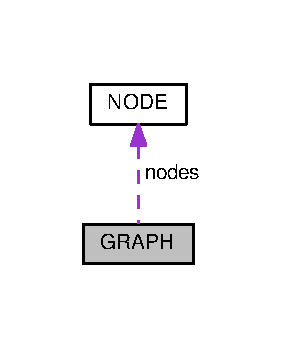
\includegraphics[width=137pt]{structGRAPH__coll__graph}
\end{center}
\end{figure}
\subsection*{Data Fields}
\begin{DoxyCompactItemize}
\item 
\hyperlink{structNODE}{N\+O\+DE} $\ast$$\ast$ \hyperlink{structGRAPH_adf5e0e2104ad2ebbafe01cd97d4a350d}{nodes}
\item 
uint32\+\_\+t \hyperlink{structGRAPH_aff09b6a0b0bb17a3565cb92bfdff8017}{num\+\_\+nodes}
\end{DoxyCompactItemize}


\subsection{Detailed Description}
This structure stores the necessary graph information. 

\subsection{Field Documentation}
\mbox{\Hypertarget{structGRAPH_adf5e0e2104ad2ebbafe01cd97d4a350d}\label{structGRAPH_adf5e0e2104ad2ebbafe01cd97d4a350d}} 
\index{G\+R\+A\+PH@{G\+R\+A\+PH}!nodes@{nodes}}
\index{nodes@{nodes}!G\+R\+A\+PH@{G\+R\+A\+PH}}
\subsubsection{\texorpdfstring{nodes}{nodes}}
{\footnotesize\ttfamily \hyperlink{structNODE}{N\+O\+DE}$\ast$$\ast$ G\+R\+A\+P\+H\+::nodes}

Array of pointers to nodes \mbox{\Hypertarget{structGRAPH_aff09b6a0b0bb17a3565cb92bfdff8017}\label{structGRAPH_aff09b6a0b0bb17a3565cb92bfdff8017}} 
\index{G\+R\+A\+PH@{G\+R\+A\+PH}!num\+\_\+nodes@{num\+\_\+nodes}}
\index{num\+\_\+nodes@{num\+\_\+nodes}!G\+R\+A\+PH@{G\+R\+A\+PH}}
\subsubsection{\texorpdfstring{num\+\_\+nodes}{num\_nodes}}
{\footnotesize\ttfamily uint32\+\_\+t G\+R\+A\+P\+H\+::num\+\_\+nodes}

Number of nodes in the graph (i.\+e length of the nodes array) 

The documentation for this struct was generated from the following file\+:\begin{DoxyCompactItemize}
\item 
headers/\hyperlink{graph_8h}{graph.\+h}\end{DoxyCompactItemize}

\hypertarget{structNODE}{}\section{N\+O\+DE Struct Reference}
\label{structNODE}\index{N\+O\+DE@{N\+O\+DE}}


This structure stores the information of a node of the graph.  




{\ttfamily \#include $<$node.\+h$>$}

\subsection*{Data Fields}
\begin{DoxyCompactItemize}
\item 
uint32\+\_\+t \hyperlink{structNODE_a5a4598006a4940d545ec4e8fda905826}{node\+\_\+id}
\item 
\hyperlink{edge_8h_ab4a642fc78a44ca8df119570b3288e13}{E\+D\+GE} $\ast$ \hyperlink{structNODE_ad3a6a918ba95f3ac9f897738ee2675e1}{adj\+\_\+list}
\item 
uint32\+\_\+t \hyperlink{structNODE_a34195e71189dd8b3b5d9988f0ad9416a}{num\+\_\+neighbors}
\item 
uint32\+\_\+t \hyperlink{structNODE_a0a2073821a4fe78d9700b75047328cd5}{degree}
\end{DoxyCompactItemize}


\subsection{Detailed Description}
This structure stores the information of a node of the graph. 

\subsection{Field Documentation}
\mbox{\Hypertarget{structNODE_ad3a6a918ba95f3ac9f897738ee2675e1}\label{structNODE_ad3a6a918ba95f3ac9f897738ee2675e1}} 
\index{N\+O\+DE@{N\+O\+DE}!adj\+\_\+list@{adj\+\_\+list}}
\index{adj\+\_\+list@{adj\+\_\+list}!N\+O\+DE@{N\+O\+DE}}
\subsubsection{\texorpdfstring{adj\+\_\+list}{adj\_list}}
{\footnotesize\ttfamily \hyperlink{edge_8h_ab4a642fc78a44ca8df119570b3288e13}{E\+D\+GE}$\ast$ N\+O\+D\+E\+::adj\+\_\+list}

Pointer to the adjacency list of the node \mbox{\Hypertarget{structNODE_a0a2073821a4fe78d9700b75047328cd5}\label{structNODE_a0a2073821a4fe78d9700b75047328cd5}} 
\index{N\+O\+DE@{N\+O\+DE}!degree@{degree}}
\index{degree@{degree}!N\+O\+DE@{N\+O\+DE}}
\subsubsection{\texorpdfstring{degree}{degree}}
{\footnotesize\ttfamily uint32\+\_\+t N\+O\+D\+E\+::degree}

The degree of the node \mbox{\Hypertarget{structNODE_a5a4598006a4940d545ec4e8fda905826}\label{structNODE_a5a4598006a4940d545ec4e8fda905826}} 
\index{N\+O\+DE@{N\+O\+DE}!node\+\_\+id@{node\+\_\+id}}
\index{node\+\_\+id@{node\+\_\+id}!N\+O\+DE@{N\+O\+DE}}
\subsubsection{\texorpdfstring{node\+\_\+id}{node\_id}}
{\footnotesize\ttfamily uint32\+\_\+t N\+O\+D\+E\+::node\+\_\+id}

The id of the node \mbox{\Hypertarget{structNODE_a34195e71189dd8b3b5d9988f0ad9416a}\label{structNODE_a34195e71189dd8b3b5d9988f0ad9416a}} 
\index{N\+O\+DE@{N\+O\+DE}!num\+\_\+neighbors@{num\+\_\+neighbors}}
\index{num\+\_\+neighbors@{num\+\_\+neighbors}!N\+O\+DE@{N\+O\+DE}}
\subsubsection{\texorpdfstring{num\+\_\+neighbors}{num\_neighbors}}
{\footnotesize\ttfamily uint32\+\_\+t N\+O\+D\+E\+::num\+\_\+neighbors}

The number of neighbors of the node (i.\+e the length of the adjacency list) 

The documentation for this struct was generated from the following file\+:\begin{DoxyCompactItemize}
\item 
headers/\hyperlink{node_8h}{node.\+h}\end{DoxyCompactItemize}

\hypertarget{structNODE__DEVICE}{}\section{N\+O\+D\+E\+\_\+\+D\+E\+V\+I\+CE Struct Reference}
\label{structNODE__DEVICE}\index{N\+O\+D\+E\+\_\+\+D\+E\+V\+I\+CE@{N\+O\+D\+E\+\_\+\+D\+E\+V\+I\+CE}}


This structure stores the information of a node within the graph. This structure is used in the kernel code and executed on the F\+P\+GA.  




{\ttfamily \#include $<$defs.\+h$>$}

\subsection*{Data Fields}
\begin{DoxyCompactItemize}
\item 
unsigned int \hyperlink{structNODE__DEVICE_ab0d37b3b13013ae6887a4fd809f7852e}{node\+\_\+id}
\item 
unsigned int \hyperlink{structNODE__DEVICE_af2adfd1f609392bfe1974b08b3080944}{first\+\_\+ind}
\item 
unsigned int \hyperlink{structNODE__DEVICE_aa13774c8a904d4696fd8e9c91fcc604c}{last\+\_\+ind}
\end{DoxyCompactItemize}


\subsection{Detailed Description}
This structure stores the information of a node within the graph. This structure is used in the kernel code and executed on the F\+P\+GA. 

\subsection{Field Documentation}
\mbox{\Hypertarget{structNODE__DEVICE_af2adfd1f609392bfe1974b08b3080944}\label{structNODE__DEVICE_af2adfd1f609392bfe1974b08b3080944}} 
\index{N\+O\+D\+E\+\_\+\+D\+E\+V\+I\+CE@{N\+O\+D\+E\+\_\+\+D\+E\+V\+I\+CE}!first\+\_\+ind@{first\+\_\+ind}}
\index{first\+\_\+ind@{first\+\_\+ind}!N\+O\+D\+E\+\_\+\+D\+E\+V\+I\+CE@{N\+O\+D\+E\+\_\+\+D\+E\+V\+I\+CE}}
\subsubsection{\texorpdfstring{first\+\_\+ind}{first\_ind}}
{\footnotesize\ttfamily unsigned int N\+O\+D\+E\+\_\+\+D\+E\+V\+I\+C\+E\+::first\+\_\+ind}

The index of the beginning of the edge subarray \mbox{\Hypertarget{structNODE__DEVICE_aa13774c8a904d4696fd8e9c91fcc604c}\label{structNODE__DEVICE_aa13774c8a904d4696fd8e9c91fcc604c}} 
\index{N\+O\+D\+E\+\_\+\+D\+E\+V\+I\+CE@{N\+O\+D\+E\+\_\+\+D\+E\+V\+I\+CE}!last\+\_\+ind@{last\+\_\+ind}}
\index{last\+\_\+ind@{last\+\_\+ind}!N\+O\+D\+E\+\_\+\+D\+E\+V\+I\+CE@{N\+O\+D\+E\+\_\+\+D\+E\+V\+I\+CE}}
\subsubsection{\texorpdfstring{last\+\_\+ind}{last\_ind}}
{\footnotesize\ttfamily unsigned int N\+O\+D\+E\+\_\+\+D\+E\+V\+I\+C\+E\+::last\+\_\+ind}

The index of the final of the edge subarray \mbox{\Hypertarget{structNODE__DEVICE_ab0d37b3b13013ae6887a4fd809f7852e}\label{structNODE__DEVICE_ab0d37b3b13013ae6887a4fd809f7852e}} 
\index{N\+O\+D\+E\+\_\+\+D\+E\+V\+I\+CE@{N\+O\+D\+E\+\_\+\+D\+E\+V\+I\+CE}!node\+\_\+id@{node\+\_\+id}}
\index{node\+\_\+id@{node\+\_\+id}!N\+O\+D\+E\+\_\+\+D\+E\+V\+I\+CE@{N\+O\+D\+E\+\_\+\+D\+E\+V\+I\+CE}}
\subsubsection{\texorpdfstring{node\+\_\+id}{node\_id}}
{\footnotesize\ttfamily unsigned int N\+O\+D\+E\+\_\+\+D\+E\+V\+I\+C\+E\+::node\+\_\+id}

The id of the node 

The documentation for this struct was generated from the following file\+:\begin{DoxyCompactItemize}
\item 
headers/\hyperlink{defs_8h}{defs.\+h}\end{DoxyCompactItemize}

\hypertarget{structTASK}{}\section{T\+A\+SK Struct Reference}
\label{structTASK}\index{T\+A\+SK@{T\+A\+SK}}


This structure contains the information of a pair of nodes (u,v). Each pair of nodes is processed by a different kernel instance on a S\+I\+MD manner This structure is used in the kernel code and executed on the F\+P\+GA.  




{\ttfamily \#include $<$defs.\+h$>$}



Collaboration diagram for T\+A\+SK\+:\nopagebreak
\begin{figure}[H]
\begin{center}
\leavevmode
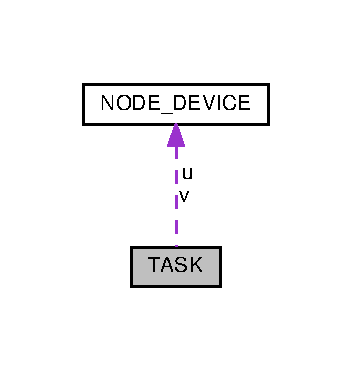
\includegraphics[width=169pt]{structTASK__coll__graph}
\end{center}
\end{figure}
\subsection*{Data Fields}
\begin{DoxyCompactItemize}
\item 
\hyperlink{structNODE__DEVICE}{N\+O\+D\+E\+\_\+\+D\+E\+V\+I\+CE} \hyperlink{structTASK_a40c47e76a10f508bc4757b4e79c65ef1}{u}
\item 
\hyperlink{structNODE__DEVICE}{N\+O\+D\+E\+\_\+\+D\+E\+V\+I\+CE} \hyperlink{structTASK_aa8bc9e3d0203b93cfc0dd927e3972fde}{v}
\end{DoxyCompactItemize}


\subsection{Detailed Description}
This structure contains the information of a pair of nodes (u,v). Each pair of nodes is processed by a different kernel instance on a S\+I\+MD manner This structure is used in the kernel code and executed on the F\+P\+GA. 

\subsection{Field Documentation}
\mbox{\Hypertarget{structTASK_a40c47e76a10f508bc4757b4e79c65ef1}\label{structTASK_a40c47e76a10f508bc4757b4e79c65ef1}} 
\index{T\+A\+SK@{T\+A\+SK}!u@{u}}
\index{u@{u}!T\+A\+SK@{T\+A\+SK}}
\subsubsection{\texorpdfstring{u}{u}}
{\footnotesize\ttfamily \hyperlink{structNODE__DEVICE}{N\+O\+D\+E\+\_\+\+D\+E\+V\+I\+CE} T\+A\+S\+K\+::u}

The first node of the pair that conforms the \hyperlink{structTASK}{T\+A\+SK} \mbox{\Hypertarget{structTASK_aa8bc9e3d0203b93cfc0dd927e3972fde}\label{structTASK_aa8bc9e3d0203b93cfc0dd927e3972fde}} 
\index{T\+A\+SK@{T\+A\+SK}!v@{v}}
\index{v@{v}!T\+A\+SK@{T\+A\+SK}}
\subsubsection{\texorpdfstring{v}{v}}
{\footnotesize\ttfamily \hyperlink{structNODE__DEVICE}{N\+O\+D\+E\+\_\+\+D\+E\+V\+I\+CE} T\+A\+S\+K\+::v}

The second node of the pair that conforms the \hyperlink{structTASK}{T\+A\+SK} 

The documentation for this struct was generated from the following file\+:\begin{DoxyCompactItemize}
\item 
headers/\hyperlink{defs_8h}{defs.\+h}\end{DoxyCompactItemize}

\chapter{File Documentation}
\hypertarget{aux_8h}{}\section{headers/aux.h File Reference}
\label{aux_8h}\index{headers/aux.\+h@{headers/aux.\+h}}


This file contains the definitions of some auxiliary functions~\newline
 used by the main program run the program.  


{\ttfamily \#include \char`\"{}../headers/triads.\+h\char`\"{}}\newline
{\ttfamily \#include $<$string.\+h$>$}\newline
Include dependency graph for aux.\+h\+:
\nopagebreak
\begin{figure}[H]
\begin{center}
\leavevmode
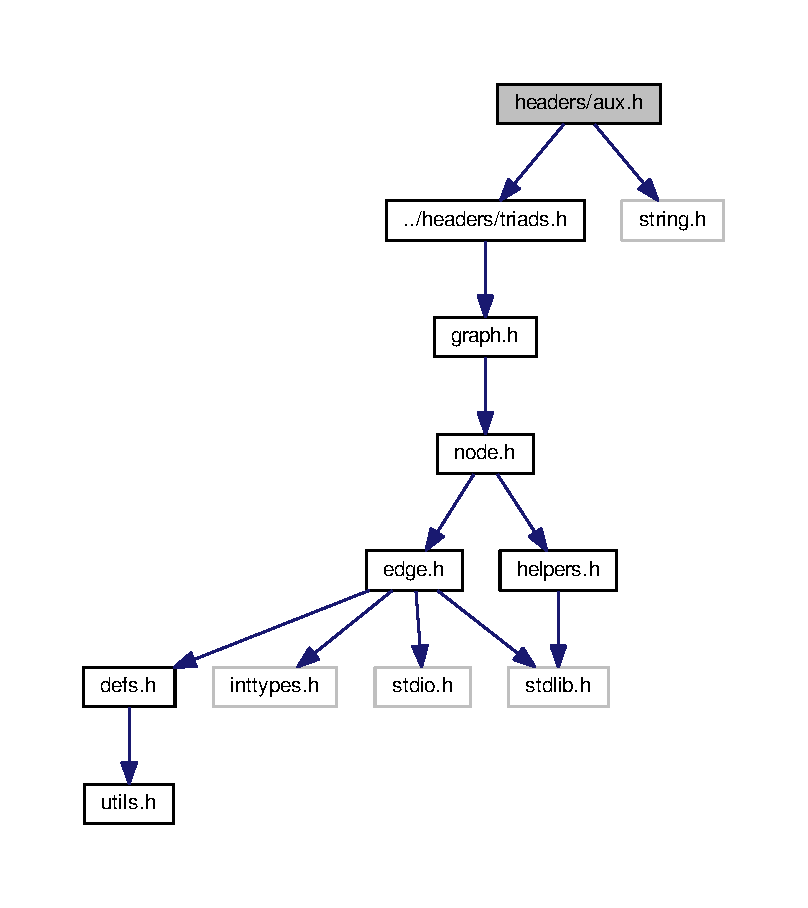
\includegraphics[width=350pt]{aux_8h__incl}
\end{center}
\end{figure}
This graph shows which files directly or indirectly include this file\+:
\nopagebreak
\begin{figure}[H]
\begin{center}
\leavevmode
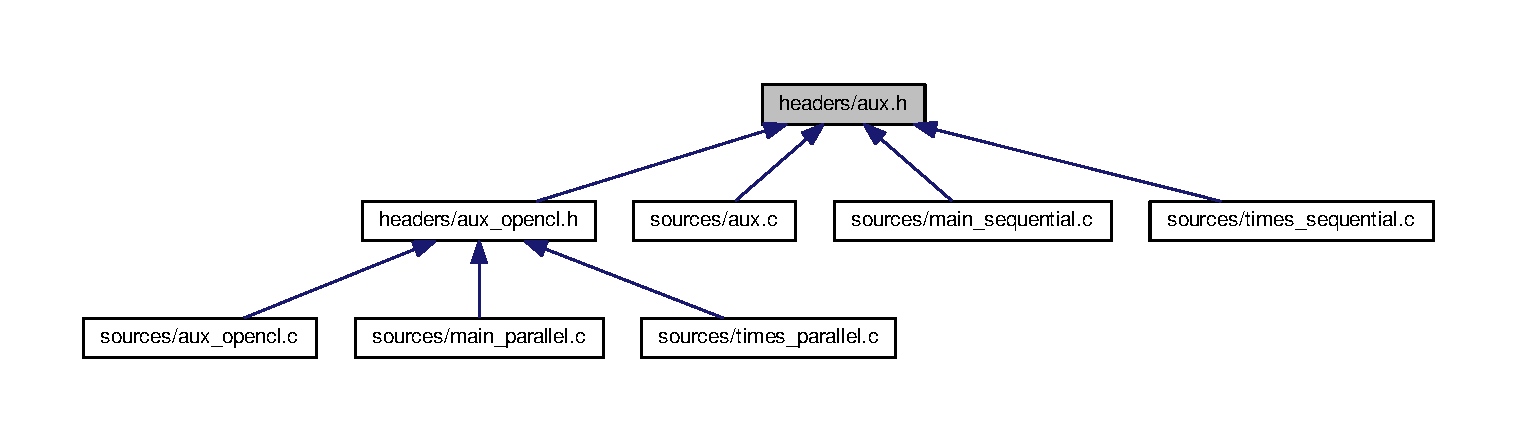
\includegraphics[width=350pt]{aux_8h__dep__incl}
\end{center}
\end{figure}
\subsection*{Functions}
\begin{DoxyCompactItemize}
\item 
void \hyperlink{aux_8h_a2d7f0126a191ecc47001de15e44eb4f9}{display\+\_\+graph\+\_\+summary} (\hyperlink{structGRAPH}{G\+R\+A\+PH} $\ast$g)
\begin{DoxyCompactList}\small\item\em Function that displays a summary of graph g printing its number of nodes, edges and triads. \end{DoxyCompactList}\item 
\hyperlink{utils_8h_a3e5b8192e7d9ffaf3542f1210aec18dd}{B\+O\+OL} \hyperlink{aux_8h_a2f5ae95e590fba7aaae015b750080579}{is\+\_\+ordered\+\_\+kernel} (char $\ast$name\+\_\+kernel)
\begin{DoxyCompactList}\small\item\em Function that checks the name of a kernel to discover if the kernel expects ordered input. \end{DoxyCompactList}\item 
\hyperlink{utils_8h_a3e5b8192e7d9ffaf3542f1210aec18dd}{B\+O\+OL} \hyperlink{aux_8h_abe467f2222de7b22db9f67f5ce6a529c}{is\+\_\+\+N\+D\+Range\+\_\+kernel} (char $\ast$name\+\_\+kernel)
\begin{DoxyCompactList}\small\item\em Function that checks the name of a kernel to discover if the kernel is a N\+D\+Range kernel. \end{DoxyCompactList}\item 
\hyperlink{utils_8h_a3e5b8192e7d9ffaf3542f1210aec18dd}{B\+O\+OL} \hyperlink{aux_8h_a1b1e4c6a6f5d3a0fc38e4c4cd17aa8e5}{is\+\_\+\+B\+M\+\_\+kernel} (char $\ast$name\+\_\+kernel)
\begin{DoxyCompactList}\small\item\em Function that checks the name of a kernel to discover if the kernel implements a BM algorithm. \end{DoxyCompactList}\item 
void \hyperlink{aux_8h_afc44cd39add4462b508953982dfa66b7}{write\+\_\+times} (char $\ast$times\+\_\+name, \hyperlink{structGRAPH}{G\+R\+A\+PH} $\ast$g, double reading\+\_\+time, double execution\+\_\+time)
\begin{DoxyCompactList}\small\item\em Function that writes performance data to a file. \end{DoxyCompactList}\item 
void \hyperlink{aux_8h_a3f18520902448cec9b1693f8914ca023}{rand\+\_\+graph\+\_\+generation} (unsigned int num\+\_\+nodes, unsigned int num\+\_\+edges, unsigned int seed, char $\ast$namefile)
\begin{DoxyCompactList}\small\item\em Function that randomly generates a graph and writes it to a file. \end{DoxyCompactList}\end{DoxyCompactItemize}


\subsection{Detailed Description}
This file contains the definitions of some auxiliary functions~\newline
 used by the main program run the program. 

\begin{DoxyAuthor}{Author}
\+: Carlos Alfaro
\end{DoxyAuthor}
\begin{DoxyDate}{Date}
\+: 18-\/12-\/2017 
\end{DoxyDate}


\subsection{Function Documentation}
\mbox{\Hypertarget{aux_8h_a2d7f0126a191ecc47001de15e44eb4f9}\label{aux_8h_a2d7f0126a191ecc47001de15e44eb4f9}} 
\index{aux.\+h@{aux.\+h}!display\+\_\+graph\+\_\+summary@{display\+\_\+graph\+\_\+summary}}
\index{display\+\_\+graph\+\_\+summary@{display\+\_\+graph\+\_\+summary}!aux.\+h@{aux.\+h}}
\subsubsection{\texorpdfstring{display\+\_\+graph\+\_\+summary()}{display\_graph\_summary()}}
{\footnotesize\ttfamily void display\+\_\+graph\+\_\+summary (\begin{DoxyParamCaption}\item[{\hyperlink{structGRAPH}{G\+R\+A\+PH} $\ast$}]{g }\end{DoxyParamCaption})}



Function that displays a summary of graph g printing its number of nodes, edges and triads. 


\begin{DoxyParams}{Parameters}
{\em G\+R\+A\+P\+H$\ast$} & g\+: The input graph.\\
\hline
\end{DoxyParams}
\begin{DoxyReturn}{Returns}
None 
\end{DoxyReturn}
\mbox{\Hypertarget{aux_8h_a1b1e4c6a6f5d3a0fc38e4c4cd17aa8e5}\label{aux_8h_a1b1e4c6a6f5d3a0fc38e4c4cd17aa8e5}} 
\index{aux.\+h@{aux.\+h}!is\+\_\+\+B\+M\+\_\+kernel@{is\+\_\+\+B\+M\+\_\+kernel}}
\index{is\+\_\+\+B\+M\+\_\+kernel@{is\+\_\+\+B\+M\+\_\+kernel}!aux.\+h@{aux.\+h}}
\subsubsection{\texorpdfstring{is\+\_\+\+B\+M\+\_\+kernel()}{is\_BM\_kernel()}}
{\footnotesize\ttfamily \hyperlink{utils_8h_a3e5b8192e7d9ffaf3542f1210aec18dd}{B\+O\+OL} is\+\_\+\+B\+M\+\_\+kernel (\begin{DoxyParamCaption}\item[{char $\ast$}]{name\+\_\+kernel }\end{DoxyParamCaption})}



Function that checks the name of a kernel to discover if the kernel implements a BM algorithm. 


\begin{DoxyParams}{Parameters}
{\em char$\ast$} & name\+\_\+kernel\+: The name of the kernel.\\
\hline
\end{DoxyParams}
\begin{DoxyReturn}{Returns}
B\+O\+OL\+: T\+R\+UE if the kernel implements BM.~\newline
 F\+A\+L\+SE otherwise 
\end{DoxyReturn}
\mbox{\Hypertarget{aux_8h_abe467f2222de7b22db9f67f5ce6a529c}\label{aux_8h_abe467f2222de7b22db9f67f5ce6a529c}} 
\index{aux.\+h@{aux.\+h}!is\+\_\+\+N\+D\+Range\+\_\+kernel@{is\+\_\+\+N\+D\+Range\+\_\+kernel}}
\index{is\+\_\+\+N\+D\+Range\+\_\+kernel@{is\+\_\+\+N\+D\+Range\+\_\+kernel}!aux.\+h@{aux.\+h}}
\subsubsection{\texorpdfstring{is\+\_\+\+N\+D\+Range\+\_\+kernel()}{is\_NDRange\_kernel()}}
{\footnotesize\ttfamily \hyperlink{utils_8h_a3e5b8192e7d9ffaf3542f1210aec18dd}{B\+O\+OL} is\+\_\+\+N\+D\+Range\+\_\+kernel (\begin{DoxyParamCaption}\item[{char $\ast$}]{name\+\_\+kernel }\end{DoxyParamCaption})}



Function that checks the name of a kernel to discover if the kernel is a N\+D\+Range kernel. 


\begin{DoxyParams}{Parameters}
{\em char$\ast$} & name\+\_\+kernel\+: The name of the kernel.\\
\hline
\end{DoxyParams}
\begin{DoxyReturn}{Returns}
B\+O\+OL\+: T\+R\+UE if it is a N\+D\+Range kernel.~\newline
 F\+A\+L\+SE otherwise 
\end{DoxyReturn}
\mbox{\Hypertarget{aux_8h_a2f5ae95e590fba7aaae015b750080579}\label{aux_8h_a2f5ae95e590fba7aaae015b750080579}} 
\index{aux.\+h@{aux.\+h}!is\+\_\+ordered\+\_\+kernel@{is\+\_\+ordered\+\_\+kernel}}
\index{is\+\_\+ordered\+\_\+kernel@{is\+\_\+ordered\+\_\+kernel}!aux.\+h@{aux.\+h}}
\subsubsection{\texorpdfstring{is\+\_\+ordered\+\_\+kernel()}{is\_ordered\_kernel()}}
{\footnotesize\ttfamily \hyperlink{utils_8h_a3e5b8192e7d9ffaf3542f1210aec18dd}{B\+O\+OL} is\+\_\+ordered\+\_\+kernel (\begin{DoxyParamCaption}\item[{char $\ast$}]{name\+\_\+kernel }\end{DoxyParamCaption})}



Function that checks the name of a kernel to discover if the kernel expects ordered input. 


\begin{DoxyParams}{Parameters}
{\em char$\ast$} & name\+\_\+kernel\+: The name of the kernel.\\
\hline
\end{DoxyParams}
\begin{DoxyReturn}{Returns}
B\+O\+OL\+: T\+R\+UE if the kernel expects ordered input.~\newline
 F\+A\+L\+SE otherwise 
\end{DoxyReturn}
\mbox{\Hypertarget{aux_8h_a3f18520902448cec9b1693f8914ca023}\label{aux_8h_a3f18520902448cec9b1693f8914ca023}} 
\index{aux.\+h@{aux.\+h}!rand\+\_\+graph\+\_\+generation@{rand\+\_\+graph\+\_\+generation}}
\index{rand\+\_\+graph\+\_\+generation@{rand\+\_\+graph\+\_\+generation}!aux.\+h@{aux.\+h}}
\subsubsection{\texorpdfstring{rand\+\_\+graph\+\_\+generation()}{rand\_graph\_generation()}}
{\footnotesize\ttfamily void rand\+\_\+graph\+\_\+generation (\begin{DoxyParamCaption}\item[{unsigned int}]{num\+\_\+nodes,  }\item[{unsigned int}]{num\+\_\+edges,  }\item[{unsigned int}]{seed,  }\item[{char $\ast$}]{namefile }\end{DoxyParamCaption})}



Function that randomly generates a graph and writes it to a file. 


\begin{DoxyParams}{Parameters}
{\em unsigned} & int num\+\_\+nodes\+: Number of nodes desired. \\
\hline
{\em unsigned} & int num\+\_\+edges\+: Number of edges desired. \\
\hline
{\em unsigned} & int seed\+: The seed for rand() function \\
\hline
{\em char$\ast$} & namefile\+: The name of the file in which to write the graph.\\
\hline
\end{DoxyParams}
\begin{DoxyReturn}{Returns}
None 
\end{DoxyReturn}
\mbox{\Hypertarget{aux_8h_afc44cd39add4462b508953982dfa66b7}\label{aux_8h_afc44cd39add4462b508953982dfa66b7}} 
\index{aux.\+h@{aux.\+h}!write\+\_\+times@{write\+\_\+times}}
\index{write\+\_\+times@{write\+\_\+times}!aux.\+h@{aux.\+h}}
\subsubsection{\texorpdfstring{write\+\_\+times()}{write\_times()}}
{\footnotesize\ttfamily void write\+\_\+times (\begin{DoxyParamCaption}\item[{char $\ast$}]{times\+\_\+name,  }\item[{\hyperlink{structGRAPH}{G\+R\+A\+PH} $\ast$}]{g,  }\item[{double}]{reading\+\_\+time,  }\item[{double}]{execution\+\_\+time }\end{DoxyParamCaption})}



Function that writes performance data to a file. 


\begin{DoxyParams}{Parameters}
{\em char$\ast$} & times\+\_\+name\+: The name of the file in which to write the results. \\
\hline
{\em G\+R\+A\+P\+H$\ast$} & g\+: The graph under analysis. \\
\hline
{\em double} & reading\+\_\+time\+: Graph reading time. \\
\hline
{\em double} & execution time\+: Triad census execution time.\\
\hline
\end{DoxyParams}
\begin{DoxyReturn}{Returns}
None 
\end{DoxyReturn}

\hypertarget{aux__opencl_8h}{}\section{headers/aux\+\_\+opencl.h File Reference}
\label{aux__opencl_8h}\index{headers/aux\+\_\+opencl.\+h@{headers/aux\+\_\+opencl.\+h}}


This file contains the definitions of the auxiliary functions~\newline
 used by the main program run the Open\+CL application. It includes functions~\newline
 to create the objects necessary to execute the application.  


{\ttfamily \#include \char`\"{}C\+L/opencl.\+h\char`\"{}}\newline
{\ttfamily \#include \char`\"{}aux.\+h\char`\"{}}\newline
Include dependency graph for aux\+\_\+opencl.\+h\+:
\nopagebreak
\begin{figure}[H]
\begin{center}
\leavevmode
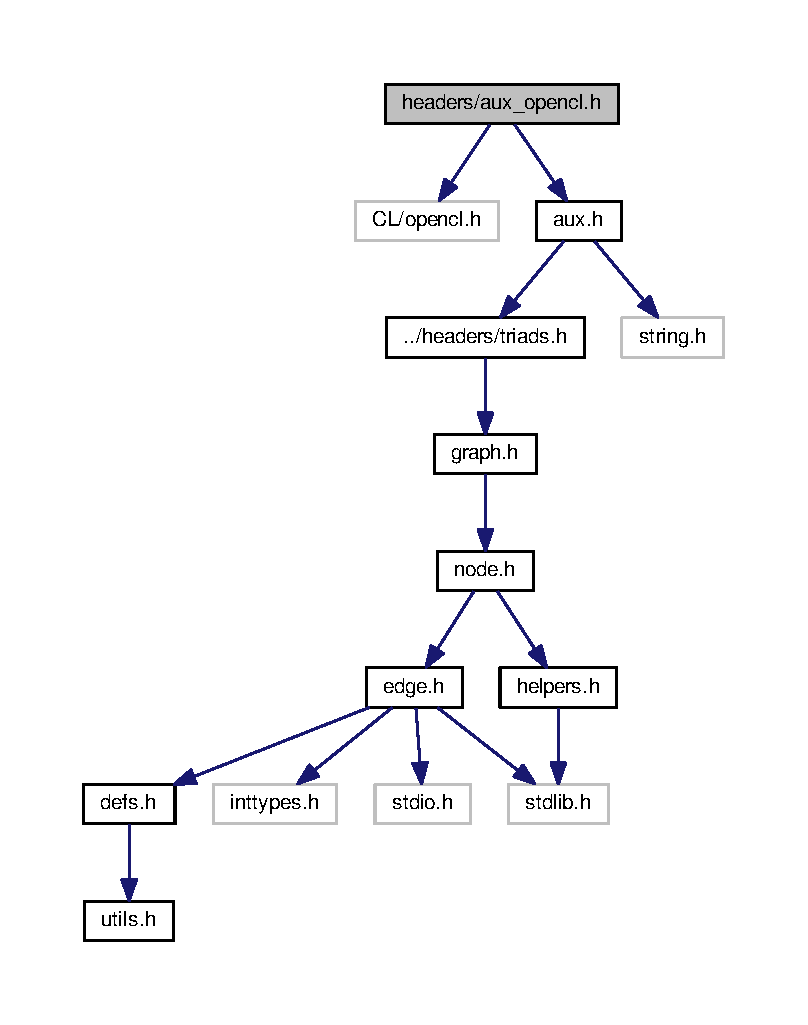
\includegraphics[width=350pt]{aux__opencl_8h__incl}
\end{center}
\end{figure}
This graph shows which files directly or indirectly include this file\+:
\nopagebreak
\begin{figure}[H]
\begin{center}
\leavevmode
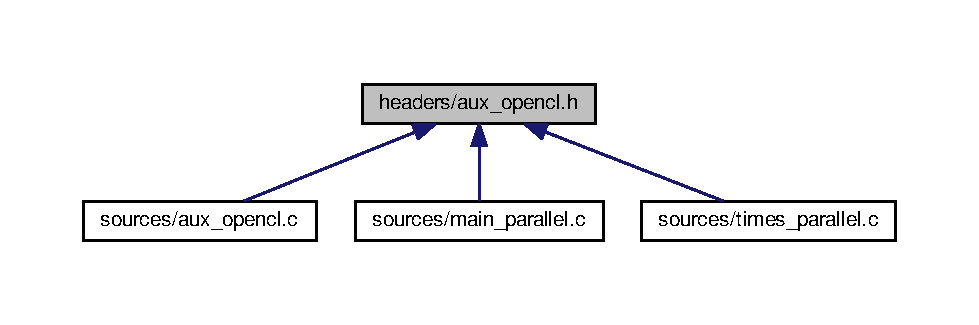
\includegraphics[width=350pt]{aux__opencl_8h__dep__incl}
\end{center}
\end{figure}
\subsection*{Macros}
\begin{DoxyCompactItemize}
\item 
\mbox{\Hypertarget{aux__opencl_8h_a82acb32225c05e9aa4c524c40bc5852a}\label{aux__opencl_8h_a82acb32225c05e9aa4c524c40bc5852a}} 
\#define {\bfseries M\+A\+X\+\_\+\+C\+H\+AR}~256
\item 
\mbox{\Hypertarget{aux__opencl_8h_a062369491b5189e53dfdd8e1229a8ece}\label{aux__opencl_8h_a062369491b5189e53dfdd8e1229a8ece}} 
\#define {\bfseries S\+T\+R\+I\+N\+G\+\_\+\+B\+U\+F\+F\+E\+R\+\_\+\+L\+EN}~1024
\end{DoxyCompactItemize}
\subsection*{Functions}
\begin{DoxyCompactItemize}
\item 
void \hyperlink{aux__opencl_8h_ae9b40ed1990a1e4162a6b6c4fe8419a5}{setup} (cl\+\_\+platform\+\_\+id $\ast$platform, cl\+\_\+device\+\_\+id $\ast$device, cl\+\_\+context $\ast$context)
\begin{DoxyCompactList}\small\item\em Function sets up the proper Open\+CL environment for creating and executing kernels.~\newline
This process involves selecting an Open\+CL platform and an attached device, as well as creating an execution context. \end{DoxyCompactList}\item 
cl\+\_\+program \hyperlink{aux__opencl_8h_a335b0aeeb63d503ee152a3adc84ab19e}{create\+\_\+build\+\_\+program} (char $\ast$filename, cl\+\_\+context context, cl\+\_\+device\+\_\+id $\ast$device)
\begin{DoxyCompactList}\small\item\em Function creates and builds the program from a binary .aocx file~\newline
This process involves selecting an Open\+CL platform and an attached device, as well as creating an execution context. \end{DoxyCompactList}\item 
void \hyperlink{aux__opencl_8h_a8e2f457f73112edd95ab085f5de0d4bd}{display\+\_\+platform\+\_\+info} (cl\+\_\+platform\+\_\+id platform)
\begin{DoxyCompactList}\small\item\em Function displays information about the Open\+CL platform. \end{DoxyCompactList}\item 
void \hyperlink{aux__opencl_8h_ab9ec1cbdd471182d6d645cb348ddcfa0}{display\+\_\+device\+\_\+info} (cl\+\_\+device\+\_\+id device)
\begin{DoxyCompactList}\small\item\em Function displays information about the Open\+CL device used. \end{DoxyCompactList}\item 
void \hyperlink{aux__opencl_8h_a2e23d888af16d40462205572135139a4}{check\+\_\+error} (cl\+\_\+int error\+\_\+code, const char $\ast$message)
\begin{DoxyCompactList}\small\item\em Function checks the error code returned by a A\+PI function. If there has been~\newline
an error, displays the errror code and stops execution. \end{DoxyCompactList}\item 
cl\+\_\+mem \hyperlink{aux__opencl_8h_a611ba60155d74de941fd81b533d28c1a}{create\+\_\+and\+\_\+write\+\_\+buffer} (cl\+\_\+context context, cl\+\_\+command\+\_\+queue queue, size\+\_\+t size, void $\ast$host\+\_\+ptr)
\begin{DoxyCompactList}\small\item\em Function that creates an Open\+CL buffer object and fills it with certain information. \end{DoxyCompactList}\item 
void \hyperlink{aux__opencl_8h_afefd6c0004b4a7972a5f55cb8f386211}{set\+\_\+args} (cl\+\_\+kernel kernel, void $\ast$arg0, void $\ast$arg1, void $\ast$arg2, void $\ast$arg3)
\begin{DoxyCompactList}\small\item\em Function that sets the four argument of an Open\+CL kernel. \end{DoxyCompactList}\end{DoxyCompactItemize}


\subsection{Detailed Description}
This file contains the definitions of the auxiliary functions~\newline
 used by the main program run the Open\+CL application. It includes functions~\newline
 to create the objects necessary to execute the application. 

\begin{DoxyAuthor}{Author}
\+: Carlos Alfaro
\end{DoxyAuthor}
\begin{DoxyDate}{Date}
\+: 18-\/12-\/2017 
\end{DoxyDate}


\subsection{Function Documentation}
\mbox{\Hypertarget{aux__opencl_8h_a2e23d888af16d40462205572135139a4}\label{aux__opencl_8h_a2e23d888af16d40462205572135139a4}} 
\index{aux\+\_\+opencl.\+h@{aux\+\_\+opencl.\+h}!check\+\_\+error@{check\+\_\+error}}
\index{check\+\_\+error@{check\+\_\+error}!aux\+\_\+opencl.\+h@{aux\+\_\+opencl.\+h}}
\subsubsection{\texorpdfstring{check\+\_\+error()}{check\_error()}}
{\footnotesize\ttfamily void check\+\_\+error (\begin{DoxyParamCaption}\item[{cl\+\_\+int}]{error\+\_\+code,  }\item[{const char $\ast$}]{message }\end{DoxyParamCaption})}



Function checks the error code returned by a A\+PI function. If there has been~\newline
an error, displays the errror code and stops execution. 


\begin{DoxyParams}{Parameters}
{\em cl\+\_\+int} & error\+\_\+code\+: error code returned by the function \\
\hline
{\em const} & char$\ast$ message\+: Message to be printed\\
\hline
\end{DoxyParams}
\begin{DoxyReturn}{Returns}
None 
\end{DoxyReturn}
\mbox{\Hypertarget{aux__opencl_8h_a611ba60155d74de941fd81b533d28c1a}\label{aux__opencl_8h_a611ba60155d74de941fd81b533d28c1a}} 
\index{aux\+\_\+opencl.\+h@{aux\+\_\+opencl.\+h}!create\+\_\+and\+\_\+write\+\_\+buffer@{create\+\_\+and\+\_\+write\+\_\+buffer}}
\index{create\+\_\+and\+\_\+write\+\_\+buffer@{create\+\_\+and\+\_\+write\+\_\+buffer}!aux\+\_\+opencl.\+h@{aux\+\_\+opencl.\+h}}
\subsubsection{\texorpdfstring{create\+\_\+and\+\_\+write\+\_\+buffer()}{create\_and\_write\_buffer()}}
{\footnotesize\ttfamily cl\+\_\+mem create\+\_\+and\+\_\+write\+\_\+buffer (\begin{DoxyParamCaption}\item[{cl\+\_\+context}]{context,  }\item[{cl\+\_\+command\+\_\+queue}]{queue,  }\item[{size\+\_\+t}]{size,  }\item[{void $\ast$}]{host\+\_\+ptr }\end{DoxyParamCaption})}



Function that creates an Open\+CL buffer object and fills it with certain information. 


\begin{DoxyParams}{Parameters}
{\em cl\+\_\+context} & context\+: Open\+CL context \\
\hline
{\em cl\+\_\+command\+\_\+queue} & queue\+: Open\+CL queue for the communication between host and Open\+CL device \\
\hline
{\em size\+\_\+t} & size\+: Size in bytes of the buffer \\
\hline
{\em void$\ast$} & host\+\_\+ptr\+: Pointer to the data to be copied in the newly created buffer.\\
\hline
\end{DoxyParams}
\begin{DoxyReturn}{Returns}
cl\+\_\+mem The buffer created. 
\end{DoxyReturn}
\mbox{\Hypertarget{aux__opencl_8h_a335b0aeeb63d503ee152a3adc84ab19e}\label{aux__opencl_8h_a335b0aeeb63d503ee152a3adc84ab19e}} 
\index{aux\+\_\+opencl.\+h@{aux\+\_\+opencl.\+h}!create\+\_\+build\+\_\+program@{create\+\_\+build\+\_\+program}}
\index{create\+\_\+build\+\_\+program@{create\+\_\+build\+\_\+program}!aux\+\_\+opencl.\+h@{aux\+\_\+opencl.\+h}}
\subsubsection{\texorpdfstring{create\+\_\+build\+\_\+program()}{create\_build\_program()}}
{\footnotesize\ttfamily cl\+\_\+program create\+\_\+build\+\_\+program (\begin{DoxyParamCaption}\item[{char $\ast$}]{filename,  }\item[{cl\+\_\+context}]{context,  }\item[{cl\+\_\+device\+\_\+id $\ast$}]{device }\end{DoxyParamCaption})}



Function creates and builds the program from a binary .aocx file~\newline
This process involves selecting an Open\+CL platform and an attached device, as well as creating an execution context. 


\begin{DoxyParams}{Parameters}
{\em char} & $\ast$filename\+: Name of the .aocx file containing the binary H\+DL file \\
\hline
{\em cl\+\_\+context} & context\+: Open\+CL context \\
\hline
{\em cl\+\_\+device\+\_\+id$\ast$} & device\+: Pointer to the Open\+CL device id\\
\hline
\end{DoxyParams}
\begin{DoxyReturn}{Returns}
None 
\end{DoxyReturn}
\mbox{\Hypertarget{aux__opencl_8h_ab9ec1cbdd471182d6d645cb348ddcfa0}\label{aux__opencl_8h_ab9ec1cbdd471182d6d645cb348ddcfa0}} 
\index{aux\+\_\+opencl.\+h@{aux\+\_\+opencl.\+h}!display\+\_\+device\+\_\+info@{display\+\_\+device\+\_\+info}}
\index{display\+\_\+device\+\_\+info@{display\+\_\+device\+\_\+info}!aux\+\_\+opencl.\+h@{aux\+\_\+opencl.\+h}}
\subsubsection{\texorpdfstring{display\+\_\+device\+\_\+info()}{display\_device\_info()}}
{\footnotesize\ttfamily void display\+\_\+device\+\_\+info (\begin{DoxyParamCaption}\item[{cl\+\_\+device\+\_\+id}]{device }\end{DoxyParamCaption})}



Function displays information about the Open\+CL device used. 


\begin{DoxyParams}{Parameters}
{\em cl\+\_\+device\+\_\+id} & device\+: Open\+CL device\\
\hline
\end{DoxyParams}
\begin{DoxyReturn}{Returns}
None 
\end{DoxyReturn}
\mbox{\Hypertarget{aux__opencl_8h_a8e2f457f73112edd95ab085f5de0d4bd}\label{aux__opencl_8h_a8e2f457f73112edd95ab085f5de0d4bd}} 
\index{aux\+\_\+opencl.\+h@{aux\+\_\+opencl.\+h}!display\+\_\+platform\+\_\+info@{display\+\_\+platform\+\_\+info}}
\index{display\+\_\+platform\+\_\+info@{display\+\_\+platform\+\_\+info}!aux\+\_\+opencl.\+h@{aux\+\_\+opencl.\+h}}
\subsubsection{\texorpdfstring{display\+\_\+platform\+\_\+info()}{display\_platform\_info()}}
{\footnotesize\ttfamily void display\+\_\+platform\+\_\+info (\begin{DoxyParamCaption}\item[{cl\+\_\+platform\+\_\+id}]{platform }\end{DoxyParamCaption})}



Function displays information about the Open\+CL platform. 


\begin{DoxyParams}{Parameters}
{\em cl\+\_\+platform\+\_\+id} & platform\+: Open\+CL platform\\
\hline
\end{DoxyParams}
\begin{DoxyReturn}{Returns}
None 
\end{DoxyReturn}
\mbox{\Hypertarget{aux__opencl_8h_afefd6c0004b4a7972a5f55cb8f386211}\label{aux__opencl_8h_afefd6c0004b4a7972a5f55cb8f386211}} 
\index{aux\+\_\+opencl.\+h@{aux\+\_\+opencl.\+h}!set\+\_\+args@{set\+\_\+args}}
\index{set\+\_\+args@{set\+\_\+args}!aux\+\_\+opencl.\+h@{aux\+\_\+opencl.\+h}}
\subsubsection{\texorpdfstring{set\+\_\+args()}{set\_args()}}
{\footnotesize\ttfamily void set\+\_\+args (\begin{DoxyParamCaption}\item[{cl\+\_\+kernel}]{kernel,  }\item[{void $\ast$}]{arg0,  }\item[{void $\ast$}]{arg1,  }\item[{void $\ast$}]{arg2,  }\item[{void $\ast$}]{arg3 }\end{DoxyParamCaption})}



Function that sets the four argument of an Open\+CL kernel. 


\begin{DoxyParams}{Parameters}
{\em cl\+\_\+kernel} & kernel\+: The kernel we want to set the params to \\
\hline
{\em void$\ast$} & arg0\+: First argument \\
\hline
{\em void$\ast$} & arg1\+: Seconde argument \\
\hline
{\em void$\ast$} & arg2\+: Third argument \\
\hline
{\em void$\ast$} & arg3\+: Fourth argument\\
\hline
\end{DoxyParams}
\begin{DoxyReturn}{Returns}
None 
\end{DoxyReturn}
\mbox{\Hypertarget{aux__opencl_8h_ae9b40ed1990a1e4162a6b6c4fe8419a5}\label{aux__opencl_8h_ae9b40ed1990a1e4162a6b6c4fe8419a5}} 
\index{aux\+\_\+opencl.\+h@{aux\+\_\+opencl.\+h}!setup@{setup}}
\index{setup@{setup}!aux\+\_\+opencl.\+h@{aux\+\_\+opencl.\+h}}
\subsubsection{\texorpdfstring{setup()}{setup()}}
{\footnotesize\ttfamily void setup (\begin{DoxyParamCaption}\item[{cl\+\_\+platform\+\_\+id $\ast$}]{platform,  }\item[{cl\+\_\+device\+\_\+id $\ast$}]{device,  }\item[{cl\+\_\+context $\ast$}]{context }\end{DoxyParamCaption})}



Function sets up the proper Open\+CL environment for creating and executing kernels.~\newline
This process involves selecting an Open\+CL platform and an attached device, as well as creating an execution context. 


\begin{DoxyParams}{Parameters}
{\em cl\+\_\+platform\+\_\+id$\ast$} & platform\+: Pointer to the Open\+CL platform (to be filled by the function) \\
\hline
{\em cl\+\_\+device\+\_\+id$\ast$} & device\+: Pointer to the Open\+CL device id (to be filled by the function) \\
\hline
{\em cl\+\_\+context$\ast$} & context\+: Pointer to the Open\+CL context (to be created by the function)\\
\hline
\end{DoxyParams}
\begin{DoxyReturn}{Returns}
None 
\end{DoxyReturn}

\hypertarget{BF__header_8h}{}\section{headers/\+B\+F\+\_\+header.h File Reference}
\label{BF__header_8h}\index{headers/\+B\+F\+\_\+header.\+h@{headers/\+B\+F\+\_\+header.\+h}}


This file contains the definitions of the functions needed to execute the Brute Force kernels.  


{\ttfamily \#include \char`\"{}defs.\+h\char`\"{}}\newline
Include dependency graph for B\+F\+\_\+header.\+h\+:
\nopagebreak
\begin{figure}[H]
\begin{center}
\leavevmode
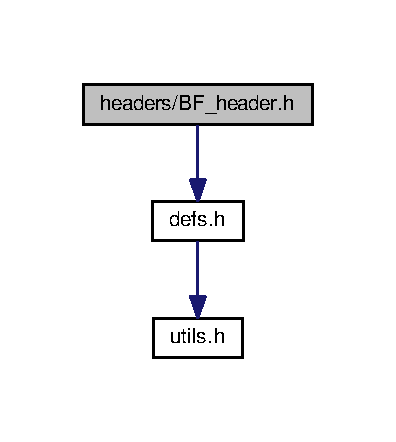
\includegraphics[width=190pt]{BF__header_8h__incl}
\end{center}
\end{figure}
\subsection*{Functions}
\begin{DoxyCompactItemize}
\item 
\mbox{\Hypertarget{BF__header_8h_a69417949e991b0a7b1e8f2a1f13c4dc0}\label{BF__header_8h_a69417949e991b0a7b1e8f2a1f13c4dc0}} 
short {\bfseries iso\+Tricode} (\+\_\+\+\_\+constant \hyperlink{structEDGE__DEVICE}{E\+D\+G\+E\+\_\+\+D\+E\+V\+I\+CE} $\ast$edges, \+\_\+\+\_\+constant \hyperlink{structNODE__DEVICE}{N\+O\+D\+E\+\_\+\+D\+E\+V\+I\+CE} $\ast$u, \+\_\+\+\_\+constant \hyperlink{structNODE__DEVICE}{N\+O\+D\+E\+\_\+\+D\+E\+V\+I\+CE} $\ast$v, \+\_\+\+\_\+constant \hyperlink{structNODE__DEVICE}{N\+O\+D\+E\+\_\+\+D\+E\+V\+I\+CE} $\ast$w)
\item 
\mbox{\Hypertarget{BF__header_8h_a95e0a6a9cc2e8a80b278084f31f027a3}\label{BF__header_8h_a95e0a6a9cc2e8a80b278084f31f027a3}} 
unsigned int {\bfseries get\+\_\+neighbor\+\_\+id} (\hyperlink{structEDGE__DEVICE}{E\+D\+G\+E\+\_\+\+D\+E\+V\+I\+CE} e)
\item 
\mbox{\Hypertarget{BF__header_8h_a3c6ec02b4ab708a4c4cc9d75d8b8bd3d}\label{BF__header_8h_a3c6ec02b4ab708a4c4cc9d75d8b8bd3d}} 
\hyperlink{utils_8h_aa268a41a13430b18e933ed40207178d0}{D\+I\+R\+E\+C\+T\+I\+ON} {\bfseries get\+\_\+direction} (\hyperlink{structEDGE__DEVICE}{E\+D\+G\+E\+\_\+\+D\+E\+V\+I\+CE} e)
\item 
\mbox{\Hypertarget{BF__header_8h_a74cf1e49f7fc6430637462ee91af3336}\label{BF__header_8h_a74cf1e49f7fc6430637462ee91af3336}} 
int {\bfseries linear\+\_\+search\+\_\+adj\+\_\+list} (\+\_\+\+\_\+constant \hyperlink{structEDGE__DEVICE}{E\+D\+G\+E\+\_\+\+D\+E\+V\+I\+CE} $\ast$table, unsigned int key, unsigned int first, unsigned int last)
\item 
\mbox{\Hypertarget{BF__header_8h_a0de6df960ecbc500aeb43bb72bbe3d24}\label{BF__header_8h_a0de6df960ecbc500aeb43bb72bbe3d24}} 
int {\bfseries binary\+\_\+search\+\_\+adj\+\_\+list} (\+\_\+\+\_\+constant \hyperlink{structEDGE__DEVICE}{E\+D\+G\+E\+\_\+\+D\+E\+V\+I\+CE} $\ast$table, unsigned int key, int first, int last)
\item 
\mbox{\Hypertarget{BF__header_8h_a34370d41d892802b47e65a79f8a5bed5}\label{BF__header_8h_a34370d41d892802b47e65a79f8a5bed5}} 
unsigned int {\bfseries get\+\_\+node\+\_\+id} (\+\_\+\+\_\+constant \hyperlink{structNODE__DEVICE}{N\+O\+D\+E\+\_\+\+D\+E\+V\+I\+CE} $\ast$n)
\item 
\mbox{\Hypertarget{BF__header_8h_a8b554f428904c83d3b6e49e66482dcb5}\label{BF__header_8h_a8b554f428904c83d3b6e49e66482dcb5}} 
int {\bfseries get\+\_\+neighbor\+\_\+pos} (\+\_\+\+\_\+constant \hyperlink{structEDGE__DEVICE}{E\+D\+G\+E\+\_\+\+D\+E\+V\+I\+CE} $\ast$edges, \+\_\+\+\_\+constant \hyperlink{structNODE__DEVICE}{N\+O\+D\+E\+\_\+\+D\+E\+V\+I\+CE} $\ast$n, unsigned int nid)
\item 
\mbox{\Hypertarget{BF__header_8h_a32f3454ed00140c7181d15bb8619cf75}\label{BF__header_8h_a32f3454ed00140c7181d15bb8619cf75}} 
\hyperlink{utils_8h_a3e5b8192e7d9ffaf3542f1210aec18dd}{B\+O\+OL} {\bfseries not\+\_\+connected} (\+\_\+\+\_\+constant \hyperlink{structEDGE__DEVICE}{E\+D\+G\+E\+\_\+\+D\+E\+V\+I\+CE} $\ast$edges, \+\_\+\+\_\+constant \hyperlink{structNODE__DEVICE}{N\+O\+D\+E\+\_\+\+D\+E\+V\+I\+CE} $\ast$u, \+\_\+\+\_\+constant \hyperlink{structNODE__DEVICE}{N\+O\+D\+E\+\_\+\+D\+E\+V\+I\+CE} $\ast$v)
\item 
\mbox{\Hypertarget{BF__header_8h_a61a7d10a5e18fd084e19ffeb9e6ec1c7}\label{BF__header_8h_a61a7d10a5e18fd084e19ffeb9e6ec1c7}} 
\hyperlink{utils_8h_aa268a41a13430b18e933ed40207178d0}{D\+I\+R\+E\+C\+T\+I\+ON} {\bfseries get\+\_\+dir\+\_\+between\+\_\+nodes} (\+\_\+\+\_\+constant \hyperlink{structEDGE__DEVICE}{E\+D\+G\+E\+\_\+\+D\+E\+V\+I\+CE} $\ast$edges, \+\_\+\+\_\+constant \hyperlink{structNODE__DEVICE}{N\+O\+D\+E\+\_\+\+D\+E\+V\+I\+CE} $\ast$u, \+\_\+\+\_\+constant \hyperlink{structNODE__DEVICE}{N\+O\+D\+E\+\_\+\+D\+E\+V\+I\+CE} $\ast$v)
\end{DoxyCompactItemize}


\subsection{Detailed Description}
This file contains the definitions of the functions needed to execute the Brute Force kernels. 

\begin{DoxyAuthor}{Author}
\+: Carlos Alfaro
\end{DoxyAuthor}
\begin{DoxyDate}{Date}
\+: 17-\/12-\/2017 
\end{DoxyDate}

\hypertarget{defs_8h}{}\section{headers/defs.h File Reference}
\label{defs_8h}\index{headers/defs.\+h@{headers/defs.\+h}}


This file contains the definitions of the structures that are used for the kernel code.  


{\ttfamily \#include \char`\"{}utils.\+h\char`\"{}}\newline
Include dependency graph for defs.\+h\+:\nopagebreak
\begin{figure}[H]
\begin{center}
\leavevmode
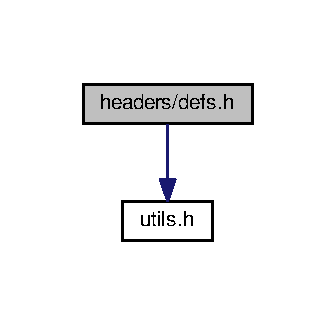
\includegraphics[width=161pt]{defs_8h__incl}
\end{center}
\end{figure}
This graph shows which files directly or indirectly include this file\+:
\nopagebreak
\begin{figure}[H]
\begin{center}
\leavevmode
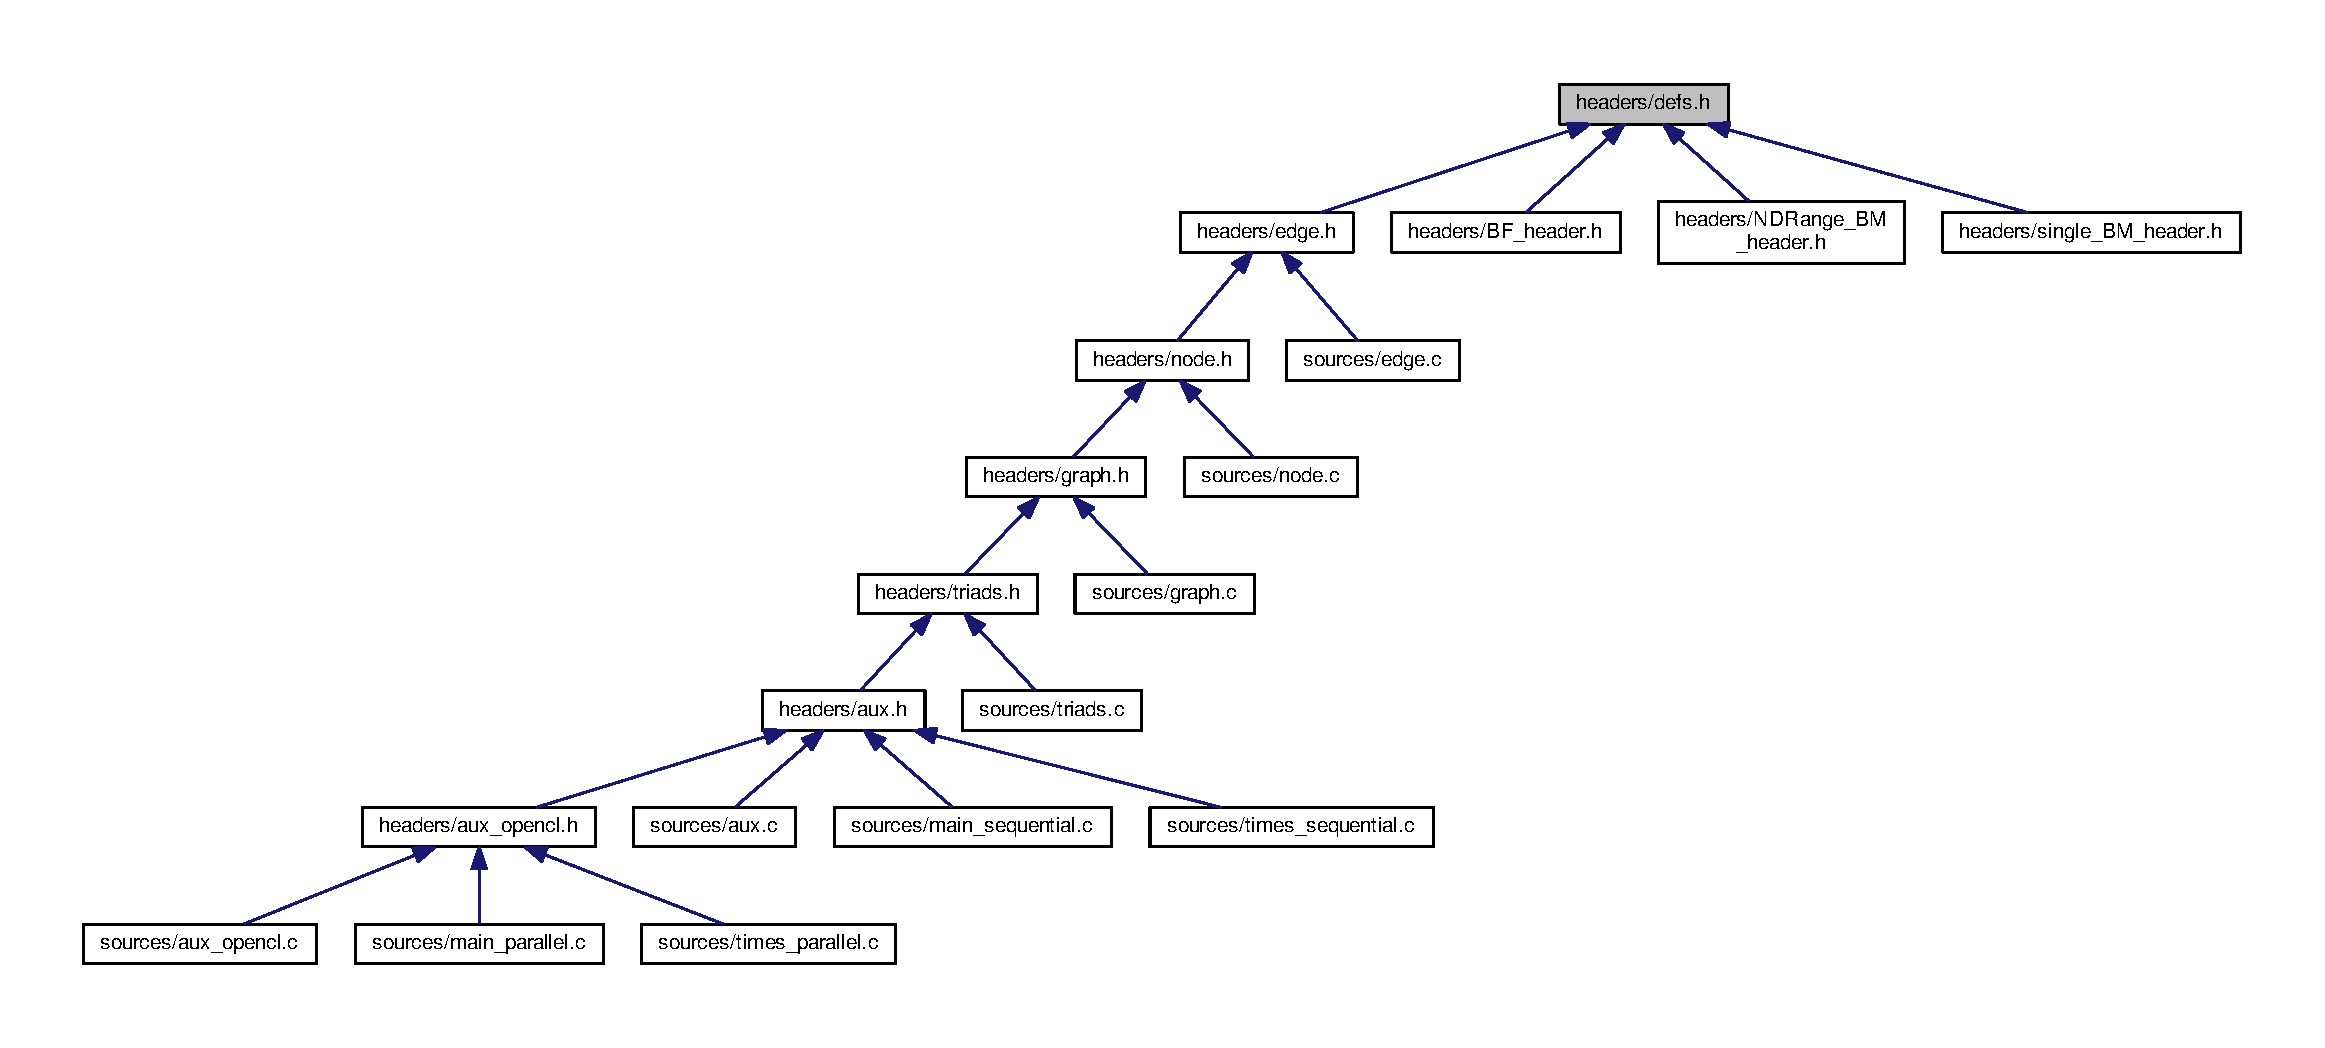
\includegraphics[width=350pt]{defs_8h__dep__incl}
\end{center}
\end{figure}
\subsection*{Data Structures}
\begin{DoxyCompactItemize}
\item 
struct \hyperlink{structNODE__DEVICE}{N\+O\+D\+E\+\_\+\+D\+E\+V\+I\+CE}
\begin{DoxyCompactList}\small\item\em This structure stores the information of a node within the graph. This structure is used in the kernel code and executed on the F\+P\+GA. \end{DoxyCompactList}\item 
struct \hyperlink{structTASK}{T\+A\+SK}
\begin{DoxyCompactList}\small\item\em This structure contains the information of a pair of nodes (u,v). Each pair of nodes is processed by a different kernel instance on a S\+I\+MD manner This structure is used in the kernel code and executed on the F\+P\+GA. \end{DoxyCompactList}\item 
struct \hyperlink{structCENSUS}{C\+E\+N\+S\+US}
\begin{DoxyCompactList}\small\item\em This structure contains a 16-\/position census array Each instance of an N\+D\+Range kernel has a different census array in which to write local results. This structure is used in the kernel code and executed on the F\+P\+GA. \end{DoxyCompactList}\end{DoxyCompactItemize}
\subsection*{Typedefs}
\begin{DoxyCompactItemize}
\item 
typedef unsigned int \hyperlink{defs_8h_aadb1697eee3bb21dd6aa3af50b858d29}{E\+D\+G\+E\+\_\+\+D\+E\+V\+I\+CE}
\end{DoxyCompactItemize}


\subsection{Detailed Description}
This file contains the definitions of the structures that are used for the kernel code. 

\begin{DoxyAuthor}{Author}
\+: Carlos Alfaro
\end{DoxyAuthor}
\begin{DoxyDate}{Date}
\+: 13-\/12-\/2017 
\end{DoxyDate}


\subsection{Typedef Documentation}
\mbox{\Hypertarget{defs_8h_aadb1697eee3bb21dd6aa3af50b858d29}\label{defs_8h_aadb1697eee3bb21dd6aa3af50b858d29}} 
\index{defs.\+h@{defs.\+h}!E\+D\+G\+E\+\_\+\+D\+E\+V\+I\+CE@{E\+D\+G\+E\+\_\+\+D\+E\+V\+I\+CE}}
\index{E\+D\+G\+E\+\_\+\+D\+E\+V\+I\+CE@{E\+D\+G\+E\+\_\+\+D\+E\+V\+I\+CE}!defs.\+h@{defs.\+h}}
\subsubsection{\texorpdfstring{E\+D\+G\+E\+\_\+\+D\+E\+V\+I\+CE}{EDGE\_DEVICE}}
{\footnotesize\ttfamily typedef unsigned int \hyperlink{structEDGE__DEVICE}{E\+D\+G\+E\+\_\+\+D\+E\+V\+I\+CE}}

Stores the neighbor id and the direction of the edge 
\hypertarget{edge_8h}{}\section{headers/edge.h File Reference}
\label{edge_8h}\index{headers/edge.\+h@{headers/edge.\+h}}


This file contains the definitions of the functions needed to create and manage an edge of a graph.  within project, we consider only directed graphs; edges must have a direction. ~\newline
In our implementation, edge information is saved twice, since each of the nodes keeps its adjacency list (see \hyperlink{node_8h}{node.\+h}).~\newline
 Each edge structure is therefore part of the node it belongs to, and contains the id of the other neigbhbor, and the direction.~\newline
 The direction is coded using the 2 less significant bits of the uint32\+\_\+t used for storing the edge.~\newline
 \textquotesingle{}01\textquotesingle{} means that the edge goes out from the node it belongs, \textquotesingle{}10\textquotesingle{} means edge goes in, and \textquotesingle{}11\textquotesingle{} conveys bidirectionality.  


{\ttfamily \#include \char`\"{}defs.\+h\char`\"{}}\newline
{\ttfamily \#include $<$inttypes.\+h$>$}\newline
{\ttfamily \#include $<$stdio.\+h$>$}\newline
{\ttfamily \#include $<$stdlib.\+h$>$}\newline
Include dependency graph for edge.\+h\+:\nopagebreak
\begin{figure}[H]
\begin{center}
\leavevmode
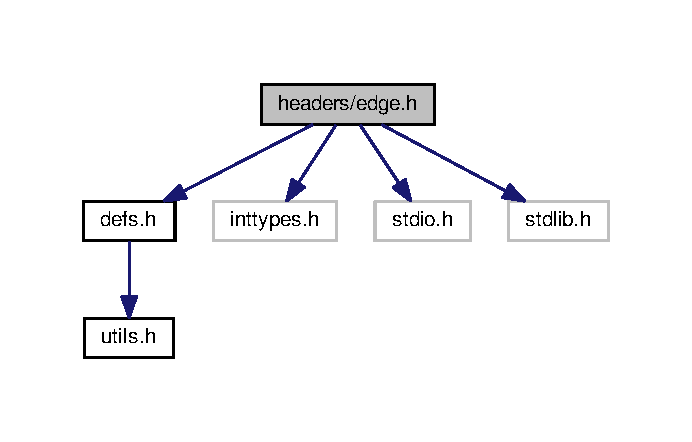
\includegraphics[width=332pt]{edge_8h__incl}
\end{center}
\end{figure}
This graph shows which files directly or indirectly include this file\+:
\nopagebreak
\begin{figure}[H]
\begin{center}
\leavevmode
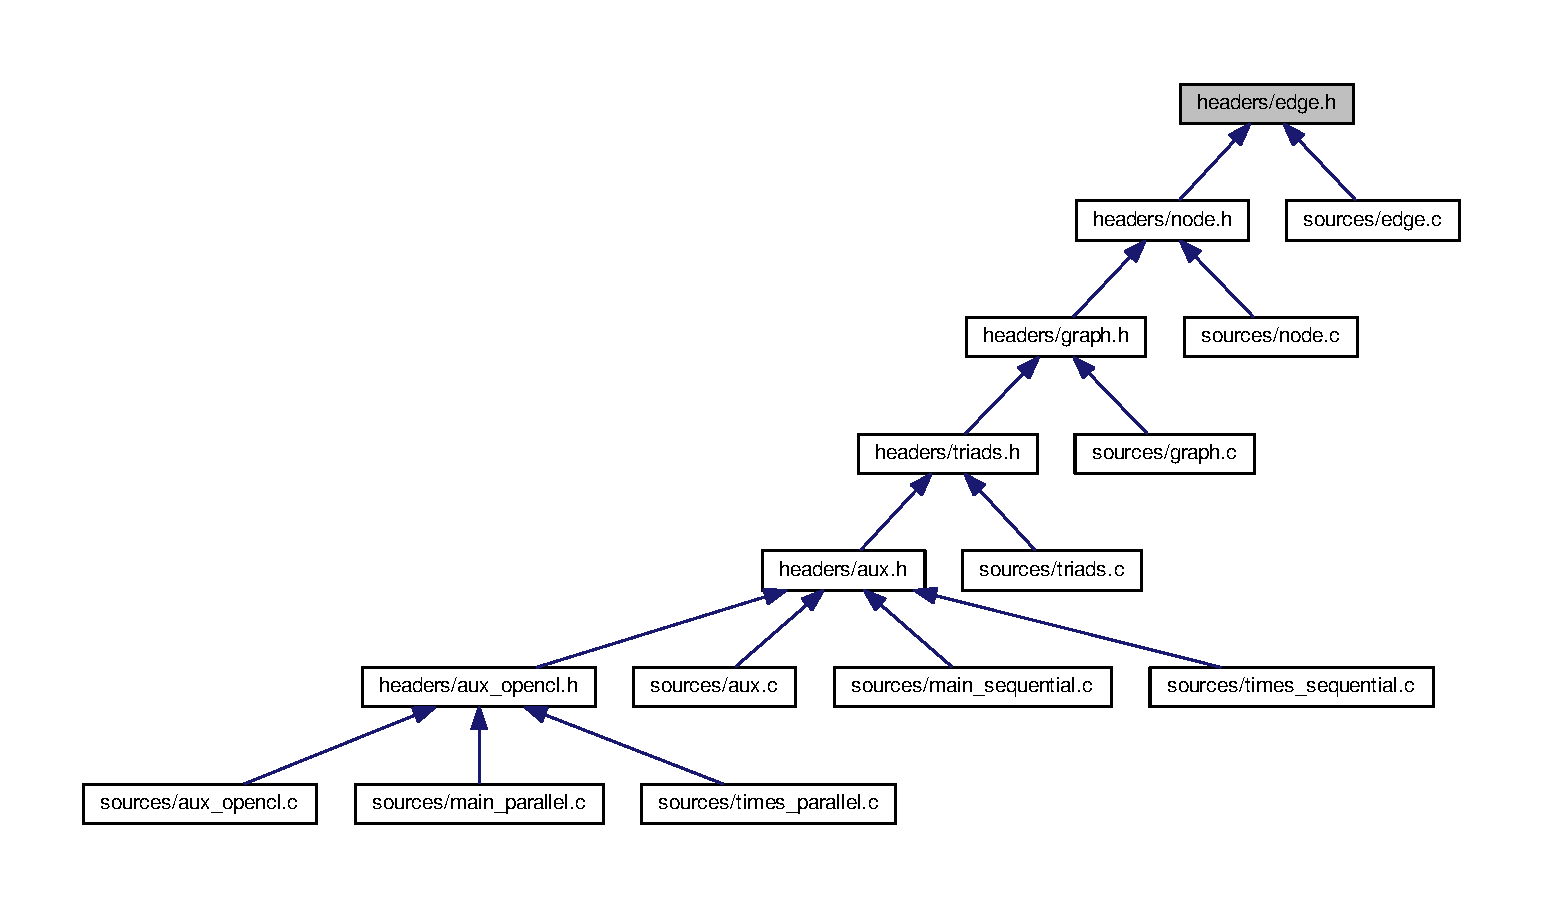
\includegraphics[width=350pt]{edge_8h__dep__incl}
\end{center}
\end{figure}
\subsection*{Typedefs}
\begin{DoxyCompactItemize}
\item 
typedef uint32\+\_\+t \hyperlink{edge_8h_ab4a642fc78a44ca8df119570b3288e13}{E\+D\+GE}
\end{DoxyCompactItemize}
\subsection*{Functions}
\begin{DoxyCompactItemize}
\item 
\hyperlink{edge_8h_ab4a642fc78a44ca8df119570b3288e13}{E\+D\+GE} \hyperlink{edge_8h_a15ac9743daa3a7d6ade50b68d6de86eb}{create\+\_\+edge} (uint32\+\_\+t edge\+\_\+id, \hyperlink{utils_8h_aa268a41a13430b18e933ed40207178d0}{D\+I\+R\+E\+C\+T\+I\+ON} dir)
\begin{DoxyCompactList}\small\item\em Function that creates an E\+D\+GE from a node id and a direction. \end{DoxyCompactList}\item 
uint32\+\_\+t \hyperlink{edge_8h_ad9aa111cad82e20619c31f7fc8cc8c96}{get\+\_\+neighbor\+\_\+id} (\hyperlink{edge_8h_ab4a642fc78a44ca8df119570b3288e13}{E\+D\+GE} e)
\begin{DoxyCompactList}\small\item\em Function that returns the neighbor id of an edge. \end{DoxyCompactList}\item 
\hyperlink{utils_8h_aa268a41a13430b18e933ed40207178d0}{D\+I\+R\+E\+C\+T\+I\+ON} \hyperlink{edge_8h_a1038dbe86b3582aa654a201c791b9293}{get\+\_\+direction} (\hyperlink{edge_8h_ab4a642fc78a44ca8df119570b3288e13}{E\+D\+GE} e)
\begin{DoxyCompactList}\small\item\em Function that returns the direction of an edge. \end{DoxyCompactList}\item 
\hyperlink{utils_8h_a32c27cc471df37f4fc818d65de0a56c4}{S\+T\+A\+T\+US} \hyperlink{edge_8h_afb1416581aec9a56ad9354e3826a9fd7}{set\+\_\+direction} (\hyperlink{edge_8h_ab4a642fc78a44ca8df119570b3288e13}{E\+D\+GE} $\ast$e, \hyperlink{utils_8h_aa268a41a13430b18e933ed40207178d0}{D\+I\+R\+E\+C\+T\+I\+ON} dir)
\begin{DoxyCompactList}\small\item\em Function that sets the direction of an edge. \end{DoxyCompactList}\item 
int \hyperlink{edge_8h_afe003267551a5687d635d20f78f00c84}{comp\+\_\+edges} (const void $\ast$e1, const void $\ast$e2)
\begin{DoxyCompactList}\small\item\em Function that compares to edges based on the neighbor ids. \end{DoxyCompactList}\item 
void \hyperlink{edge_8h_a4be4f5fd773a94c7a53773a54906ad02}{insert\+\_\+edge} (void $\ast$adj\+\_\+list, void $\ast$e, int pos)
\begin{DoxyCompactList}\small\item\em Function that inserts an edge in an adjacency lists. \end{DoxyCompactList}\item 
void \hyperlink{edge_8h_a41ae2473935226d4734adcb6e2c8ccaa}{print\+\_\+edge} (uint32\+\_\+t in, \hyperlink{edge_8h_ab4a642fc78a44ca8df119570b3288e13}{E\+D\+GE} e)
\begin{DoxyCompactList}\small\item\em Function prints an edge. \end{DoxyCompactList}\end{DoxyCompactItemize}


\subsection{Detailed Description}
This file contains the definitions of the functions needed to create and manage an edge of a graph.  within project, we consider only directed graphs; edges must have a direction. ~\newline
In our implementation, edge information is saved twice, since each of the nodes keeps its adjacency list (see \hyperlink{node_8h}{node.\+h}).~\newline
 Each edge structure is therefore part of the node it belongs to, and contains the id of the other neigbhbor, and the direction.~\newline
 The direction is coded using the 2 less significant bits of the uint32\+\_\+t used for storing the edge.~\newline
 \textquotesingle{}01\textquotesingle{} means that the edge goes out from the node it belongs, \textquotesingle{}10\textquotesingle{} means edge goes in, and \textquotesingle{}11\textquotesingle{} conveys bidirectionality. 

\begin{DoxyAuthor}{Author}
\+: Carlos Alfaro
\end{DoxyAuthor}
\begin{DoxyDate}{Date}
\+: 23-\/10-\/2017 
\end{DoxyDate}


\subsection{Typedef Documentation}
\mbox{\Hypertarget{edge_8h_ab4a642fc78a44ca8df119570b3288e13}\label{edge_8h_ab4a642fc78a44ca8df119570b3288e13}} 
\index{edge.\+h@{edge.\+h}!E\+D\+GE@{E\+D\+GE}}
\index{E\+D\+GE@{E\+D\+GE}!edge.\+h@{edge.\+h}}
\subsubsection{\texorpdfstring{E\+D\+GE}{EDGE}}
{\footnotesize\ttfamily typedef uint32\+\_\+t \hyperlink{edge_8h_ab4a642fc78a44ca8df119570b3288e13}{E\+D\+GE}}

An edge is coded as an unsigned integer of 32 bits. 

\subsection{Function Documentation}
\mbox{\Hypertarget{edge_8h_afe003267551a5687d635d20f78f00c84}\label{edge_8h_afe003267551a5687d635d20f78f00c84}} 
\index{edge.\+h@{edge.\+h}!comp\+\_\+edges@{comp\+\_\+edges}}
\index{comp\+\_\+edges@{comp\+\_\+edges}!edge.\+h@{edge.\+h}}
\subsubsection{\texorpdfstring{comp\+\_\+edges()}{comp\_edges()}}
{\footnotesize\ttfamily int comp\+\_\+edges (\begin{DoxyParamCaption}\item[{const void $\ast$}]{e1,  }\item[{const void $\ast$}]{e2 }\end{DoxyParamCaption})}



Function that compares to edges based on the neighbor ids. 


\begin{DoxyParams}{Parameters}
{\em const} & void$\ast$ e1\+: First edge \\
\hline
{\em const} & void$\ast$ e2\+: Second edge\\
\hline
\end{DoxyParams}
\begin{DoxyReturn}{Returns}
int\+: a value less than, equal to or greater than 0 ~\newline
depending on whether e1 is smaller than, equal or greater ~\newline
than e2, respectively 
\end{DoxyReturn}
\mbox{\Hypertarget{edge_8h_a15ac9743daa3a7d6ade50b68d6de86eb}\label{edge_8h_a15ac9743daa3a7d6ade50b68d6de86eb}} 
\index{edge.\+h@{edge.\+h}!create\+\_\+edge@{create\+\_\+edge}}
\index{create\+\_\+edge@{create\+\_\+edge}!edge.\+h@{edge.\+h}}
\subsubsection{\texorpdfstring{create\+\_\+edge()}{create\_edge()}}
{\footnotesize\ttfamily \hyperlink{edge_8h_ab4a642fc78a44ca8df119570b3288e13}{E\+D\+GE} create\+\_\+edge (\begin{DoxyParamCaption}\item[{uint32\+\_\+t}]{edge\+\_\+id,  }\item[{\hyperlink{utils_8h_aa268a41a13430b18e933ed40207178d0}{D\+I\+R\+E\+C\+T\+I\+ON}}]{dir }\end{DoxyParamCaption})}



Function that creates an E\+D\+GE from a node id and a direction. 


\begin{DoxyParams}{Parameters}
{\em uint32\+\_\+t} & edge\+\_\+id\+: id of the neighbor node \\
\hline
{\em D\+I\+R\+E\+C\+T\+I\+ON} & dir\+: direction of the edge\\
\hline
\end{DoxyParams}
\begin{DoxyReturn}{Returns}
E\+D\+GE\+: the new created edge 
\end{DoxyReturn}
\mbox{\Hypertarget{edge_8h_a1038dbe86b3582aa654a201c791b9293}\label{edge_8h_a1038dbe86b3582aa654a201c791b9293}} 
\index{edge.\+h@{edge.\+h}!get\+\_\+direction@{get\+\_\+direction}}
\index{get\+\_\+direction@{get\+\_\+direction}!edge.\+h@{edge.\+h}}
\subsubsection{\texorpdfstring{get\+\_\+direction()}{get\_direction()}}
{\footnotesize\ttfamily \hyperlink{utils_8h_aa268a41a13430b18e933ed40207178d0}{D\+I\+R\+E\+C\+T\+I\+ON} get\+\_\+direction (\begin{DoxyParamCaption}\item[{\hyperlink{edge_8h_ab4a642fc78a44ca8df119570b3288e13}{E\+D\+GE}}]{e }\end{DoxyParamCaption})}



Function that returns the direction of an edge. 


\begin{DoxyParams}{Parameters}
{\em E\+D\+GE} & e\+: The edge\\
\hline
\end{DoxyParams}
\begin{DoxyReturn}{Returns}
D\+I\+R\+E\+C\+T\+I\+ON\+: The direction of the edge 
\end{DoxyReturn}
\mbox{\Hypertarget{edge_8h_ad9aa111cad82e20619c31f7fc8cc8c96}\label{edge_8h_ad9aa111cad82e20619c31f7fc8cc8c96}} 
\index{edge.\+h@{edge.\+h}!get\+\_\+neighbor\+\_\+id@{get\+\_\+neighbor\+\_\+id}}
\index{get\+\_\+neighbor\+\_\+id@{get\+\_\+neighbor\+\_\+id}!edge.\+h@{edge.\+h}}
\subsubsection{\texorpdfstring{get\+\_\+neighbor\+\_\+id()}{get\_neighbor\_id()}}
{\footnotesize\ttfamily uint32\+\_\+t get\+\_\+neighbor\+\_\+id (\begin{DoxyParamCaption}\item[{\hyperlink{edge_8h_ab4a642fc78a44ca8df119570b3288e13}{E\+D\+GE}}]{e }\end{DoxyParamCaption})}



Function that returns the neighbor id of an edge. 


\begin{DoxyParams}{Parameters}
{\em E\+D\+GE} & e\+: The edge\\
\hline
\end{DoxyParams}
\begin{DoxyReturn}{Returns}
uint32\+\_\+t\+: The neighbor id 
\end{DoxyReturn}
\mbox{\Hypertarget{edge_8h_a4be4f5fd773a94c7a53773a54906ad02}\label{edge_8h_a4be4f5fd773a94c7a53773a54906ad02}} 
\index{edge.\+h@{edge.\+h}!insert\+\_\+edge@{insert\+\_\+edge}}
\index{insert\+\_\+edge@{insert\+\_\+edge}!edge.\+h@{edge.\+h}}
\subsubsection{\texorpdfstring{insert\+\_\+edge()}{insert\_edge()}}
{\footnotesize\ttfamily void insert\+\_\+edge (\begin{DoxyParamCaption}\item[{void $\ast$}]{adj\+\_\+list,  }\item[{void $\ast$}]{e,  }\item[{int}]{pos }\end{DoxyParamCaption})}



Function that inserts an edge in an adjacency lists. 


\begin{DoxyParams}{Parameters}
{\em void$\ast$} & adj\+\_\+list\+: array where to insert the edge \\
\hline
{\em void$\ast$} & edge\+: Edge to insert \\
\hline
{\em int} & pos\+: The position where to insert\\
\hline
\end{DoxyParams}
\begin{DoxyReturn}{Returns}
None 
\end{DoxyReturn}
\mbox{\Hypertarget{edge_8h_a41ae2473935226d4734adcb6e2c8ccaa}\label{edge_8h_a41ae2473935226d4734adcb6e2c8ccaa}} 
\index{edge.\+h@{edge.\+h}!print\+\_\+edge@{print\+\_\+edge}}
\index{print\+\_\+edge@{print\+\_\+edge}!edge.\+h@{edge.\+h}}
\subsubsection{\texorpdfstring{print\+\_\+edge()}{print\_edge()}}
{\footnotesize\ttfamily void print\+\_\+edge (\begin{DoxyParamCaption}\item[{uint32\+\_\+t}]{in,  }\item[{\hyperlink{edge_8h_ab4a642fc78a44ca8df119570b3288e13}{E\+D\+GE}}]{e }\end{DoxyParamCaption})}



Function prints an edge. 


\begin{DoxyParams}{Parameters}
{\em uint32\+\_\+t} & in\+: the node id from where the node goes out \\
\hline
{\em E\+D\+GE} & e\+: The edge to print\\
\hline
\end{DoxyParams}
\begin{DoxyReturn}{Returns}
None 
\end{DoxyReturn}
\mbox{\Hypertarget{edge_8h_afb1416581aec9a56ad9354e3826a9fd7}\label{edge_8h_afb1416581aec9a56ad9354e3826a9fd7}} 
\index{edge.\+h@{edge.\+h}!set\+\_\+direction@{set\+\_\+direction}}
\index{set\+\_\+direction@{set\+\_\+direction}!edge.\+h@{edge.\+h}}
\subsubsection{\texorpdfstring{set\+\_\+direction()}{set\_direction()}}
{\footnotesize\ttfamily \hyperlink{utils_8h_a32c27cc471df37f4fc818d65de0a56c4}{S\+T\+A\+T\+US} set\+\_\+direction (\begin{DoxyParamCaption}\item[{\hyperlink{edge_8h_ab4a642fc78a44ca8df119570b3288e13}{E\+D\+GE} $\ast$}]{e,  }\item[{\hyperlink{utils_8h_aa268a41a13430b18e933ed40207178d0}{D\+I\+R\+E\+C\+T\+I\+ON}}]{dir }\end{DoxyParamCaption})}



Function that sets the direction of an edge. 


\begin{DoxyParams}{Parameters}
{\em E\+D\+GE} & e\+: The edge we want to modify \\
\hline
{\em D\+I\+R\+E\+C\+T\+I\+ON} & dir\+: The direction to set\\
\hline
\end{DoxyParams}
\begin{DoxyReturn}{Returns}
S\+T\+A\+T\+US\+: OK if the operation was successful~\newline
 E\+RR otherwise 
\end{DoxyReturn}

\hypertarget{graph_8h}{}\section{headers/graph.h File Reference}
\label{graph_8h}\index{headers/graph.\+h@{headers/graph.\+h}}


This file contains the definitions of the functions needed to create and manage a graph. ~\newline
In our implementation, the graph is read from a file which, in each of its lines, contains an edge of the graph in this format\+:~\newline
 src\+\_\+node\+\_\+id tgt\+\_\+node\+\_\+id ~\newline
In the structure, nodes can be ordered by ascending order of their ids.  


{\ttfamily \#include \char`\"{}node.\+h\char`\"{}}\newline
Include dependency graph for graph.\+h\+:\nopagebreak
\begin{figure}[H]
\begin{center}
\leavevmode
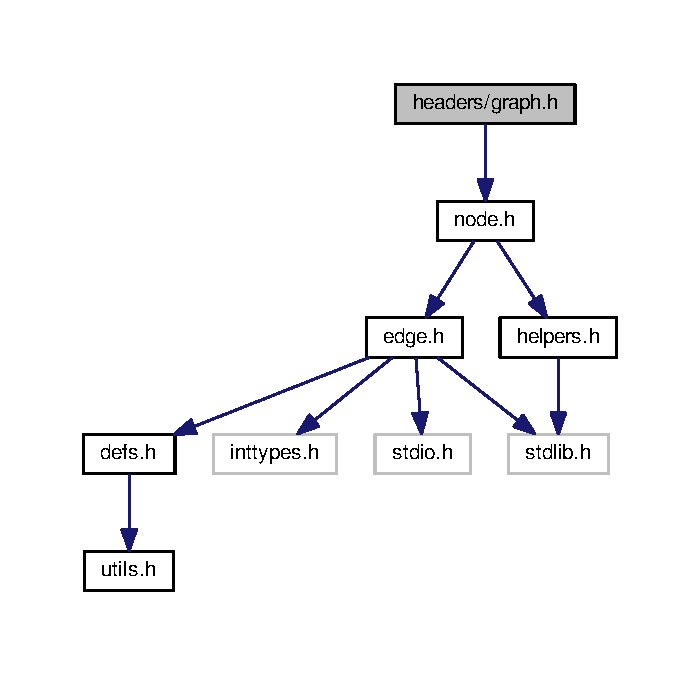
\includegraphics[width=336pt]{graph_8h__incl}
\end{center}
\end{figure}
This graph shows which files directly or indirectly include this file\+:\nopagebreak
\begin{figure}[H]
\begin{center}
\leavevmode
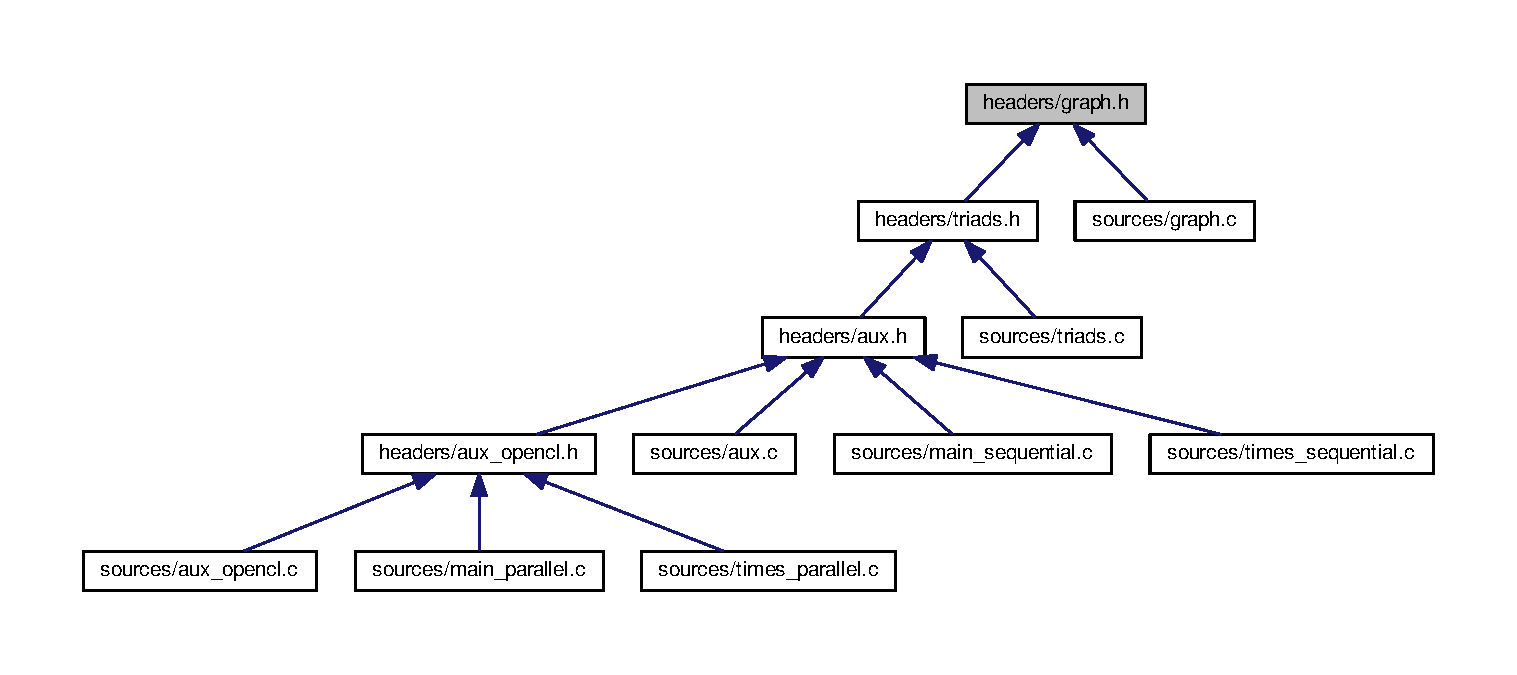
\includegraphics[width=192pt]{graph_8h__dep__incl}
\end{center}
\end{figure}
\subsection*{Data Structures}
\begin{DoxyCompactItemize}
\item 
struct \hyperlink{structGRAPH}{G\+R\+A\+PH}
\begin{DoxyCompactList}\small\item\em This structure stores the necessary graph information. \end{DoxyCompactList}\end{DoxyCompactItemize}
\subsection*{Functions}
\begin{DoxyCompactItemize}
\item 
void \hyperlink{graph_8h_aa4ecaf8c04f3465eb1fd3c0a74927669}{set\+\_\+ordered} (\hyperlink{utils_8h_a3e5b8192e7d9ffaf3542f1210aec18dd}{B\+O\+OL} value)
\begin{DoxyCompactList}\small\item\em Function that sets the global variable ordered to a certain value passed as a parameter. \end{DoxyCompactList}\item 
\hyperlink{structGRAPH}{G\+R\+A\+PH} $\ast$ \hyperlink{graph_8h_a1e691638038900c9478325f5dbd66e0e}{read\+\_\+graph\+\_\+from\+\_\+file} (char $\ast$filename)
\begin{DoxyCompactList}\small\item\em Function that reads the file containing the graph information,~\newline
 and creates the \hyperlink{structGRAPH}{G\+R\+A\+PH} structure, returning a pointer to it. \end{DoxyCompactList}\item 
\hyperlink{utils_8h_a32c27cc471df37f4fc818d65de0a56c4}{S\+T\+A\+T\+US} \hyperlink{graph_8h_a00c645263fd09257dcc7d7f790a8a139}{insert\+\_\+node} (\hyperlink{structGRAPH}{G\+R\+A\+PH} $\ast$g, uint32\+\_\+t node\+\_\+id)
\begin{DoxyCompactList}\small\item\em Function that inserts a node in the graph. \end{DoxyCompactList}\item 
\hyperlink{utils_8h_a32c27cc471df37f4fc818d65de0a56c4}{S\+T\+A\+T\+US} \hyperlink{graph_8h_ac54e6c3dd8086e0d0054866fcb48c8fa}{add\+\_\+edge} (\hyperlink{structGRAPH}{G\+R\+A\+PH} $\ast$g, uint32\+\_\+t node\+\_\+id1, uint32\+\_\+t node\+\_\+id2, \hyperlink{utils_8h_aa268a41a13430b18e933ed40207178d0}{D\+I\+R\+E\+C\+T\+I\+ON} dir)
\begin{DoxyCompactList}\small\item\em Function that adds an edge to a certain node. To add an edge e,~\newline
we need to have the ids of the two nodes that the e connects; ant its ~\newline
direction. The function basically adds the edge to the adjacency list of~\newline
the node with id node\+\_\+id1, setting the neighbor id of the edge to node\+\_\+id2. \end{DoxyCompactList}\item 
\hyperlink{utils_8h_a3e5b8192e7d9ffaf3542f1210aec18dd}{B\+O\+OL} \hyperlink{graph_8h_a327ad76c2c67dc829facce47bb987de3}{node\+\_\+exists} (\hyperlink{structGRAPH}{G\+R\+A\+PH} $\ast$g, uint32\+\_\+t node\+\_\+id)
\begin{DoxyCompactList}\small\item\em Function that checks whether a node is present in a graph. \end{DoxyCompactList}\item 
int \hyperlink{graph_8h_a958ec048e564a498f7e2fb6eea436d35}{get\+\_\+node\+\_\+pos} (\hyperlink{structGRAPH}{G\+R\+A\+PH} $\ast$g, uint32\+\_\+t node\+\_\+id)
\begin{DoxyCompactList}\small\item\em Function that obtains the position of the node with id node\+\_\+id within the ~\newline
array of nodes of graph g. \end{DoxyCompactList}\item 
uint32\+\_\+t \hyperlink{graph_8h_ab655a5453feb3f96ed28d14dd192287b}{get\+\_\+num\+\_\+nodes} (const \hyperlink{structGRAPH}{G\+R\+A\+PH} $\ast$g)
\begin{DoxyCompactList}\small\item\em Function that obtains the number of nodes of a graph g. \end{DoxyCompactList}\item 
uint32\+\_\+t \hyperlink{graph_8h_ac472a365756f3728c133b4cba52127d3}{get\+\_\+num\+\_\+pairs} (const \hyperlink{structGRAPH}{G\+R\+A\+PH} $\ast$g)
\begin{DoxyCompactList}\small\item\em Function that obtains the number of pairs (u,v) of nodes in graph g. \end{DoxyCompactList}\item 
uint64\+\_\+t \hyperlink{graph_8h_a17c6c18decd7024d45439e01aa4f359e}{get\+\_\+num\+\_\+triples} (const \hyperlink{structGRAPH}{G\+R\+A\+PH} $\ast$g)
\begin{DoxyCompactList}\small\item\em Function that obtains the number of triples (u,v,w) of nodes in graph g. \end{DoxyCompactList}\item 
uint32\+\_\+t \hyperlink{graph_8h_a69902bced6cd88bc38dd7c863b367dfc}{get\+\_\+num\+\_\+edges} (const \hyperlink{structGRAPH}{G\+R\+A\+PH} $\ast$g)
\begin{DoxyCompactList}\small\item\em Function that obtains the number of edges of ha graph g. \end{DoxyCompactList}\item 
\hyperlink{structNODE}{N\+O\+DE} $\ast$ \hyperlink{graph_8h_a15242f86399df5a7fcac2127c5606461}{get\+\_\+node\+\_\+by\+\_\+pos} (const \hyperlink{structGRAPH}{G\+R\+A\+PH} $\ast$g, int pos)
\begin{DoxyCompactList}\small\item\em Function that obtains the node of graph g present in position pos. \end{DoxyCompactList}\item 
\hyperlink{structNODE}{N\+O\+DE} $\ast$ \hyperlink{graph_8h_a479b13695ab11c89b03a81cf70ca889b}{get\+\_\+node\+\_\+by\+\_\+id} (\hyperlink{structGRAPH}{G\+R\+A\+PH} $\ast$g, uint32\+\_\+t node\+\_\+id)
\begin{DoxyCompactList}\small\item\em Function that obtains the node of graph g that has id node\+\_\+id. \end{DoxyCompactList}\item 
void \hyperlink{graph_8h_a4d6f9793800397e068b0031d7ba42bba}{print\+\_\+graph} (\hyperlink{structGRAPH}{G\+R\+A\+PH} $\ast$g)
\begin{DoxyCompactList}\small\item\em Function that prints the information of graph. \end{DoxyCompactList}\item 
void \hyperlink{graph_8h_a496da63fdfc498a7e901f2a65a39ffe8}{destroy\+\_\+graph} (\hyperlink{structGRAPH}{G\+R\+A\+PH} $\ast$g)
\begin{DoxyCompactList}\small\item\em Function that destroys a graph, freeing the memory of its structures. \end{DoxyCompactList}\item 
\hyperlink{utils_8h_a32c27cc471df37f4fc818d65de0a56c4}{S\+T\+A\+T\+US} \hyperlink{graph_8h_a5aab9084b4ffec389343766cf27bf752}{convert\+\_\+graph} (\hyperlink{structGRAPH}{G\+R\+A\+PH} $\ast$g, \hyperlink{structNODE__DEVICE}{N\+O\+D\+E\+\_\+\+D\+E\+V\+I\+CE} $\ast$$\ast$nodes, \hyperlink{structEDGE__DEVICE}{E\+D\+G\+E\+\_\+\+D\+E\+V\+I\+CE} $\ast$$\ast$edges, uint32\+\_\+t $\ast$num\+\_\+nodes, uint32\+\_\+t $\ast$num\+\_\+edges)
\begin{DoxyCompactList}\small\item\em Function that, given a graph, constructs the array of nodes and edges,~\newline
 which is a suitable saving format for processing the graph in the device. \end{DoxyCompactList}\item 
\hyperlink{structTASK}{T\+A\+SK} $\ast$ \hyperlink{graph_8h_a918eb6777060cb3eecf14703db2b1b76}{create\+\_\+tasks\+\_\+array} (\hyperlink{structGRAPH}{G\+R\+A\+PH} $\ast$g, \hyperlink{structNODE__DEVICE}{N\+O\+D\+E\+\_\+\+D\+E\+V\+I\+CE} $\ast$nodes, uint32\+\_\+t $\ast$num\+\_\+tasks)
\begin{DoxyCompactList}\small\item\em Function that creates an array of tasks. \end{DoxyCompactList}\end{DoxyCompactItemize}


\subsection{Detailed Description}
This file contains the definitions of the functions needed to create and manage a graph. ~\newline
In our implementation, the graph is read from a file which, in each of its lines, contains an edge of the graph in this format\+:~\newline
 src\+\_\+node\+\_\+id tgt\+\_\+node\+\_\+id ~\newline
In the structure, nodes can be ordered by ascending order of their ids. 

\begin{DoxyAuthor}{Author}
\+: Carlos Alfaro
\end{DoxyAuthor}
\begin{DoxyDate}{Date}
\+: 23-\/10-\/2017 
\end{DoxyDate}


\subsection{Function Documentation}
\mbox{\Hypertarget{graph_8h_ac54e6c3dd8086e0d0054866fcb48c8fa}\label{graph_8h_ac54e6c3dd8086e0d0054866fcb48c8fa}} 
\index{graph.\+h@{graph.\+h}!add\+\_\+edge@{add\+\_\+edge}}
\index{add\+\_\+edge@{add\+\_\+edge}!graph.\+h@{graph.\+h}}
\subsubsection{\texorpdfstring{add\+\_\+edge()}{add\_edge()}}
{\footnotesize\ttfamily \hyperlink{utils_8h_a32c27cc471df37f4fc818d65de0a56c4}{S\+T\+A\+T\+US} add\+\_\+edge (\begin{DoxyParamCaption}\item[{\hyperlink{structGRAPH}{G\+R\+A\+PH} $\ast$}]{g,  }\item[{uint32\+\_\+t}]{node\+\_\+id1,  }\item[{uint32\+\_\+t}]{node\+\_\+id2,  }\item[{\hyperlink{utils_8h_aa268a41a13430b18e933ed40207178d0}{D\+I\+R\+E\+C\+T\+I\+ON}}]{dir }\end{DoxyParamCaption})}



Function that adds an edge to a certain node. To add an edge e,~\newline
we need to have the ids of the two nodes that the e connects; ant its ~\newline
direction. The function basically adds the edge to the adjacency list of~\newline
the node with id node\+\_\+id1, setting the neighbor id of the edge to node\+\_\+id2. 


\begin{DoxyParams}{Parameters}
{\em G\+R\+A\+P\+H$\ast$} & g\+: The graph in which we want to add the edge \\
\hline
{\em uint32\+\_\+t} & node\+\_\+id1\+: The id of one of the nodes of the edge \\
\hline
{\em uint32\+\_\+t} & node\+\_\+id2\+: The id of the other id \\
\hline
{\em D\+I\+R\+E\+C\+T\+I\+ON} & dir\+: The direction of the edge\+:  if it goes from id1 to id2.~\newline
 O\+U\+T\+\_\+\+IN if it goes from id2 to id1.\\
\hline
\end{DoxyParams}
\begin{DoxyReturn}{Returns}
S\+T\+A\+T\+US\+: OK if the insertion was successful. E\+RR otherwise 
\end{DoxyReturn}
\mbox{\Hypertarget{graph_8h_a5aab9084b4ffec389343766cf27bf752}\label{graph_8h_a5aab9084b4ffec389343766cf27bf752}} 
\index{graph.\+h@{graph.\+h}!convert\+\_\+graph@{convert\+\_\+graph}}
\index{convert\+\_\+graph@{convert\+\_\+graph}!graph.\+h@{graph.\+h}}
\subsubsection{\texorpdfstring{convert\+\_\+graph()}{convert\_graph()}}
{\footnotesize\ttfamily \hyperlink{utils_8h_a32c27cc471df37f4fc818d65de0a56c4}{S\+T\+A\+T\+US} convert\+\_\+graph (\begin{DoxyParamCaption}\item[{\hyperlink{structGRAPH}{G\+R\+A\+PH} $\ast$}]{g,  }\item[{\hyperlink{structNODE__DEVICE}{N\+O\+D\+E\+\_\+\+D\+E\+V\+I\+CE} $\ast$$\ast$}]{nodes,  }\item[{\hyperlink{structEDGE__DEVICE}{E\+D\+G\+E\+\_\+\+D\+E\+V\+I\+CE} $\ast$$\ast$}]{edges,  }\item[{uint32\+\_\+t $\ast$}]{num\+\_\+nodes,  }\item[{uint32\+\_\+t $\ast$}]{num\+\_\+edges }\end{DoxyParamCaption})}



Function that, given a graph, constructs the array of nodes and edges,~\newline
 which is a suitable saving format for processing the graph in the device. 


\begin{DoxyParams}{Parameters}
{\em G\+R\+A\+P\+H$\ast$} & g\+: the graph to convert \\
\hline
{\em N\+O\+D\+E\+\_\+\+D\+E\+V\+I\+C\+E$\ast$$\ast$} & nodes\+: A pointer to the array of nodes (to be filled) \\
\hline
{\em E\+D\+G\+E\+\_\+\+D\+E\+V\+I\+C\+E$\ast$$\ast$} & edges\+: A pointer to the array of edges (to be filled) \\
\hline
{\em uint32\+\_\+t$\ast$} & num\+\_\+nodes\+: The number of nodes, (to be filled) \\
\hline
{\em uint32\+\_\+t$\ast$} & num\+\_\+edges\+: The number of edges (to be filled)\\
\hline
\end{DoxyParams}
\begin{DoxyReturn}{Returns}
S\+T\+A\+T\+US\+: OK if the arrays were constructed correctly, E\+RR otherwise 
\end{DoxyReturn}
\mbox{\Hypertarget{graph_8h_a918eb6777060cb3eecf14703db2b1b76}\label{graph_8h_a918eb6777060cb3eecf14703db2b1b76}} 
\index{graph.\+h@{graph.\+h}!create\+\_\+tasks\+\_\+array@{create\+\_\+tasks\+\_\+array}}
\index{create\+\_\+tasks\+\_\+array@{create\+\_\+tasks\+\_\+array}!graph.\+h@{graph.\+h}}
\subsubsection{\texorpdfstring{create\+\_\+tasks\+\_\+array()}{create\_tasks\_array()}}
{\footnotesize\ttfamily \hyperlink{structTASK}{T\+A\+SK}$\ast$ create\+\_\+tasks\+\_\+array (\begin{DoxyParamCaption}\item[{\hyperlink{structGRAPH}{G\+R\+A\+PH} $\ast$}]{g,  }\item[{\hyperlink{structNODE__DEVICE}{N\+O\+D\+E\+\_\+\+D\+E\+V\+I\+CE} $\ast$}]{nodes,  }\item[{uint32\+\_\+t $\ast$}]{num\+\_\+tasks }\end{DoxyParamCaption})}



Function that creates an array of tasks. 


\begin{DoxyParams}{Parameters}
{\em G\+R\+A\+P\+H$\ast$} & g\+: the graph \\
\hline
{\em N\+O\+D\+E\+\_\+\+D\+E\+V\+I\+C\+E$\ast$} & nodes\+: The array of nodes \\
\hline
{\em uint32\+\_\+t$\ast$} & num\+\_\+tasks\+: The number of tasks (to be filled)\\
\hline
\end{DoxyParams}
\begin{DoxyReturn}{Returns}
T\+A\+S\+K$\ast$\+: The array of tasks just created 
\end{DoxyReturn}
\mbox{\Hypertarget{graph_8h_a496da63fdfc498a7e901f2a65a39ffe8}\label{graph_8h_a496da63fdfc498a7e901f2a65a39ffe8}} 
\index{graph.\+h@{graph.\+h}!destroy\+\_\+graph@{destroy\+\_\+graph}}
\index{destroy\+\_\+graph@{destroy\+\_\+graph}!graph.\+h@{graph.\+h}}
\subsubsection{\texorpdfstring{destroy\+\_\+graph()}{destroy\_graph()}}
{\footnotesize\ttfamily void destroy\+\_\+graph (\begin{DoxyParamCaption}\item[{\hyperlink{structGRAPH}{G\+R\+A\+PH} $\ast$}]{g }\end{DoxyParamCaption})}



Function that destroys a graph, freeing the memory of its structures. 


\begin{DoxyParams}{Parameters}
{\em G\+R\+A\+P\+H$\ast$} & g\+: the graph to destroy\\
\hline
\end{DoxyParams}
\begin{DoxyReturn}{Returns}
none 
\end{DoxyReturn}
\mbox{\Hypertarget{graph_8h_a479b13695ab11c89b03a81cf70ca889b}\label{graph_8h_a479b13695ab11c89b03a81cf70ca889b}} 
\index{graph.\+h@{graph.\+h}!get\+\_\+node\+\_\+by\+\_\+id@{get\+\_\+node\+\_\+by\+\_\+id}}
\index{get\+\_\+node\+\_\+by\+\_\+id@{get\+\_\+node\+\_\+by\+\_\+id}!graph.\+h@{graph.\+h}}
\subsubsection{\texorpdfstring{get\+\_\+node\+\_\+by\+\_\+id()}{get\_node\_by\_id()}}
{\footnotesize\ttfamily \hyperlink{structNODE}{N\+O\+DE}$\ast$ get\+\_\+node\+\_\+by\+\_\+id (\begin{DoxyParamCaption}\item[{\hyperlink{structGRAPH}{G\+R\+A\+PH} $\ast$}]{g,  }\item[{uint32\+\_\+t}]{node\+\_\+id }\end{DoxyParamCaption})}



Function that obtains the node of graph g that has id node\+\_\+id. 


\begin{DoxyParams}{Parameters}
{\em G\+R\+A\+P\+H$\ast$} & g\+: The graph im which to search uint32\+\_\+t node\+\_\+id\+: The position of the node we want to obtain\\
\hline
\end{DoxyParams}
\begin{DoxyReturn}{Returns}
N\+O\+D\+E$\ast$ the node we were looking for 
\end{DoxyReturn}
\mbox{\Hypertarget{graph_8h_a15242f86399df5a7fcac2127c5606461}\label{graph_8h_a15242f86399df5a7fcac2127c5606461}} 
\index{graph.\+h@{graph.\+h}!get\+\_\+node\+\_\+by\+\_\+pos@{get\+\_\+node\+\_\+by\+\_\+pos}}
\index{get\+\_\+node\+\_\+by\+\_\+pos@{get\+\_\+node\+\_\+by\+\_\+pos}!graph.\+h@{graph.\+h}}
\subsubsection{\texorpdfstring{get\+\_\+node\+\_\+by\+\_\+pos()}{get\_node\_by\_pos()}}
{\footnotesize\ttfamily \hyperlink{structNODE}{N\+O\+DE}$\ast$ get\+\_\+node\+\_\+by\+\_\+pos (\begin{DoxyParamCaption}\item[{const \hyperlink{structGRAPH}{G\+R\+A\+PH} $\ast$}]{g,  }\item[{int}]{pos }\end{DoxyParamCaption})}



Function that obtains the node of graph g present in position pos. 


\begin{DoxyParams}{Parameters}
{\em G\+R\+A\+P\+H$\ast$} & g\+: The graph in which to search \\
\hline
{\em int} & pos\+: The position of the node we want to obtain\\
\hline
\end{DoxyParams}
\begin{DoxyReturn}{Returns}
N\+O\+D\+E$\ast$ the node we were looking for 
\end{DoxyReturn}
\mbox{\Hypertarget{graph_8h_a958ec048e564a498f7e2fb6eea436d35}\label{graph_8h_a958ec048e564a498f7e2fb6eea436d35}} 
\index{graph.\+h@{graph.\+h}!get\+\_\+node\+\_\+pos@{get\+\_\+node\+\_\+pos}}
\index{get\+\_\+node\+\_\+pos@{get\+\_\+node\+\_\+pos}!graph.\+h@{graph.\+h}}
\subsubsection{\texorpdfstring{get\+\_\+node\+\_\+pos()}{get\_node\_pos()}}
{\footnotesize\ttfamily int get\+\_\+node\+\_\+pos (\begin{DoxyParamCaption}\item[{\hyperlink{structGRAPH}{G\+R\+A\+PH} $\ast$}]{g,  }\item[{uint32\+\_\+t}]{node\+\_\+id }\end{DoxyParamCaption})}



Function that obtains the position of the node with id node\+\_\+id within the ~\newline
array of nodes of graph g. 


\begin{DoxyParams}{Parameters}
{\em G\+R\+A\+P\+H$\ast$} & g\+: The graph in which we want to search the position of the node. \\
\hline
{\em uint32\+\_\+t} & node\+\_\+id\+: The id of the node we want to find the position of.\\
\hline
\end{DoxyParams}
\begin{DoxyReturn}{Returns}
S\+T\+A\+T\+US\+: int the position in which the node is stored, if the node is actually present~\newline
 -\/1 if the node is not found. 
\end{DoxyReturn}
\mbox{\Hypertarget{graph_8h_a69902bced6cd88bc38dd7c863b367dfc}\label{graph_8h_a69902bced6cd88bc38dd7c863b367dfc}} 
\index{graph.\+h@{graph.\+h}!get\+\_\+num\+\_\+edges@{get\+\_\+num\+\_\+edges}}
\index{get\+\_\+num\+\_\+edges@{get\+\_\+num\+\_\+edges}!graph.\+h@{graph.\+h}}
\subsubsection{\texorpdfstring{get\+\_\+num\+\_\+edges()}{get\_num\_edges()}}
{\footnotesize\ttfamily uint32\+\_\+t get\+\_\+num\+\_\+edges (\begin{DoxyParamCaption}\item[{const \hyperlink{structGRAPH}{G\+R\+A\+PH} $\ast$}]{g }\end{DoxyParamCaption})}



Function that obtains the number of edges of ha graph g. 


\begin{DoxyParams}{Parameters}
{\em const} & G\+R\+A\+P\+H$\ast$ g\+: The graph\\
\hline
\end{DoxyParams}
\begin{DoxyReturn}{Returns}
uint32\+\_\+t the number of edges of the graph 
\end{DoxyReturn}
\mbox{\Hypertarget{graph_8h_ab655a5453feb3f96ed28d14dd192287b}\label{graph_8h_ab655a5453feb3f96ed28d14dd192287b}} 
\index{graph.\+h@{graph.\+h}!get\+\_\+num\+\_\+nodes@{get\+\_\+num\+\_\+nodes}}
\index{get\+\_\+num\+\_\+nodes@{get\+\_\+num\+\_\+nodes}!graph.\+h@{graph.\+h}}
\subsubsection{\texorpdfstring{get\+\_\+num\+\_\+nodes()}{get\_num\_nodes()}}
{\footnotesize\ttfamily uint32\+\_\+t get\+\_\+num\+\_\+nodes (\begin{DoxyParamCaption}\item[{const \hyperlink{structGRAPH}{G\+R\+A\+PH} $\ast$}]{g }\end{DoxyParamCaption})}



Function that obtains the number of nodes of a graph g. 


\begin{DoxyParams}{Parameters}
{\em G\+R\+A\+P\+H$\ast$} & g\+: The graph\\
\hline
\end{DoxyParams}
\begin{DoxyReturn}{Returns}
uint32\+\_\+t the number of nodes of the graph 
\end{DoxyReturn}
\mbox{\Hypertarget{graph_8h_ac472a365756f3728c133b4cba52127d3}\label{graph_8h_ac472a365756f3728c133b4cba52127d3}} 
\index{graph.\+h@{graph.\+h}!get\+\_\+num\+\_\+pairs@{get\+\_\+num\+\_\+pairs}}
\index{get\+\_\+num\+\_\+pairs@{get\+\_\+num\+\_\+pairs}!graph.\+h@{graph.\+h}}
\subsubsection{\texorpdfstring{get\+\_\+num\+\_\+pairs()}{get\_num\_pairs()}}
{\footnotesize\ttfamily uint32\+\_\+t get\+\_\+num\+\_\+pairs (\begin{DoxyParamCaption}\item[{const \hyperlink{structGRAPH}{G\+R\+A\+PH} $\ast$}]{g }\end{DoxyParamCaption})}



Function that obtains the number of pairs (u,v) of nodes in graph g. 


\begin{DoxyParams}{Parameters}
{\em G\+R\+A\+P\+H$\ast$} & g\+: The graph\\
\hline
\end{DoxyParams}
\begin{DoxyReturn}{Returns}
uint32\+\_\+t the number of pairs in the graph 
\end{DoxyReturn}
\mbox{\Hypertarget{graph_8h_a17c6c18decd7024d45439e01aa4f359e}\label{graph_8h_a17c6c18decd7024d45439e01aa4f359e}} 
\index{graph.\+h@{graph.\+h}!get\+\_\+num\+\_\+triples@{get\+\_\+num\+\_\+triples}}
\index{get\+\_\+num\+\_\+triples@{get\+\_\+num\+\_\+triples}!graph.\+h@{graph.\+h}}
\subsubsection{\texorpdfstring{get\+\_\+num\+\_\+triples()}{get\_num\_triples()}}
{\footnotesize\ttfamily uint64\+\_\+t get\+\_\+num\+\_\+triples (\begin{DoxyParamCaption}\item[{const \hyperlink{structGRAPH}{G\+R\+A\+PH} $\ast$}]{g }\end{DoxyParamCaption})}



Function that obtains the number of triples (u,v,w) of nodes in graph g. 


\begin{DoxyParams}{Parameters}
{\em G\+R\+A\+P\+H$\ast$} & g\+: The graph\\
\hline
\end{DoxyParams}
\begin{DoxyReturn}{Returns}
uint32\+\_\+t the number of triples in the graph 
\end{DoxyReturn}
\mbox{\Hypertarget{graph_8h_a00c645263fd09257dcc7d7f790a8a139}\label{graph_8h_a00c645263fd09257dcc7d7f790a8a139}} 
\index{graph.\+h@{graph.\+h}!insert\+\_\+node@{insert\+\_\+node}}
\index{insert\+\_\+node@{insert\+\_\+node}!graph.\+h@{graph.\+h}}
\subsubsection{\texorpdfstring{insert\+\_\+node()}{insert\_node()}}
{\footnotesize\ttfamily \hyperlink{utils_8h_a32c27cc471df37f4fc818d65de0a56c4}{S\+T\+A\+T\+US} insert\+\_\+node (\begin{DoxyParamCaption}\item[{\hyperlink{structGRAPH}{G\+R\+A\+PH} $\ast$}]{g,  }\item[{uint32\+\_\+t}]{node\+\_\+id }\end{DoxyParamCaption})}



Function that inserts a node in the graph. 


\begin{DoxyParams}{Parameters}
{\em G\+R\+A\+P\+H$\ast$} & g\+: The graph in which to insert \\
\hline
{\em uint32\+\_\+t} & node\+\_\+id\+: The id of the node we want to insert\\
\hline
\end{DoxyParams}
\begin{DoxyReturn}{Returns}
S\+T\+A\+T\+US\+: OK if the insertion was successful. E\+RR otherwise 
\end{DoxyReturn}
\mbox{\Hypertarget{graph_8h_a327ad76c2c67dc829facce47bb987de3}\label{graph_8h_a327ad76c2c67dc829facce47bb987de3}} 
\index{graph.\+h@{graph.\+h}!node\+\_\+exists@{node\+\_\+exists}}
\index{node\+\_\+exists@{node\+\_\+exists}!graph.\+h@{graph.\+h}}
\subsubsection{\texorpdfstring{node\+\_\+exists()}{node\_exists()}}
{\footnotesize\ttfamily \hyperlink{utils_8h_a3e5b8192e7d9ffaf3542f1210aec18dd}{B\+O\+OL} node\+\_\+exists (\begin{DoxyParamCaption}\item[{\hyperlink{structGRAPH}{G\+R\+A\+PH} $\ast$}]{g,  }\item[{uint32\+\_\+t}]{node\+\_\+id }\end{DoxyParamCaption})}



Function that checks whether a node is present in a graph. 


\begin{DoxyParams}{Parameters}
{\em G\+R\+A\+P\+H$\ast$} & g\+: The graph in which to search. \\
\hline
{\em uint32\+\_\+t} & node\+\_\+id\+: The id of the node we want to search.\\
\hline
\end{DoxyParams}
\begin{DoxyReturn}{Returns}
B\+O\+OL\+: T\+R\+UE if the node is found.~\newline
 F\+A\+L\+SE otherwise 
\end{DoxyReturn}
\mbox{\Hypertarget{graph_8h_a4d6f9793800397e068b0031d7ba42bba}\label{graph_8h_a4d6f9793800397e068b0031d7ba42bba}} 
\index{graph.\+h@{graph.\+h}!print\+\_\+graph@{print\+\_\+graph}}
\index{print\+\_\+graph@{print\+\_\+graph}!graph.\+h@{graph.\+h}}
\subsubsection{\texorpdfstring{print\+\_\+graph()}{print\_graph()}}
{\footnotesize\ttfamily void print\+\_\+graph (\begin{DoxyParamCaption}\item[{\hyperlink{structGRAPH}{G\+R\+A\+PH} $\ast$}]{g }\end{DoxyParamCaption})}



Function that prints the information of graph. 


\begin{DoxyParams}{Parameters}
{\em G\+R\+A\+P\+H$\ast$} & g\+: The graph to print\\
\hline
\end{DoxyParams}
\begin{DoxyReturn}{Returns}
none 
\end{DoxyReturn}
\mbox{\Hypertarget{graph_8h_a1e691638038900c9478325f5dbd66e0e}\label{graph_8h_a1e691638038900c9478325f5dbd66e0e}} 
\index{graph.\+h@{graph.\+h}!read\+\_\+graph\+\_\+from\+\_\+file@{read\+\_\+graph\+\_\+from\+\_\+file}}
\index{read\+\_\+graph\+\_\+from\+\_\+file@{read\+\_\+graph\+\_\+from\+\_\+file}!graph.\+h@{graph.\+h}}
\subsubsection{\texorpdfstring{read\+\_\+graph\+\_\+from\+\_\+file()}{read\_graph\_from\_file()}}
{\footnotesize\ttfamily \hyperlink{structGRAPH}{G\+R\+A\+PH}$\ast$ read\+\_\+graph\+\_\+from\+\_\+file (\begin{DoxyParamCaption}\item[{char $\ast$}]{filename }\end{DoxyParamCaption})}



Function that reads the file containing the graph information,~\newline
 and creates the \hyperlink{structGRAPH}{G\+R\+A\+PH} structure, returning a pointer to it. 


\begin{DoxyParams}{Parameters}
{\em char$\ast$} & filename\+: The name of the file to read.\\
\hline
\end{DoxyParams}
\begin{DoxyReturn}{Returns}
N\+O\+D\+E$\ast$\+: A pointer to the just created. 
\end{DoxyReturn}
\mbox{\Hypertarget{graph_8h_aa4ecaf8c04f3465eb1fd3c0a74927669}\label{graph_8h_aa4ecaf8c04f3465eb1fd3c0a74927669}} 
\index{graph.\+h@{graph.\+h}!set\+\_\+ordered@{set\+\_\+ordered}}
\index{set\+\_\+ordered@{set\+\_\+ordered}!graph.\+h@{graph.\+h}}
\subsubsection{\texorpdfstring{set\+\_\+ordered()}{set\_ordered()}}
{\footnotesize\ttfamily void set\+\_\+ordered (\begin{DoxyParamCaption}\item[{\hyperlink{utils_8h_a3e5b8192e7d9ffaf3542f1210aec18dd}{B\+O\+OL}}]{value }\end{DoxyParamCaption})}



Function that sets the global variable ordered to a certain value passed as a parameter. 


\begin{DoxyParams}{Parameters}
{\em B\+O\+OL} & value\+: The boolean value we want to set.\\
\hline
\end{DoxyParams}
\begin{DoxyReturn}{Returns}
\+: None 
\end{DoxyReturn}

\hypertarget{helpers_8h}{}\section{headers/helpers.h File Reference}
\label{helpers_8h}\index{headers/helpers.\+h@{headers/helpers.\+h}}


This file contains the definitions of helper functions used used used to search and insert in arrays. ~\newline
In our implementation, we have implemented linear search, binary search and insertion sort algorithms. These are useful for a variety of cases, and thus we decided to implement them in a general way.  


{\ttfamily \#include $<$stdlib.\+h$>$}\newline
Include dependency graph for helpers.\+h\+:
\nopagebreak
\begin{figure}[H]
\begin{center}
\leavevmode
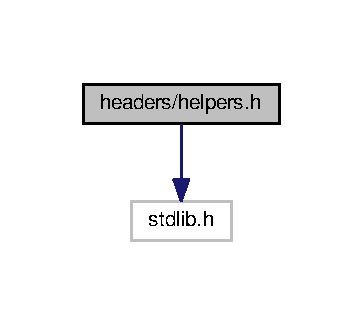
\includegraphics[width=174pt]{helpers_8h__incl}
\end{center}
\end{figure}
This graph shows which files directly or indirectly include this file\+:
\nopagebreak
\begin{figure}[H]
\begin{center}
\leavevmode
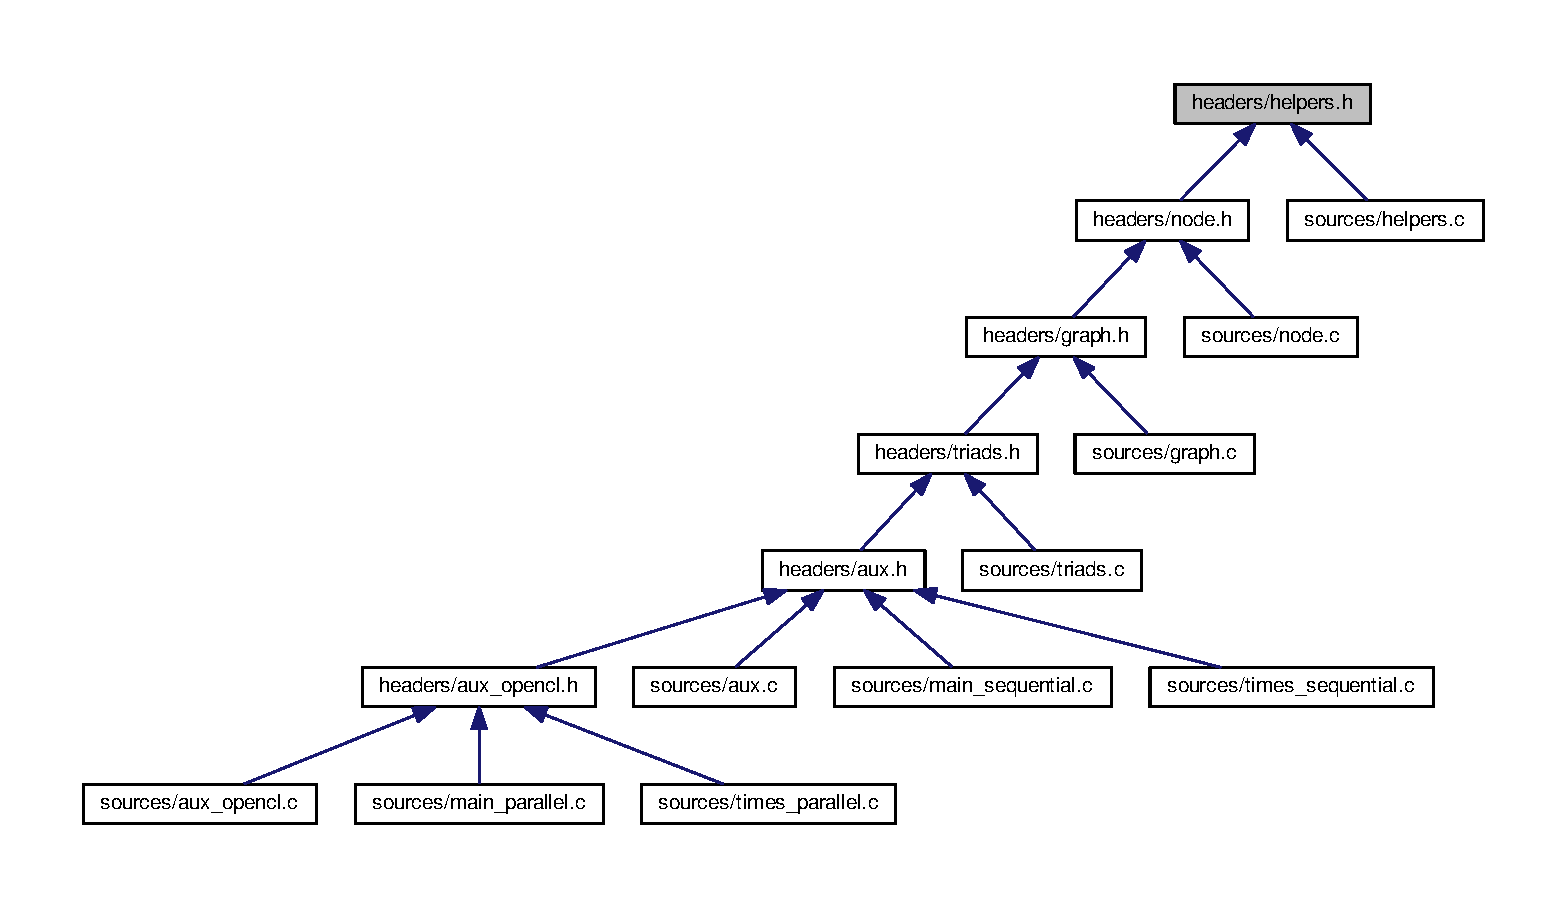
\includegraphics[width=350pt]{helpers_8h__dep__incl}
\end{center}
\end{figure}
\subsection*{Functions}
\begin{DoxyCompactItemize}
\item 
int \hyperlink{helpers_8h_acc35bd25a8a468de5eecd3ac86cad3d6}{linear\+\_\+search} (void $\ast$table, int num\+\_\+elems, size\+\_\+t size, void $\ast$key, int($\ast$comp)(const void $\ast$arg1, const void $\ast$arg2))
\begin{DoxyCompactList}\small\item\em Function that performs linear search over an unordered array. \end{DoxyCompactList}\item 
int \hyperlink{helpers_8h_a179fbd21d334a48da1fb846b53dd04f7}{binary\+\_\+search} (void $\ast$table, int first, int last, size\+\_\+t size, void $\ast$key, int($\ast$comp)(const void $\ast$arg1, const void $\ast$arg2))
\begin{DoxyCompactList}\small\item\em Function that performs binary search over an ordered array. \end{DoxyCompactList}\item 
void \hyperlink{helpers_8h_abf6d4a9fcd1142a7b5bd256d278f8745}{insert\+\_\+sort} (void $\ast$table, size\+\_\+t size, int nmemb, void $\ast$elem, void $\ast$key, int($\ast$comp)(const void $\ast$arg1, const void $\ast$arg2), void($\ast$insert)(void $\ast$table, void $\ast$key, int pos))
\begin{DoxyCompactList}\small\item\em Function that performs the insertion sort (inner loop of the algorithm) \end{DoxyCompactList}\end{DoxyCompactItemize}


\subsection{Detailed Description}
This file contains the definitions of helper functions used used used to search and insert in arrays. ~\newline
In our implementation, we have implemented linear search, binary search and insertion sort algorithms. These are useful for a variety of cases, and thus we decided to implement them in a general way. 

\begin{DoxyAuthor}{Author}
\+: Carlos Alfaro
\end{DoxyAuthor}
\begin{DoxyDate}{Date}
\+: 19-\/10-\/2017 
\end{DoxyDate}


\subsection{Function Documentation}
\mbox{\Hypertarget{helpers_8h_a179fbd21d334a48da1fb846b53dd04f7}\label{helpers_8h_a179fbd21d334a48da1fb846b53dd04f7}} 
\index{helpers.\+h@{helpers.\+h}!binary\+\_\+search@{binary\+\_\+search}}
\index{binary\+\_\+search@{binary\+\_\+search}!helpers.\+h@{helpers.\+h}}
\subsubsection{\texorpdfstring{binary\+\_\+search()}{binary\_search()}}
{\footnotesize\ttfamily int binary\+\_\+search (\begin{DoxyParamCaption}\item[{void $\ast$}]{table,  }\item[{int}]{first,  }\item[{int}]{last,  }\item[{size\+\_\+t}]{size,  }\item[{void $\ast$}]{key,  }\item[{int($\ast$)(const void $\ast$arg1, const void $\ast$arg2)}]{comp }\end{DoxyParamCaption})}



Function that performs binary search over an ordered array. 


\begin{DoxyParams}{Parameters}
{\em void$\ast$} & table\+: The array in which to perform the search \\
\hline
{\em int} & first\+: the first index of the table \\
\hline
{\em int} & last\+: the last index of the table \\
\hline
{\em size\+\_\+t} & size\+: size in bytes of each of the elements of the array \\
\hline
{\em void$\ast$} & key\+: The key to search within the array \\
\hline
{\em int} & ({\itshape comp) (const void} arg1, const void$\ast$ arg2)\+: pointer to the campare function\\
\hline
\end{DoxyParams}
\begin{DoxyReturn}{Returns}
int the position in which the key is stored, if it is found~\newline
 -\/1 otherwise 
\end{DoxyReturn}
\mbox{\Hypertarget{helpers_8h_abf6d4a9fcd1142a7b5bd256d278f8745}\label{helpers_8h_abf6d4a9fcd1142a7b5bd256d278f8745}} 
\index{helpers.\+h@{helpers.\+h}!insert\+\_\+sort@{insert\+\_\+sort}}
\index{insert\+\_\+sort@{insert\+\_\+sort}!helpers.\+h@{helpers.\+h}}
\subsubsection{\texorpdfstring{insert\+\_\+sort()}{insert\_sort()}}
{\footnotesize\ttfamily void insert\+\_\+sort (\begin{DoxyParamCaption}\item[{void $\ast$}]{table,  }\item[{size\+\_\+t}]{size,  }\item[{int}]{nmemb,  }\item[{void $\ast$}]{elem,  }\item[{void $\ast$}]{key,  }\item[{int($\ast$)(const void $\ast$arg1, const void $\ast$arg2)}]{comp,  }\item[{void($\ast$)(void $\ast$table, void $\ast$key, int pos)}]{insert }\end{DoxyParamCaption})}



Function that performs the insertion sort (inner loop of the algorithm) 


\begin{DoxyParams}{Parameters}
{\em void$\ast$} & table\+: The array in which to perform the insertion \\
\hline
{\em size\+\_\+t} & size\+: size in bytes of each of the elements of the array \\
\hline
{\em int} & nmemb\+: Number of elements present in the array \\
\hline
{\em void$\ast$} & elem\+: element to insert \\
\hline
{\em void} & $\ast$key\+: key associated to the element, useful to compare to other elements \\
\hline
{\em int} & ({\itshape comp) (const void} arg1, const void$\ast$ arg2)\+: pointer to the compare function void ({\itshape insert)(void} table, void$\ast$ key, int pos)\+:pointer to the insertion function\\
\hline
\end{DoxyParams}
\begin{DoxyReturn}{Returns}
int the position in which the key is stored, if it is found -\/1 otherwise 
\end{DoxyReturn}
\mbox{\Hypertarget{helpers_8h_acc35bd25a8a468de5eecd3ac86cad3d6}\label{helpers_8h_acc35bd25a8a468de5eecd3ac86cad3d6}} 
\index{helpers.\+h@{helpers.\+h}!linear\+\_\+search@{linear\+\_\+search}}
\index{linear\+\_\+search@{linear\+\_\+search}!helpers.\+h@{helpers.\+h}}
\subsubsection{\texorpdfstring{linear\+\_\+search()}{linear\_search()}}
{\footnotesize\ttfamily int linear\+\_\+search (\begin{DoxyParamCaption}\item[{void $\ast$}]{table,  }\item[{int}]{num\+\_\+elems,  }\item[{size\+\_\+t}]{size,  }\item[{void $\ast$}]{key,  }\item[{int($\ast$)(const void $\ast$arg1, const void $\ast$arg2)}]{comp }\end{DoxyParamCaption})}



Function that performs linear search over an unordered array. 


\begin{DoxyParams}{Parameters}
{\em void$\ast$} & table\+: The array in which to perform the search \\
\hline
{\em int} & num\+\_\+elems\+: Number of elements in the array \\
\hline
{\em size\+\_\+t} & size\+: size in bytes of each of the elements of the array \\
\hline
{\em void$\ast$} & key\+: The key to search within the array \\
\hline
{\em int} & ({\itshape comp) (const void} arg1, const void$\ast$ arg2)\+: pointer to the campare function\\
\hline
\end{DoxyParams}
\begin{DoxyReturn}{Returns}
int the position in which the key is stored, if it is found~\newline
 -\/1 otherwise 
\end{DoxyReturn}

\hypertarget{NDRange__BM__header_8h}{}\section{headers/\+N\+D\+Range\+\_\+\+B\+M\+\_\+header.h File Reference}
\label{NDRange__BM__header_8h}\index{headers/\+N\+D\+Range\+\_\+\+B\+M\+\_\+header.\+h@{headers/\+N\+D\+Range\+\_\+\+B\+M\+\_\+header.\+h}}


This file contains the definitions of the functions needed to execute the N\+D\+Range BM kernels.  


{\ttfamily \#include \char`\"{}defs.\+h\char`\"{}}\newline
Include dependency graph for N\+D\+Range\+\_\+\+B\+M\+\_\+header.\+h\+:\nopagebreak
\begin{figure}[H]
\begin{center}
\leavevmode
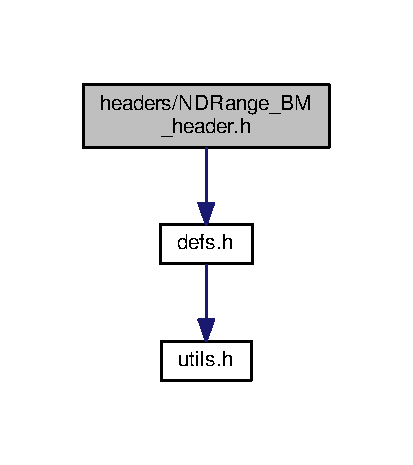
\includegraphics[width=198pt]{NDRange__BM__header_8h__incl}
\end{center}
\end{figure}
\subsection*{Functions}
\begin{DoxyCompactItemize}
\item 
short \hyperlink{NDRange__BM__header_8h_a697625370e04cd92861d106e9f2802d3}{iso\+Tricode} (\+\_\+\+\_\+constant \hyperlink{structEDGE__DEVICE}{E\+D\+G\+E\+\_\+\+D\+E\+V\+I\+CE} $\ast$edges, \hyperlink{structNODE__DEVICE}{N\+O\+D\+E\+\_\+\+D\+E\+V\+I\+CE} $\ast$u, \hyperlink{structNODE__DEVICE}{N\+O\+D\+E\+\_\+\+D\+E\+V\+I\+CE} $\ast$v, unsigned int w\+\_\+id)
\begin{DoxyCompactList}\small\item\em Function that computes the triad type of a triple of nodes. \end{DoxyCompactList}\item 
uint \hyperlink{NDRange__BM__header_8h_a95f02d51d2e478d2203f203da34ca536}{get\+\_\+neighbor\+\_\+id} (\hyperlink{structEDGE__DEVICE}{E\+D\+G\+E\+\_\+\+D\+E\+V\+I\+CE} e)
\begin{DoxyCompactList}\small\item\em Function that returns the neighbor id of an edge. \end{DoxyCompactList}\item 
\hyperlink{utils_8h_aa268a41a13430b18e933ed40207178d0}{D\+I\+R\+E\+C\+T\+I\+ON} \hyperlink{NDRange__BM__header_8h_a3c6ec02b4ab708a4c4cc9d75d8b8bd3d}{get\+\_\+direction} (\hyperlink{structEDGE__DEVICE}{E\+D\+G\+E\+\_\+\+D\+E\+V\+I\+CE} e)
\begin{DoxyCompactList}\small\item\em Function that returns the direction of an edge. \end{DoxyCompactList}\item 
\hyperlink{utils_8h_aa268a41a13430b18e933ed40207178d0}{D\+I\+R\+E\+C\+T\+I\+ON} \hyperlink{NDRange__BM__header_8h_a1c79c56ad87266e0d11764d24f5983d1}{turnup} (\hyperlink{utils_8h_aa268a41a13430b18e933ed40207178d0}{D\+I\+R\+E\+C\+T\+I\+ON} dir)
\begin{DoxyCompactList}\small\item\em Function that turnup the direction of an edge. \end{DoxyCompactList}\item 
int \hyperlink{NDRange__BM__header_8h_a5486ebd7f130983e18b921595f7524ab}{binary\+\_\+search\+\_\+adj\+\_\+list} (\+\_\+\+\_\+constant \hyperlink{structEDGE__DEVICE}{E\+D\+G\+E\+\_\+\+D\+E\+V\+I\+CE} $\ast$table, uint key, int first, int last)
\begin{DoxyCompactList}\small\item\em Function that performs binary search over an ordered array. \end{DoxyCompactList}\item 
int \hyperlink{NDRange__BM__header_8h_a6921fc49ace2c18b2c421c3700ae1d77}{linear\+\_\+search\+\_\+adj\+\_\+list} (\+\_\+\+\_\+constant \hyperlink{structEDGE__DEVICE}{E\+D\+G\+E\+\_\+\+D\+E\+V\+I\+CE} $\ast$table, uint key, uint first, uint last)
\begin{DoxyCompactList}\small\item\em Function that performs linear search over an unordered array. \end{DoxyCompactList}\item 
int \hyperlink{NDRange__BM__header_8h_a3fb99b454cbcec7b11562c474b968a78}{get\+\_\+neighbor\+\_\+pos} (\+\_\+\+\_\+constant \hyperlink{structEDGE__DEVICE}{E\+D\+G\+E\+\_\+\+D\+E\+V\+I\+CE} $\ast$edges, \hyperlink{structNODE__DEVICE}{N\+O\+D\+E\+\_\+\+D\+E\+V\+I\+CE} $\ast$n, unsigned int nid)
\begin{DoxyCompactList}\small\item\em Function that returns the position of a certain neighbor node within the edge array, given the first node and the neighbor id. \end{DoxyCompactList}\item 
\hyperlink{utils_8h_aa268a41a13430b18e933ed40207178d0}{D\+I\+R\+E\+C\+T\+I\+ON} \hyperlink{NDRange__BM__header_8h_a0fd0695a01348883dcb313032684b317}{get\+\_\+dir\+\_\+between\+\_\+nodes} (\+\_\+\+\_\+constant \hyperlink{structEDGE__DEVICE}{E\+D\+G\+E\+\_\+\+D\+E\+V\+I\+CE} $\ast$edges, \hyperlink{structNODE__DEVICE}{N\+O\+D\+E\+\_\+\+D\+E\+V\+I\+CE} $\ast$u, unsigned int v\+\_\+id)
\begin{DoxyCompactList}\small\item\em Function that returns the direction of the edge present between two nodes (u,v) \end{DoxyCompactList}\end{DoxyCompactItemize}


\subsection{Detailed Description}
This file contains the definitions of the functions needed to execute the N\+D\+Range BM kernels. 

\begin{DoxyAuthor}{Author}
\+: Carlos Alfaro
\end{DoxyAuthor}
\begin{DoxyDate}{Date}
\+: 17-\/12-\/2017 
\end{DoxyDate}


\subsection{Function Documentation}
\mbox{\Hypertarget{NDRange__BM__header_8h_a5486ebd7f130983e18b921595f7524ab}\label{NDRange__BM__header_8h_a5486ebd7f130983e18b921595f7524ab}} 
\index{N\+D\+Range\+\_\+\+B\+M\+\_\+header.\+h@{N\+D\+Range\+\_\+\+B\+M\+\_\+header.\+h}!binary\+\_\+search\+\_\+adj\+\_\+list@{binary\+\_\+search\+\_\+adj\+\_\+list}}
\index{binary\+\_\+search\+\_\+adj\+\_\+list@{binary\+\_\+search\+\_\+adj\+\_\+list}!N\+D\+Range\+\_\+\+B\+M\+\_\+header.\+h@{N\+D\+Range\+\_\+\+B\+M\+\_\+header.\+h}}
\subsubsection{\texorpdfstring{binary\+\_\+search\+\_\+adj\+\_\+list()}{binary\_search\_adj\_list()}}
{\footnotesize\ttfamily int binary\+\_\+search\+\_\+adj\+\_\+list (\begin{DoxyParamCaption}\item[{\+\_\+\+\_\+constant \hyperlink{structEDGE__DEVICE}{E\+D\+G\+E\+\_\+\+D\+E\+V\+I\+CE} $\ast$}]{table,  }\item[{uint}]{key,  }\item[{int}]{first,  }\item[{int}]{last }\end{DoxyParamCaption})}



Function that performs binary search over an ordered array. 


\begin{DoxyParams}{Parameters}
{\em \+\_\+\+\_\+constant} & E\+D\+G\+E\+\_\+\+D\+E\+V\+I\+C\+E$\ast$ table\+: The array in which to perform the search \\
\hline
{\em uint} & key\+: The key to search within the array \\
\hline
{\em int} & first\+: the first index of the table \\
\hline
{\em int} & last\+: the last index of the table\\
\hline
\end{DoxyParams}
\begin{DoxyReturn}{Returns}
int the position in which the key is stored, if it is found~\newline
 -\/1 otherwise 
\end{DoxyReturn}
\mbox{\Hypertarget{NDRange__BM__header_8h_a0fd0695a01348883dcb313032684b317}\label{NDRange__BM__header_8h_a0fd0695a01348883dcb313032684b317}} 
\index{N\+D\+Range\+\_\+\+B\+M\+\_\+header.\+h@{N\+D\+Range\+\_\+\+B\+M\+\_\+header.\+h}!get\+\_\+dir\+\_\+between\+\_\+nodes@{get\+\_\+dir\+\_\+between\+\_\+nodes}}
\index{get\+\_\+dir\+\_\+between\+\_\+nodes@{get\+\_\+dir\+\_\+between\+\_\+nodes}!N\+D\+Range\+\_\+\+B\+M\+\_\+header.\+h@{N\+D\+Range\+\_\+\+B\+M\+\_\+header.\+h}}
\subsubsection{\texorpdfstring{get\+\_\+dir\+\_\+between\+\_\+nodes()}{get\_dir\_between\_nodes()}}
{\footnotesize\ttfamily \hyperlink{utils_8h_aa268a41a13430b18e933ed40207178d0}{D\+I\+R\+E\+C\+T\+I\+ON} get\+\_\+dir\+\_\+between\+\_\+nodes (\begin{DoxyParamCaption}\item[{\+\_\+\+\_\+constant \hyperlink{structEDGE__DEVICE}{E\+D\+G\+E\+\_\+\+D\+E\+V\+I\+CE} $\ast$}]{edges,  }\item[{\hyperlink{structNODE__DEVICE}{N\+O\+D\+E\+\_\+\+D\+E\+V\+I\+CE} $\ast$}]{u,  }\item[{unsigned int}]{v\+\_\+id }\end{DoxyParamCaption})}



Function that returns the direction of the edge present between two nodes (u,v) 


\begin{DoxyParams}{Parameters}
{\em \+\_\+\+\_\+constant} & E\+D\+G\+E\+\_\+\+D\+E\+V\+I\+C\+E$\ast$ edges\+: Edge array \\
\hline
{\em N\+O\+D\+E\+\_\+\+D\+E\+V\+I\+C\+E$\ast$} & u\+: The first node \\
\hline
{\em uint} & v\+\_\+id\+: The node id of the second node\\
\hline
\end{DoxyParams}
\begin{DoxyReturn}{Returns}
D\+I\+R\+E\+C\+T\+I\+ON\+: The direction of the edge between the nodes 
\end{DoxyReturn}
\mbox{\Hypertarget{NDRange__BM__header_8h_a3c6ec02b4ab708a4c4cc9d75d8b8bd3d}\label{NDRange__BM__header_8h_a3c6ec02b4ab708a4c4cc9d75d8b8bd3d}} 
\index{N\+D\+Range\+\_\+\+B\+M\+\_\+header.\+h@{N\+D\+Range\+\_\+\+B\+M\+\_\+header.\+h}!get\+\_\+direction@{get\+\_\+direction}}
\index{get\+\_\+direction@{get\+\_\+direction}!N\+D\+Range\+\_\+\+B\+M\+\_\+header.\+h@{N\+D\+Range\+\_\+\+B\+M\+\_\+header.\+h}}
\subsubsection{\texorpdfstring{get\+\_\+direction()}{get\_direction()}}
{\footnotesize\ttfamily \hyperlink{utils_8h_aa268a41a13430b18e933ed40207178d0}{D\+I\+R\+E\+C\+T\+I\+ON} get\+\_\+direction (\begin{DoxyParamCaption}\item[{\hyperlink{structEDGE__DEVICE}{E\+D\+G\+E\+\_\+\+D\+E\+V\+I\+CE}}]{e }\end{DoxyParamCaption})}



Function that returns the direction of an edge. 


\begin{DoxyParams}{Parameters}
{\em \hyperlink{structEDGE__DEVICE}{E\+D\+G\+E\+\_\+\+D\+E\+V\+I\+CE}} & e\+: The edge\\
\hline
\end{DoxyParams}
\begin{DoxyReturn}{Returns}
D\+I\+R\+E\+C\+T\+I\+ON\+: The direction of the edge 
\end{DoxyReturn}
\mbox{\Hypertarget{NDRange__BM__header_8h_a95f02d51d2e478d2203f203da34ca536}\label{NDRange__BM__header_8h_a95f02d51d2e478d2203f203da34ca536}} 
\index{N\+D\+Range\+\_\+\+B\+M\+\_\+header.\+h@{N\+D\+Range\+\_\+\+B\+M\+\_\+header.\+h}!get\+\_\+neighbor\+\_\+id@{get\+\_\+neighbor\+\_\+id}}
\index{get\+\_\+neighbor\+\_\+id@{get\+\_\+neighbor\+\_\+id}!N\+D\+Range\+\_\+\+B\+M\+\_\+header.\+h@{N\+D\+Range\+\_\+\+B\+M\+\_\+header.\+h}}
\subsubsection{\texorpdfstring{get\+\_\+neighbor\+\_\+id()}{get\_neighbor\_id()}}
{\footnotesize\ttfamily uint get\+\_\+neighbor\+\_\+id (\begin{DoxyParamCaption}\item[{\hyperlink{structEDGE__DEVICE}{E\+D\+G\+E\+\_\+\+D\+E\+V\+I\+CE}}]{e }\end{DoxyParamCaption})}



Function that returns the neighbor id of an edge. 


\begin{DoxyParams}{Parameters}
{\em \hyperlink{structEDGE__DEVICE}{E\+D\+G\+E\+\_\+\+D\+E\+V\+I\+CE}} & e\+: The edge\\
\hline
\end{DoxyParams}
\begin{DoxyReturn}{Returns}
uint\+: The neighbor id 
\end{DoxyReturn}
\mbox{\Hypertarget{NDRange__BM__header_8h_a3fb99b454cbcec7b11562c474b968a78}\label{NDRange__BM__header_8h_a3fb99b454cbcec7b11562c474b968a78}} 
\index{N\+D\+Range\+\_\+\+B\+M\+\_\+header.\+h@{N\+D\+Range\+\_\+\+B\+M\+\_\+header.\+h}!get\+\_\+neighbor\+\_\+pos@{get\+\_\+neighbor\+\_\+pos}}
\index{get\+\_\+neighbor\+\_\+pos@{get\+\_\+neighbor\+\_\+pos}!N\+D\+Range\+\_\+\+B\+M\+\_\+header.\+h@{N\+D\+Range\+\_\+\+B\+M\+\_\+header.\+h}}
\subsubsection{\texorpdfstring{get\+\_\+neighbor\+\_\+pos()}{get\_neighbor\_pos()}}
{\footnotesize\ttfamily int get\+\_\+neighbor\+\_\+pos (\begin{DoxyParamCaption}\item[{\+\_\+\+\_\+constant \hyperlink{structEDGE__DEVICE}{E\+D\+G\+E\+\_\+\+D\+E\+V\+I\+CE} $\ast$}]{edges,  }\item[{\hyperlink{structNODE__DEVICE}{N\+O\+D\+E\+\_\+\+D\+E\+V\+I\+CE} $\ast$}]{n,  }\item[{unsigned int}]{nid }\end{DoxyParamCaption})}



Function that returns the position of a certain neighbor node within the edge array, given the first node and the neighbor id. 


\begin{DoxyParams}{Parameters}
{\em \+\_\+\+\_\+constant} & E\+D\+G\+E\+\_\+\+D\+E\+V\+I\+C\+E$\ast$ edges\+: Edge array in which to search \\
\hline
{\em N\+O\+D\+E\+\_\+\+D\+E\+V\+I\+C\+E$\ast$} & n\+: The node of which we want to get the neighbor position \\
\hline
{\em uint} & nid\+: The node id of the neighbor we want to search\\
\hline
\end{DoxyParams}
\begin{DoxyReturn}{Returns}
int\+: The position within the edge array 
\end{DoxyReturn}
\mbox{\Hypertarget{NDRange__BM__header_8h_a697625370e04cd92861d106e9f2802d3}\label{NDRange__BM__header_8h_a697625370e04cd92861d106e9f2802d3}} 
\index{N\+D\+Range\+\_\+\+B\+M\+\_\+header.\+h@{N\+D\+Range\+\_\+\+B\+M\+\_\+header.\+h}!iso\+Tricode@{iso\+Tricode}}
\index{iso\+Tricode@{iso\+Tricode}!N\+D\+Range\+\_\+\+B\+M\+\_\+header.\+h@{N\+D\+Range\+\_\+\+B\+M\+\_\+header.\+h}}
\subsubsection{\texorpdfstring{iso\+Tricode()}{isoTricode()}}
{\footnotesize\ttfamily short iso\+Tricode (\begin{DoxyParamCaption}\item[{\+\_\+\+\_\+constant \hyperlink{structEDGE__DEVICE}{E\+D\+G\+E\+\_\+\+D\+E\+V\+I\+CE} $\ast$}]{edges,  }\item[{\hyperlink{structNODE__DEVICE}{N\+O\+D\+E\+\_\+\+D\+E\+V\+I\+CE} $\ast$}]{u,  }\item[{\hyperlink{structNODE__DEVICE}{N\+O\+D\+E\+\_\+\+D\+E\+V\+I\+CE} $\ast$}]{v,  }\item[{unsigned int}]{w\+\_\+id }\end{DoxyParamCaption})}



Function that computes the triad type of a triple of nodes. 


\begin{DoxyParams}{Parameters}
{\em \+\_\+\+\_\+constant} & E\+D\+G\+E\+\_\+\+D\+E\+V\+I\+C\+E$\ast$ edges\+: Global edge array \\
\hline
{\em N\+O\+D\+E\+\_\+\+D\+E\+V\+I\+C\+E$\ast$} & u\+: First node of the triple \\
\hline
{\em N\+O\+D\+E\+\_\+\+D\+E\+V\+I\+C\+E$\ast$} & v\+: Second node of the triple \\
\hline
{\em uint} & w\+\_\+id\+: Id of the third node of the triple\\
\hline
\end{DoxyParams}
\begin{DoxyReturn}{Returns}
int\+: A number between 0 and 15, depending on the configuration of the triple 
\end{DoxyReturn}
\mbox{\Hypertarget{NDRange__BM__header_8h_a6921fc49ace2c18b2c421c3700ae1d77}\label{NDRange__BM__header_8h_a6921fc49ace2c18b2c421c3700ae1d77}} 
\index{N\+D\+Range\+\_\+\+B\+M\+\_\+header.\+h@{N\+D\+Range\+\_\+\+B\+M\+\_\+header.\+h}!linear\+\_\+search\+\_\+adj\+\_\+list@{linear\+\_\+search\+\_\+adj\+\_\+list}}
\index{linear\+\_\+search\+\_\+adj\+\_\+list@{linear\+\_\+search\+\_\+adj\+\_\+list}!N\+D\+Range\+\_\+\+B\+M\+\_\+header.\+h@{N\+D\+Range\+\_\+\+B\+M\+\_\+header.\+h}}
\subsubsection{\texorpdfstring{linear\+\_\+search\+\_\+adj\+\_\+list()}{linear\_search\_adj\_list()}}
{\footnotesize\ttfamily int linear\+\_\+search\+\_\+adj\+\_\+list (\begin{DoxyParamCaption}\item[{\+\_\+\+\_\+constant \hyperlink{structEDGE__DEVICE}{E\+D\+G\+E\+\_\+\+D\+E\+V\+I\+CE} $\ast$}]{table,  }\item[{uint}]{key,  }\item[{uint}]{first,  }\item[{uint}]{last }\end{DoxyParamCaption})}



Function that performs linear search over an unordered array. 


\begin{DoxyParams}{Parameters}
{\em \+\_\+\+\_\+constant} & E\+D\+G\+E\+\_\+\+D\+E\+V\+I\+C\+E$\ast$ table\+: The array in which to perform the search \\
\hline
{\em uint} & key\+: The key to search within the array \\
\hline
{\em int} & first\+: the first index of the table \\
\hline
{\em int} & last\+: the last index of the table\\
\hline
\end{DoxyParams}
\begin{DoxyReturn}{Returns}
int the position in which the key is stored, if it is found~\newline
 -\/1 otherwise 
\end{DoxyReturn}
\mbox{\Hypertarget{NDRange__BM__header_8h_a1c79c56ad87266e0d11764d24f5983d1}\label{NDRange__BM__header_8h_a1c79c56ad87266e0d11764d24f5983d1}} 
\index{N\+D\+Range\+\_\+\+B\+M\+\_\+header.\+h@{N\+D\+Range\+\_\+\+B\+M\+\_\+header.\+h}!turnup@{turnup}}
\index{turnup@{turnup}!N\+D\+Range\+\_\+\+B\+M\+\_\+header.\+h@{N\+D\+Range\+\_\+\+B\+M\+\_\+header.\+h}}
\subsubsection{\texorpdfstring{turnup()}{turnup()}}
{\footnotesize\ttfamily \hyperlink{utils_8h_aa268a41a13430b18e933ed40207178d0}{D\+I\+R\+E\+C\+T\+I\+ON} turnup (\begin{DoxyParamCaption}\item[{\hyperlink{utils_8h_aa268a41a13430b18e933ed40207178d0}{D\+I\+R\+E\+C\+T\+I\+ON}}]{dir }\end{DoxyParamCaption})}



Function that turnup the direction of an edge. 


\begin{DoxyParams}{Parameters}
{\em D\+I\+R\+E\+C\+T\+I\+ON} & dir\+: The direction to turnup\\
\hline
\end{DoxyParams}
\begin{DoxyReturn}{Returns}
D\+I\+R\+E\+C\+T\+I\+ON\+: The opposite direction 
\end{DoxyReturn}

\hypertarget{node_8h}{}\section{headers/node.h File Reference}
\label{node_8h}\index{headers/node.\+h@{headers/node.\+h}}


This file contains the definitions of the functions ~\newline
needed to create and manage a node of a graph. ~\newline
In our implementation, the graph is basically a list of nodes ~\newline
which are identified uniquely with and unsigned integer. Each ~\newline
node keeps track of its adjacency list, bi means of an array of ~\newline
edges. Since each edge connects two nodes, edge information will ~\newline
be duplicated.  


{\ttfamily \#include \char`\"{}edge.\+h\char`\"{}}\newline
{\ttfamily \#include \char`\"{}helpers.\+h\char`\"{}}\newline
Include dependency graph for node.\+h\+:\nopagebreak
\begin{figure}[H]
\begin{center}
\leavevmode
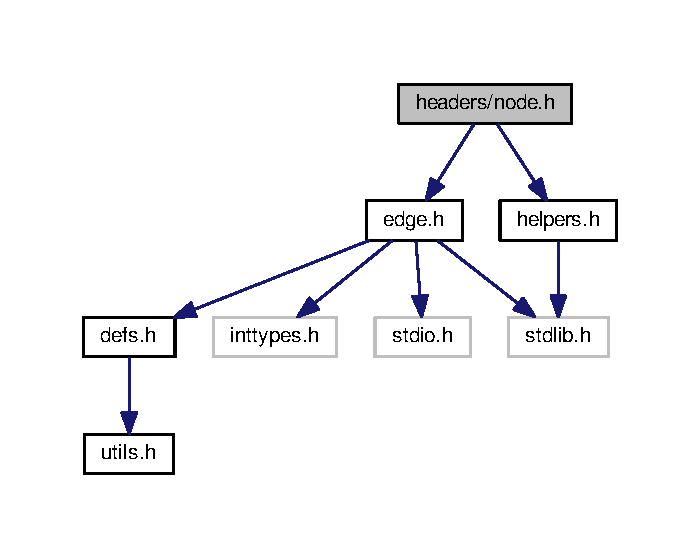
\includegraphics[width=336pt]{node_8h__incl}
\end{center}
\end{figure}
This graph shows which files directly or indirectly include this file\+:\nopagebreak
\begin{figure}[H]
\begin{center}
\leavevmode
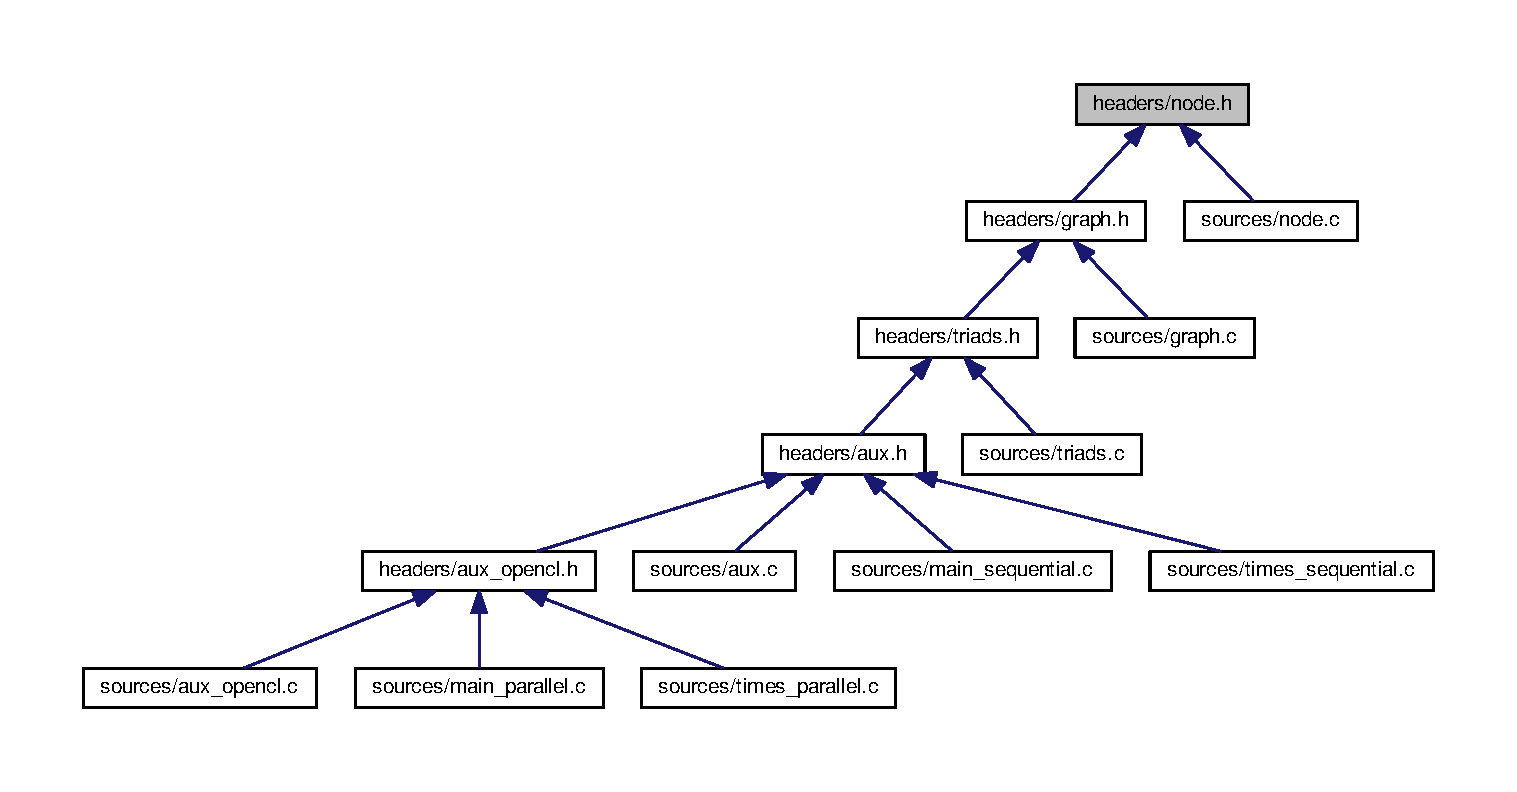
\includegraphics[width=192pt]{node_8h__dep__incl}
\end{center}
\end{figure}
\subsection*{Data Structures}
\begin{DoxyCompactItemize}
\item 
struct \hyperlink{structNODE}{N\+O\+DE}
\begin{DoxyCompactList}\small\item\em This structure stores the information of a node of the graph. \end{DoxyCompactList}\end{DoxyCompactItemize}
\subsection*{Functions}
\begin{DoxyCompactItemize}
\item 
\hyperlink{structNODE}{N\+O\+DE} $\ast$ \hyperlink{node_8h_a44b280e18f7f2ff59e126501cb5da4cf}{create\+\_\+node} (uint32\+\_\+t node\+\_\+id)
\begin{DoxyCompactList}\small\item\em Function that creates a new node, allocating memory for its fields and initializing them. The node\+\_\+id is set to the parameter passed, while the adj\+\_\+list is set to N\+U\+LL and the num\+\_\+neighbors is set to 0. \end{DoxyCompactList}\item 
\hyperlink{utils_8h_a32c27cc471df37f4fc818d65de0a56c4}{S\+T\+A\+T\+US} \hyperlink{node_8h_a67c0e1812fc9ef4b2f1f2760cfbc6ac5}{add\+\_\+edge\+\_\+to\+\_\+node} (\hyperlink{structNODE}{N\+O\+DE} $\ast$n, uint32\+\_\+t neighbor\+\_\+id, \hyperlink{utils_8h_aa268a41a13430b18e933ed40207178d0}{D\+I\+R\+E\+C\+T\+I\+ON} dir)
\begin{DoxyCompactList}\small\item\em Function that creates a new node, allocating memory for its fields and initializing them. The node\+\_\+id is set to the parameter passed, while the adj\+\_\+list is set to N\+U\+LL and the num\+\_\+neighbors is set to 0. \end{DoxyCompactList}\item 
int \hyperlink{node_8h_a5b0769e751658fc3d9768c079ecba12c}{get\+\_\+neighbor\+\_\+pos} (\hyperlink{structNODE}{N\+O\+DE} $\ast$n, uint32\+\_\+t neighbor\+\_\+id)
\begin{DoxyCompactList}\small\item\em Function that returns the position of a certain noighbor node within the adjacency list of the node, given the neighbor id. \end{DoxyCompactList}\item 
uint32\+\_\+t \hyperlink{node_8h_aed1bcaeca3d8358924632d6cf06dd29e}{get\+\_\+node\+\_\+id} (\hyperlink{structNODE}{N\+O\+DE} $\ast$n)
\begin{DoxyCompactList}\small\item\em Function that returns id of a certain node. \end{DoxyCompactList}\item 
\hyperlink{edge_8h_ab4a642fc78a44ca8df119570b3288e13}{E\+D\+GE} \hyperlink{node_8h_a1f56c95c3bf68181e75cef1e8a4ff2fc}{get\+\_\+edge} (\hyperlink{structNODE}{N\+O\+DE} $\ast$n, int pos)
\begin{DoxyCompactList}\small\item\em Function that the edge present in a certain position~\newline
of the adjacency list of a node. \end{DoxyCompactList}\item 
\hyperlink{edge_8h_ab4a642fc78a44ca8df119570b3288e13}{E\+D\+GE} $\ast$ \hyperlink{node_8h_a304e4f1cf8e0dbadd842ac4c8336c9f1}{get\+\_\+adj\+\_\+list} (\hyperlink{structNODE}{N\+O\+DE} $\ast$n)
\begin{DoxyCompactList}\small\item\em Function that returns the adjacency list of a certain node. \end{DoxyCompactList}\item 
int \hyperlink{node_8h_a02799b8fad8a4f676a9a6d5d0b82c366}{get\+\_\+num\+\_\+neighbors} (\hyperlink{structNODE}{N\+O\+DE} $\ast$n)
\begin{DoxyCompactList}\small\item\em Function that returns the number of neighbors a certain node has. \end{DoxyCompactList}\item 
int \hyperlink{node_8h_a6c59974e491a07d3c328570d42c3dbdb}{get\+\_\+degree} (\hyperlink{structNODE}{N\+O\+DE} $\ast$n)
\begin{DoxyCompactList}\small\item\em Function that returns the degree of a certain node. \end{DoxyCompactList}\item 
int \hyperlink{node_8h_aab41692fa3f3d5214a5dadb4f616a853}{comp\+\_\+nodes\+\_\+by\+\_\+id} (const void $\ast$key, const void $\ast$pnode)
\begin{DoxyCompactList}\small\item\em Function that compares two nodes (useful for binary search and insertion sort).~\newline
The comparison is made based on the node ids. \end{DoxyCompactList}\item 
int \hyperlink{node_8h_ac2c976ce0d52406c4df50195371276b8}{comp\+\_\+nodes\+\_\+by\+\_\+degree} (const void $\ast$key, const void $\ast$pnode)
\begin{DoxyCompactList}\small\item\em Function that compares two nodes (useful for binary search and insertion sort).~\newline
The comparison is made based on the number of neighbors of each node. \end{DoxyCompactList}\item 
int \hyperlink{node_8h_ab797719885a33013788cb2d4b248a36e}{comp\+\_\+ids} (const void $\ast$key, const void $\ast$pid)
\begin{DoxyCompactList}\small\item\em Function that compares two ids (useful for binary search and insertion sort). \end{DoxyCompactList}\item 
void \hyperlink{node_8h_abd4c035d081c773dff95d4f62a781ef6}{insert\+\_\+nodes} (void $\ast$nodes, void $\ast$node, int pos)
\begin{DoxyCompactList}\small\item\em Function that inserts a node in a list for nodes ~\newline
(useful for the helper function insert\+\_\+sort) \end{DoxyCompactList}\item 
uint32\+\_\+t $\ast$ \hyperlink{node_8h_af2840bd87ae7f23b8f0416f47ddb67da}{union\+\_\+adj\+\_\+lists\+\_\+ordered} (int $\ast$card\+\_\+S, \hyperlink{structNODE}{N\+O\+DE} $\ast$u, \hyperlink{structNODE}{N\+O\+DE} $\ast$v)
\begin{DoxyCompactList}\small\item\em Function that constructs the ordered union of the adjacency lists of two nodes ~\newline
 u and v, storing only the neighbor ids and avoiding the insertion of ~\newline
 u and v (in case they were present in the lists).~\newline
 The function also fills the parameter card\+\_\+S with the cardinality of the ~\newline
 union. \end{DoxyCompactList}\item 
uint32\+\_\+t $\ast$ \hyperlink{node_8h_a9bef0eea3e19f9545e070374f5abc055}{union\+\_\+adj\+\_\+lists\+\_\+not\+\_\+ordered} (int $\ast$card\+\_\+S, \hyperlink{structNODE}{N\+O\+DE} $\ast$u, \hyperlink{structNODE}{N\+O\+DE} $\ast$v)
\begin{DoxyCompactList}\small\item\em Function that constructs the not ordered union of the adjacency lists of two nodes ~\newline
 u and v, storing only the neighbor ids and avoiding the insertion of ~\newline
 u and v (in case they were present in the lists).~\newline
 The function also fills the parameter card\+\_\+S with the cardinality of the~\newline
 union. \end{DoxyCompactList}\item 
\hyperlink{utils_8h_aa268a41a13430b18e933ed40207178d0}{D\+I\+R\+E\+C\+T\+I\+ON} \hyperlink{node_8h_acfeda132522226efe0dcab8ff2813da3}{get\+\_\+dir\+\_\+between\+\_\+nodes} (\hyperlink{structNODE}{N\+O\+DE} $\ast$u, \hyperlink{structNODE}{N\+O\+DE} $\ast$v)
\begin{DoxyCompactList}\small\item\em Function that constructs the union of the adjacency lists of two nodes~\newline
 u and v, storing only the neighbor ids and avoiding the insertion of ~\newline
 u and v (in case they were present in the lists).~\newline
 The function also fills the parameter card\+\_\+S with the cardinality of the~\newline
 union. \end{DoxyCompactList}\item 
\hyperlink{utils_8h_a3e5b8192e7d9ffaf3542f1210aec18dd}{B\+O\+OL} \hyperlink{node_8h_a37de73278d193b74aed6a86833cb8c87}{not\+\_\+connected} (\hyperlink{structNODE}{N\+O\+DE} $\ast$u, \hyperlink{structNODE}{N\+O\+DE} $\ast$v)
\begin{DoxyCompactList}\small\item\em Function that checks if two nodes u and v are connected. \end{DoxyCompactList}\item 
void \hyperlink{node_8h_ac537b7cd330634c71ec43a4ce258c3b1}{print\+\_\+node} (\hyperlink{structNODE}{N\+O\+DE} $\ast$n)
\begin{DoxyCompactList}\small\item\em Function that prints the information of a node. \end{DoxyCompactList}\item 
void \hyperlink{node_8h_a3f5e6b88f2394c03ffa21bd8e4bdb9c0}{destroy\+\_\+node} (\hyperlink{structNODE}{N\+O\+DE} $\ast$n)
\begin{DoxyCompactList}\small\item\em Function that destroys a node, freeing the memory of ~\newline
 its structures. \end{DoxyCompactList}\end{DoxyCompactItemize}


\subsection{Detailed Description}
This file contains the definitions of the functions ~\newline
needed to create and manage a node of a graph. ~\newline
In our implementation, the graph is basically a list of nodes ~\newline
which are identified uniquely with and unsigned integer. Each ~\newline
node keeps track of its adjacency list, bi means of an array of ~\newline
edges. Since each edge connects two nodes, edge information will ~\newline
be duplicated. 

\begin{DoxyAuthor}{Author}
\+: Carlos Alfaro
\end{DoxyAuthor}
\begin{DoxyDate}{Date}
\+: 23-\/10-\/2017 
\end{DoxyDate}


\subsection{Function Documentation}
\mbox{\Hypertarget{node_8h_a67c0e1812fc9ef4b2f1f2760cfbc6ac5}\label{node_8h_a67c0e1812fc9ef4b2f1f2760cfbc6ac5}} 
\index{node.\+h@{node.\+h}!add\+\_\+edge\+\_\+to\+\_\+node@{add\+\_\+edge\+\_\+to\+\_\+node}}
\index{add\+\_\+edge\+\_\+to\+\_\+node@{add\+\_\+edge\+\_\+to\+\_\+node}!node.\+h@{node.\+h}}
\subsubsection{\texorpdfstring{add\+\_\+edge\+\_\+to\+\_\+node()}{add\_edge\_to\_node()}}
{\footnotesize\ttfamily \hyperlink{utils_8h_a32c27cc471df37f4fc818d65de0a56c4}{S\+T\+A\+T\+US} add\+\_\+edge\+\_\+to\+\_\+node (\begin{DoxyParamCaption}\item[{\hyperlink{structNODE}{N\+O\+DE} $\ast$}]{n,  }\item[{uint32\+\_\+t}]{neighbor\+\_\+id,  }\item[{\hyperlink{utils_8h_aa268a41a13430b18e933ed40207178d0}{D\+I\+R\+E\+C\+T\+I\+ON}}]{dir }\end{DoxyParamCaption})}



Function that creates a new node, allocating memory for its fields and initializing them. The node\+\_\+id is set to the parameter passed, while the adj\+\_\+list is set to N\+U\+LL and the num\+\_\+neighbors is set to 0. 


\begin{DoxyParams}{Parameters}
{\em N\+O\+D\+E$\ast$} & n\+: The node in which we want to insert the edge \\
\hline
{\em uint32\+\_\+t} & neighbor\+\_\+id\+: The node id of the neighbor we want to insert \\
\hline
{\em D\+I\+R\+E\+C\+T\+I\+ON} & dir\+: The direction of the edge we want to insert\\
\hline
\end{DoxyParams}
\begin{DoxyReturn}{Returns}
S\+T\+A\+T\+US\+: OK if the insertion was successful E\+RR otherwise 
\end{DoxyReturn}
\mbox{\Hypertarget{node_8h_ab797719885a33013788cb2d4b248a36e}\label{node_8h_ab797719885a33013788cb2d4b248a36e}} 
\index{node.\+h@{node.\+h}!comp\+\_\+ids@{comp\+\_\+ids}}
\index{comp\+\_\+ids@{comp\+\_\+ids}!node.\+h@{node.\+h}}
\subsubsection{\texorpdfstring{comp\+\_\+ids()}{comp\_ids()}}
{\footnotesize\ttfamily int comp\+\_\+ids (\begin{DoxyParamCaption}\item[{const void $\ast$}]{key,  }\item[{const void $\ast$}]{pid }\end{DoxyParamCaption})}



Function that compares two ids (useful for binary search and insertion sort). 


\begin{DoxyParams}{Parameters}
{\em const} & void$\ast$ key\+: The key we want to compare to the pointer. It is a pointer an id. \\
\hline
{\em const} & void$\ast$ pid\+: A pointer to the id we want to compare to the key\\
\hline
\end{DoxyParams}
\begin{DoxyReturn}{Returns}
int A number that is less than, greater than or equal to 0, depending on weather the key is less than, greather than or equal to the id. 
\end{DoxyReturn}
\mbox{\Hypertarget{node_8h_ac2c976ce0d52406c4df50195371276b8}\label{node_8h_ac2c976ce0d52406c4df50195371276b8}} 
\index{node.\+h@{node.\+h}!comp\+\_\+nodes\+\_\+by\+\_\+degree@{comp\+\_\+nodes\+\_\+by\+\_\+degree}}
\index{comp\+\_\+nodes\+\_\+by\+\_\+degree@{comp\+\_\+nodes\+\_\+by\+\_\+degree}!node.\+h@{node.\+h}}
\subsubsection{\texorpdfstring{comp\+\_\+nodes\+\_\+by\+\_\+degree()}{comp\_nodes\_by\_degree()}}
{\footnotesize\ttfamily int comp\+\_\+nodes\+\_\+by\+\_\+degree (\begin{DoxyParamCaption}\item[{const void $\ast$}]{key,  }\item[{const void $\ast$}]{pnode }\end{DoxyParamCaption})}



Function that compares two nodes (useful for binary search and insertion sort).~\newline
The comparison is made based on the number of neighbors of each node. 


\begin{DoxyParams}{Parameters}
{\em const} & void$\ast$ key\+: The key we want to compare to the other node. It is a pointer to the number of neighbors of a node. \\
\hline
{\em const} & void$\ast$ pnode\+: A pointer to the node we want to compare to the key\\
\hline
\end{DoxyParams}
\begin{DoxyReturn}{Returns}
int A number that is less than, greater than or equal to 0, depending on weather the key is less than, greather than or equal to the pnode. 
\end{DoxyReturn}
\mbox{\Hypertarget{node_8h_aab41692fa3f3d5214a5dadb4f616a853}\label{node_8h_aab41692fa3f3d5214a5dadb4f616a853}} 
\index{node.\+h@{node.\+h}!comp\+\_\+nodes\+\_\+by\+\_\+id@{comp\+\_\+nodes\+\_\+by\+\_\+id}}
\index{comp\+\_\+nodes\+\_\+by\+\_\+id@{comp\+\_\+nodes\+\_\+by\+\_\+id}!node.\+h@{node.\+h}}
\subsubsection{\texorpdfstring{comp\+\_\+nodes\+\_\+by\+\_\+id()}{comp\_nodes\_by\_id()}}
{\footnotesize\ttfamily int comp\+\_\+nodes\+\_\+by\+\_\+id (\begin{DoxyParamCaption}\item[{const void $\ast$}]{key,  }\item[{const void $\ast$}]{pnode }\end{DoxyParamCaption})}



Function that compares two nodes (useful for binary search and insertion sort).~\newline
The comparison is made based on the node ids. 


\begin{DoxyParams}{Parameters}
{\em const} & void$\ast$ key\+: The key we want to compare to the other node. It is a pointer to a node id. \\
\hline
{\em const} & void$\ast$ pnode\+: A pointer to the node we want to compare to the key\\
\hline
\end{DoxyParams}
\begin{DoxyReturn}{Returns}
int A number that is less than, greater than or equal to 0, depending on weather the key is less than, greather than or equal to the pnode. 
\end{DoxyReturn}
\mbox{\Hypertarget{node_8h_a44b280e18f7f2ff59e126501cb5da4cf}\label{node_8h_a44b280e18f7f2ff59e126501cb5da4cf}} 
\index{node.\+h@{node.\+h}!create\+\_\+node@{create\+\_\+node}}
\index{create\+\_\+node@{create\+\_\+node}!node.\+h@{node.\+h}}
\subsubsection{\texorpdfstring{create\+\_\+node()}{create\_node()}}
{\footnotesize\ttfamily \hyperlink{structNODE}{N\+O\+DE}$\ast$ create\+\_\+node (\begin{DoxyParamCaption}\item[{uint32\+\_\+t}]{node\+\_\+id }\end{DoxyParamCaption})}



Function that creates a new node, allocating memory for its fields and initializing them. The node\+\_\+id is set to the parameter passed, while the adj\+\_\+list is set to N\+U\+LL and the num\+\_\+neighbors is set to 0. 


\begin{DoxyParams}{Parameters}
{\em uint32\+\_\+t} & node\+\_\+id\+: The id of the node\\
\hline
\end{DoxyParams}
\begin{DoxyReturn}{Returns}
N\+O\+D\+E$\ast$\+: A pointer to the node just created. 
\end{DoxyReturn}
\mbox{\Hypertarget{node_8h_a3f5e6b88f2394c03ffa21bd8e4bdb9c0}\label{node_8h_a3f5e6b88f2394c03ffa21bd8e4bdb9c0}} 
\index{node.\+h@{node.\+h}!destroy\+\_\+node@{destroy\+\_\+node}}
\index{destroy\+\_\+node@{destroy\+\_\+node}!node.\+h@{node.\+h}}
\subsubsection{\texorpdfstring{destroy\+\_\+node()}{destroy\_node()}}
{\footnotesize\ttfamily void destroy\+\_\+node (\begin{DoxyParamCaption}\item[{\hyperlink{structNODE}{N\+O\+DE} $\ast$}]{n }\end{DoxyParamCaption})}



Function that destroys a node, freeing the memory of ~\newline
 its structures. 


\begin{DoxyParams}{Parameters}
{\em N\+O\+D\+E$\ast$} & n\+: the node to destroy\\
\hline
\end{DoxyParams}
\begin{DoxyReturn}{Returns}
none 
\end{DoxyReturn}
\mbox{\Hypertarget{node_8h_a304e4f1cf8e0dbadd842ac4c8336c9f1}\label{node_8h_a304e4f1cf8e0dbadd842ac4c8336c9f1}} 
\index{node.\+h@{node.\+h}!get\+\_\+adj\+\_\+list@{get\+\_\+adj\+\_\+list}}
\index{get\+\_\+adj\+\_\+list@{get\+\_\+adj\+\_\+list}!node.\+h@{node.\+h}}
\subsubsection{\texorpdfstring{get\+\_\+adj\+\_\+list()}{get\_adj\_list()}}
{\footnotesize\ttfamily \hyperlink{edge_8h_ab4a642fc78a44ca8df119570b3288e13}{E\+D\+GE}$\ast$ get\+\_\+adj\+\_\+list (\begin{DoxyParamCaption}\item[{\hyperlink{structNODE}{N\+O\+DE} $\ast$}]{n }\end{DoxyParamCaption})}



Function that returns the adjacency list of a certain node. 


\begin{DoxyParams}{Parameters}
{\em N\+O\+D\+E$\ast$} & n\+: The node of which we want to get the adjacency list\\
\hline
\end{DoxyParams}
\begin{DoxyReturn}{Returns}
E\+D\+G\+E$\ast$\+: The adjacency list 
\end{DoxyReturn}
\mbox{\Hypertarget{node_8h_a6c59974e491a07d3c328570d42c3dbdb}\label{node_8h_a6c59974e491a07d3c328570d42c3dbdb}} 
\index{node.\+h@{node.\+h}!get\+\_\+degree@{get\+\_\+degree}}
\index{get\+\_\+degree@{get\+\_\+degree}!node.\+h@{node.\+h}}
\subsubsection{\texorpdfstring{get\+\_\+degree()}{get\_degree()}}
{\footnotesize\ttfamily int get\+\_\+degree (\begin{DoxyParamCaption}\item[{\hyperlink{structNODE}{N\+O\+DE} $\ast$}]{n }\end{DoxyParamCaption})}



Function that returns the degree of a certain node. 


\begin{DoxyParams}{Parameters}
{\em N\+O\+D\+E$\ast$} & n\+: The node of which we want to discover the degree\\
\hline
\end{DoxyParams}
\begin{DoxyReturn}{Returns}
int the degree 
\end{DoxyReturn}
\mbox{\Hypertarget{node_8h_acfeda132522226efe0dcab8ff2813da3}\label{node_8h_acfeda132522226efe0dcab8ff2813da3}} 
\index{node.\+h@{node.\+h}!get\+\_\+dir\+\_\+between\+\_\+nodes@{get\+\_\+dir\+\_\+between\+\_\+nodes}}
\index{get\+\_\+dir\+\_\+between\+\_\+nodes@{get\+\_\+dir\+\_\+between\+\_\+nodes}!node.\+h@{node.\+h}}
\subsubsection{\texorpdfstring{get\+\_\+dir\+\_\+between\+\_\+nodes()}{get\_dir\_between\_nodes()}}
{\footnotesize\ttfamily \hyperlink{utils_8h_aa268a41a13430b18e933ed40207178d0}{D\+I\+R\+E\+C\+T\+I\+ON} get\+\_\+dir\+\_\+between\+\_\+nodes (\begin{DoxyParamCaption}\item[{\hyperlink{structNODE}{N\+O\+DE} $\ast$}]{u,  }\item[{\hyperlink{structNODE}{N\+O\+DE} $\ast$}]{v }\end{DoxyParamCaption})}



Function that constructs the union of the adjacency lists of two nodes~\newline
 u and v, storing only the neighbor ids and avoiding the insertion of ~\newline
 u and v (in case they were present in the lists).~\newline
 The function also fills the parameter card\+\_\+S with the cardinality of the~\newline
 union. 


\begin{DoxyParams}{Parameters}
{\em N\+O\+D\+E$\ast$} & u\+: The first node \\
\hline
{\em N\+O\+D\+E$\ast$} & v\+: The second node\\
\hline
\end{DoxyParams}
\begin{DoxyReturn}{Returns}
D\+I\+R\+E\+C\+T\+I\+ON\+: The direction between the two nodes\+:~\newline
 I\+N\+\_\+\+O\+UT, O\+U\+T\+\_\+\+IN, or B\+I\+D\+I\+R\+E\+C\+T\+I\+O\+N\+AL in case they are connected.~\newline
 N\+O\+NE in case they are not connected 
\end{DoxyReturn}
\mbox{\Hypertarget{node_8h_a1f56c95c3bf68181e75cef1e8a4ff2fc}\label{node_8h_a1f56c95c3bf68181e75cef1e8a4ff2fc}} 
\index{node.\+h@{node.\+h}!get\+\_\+edge@{get\+\_\+edge}}
\index{get\+\_\+edge@{get\+\_\+edge}!node.\+h@{node.\+h}}
\subsubsection{\texorpdfstring{get\+\_\+edge()}{get\_edge()}}
{\footnotesize\ttfamily \hyperlink{edge_8h_ab4a642fc78a44ca8df119570b3288e13}{E\+D\+GE} get\+\_\+edge (\begin{DoxyParamCaption}\item[{\hyperlink{structNODE}{N\+O\+DE} $\ast$}]{n,  }\item[{int}]{pos }\end{DoxyParamCaption})}



Function that the edge present in a certain position~\newline
of the adjacency list of a node. 


\begin{DoxyParams}{Parameters}
{\em N\+O\+D\+E$\ast$} & n\+: The node from which we want to get the edge \\
\hline
{\em int} & pos\+: The position within the adjacency list\\
\hline
\end{DoxyParams}
\begin{DoxyReturn}{Returns}
E\+D\+GE\+: the edge 
\end{DoxyReturn}
\mbox{\Hypertarget{node_8h_a5b0769e751658fc3d9768c079ecba12c}\label{node_8h_a5b0769e751658fc3d9768c079ecba12c}} 
\index{node.\+h@{node.\+h}!get\+\_\+neighbor\+\_\+pos@{get\+\_\+neighbor\+\_\+pos}}
\index{get\+\_\+neighbor\+\_\+pos@{get\+\_\+neighbor\+\_\+pos}!node.\+h@{node.\+h}}
\subsubsection{\texorpdfstring{get\+\_\+neighbor\+\_\+pos()}{get\_neighbor\_pos()}}
{\footnotesize\ttfamily int get\+\_\+neighbor\+\_\+pos (\begin{DoxyParamCaption}\item[{\hyperlink{structNODE}{N\+O\+DE} $\ast$}]{n,  }\item[{uint32\+\_\+t}]{neighbor\+\_\+id }\end{DoxyParamCaption})}



Function that returns the position of a certain noighbor node within the adjacency list of the node, given the neighbor id. 

Getter functions 
\begin{DoxyParams}{Parameters}
{\em N\+O\+D\+E$\ast$} & n\+: The node of which we want to get the neighbor position \\
\hline
{\em uint32\+\_\+t} & neighbor\+\_\+id\+: The node id of the neighbor we want search\\
\hline
\end{DoxyParams}
\begin{DoxyReturn}{Returns}
int\+: The position within the adjacency list 
\end{DoxyReturn}
\mbox{\Hypertarget{node_8h_aed1bcaeca3d8358924632d6cf06dd29e}\label{node_8h_aed1bcaeca3d8358924632d6cf06dd29e}} 
\index{node.\+h@{node.\+h}!get\+\_\+node\+\_\+id@{get\+\_\+node\+\_\+id}}
\index{get\+\_\+node\+\_\+id@{get\+\_\+node\+\_\+id}!node.\+h@{node.\+h}}
\subsubsection{\texorpdfstring{get\+\_\+node\+\_\+id()}{get\_node\_id()}}
{\footnotesize\ttfamily uint32\+\_\+t get\+\_\+node\+\_\+id (\begin{DoxyParamCaption}\item[{\hyperlink{structNODE}{N\+O\+DE} $\ast$}]{n }\end{DoxyParamCaption})}



Function that returns id of a certain node. 


\begin{DoxyParams}{Parameters}
{\em N\+O\+D\+E$\ast$} & n\+: The node of which we want to discover the id\\
\hline
\end{DoxyParams}
\begin{DoxyReturn}{Returns}
uint32\+\_\+t\+: the node id 
\end{DoxyReturn}
\mbox{\Hypertarget{node_8h_a02799b8fad8a4f676a9a6d5d0b82c366}\label{node_8h_a02799b8fad8a4f676a9a6d5d0b82c366}} 
\index{node.\+h@{node.\+h}!get\+\_\+num\+\_\+neighbors@{get\+\_\+num\+\_\+neighbors}}
\index{get\+\_\+num\+\_\+neighbors@{get\+\_\+num\+\_\+neighbors}!node.\+h@{node.\+h}}
\subsubsection{\texorpdfstring{get\+\_\+num\+\_\+neighbors()}{get\_num\_neighbors()}}
{\footnotesize\ttfamily int get\+\_\+num\+\_\+neighbors (\begin{DoxyParamCaption}\item[{\hyperlink{structNODE}{N\+O\+DE} $\ast$}]{n }\end{DoxyParamCaption})}



Function that returns the number of neighbors a certain node has. 


\begin{DoxyParams}{Parameters}
{\em N\+O\+D\+E$\ast$} & n\+: The node of which we want to discover the number of neighbors\\
\hline
\end{DoxyParams}
\begin{DoxyReturn}{Returns}
int the number of neighbors 
\end{DoxyReturn}
\mbox{\Hypertarget{node_8h_abd4c035d081c773dff95d4f62a781ef6}\label{node_8h_abd4c035d081c773dff95d4f62a781ef6}} 
\index{node.\+h@{node.\+h}!insert\+\_\+nodes@{insert\+\_\+nodes}}
\index{insert\+\_\+nodes@{insert\+\_\+nodes}!node.\+h@{node.\+h}}
\subsubsection{\texorpdfstring{insert\+\_\+nodes()}{insert\_nodes()}}
{\footnotesize\ttfamily void insert\+\_\+nodes (\begin{DoxyParamCaption}\item[{void $\ast$}]{nodes,  }\item[{void $\ast$}]{node,  }\item[{int}]{pos }\end{DoxyParamCaption})}



Function that inserts a node in a list for nodes ~\newline
(useful for the helper function insert\+\_\+sort) 


\begin{DoxyParams}{Parameters}
{\em void$\ast$} & nodes\+: The list of nodes in which we want to insert the new node \\
\hline
{\em const} & void$\ast$ node\+: The node to insert \\
\hline
{\em int} & pos\+: The position in which to insert\\
\hline
\end{DoxyParams}
\begin{DoxyReturn}{Returns}
None 
\end{DoxyReturn}
\mbox{\Hypertarget{node_8h_a37de73278d193b74aed6a86833cb8c87}\label{node_8h_a37de73278d193b74aed6a86833cb8c87}} 
\index{node.\+h@{node.\+h}!not\+\_\+connected@{not\+\_\+connected}}
\index{not\+\_\+connected@{not\+\_\+connected}!node.\+h@{node.\+h}}
\subsubsection{\texorpdfstring{not\+\_\+connected()}{not\_connected()}}
{\footnotesize\ttfamily \hyperlink{utils_8h_a3e5b8192e7d9ffaf3542f1210aec18dd}{B\+O\+OL} not\+\_\+connected (\begin{DoxyParamCaption}\item[{\hyperlink{structNODE}{N\+O\+DE} $\ast$}]{u,  }\item[{\hyperlink{structNODE}{N\+O\+DE} $\ast$}]{v }\end{DoxyParamCaption})}



Function that checks if two nodes u and v are connected. 


\begin{DoxyParams}{Parameters}
{\em N\+O\+D\+E$\ast$} & u\+: The first node \\
\hline
{\em N\+O\+D\+E$\ast$} & v\+: The second node\\
\hline
\end{DoxyParams}
\begin{DoxyReturn}{Returns}
B\+O\+OL T\+R\+UE if the nodes u and v are not connected.~\newline
 F\+A\+L\+SE if u and v are connected. 
\end{DoxyReturn}
\mbox{\Hypertarget{node_8h_ac537b7cd330634c71ec43a4ce258c3b1}\label{node_8h_ac537b7cd330634c71ec43a4ce258c3b1}} 
\index{node.\+h@{node.\+h}!print\+\_\+node@{print\+\_\+node}}
\index{print\+\_\+node@{print\+\_\+node}!node.\+h@{node.\+h}}
\subsubsection{\texorpdfstring{print\+\_\+node()}{print\_node()}}
{\footnotesize\ttfamily void print\+\_\+node (\begin{DoxyParamCaption}\item[{\hyperlink{structNODE}{N\+O\+DE} $\ast$}]{n }\end{DoxyParamCaption})}



Function that prints the information of a node. 


\begin{DoxyParams}{Parameters}
{\em N\+O\+D\+E$\ast$} & n\+: the node to print\\
\hline
\end{DoxyParams}
\begin{DoxyReturn}{Returns}
none 
\end{DoxyReturn}
\mbox{\Hypertarget{node_8h_a9bef0eea3e19f9545e070374f5abc055}\label{node_8h_a9bef0eea3e19f9545e070374f5abc055}} 
\index{node.\+h@{node.\+h}!union\+\_\+adj\+\_\+lists\+\_\+not\+\_\+ordered@{union\+\_\+adj\+\_\+lists\+\_\+not\+\_\+ordered}}
\index{union\+\_\+adj\+\_\+lists\+\_\+not\+\_\+ordered@{union\+\_\+adj\+\_\+lists\+\_\+not\+\_\+ordered}!node.\+h@{node.\+h}}
\subsubsection{\texorpdfstring{union\+\_\+adj\+\_\+lists\+\_\+not\+\_\+ordered()}{union\_adj\_lists\_not\_ordered()}}
{\footnotesize\ttfamily uint32\+\_\+t$\ast$ union\+\_\+adj\+\_\+lists\+\_\+not\+\_\+ordered (\begin{DoxyParamCaption}\item[{int $\ast$}]{card\+\_\+S,  }\item[{\hyperlink{structNODE}{N\+O\+DE} $\ast$}]{u,  }\item[{\hyperlink{structNODE}{N\+O\+DE} $\ast$}]{v }\end{DoxyParamCaption})}



Function that constructs the not ordered union of the adjacency lists of two nodes ~\newline
 u and v, storing only the neighbor ids and avoiding the insertion of ~\newline
 u and v (in case they were present in the lists).~\newline
 The function also fills the parameter card\+\_\+S with the cardinality of the~\newline
 union. 


\begin{DoxyParams}{Parameters}
{\em int$\ast$} & card\+\_\+S\+: The cardinality of the union (to be filled by the function) \\
\hline
{\em N\+O\+D\+E$\ast$} & u\+: The first node \\
\hline
{\em N\+O\+D\+E$\ast$} & v\+: The second node\\
\hline
\end{DoxyParams}
\begin{DoxyReturn}{Returns}
uint32\+\_\+t$\ast$ The array containing the node ids of the union. 
\end{DoxyReturn}
\mbox{\Hypertarget{node_8h_af2840bd87ae7f23b8f0416f47ddb67da}\label{node_8h_af2840bd87ae7f23b8f0416f47ddb67da}} 
\index{node.\+h@{node.\+h}!union\+\_\+adj\+\_\+lists\+\_\+ordered@{union\+\_\+adj\+\_\+lists\+\_\+ordered}}
\index{union\+\_\+adj\+\_\+lists\+\_\+ordered@{union\+\_\+adj\+\_\+lists\+\_\+ordered}!node.\+h@{node.\+h}}
\subsubsection{\texorpdfstring{union\+\_\+adj\+\_\+lists\+\_\+ordered()}{union\_adj\_lists\_ordered()}}
{\footnotesize\ttfamily uint32\+\_\+t$\ast$ union\+\_\+adj\+\_\+lists\+\_\+ordered (\begin{DoxyParamCaption}\item[{int $\ast$}]{card\+\_\+S,  }\item[{\hyperlink{structNODE}{N\+O\+DE} $\ast$}]{u,  }\item[{\hyperlink{structNODE}{N\+O\+DE} $\ast$}]{v }\end{DoxyParamCaption})}



Function that constructs the ordered union of the adjacency lists of two nodes ~\newline
 u and v, storing only the neighbor ids and avoiding the insertion of ~\newline
 u and v (in case they were present in the lists).~\newline
 The function also fills the parameter card\+\_\+S with the cardinality of the ~\newline
 union. 


\begin{DoxyParams}{Parameters}
{\em int$\ast$} & card\+\_\+S\+: The cardinality of the union (to be filled by the function) \\
\hline
{\em N\+O\+D\+E$\ast$} & u\+: The first node \\
\hline
{\em N\+O\+D\+E$\ast$} & v\+: The second node\\
\hline
\end{DoxyParams}
\begin{DoxyReturn}{Returns}
uint32\+\_\+t$\ast$ The array containing the node ids of the union. 
\end{DoxyReturn}

\hypertarget{single__BM__header_8h}{}\section{headers/single\+\_\+\+B\+M\+\_\+header.h File Reference}
\label{single__BM__header_8h}\index{headers/single\+\_\+\+B\+M\+\_\+header.\+h@{headers/single\+\_\+\+B\+M\+\_\+header.\+h}}


This file contains the definitions of the functions needed to execute the single BM kernels.  


{\ttfamily \#include \char`\"{}defs.\+h\char`\"{}}\newline
Include dependency graph for single\+\_\+\+B\+M\+\_\+header.\+h\+:
\nopagebreak
\begin{figure}[H]
\begin{center}
\leavevmode
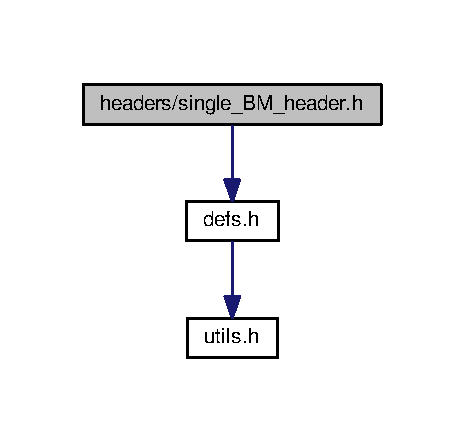
\includegraphics[width=223pt]{single__BM__header_8h__incl}
\end{center}
\end{figure}
\subsection*{Functions}
\begin{DoxyCompactItemize}
\item 
\mbox{\Hypertarget{single__BM__header_8h_a581c807c32dcbab09f5a73cd24757fc3}\label{single__BM__header_8h_a581c807c32dcbab09f5a73cd24757fc3}} 
short {\bfseries iso\+Tricode} (\hyperlink{structEDGE__DEVICE}{E\+D\+G\+E\+\_\+\+D\+E\+V\+I\+CE} $\ast$adj\+\_\+list\+\_\+u, \hyperlink{structEDGE__DEVICE}{E\+D\+G\+E\+\_\+\+D\+E\+V\+I\+CE} $\ast$adj\+\_\+list\+\_\+v, \hyperlink{structNODE__DEVICE}{N\+O\+D\+E\+\_\+\+D\+E\+V\+I\+CE} $\ast$u, \hyperlink{structNODE__DEVICE}{N\+O\+D\+E\+\_\+\+D\+E\+V\+I\+CE} $\ast$v, uint w\+\_\+id)
\item 
\mbox{\Hypertarget{single__BM__header_8h_a95f02d51d2e478d2203f203da34ca536}\label{single__BM__header_8h_a95f02d51d2e478d2203f203da34ca536}} 
uint {\bfseries get\+\_\+neighbor\+\_\+id} (\hyperlink{structEDGE__DEVICE}{E\+D\+G\+E\+\_\+\+D\+E\+V\+I\+CE} e)
\item 
\mbox{\Hypertarget{single__BM__header_8h_a3c6ec02b4ab708a4c4cc9d75d8b8bd3d}\label{single__BM__header_8h_a3c6ec02b4ab708a4c4cc9d75d8b8bd3d}} 
\hyperlink{utils_8h_aa268a41a13430b18e933ed40207178d0}{D\+I\+R\+E\+C\+T\+I\+ON} {\bfseries get\+\_\+direction} (\hyperlink{structEDGE__DEVICE}{E\+D\+G\+E\+\_\+\+D\+E\+V\+I\+CE} e)
\item 
\mbox{\Hypertarget{single__BM__header_8h_a1c79c56ad87266e0d11764d24f5983d1}\label{single__BM__header_8h_a1c79c56ad87266e0d11764d24f5983d1}} 
\hyperlink{utils_8h_aa268a41a13430b18e933ed40207178d0}{D\+I\+R\+E\+C\+T\+I\+ON} {\bfseries turnup} (\hyperlink{utils_8h_aa268a41a13430b18e933ed40207178d0}{D\+I\+R\+E\+C\+T\+I\+ON} dir)
\item 
\mbox{\Hypertarget{single__BM__header_8h_adfac5a560df38bc43d0300555971355f}\label{single__BM__header_8h_adfac5a560df38bc43d0300555971355f}} 
int {\bfseries binary\+\_\+search\+\_\+adj\+\_\+list} (\hyperlink{structEDGE__DEVICE}{E\+D\+G\+E\+\_\+\+D\+E\+V\+I\+CE} $\ast$table, uint key, int first, int last)
\item 
\mbox{\Hypertarget{single__BM__header_8h_a92cb3b1f91aa073b09b7c1736c56b52a}\label{single__BM__header_8h_a92cb3b1f91aa073b09b7c1736c56b52a}} 
int {\bfseries linear\+\_\+search\+\_\+adj\+\_\+list} (\hyperlink{structEDGE__DEVICE}{E\+D\+G\+E\+\_\+\+D\+E\+V\+I\+CE} $\ast$table, uint key, uint first, uint last)
\item 
\mbox{\Hypertarget{single__BM__header_8h_a950cef2eb92d33cc0eacbf81043cb8a2}\label{single__BM__header_8h_a950cef2eb92d33cc0eacbf81043cb8a2}} 
uint {\bfseries get\+\_\+node\+\_\+id} (\+\_\+\+\_\+constant \hyperlink{structNODE__DEVICE}{N\+O\+D\+E\+\_\+\+D\+E\+V\+I\+CE} $\ast$n)
\item 
\mbox{\Hypertarget{single__BM__header_8h_a3ff637c927133d471e1ba8915cdb8bf2}\label{single__BM__header_8h_a3ff637c927133d471e1ba8915cdb8bf2}} 
uint {\bfseries get\+\_\+first} (\+\_\+\+\_\+constant \hyperlink{structNODE__DEVICE}{N\+O\+D\+E\+\_\+\+D\+E\+V\+I\+CE} $\ast$n)
\item 
\mbox{\Hypertarget{single__BM__header_8h_ade8df49106a5ef579bf793631c289dd6}\label{single__BM__header_8h_ade8df49106a5ef579bf793631c289dd6}} 
uint {\bfseries get\+\_\+last} (\+\_\+\+\_\+constant \hyperlink{structNODE__DEVICE}{N\+O\+D\+E\+\_\+\+D\+E\+V\+I\+CE} $\ast$n)
\item 
\mbox{\Hypertarget{single__BM__header_8h_a5c89479856a4d5c3a30dcdf6f9111a0c}\label{single__BM__header_8h_a5c89479856a4d5c3a30dcdf6f9111a0c}} 
\hyperlink{structNODE__DEVICE}{N\+O\+D\+E\+\_\+\+D\+E\+V\+I\+CE} {\bfseries copy\+\_\+node} (\+\_\+\+\_\+constant \hyperlink{structNODE__DEVICE}{N\+O\+D\+E\+\_\+\+D\+E\+V\+I\+CE} $\ast$source)
\item 
\mbox{\Hypertarget{single__BM__header_8h_a71a63036deafad558f1e97eab214b229}\label{single__BM__header_8h_a71a63036deafad558f1e97eab214b229}} 
ushort {\bfseries copy\+\_\+edge\+\_\+list} (\+\_\+\+\_\+constant \hyperlink{structEDGE__DEVICE}{E\+D\+G\+E\+\_\+\+D\+E\+V\+I\+CE} $\ast$edges, \hyperlink{structEDGE__DEVICE}{E\+D\+G\+E\+\_\+\+D\+E\+V\+I\+CE} $\ast$local\+\_\+edges, \hyperlink{structNODE__DEVICE}{N\+O\+D\+E\+\_\+\+D\+E\+V\+I\+CE} $\ast$node)
\item 
\mbox{\Hypertarget{single__BM__header_8h_aec484d28063ddf3360c29f3704e6badb}\label{single__BM__header_8h_aec484d28063ddf3360c29f3704e6badb}} 
int {\bfseries get\+\_\+neighbor\+\_\+pos} (\hyperlink{structEDGE__DEVICE}{E\+D\+G\+E\+\_\+\+D\+E\+V\+I\+CE} $\ast$edges, \hyperlink{structNODE__DEVICE}{N\+O\+D\+E\+\_\+\+D\+E\+V\+I\+CE} $\ast$n, uint nid)
\item 
\mbox{\Hypertarget{single__BM__header_8h_a90b9a53d9eaa5596ea7ed1d15683c17a}\label{single__BM__header_8h_a90b9a53d9eaa5596ea7ed1d15683c17a}} 
\hyperlink{utils_8h_aa268a41a13430b18e933ed40207178d0}{D\+I\+R\+E\+C\+T\+I\+ON} {\bfseries get\+\_\+dir\+\_\+between\+\_\+nodes} (\hyperlink{structEDGE__DEVICE}{E\+D\+G\+E\+\_\+\+D\+E\+V\+I\+CE} $\ast$edges, \hyperlink{structNODE__DEVICE}{N\+O\+D\+E\+\_\+\+D\+E\+V\+I\+CE} $\ast$u, uint v\+\_\+id)
\item 
\mbox{\Hypertarget{single__BM__header_8h_a55eff2ab3a319ac3693d954007aca947}\label{single__BM__header_8h_a55eff2ab3a319ac3693d954007aca947}} 
uint {\bfseries get\+\_\+node\+\_\+pos} (\+\_\+\+\_\+constant \hyperlink{structNODE__DEVICE}{N\+O\+D\+E\+\_\+\+D\+E\+V\+I\+CE} $\ast$node\+\_\+list, uint node\+\_\+id, uint num\+\_\+nodes)
\item 
\mbox{\Hypertarget{single__BM__header_8h_a07f4573e769f536ee927d08b1377a0ae}\label{single__BM__header_8h_a07f4573e769f536ee927d08b1377a0ae}} 
int {\bfseries binary\+\_\+search\+\_\+node\+\_\+list\+\_\+norec} (\+\_\+\+\_\+constant \hyperlink{structNODE__DEVICE}{N\+O\+D\+E\+\_\+\+D\+E\+V\+I\+CE} $\ast$table, uint key, uint first, uint last)
\item 
\mbox{\Hypertarget{single__BM__header_8h_a725a5cacdac475b034827d44d37c76f0}\label{single__BM__header_8h_a725a5cacdac475b034827d44d37c76f0}} 
int {\bfseries linear\+\_\+search\+\_\+node\+\_\+list} (\+\_\+\+\_\+constant \hyperlink{structNODE__DEVICE}{N\+O\+D\+E\+\_\+\+D\+E\+V\+I\+CE} $\ast$table, uint key, uint num\+\_\+nodes)
\end{DoxyCompactItemize}


\subsection{Detailed Description}
This file contains the definitions of the functions needed to execute the single BM kernels. 

\begin{DoxyAuthor}{Author}
\+: Carlos Alfaro
\end{DoxyAuthor}
\begin{DoxyDate}{Date}
\+: 17-\/12-\/2017 
\end{DoxyDate}

\hypertarget{triads_8h}{}\section{headers/triads.h File Reference}
\label{triads_8h}\index{headers/triads.\+h@{headers/triads.\+h}}


This file contains the definitions of the functions needed to implement the secuential versions of the Triad Census algorithms. ~\newline
We have implemented the Brute Force (BF) algorithm and the Batagelj and Mrvar\textquotesingle{}s (BM) algorithm.  


{\ttfamily \#include \char`\"{}graph.\+h\char`\"{}}\newline
Include dependency graph for triads.\+h\+:
\nopagebreak
\begin{figure}[H]
\begin{center}
\leavevmode
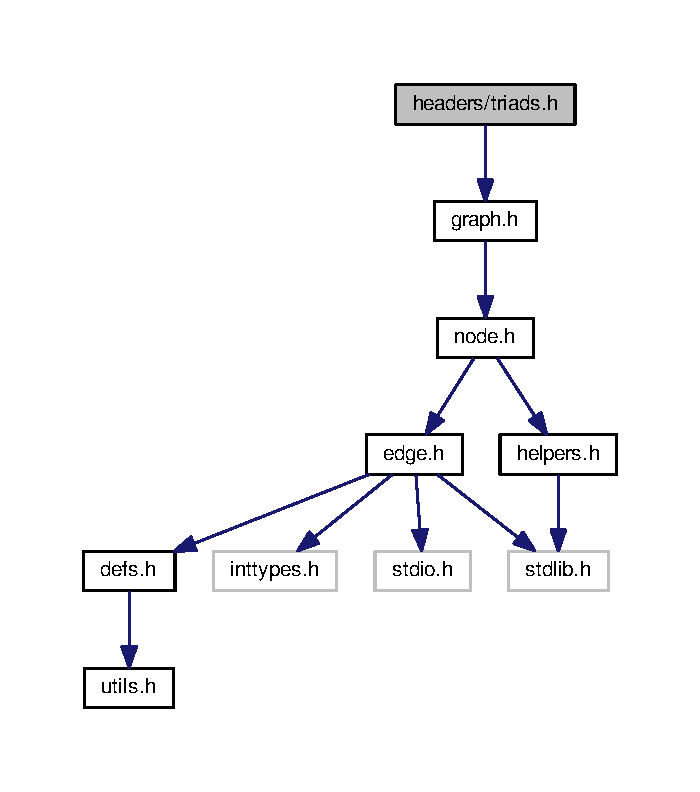
\includegraphics[width=336pt]{triads_8h__incl}
\end{center}
\end{figure}
This graph shows which files directly or indirectly include this file\+:
\nopagebreak
\begin{figure}[H]
\begin{center}
\leavevmode
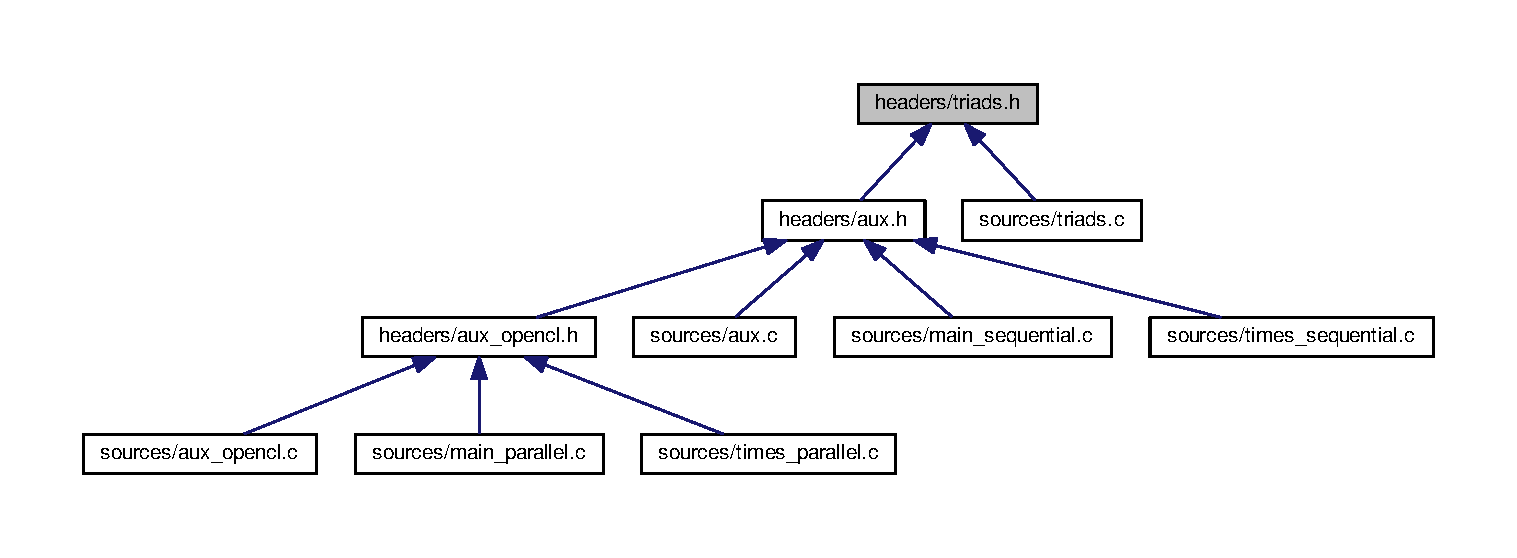
\includegraphics[width=350pt]{triads_8h__dep__incl}
\end{center}
\end{figure}
\subsection*{Functions}
\begin{DoxyCompactItemize}
\item 
uint64\+\_\+t $\ast$ \hyperlink{triads_8h_a33470219fe7e4ce1cf0e82ac26332b54}{triad\+\_\+census\+\_\+\+BF} (\hyperlink{structGRAPH}{G\+R\+A\+PH} $\ast$g)
\begin{DoxyCompactList}\small\item\em Function that implements the Brute Force version of the triad census algorithm. \end{DoxyCompactList}\item 
uint64\+\_\+t $\ast$ \hyperlink{triads_8h_a5a46cb68a0606e745017030524e45098}{triad\+\_\+census\+\_\+\+BM} (\hyperlink{structGRAPH}{G\+R\+A\+PH} $\ast$g)
\begin{DoxyCompactList}\small\item\em Function that implements the Batagelj and Mrvar\textquotesingle{}s version of the triad census algorithm. \end{DoxyCompactList}\item 
void \hyperlink{triads_8h_a1bd1905d86d16197b1549c6d41d53b7f}{print\+\_\+triad\+\_\+census} (uint64\+\_\+t $\ast$triads)
\begin{DoxyCompactList}\small\item\em Function that prints the triad census. \end{DoxyCompactList}\item 
const char $\ast$ \hyperlink{triads_8h_a5b007b930e78fbb00e4febbec02805df}{return\+\_\+code} (int $\ast$census)
\begin{DoxyCompactList}\small\item\em Function returns the code of a triad (for testing purposes) \end{DoxyCompactList}\item 
int \hyperlink{triads_8h_aba89c0fb106399c0731b4cfbcd0e743e}{iso\+Tricode} (\hyperlink{structNODE}{N\+O\+DE} $\ast$u, \hyperlink{structNODE}{N\+O\+DE} $\ast$v, \hyperlink{structNODE}{N\+O\+DE} $\ast$w)
\begin{DoxyCompactList}\small\item\em Function that computes the triad type of a triple of nodes. \end{DoxyCompactList}\item 
uint64\+\_\+t \hyperlink{triads_8h_af9d36341671cf11b24be96d4d1228181}{num\+\_\+total\+\_\+triads} (uint32\+\_\+t n)
\begin{DoxyCompactList}\small\item\em Function that computes and returns the number of triads present in a graph of n nodes. \end{DoxyCompactList}\end{DoxyCompactItemize}


\subsection{Detailed Description}
This file contains the definitions of the functions needed to implement the secuential versions of the Triad Census algorithms. ~\newline
We have implemented the Brute Force (BF) algorithm and the Batagelj and Mrvar\textquotesingle{}s (BM) algorithm. 

\begin{DoxyAuthor}{Author}
\+: Carlos Alfaro
\end{DoxyAuthor}
\begin{DoxyDate}{Date}
\+: 23-\/10-\/2017 
\end{DoxyDate}


\subsection{Function Documentation}
\mbox{\Hypertarget{triads_8h_aba89c0fb106399c0731b4cfbcd0e743e}\label{triads_8h_aba89c0fb106399c0731b4cfbcd0e743e}} 
\index{triads.\+h@{triads.\+h}!iso\+Tricode@{iso\+Tricode}}
\index{iso\+Tricode@{iso\+Tricode}!triads.\+h@{triads.\+h}}
\subsubsection{\texorpdfstring{iso\+Tricode()}{isoTricode()}}
{\footnotesize\ttfamily int iso\+Tricode (\begin{DoxyParamCaption}\item[{\hyperlink{structNODE}{N\+O\+DE} $\ast$}]{u,  }\item[{\hyperlink{structNODE}{N\+O\+DE} $\ast$}]{v,  }\item[{\hyperlink{structNODE}{N\+O\+DE} $\ast$}]{w }\end{DoxyParamCaption})}



Function that computes the triad type of a triple of nodes. 


\begin{DoxyParams}{Parameters}
{\em N\+O\+D\+E$\ast$} & u\+: First node of the triple \\
\hline
{\em N\+O\+D\+E$\ast$} & v\+: Second node of the triple \\
\hline
{\em N\+O\+D\+E$\ast$} & w\+: Third node of the triple\\
\hline
\end{DoxyParams}
\begin{DoxyReturn}{Returns}
int\+: A number between 0 and 15, depending on the configuration of the triple 
\end{DoxyReturn}
\mbox{\Hypertarget{triads_8h_af9d36341671cf11b24be96d4d1228181}\label{triads_8h_af9d36341671cf11b24be96d4d1228181}} 
\index{triads.\+h@{triads.\+h}!num\+\_\+total\+\_\+triads@{num\+\_\+total\+\_\+triads}}
\index{num\+\_\+total\+\_\+triads@{num\+\_\+total\+\_\+triads}!triads.\+h@{triads.\+h}}
\subsubsection{\texorpdfstring{num\+\_\+total\+\_\+triads()}{num\_total\_triads()}}
{\footnotesize\ttfamily uint64\+\_\+t num\+\_\+total\+\_\+triads (\begin{DoxyParamCaption}\item[{uint32\+\_\+t}]{n }\end{DoxyParamCaption})}



Function that computes and returns the number of triads present in a graph of n nodes. 


\begin{DoxyParams}{Parameters}
{\em uint32\+\_\+t} & n\+: The number of nodes of a graph\\
\hline
\end{DoxyParams}
\begin{DoxyReturn}{Returns}
uint32\+\_\+t\+: The number of total triads 
\end{DoxyReturn}
\mbox{\Hypertarget{triads_8h_a1bd1905d86d16197b1549c6d41d53b7f}\label{triads_8h_a1bd1905d86d16197b1549c6d41d53b7f}} 
\index{triads.\+h@{triads.\+h}!print\+\_\+triad\+\_\+census@{print\+\_\+triad\+\_\+census}}
\index{print\+\_\+triad\+\_\+census@{print\+\_\+triad\+\_\+census}!triads.\+h@{triads.\+h}}
\subsubsection{\texorpdfstring{print\+\_\+triad\+\_\+census()}{print\_triad\_census()}}
{\footnotesize\ttfamily void print\+\_\+triad\+\_\+census (\begin{DoxyParamCaption}\item[{uint64\+\_\+t $\ast$}]{triads }\end{DoxyParamCaption})}



Function that prints the triad census. 


\begin{DoxyParams}{Parameters}
{\em int$\ast$} & census\+: The vector containing the triad census\\
\hline
\end{DoxyParams}
\begin{DoxyReturn}{Returns}
None 
\end{DoxyReturn}
\mbox{\Hypertarget{triads_8h_a5b007b930e78fbb00e4febbec02805df}\label{triads_8h_a5b007b930e78fbb00e4febbec02805df}} 
\index{triads.\+h@{triads.\+h}!return\+\_\+code@{return\+\_\+code}}
\index{return\+\_\+code@{return\+\_\+code}!triads.\+h@{triads.\+h}}
\subsubsection{\texorpdfstring{return\+\_\+code()}{return\_code()}}
{\footnotesize\ttfamily const char$\ast$ return\+\_\+code (\begin{DoxyParamCaption}\item[{int $\ast$}]{census }\end{DoxyParamCaption})}



Function returns the code of a triad (for testing purposes) 


\begin{DoxyParams}{Parameters}
{\em int$\ast$} & census\+: The vector containing the triad census\\
\hline
\end{DoxyParams}
\begin{DoxyReturn}{Returns}
const char$\ast$\+: The triad code 
\end{DoxyReturn}
\mbox{\Hypertarget{triads_8h_a33470219fe7e4ce1cf0e82ac26332b54}\label{triads_8h_a33470219fe7e4ce1cf0e82ac26332b54}} 
\index{triads.\+h@{triads.\+h}!triad\+\_\+census\+\_\+\+BF@{triad\+\_\+census\+\_\+\+BF}}
\index{triad\+\_\+census\+\_\+\+BF@{triad\+\_\+census\+\_\+\+BF}!triads.\+h@{triads.\+h}}
\subsubsection{\texorpdfstring{triad\+\_\+census\+\_\+\+B\+F()}{triad\_census\_BF()}}
{\footnotesize\ttfamily uint64\+\_\+t$\ast$ triad\+\_\+census\+\_\+\+BF (\begin{DoxyParamCaption}\item[{\hyperlink{structGRAPH}{G\+R\+A\+PH} $\ast$}]{g }\end{DoxyParamCaption})}



Function that implements the Brute Force version of the triad census algorithm. 


\begin{DoxyParams}{Parameters}
{\em G\+R\+A\+P\+H$\ast$} & g\+: Pointer to the graph of which we want to perform the triad census\\
\hline
\end{DoxyParams}
\begin{DoxyReturn}{Returns}
int$\ast$\+: a vector containing the triad counts 
\end{DoxyReturn}
\mbox{\Hypertarget{triads_8h_a5a46cb68a0606e745017030524e45098}\label{triads_8h_a5a46cb68a0606e745017030524e45098}} 
\index{triads.\+h@{triads.\+h}!triad\+\_\+census\+\_\+\+BM@{triad\+\_\+census\+\_\+\+BM}}
\index{triad\+\_\+census\+\_\+\+BM@{triad\+\_\+census\+\_\+\+BM}!triads.\+h@{triads.\+h}}
\subsubsection{\texorpdfstring{triad\+\_\+census\+\_\+\+B\+M()}{triad\_census\_BM()}}
{\footnotesize\ttfamily uint64\+\_\+t$\ast$ triad\+\_\+census\+\_\+\+BM (\begin{DoxyParamCaption}\item[{\hyperlink{structGRAPH}{G\+R\+A\+PH} $\ast$}]{g }\end{DoxyParamCaption})}



Function that implements the Batagelj and Mrvar\textquotesingle{}s version of the triad census algorithm. 


\begin{DoxyParams}{Parameters}
{\em G\+R\+A\+P\+H$\ast$} & g\+: Pointer to the graph of which we want to perform the triad census\\
\hline
\end{DoxyParams}
\begin{DoxyReturn}{Returns}
int$\ast$\+: a vector containing the triad counts 
\end{DoxyReturn}

\hypertarget{utils_8h}{}\section{headers/utils.h File Reference}
\label{utils_8h}\index{headers/utils.\+h@{headers/utils.\+h}}


This file contains the enumerations and macros needed for the whole project.  


This graph shows which files directly or indirectly include this file\+:
\nopagebreak
\begin{figure}[H]
\begin{center}
\leavevmode
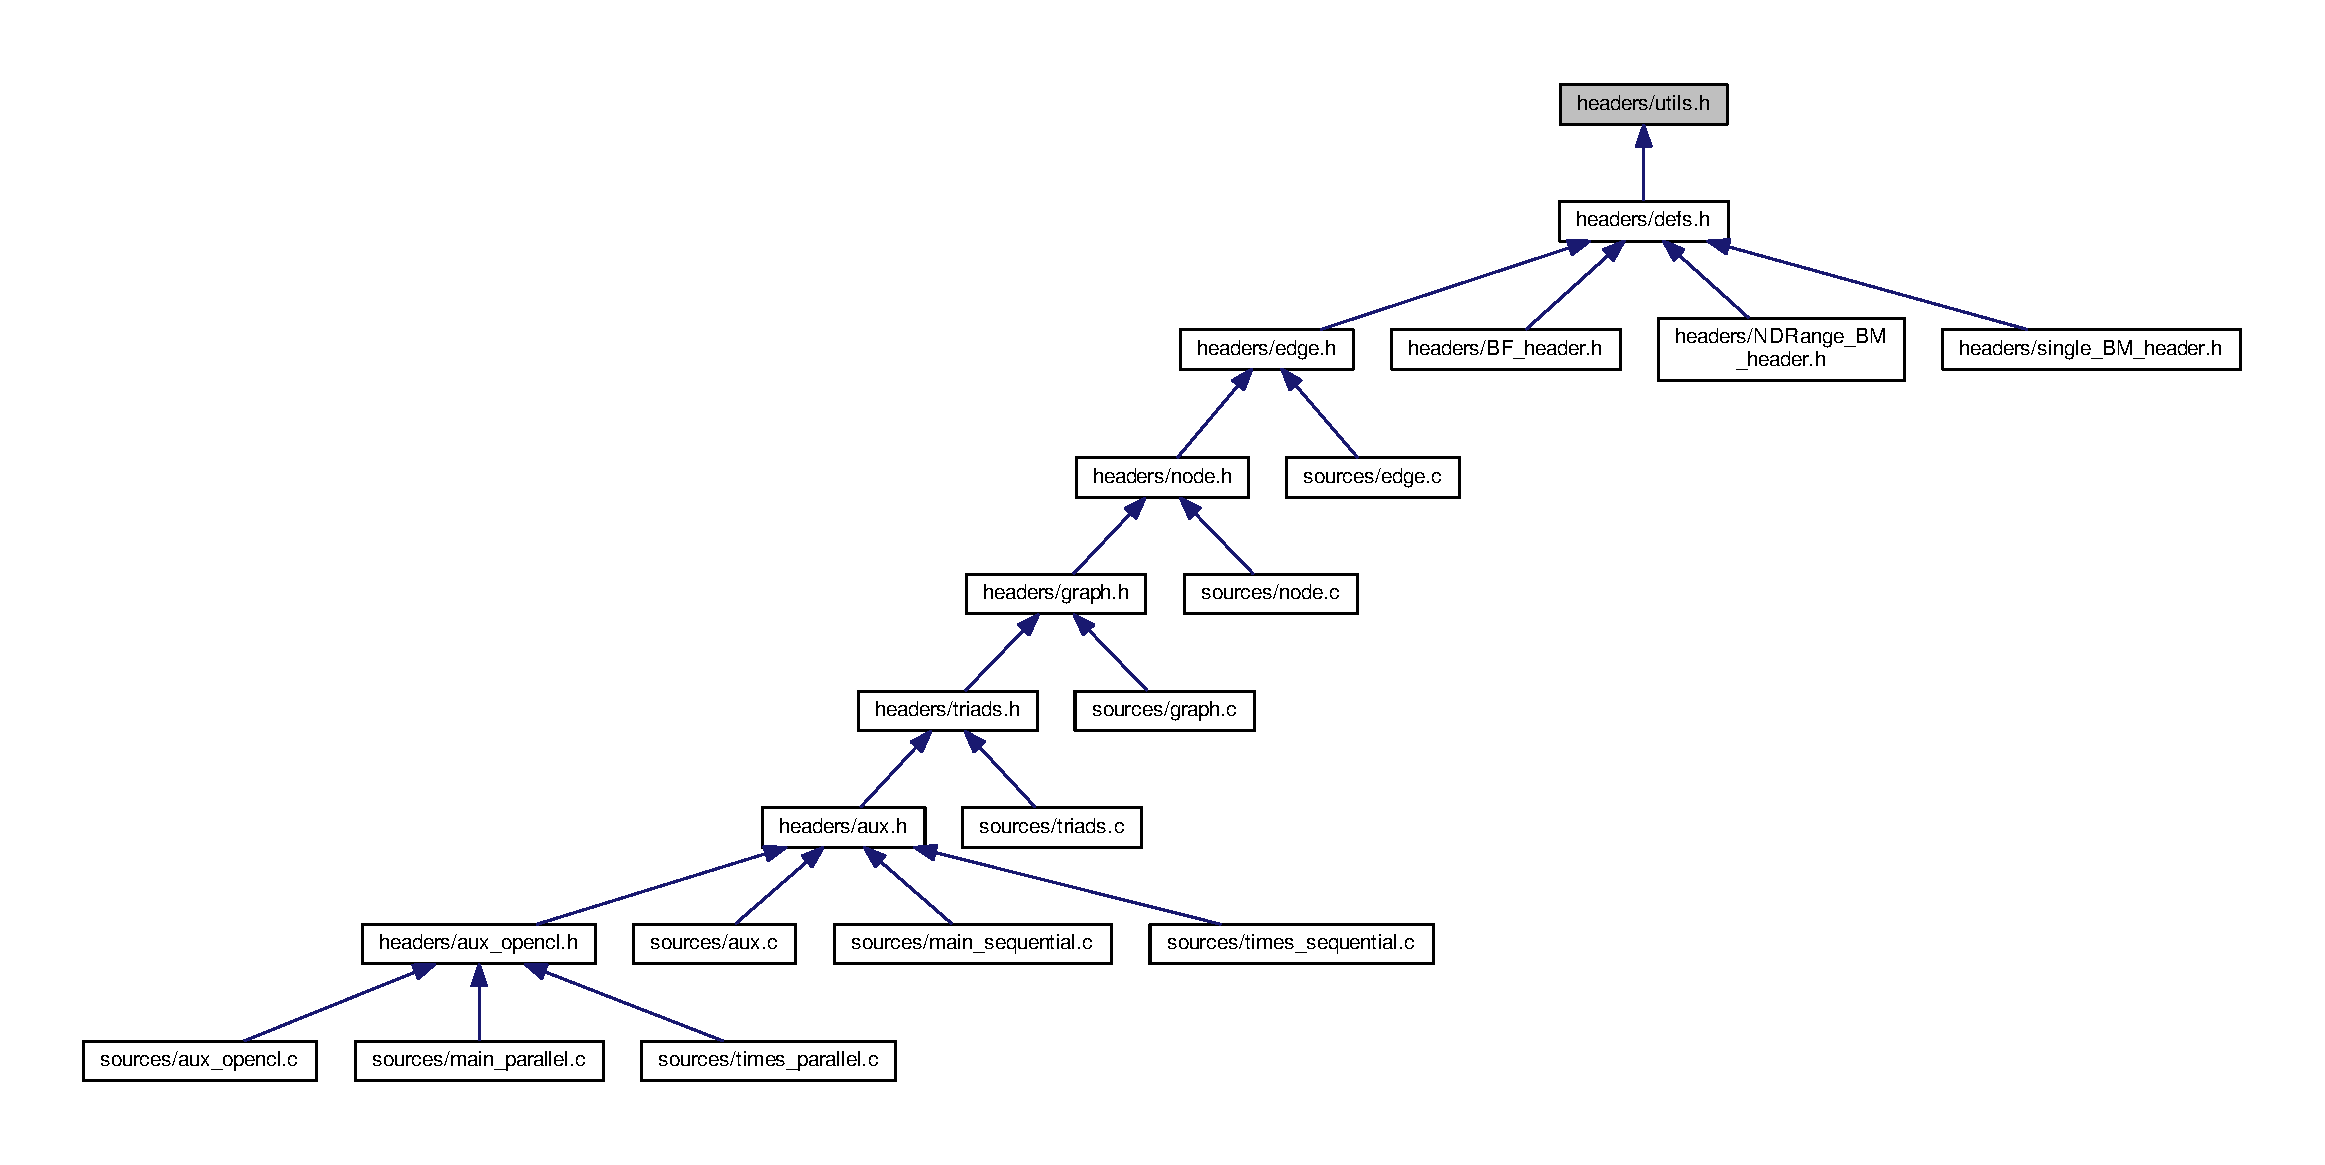
\includegraphics[width=350pt]{utils_8h__dep__incl}
\end{center}
\end{figure}
\subsection*{Macros}
\begin{DoxyCompactItemize}
\item 
\#define \hyperlink{utils_8h_a2b1d39159e4114f433745f15a201c93c}{M\+A\+X\+\_\+\+N\+E\+I\+G\+H\+B\+O\+RS}~100000
\item 
\#define \hyperlink{utils_8h_ab2bde72626290c6daf5da1e9517aa8fb}{N\+U\+M\+\_\+\+T\+R\+I\+A\+DS}~16
\end{DoxyCompactItemize}
\subsection*{Enumerations}
\begin{DoxyCompactItemize}
\item 
enum \hyperlink{utils_8h_a3e5b8192e7d9ffaf3542f1210aec18dd}{B\+O\+OL} \{ \hyperlink{utils_8h_a3e5b8192e7d9ffaf3542f1210aec18ddaa1e095cc966dbecf6a0d8aad75348d1a}{F\+A\+L\+SE} = 0, 
\hyperlink{utils_8h_a3e5b8192e7d9ffaf3542f1210aec18ddaa82764c3079aea4e60c80e45befbb839}{T\+R\+UE}
 \}
\item 
enum \hyperlink{utils_8h_a32c27cc471df37f4fc818d65de0a56c4}{S\+T\+A\+T\+US} \{ \hyperlink{utils_8h_a32c27cc471df37f4fc818d65de0a56c4a0f886785b600b91048fcdc434c6b4a8e}{E\+RR} =-\/1, 
\hyperlink{utils_8h_a32c27cc471df37f4fc818d65de0a56c4a2bc49ec37d6a5715dd23e85f1ff5bb59}{OK}
 \}
\item 
enum \hyperlink{utils_8h_aa268a41a13430b18e933ed40207178d0}{D\+I\+R\+E\+C\+T\+I\+ON} \{ \hyperlink{utils_8h_aa268a41a13430b18e933ed40207178d0ac157bdf0b85a40d2619cbc8bc1ae5fe2}{N\+O\+NE} = 0, 
\hyperlink{utils_8h_aa268a41a13430b18e933ed40207178d0a3cb71bef2a565b674969c7ee4aa7340c}{I\+N\+\_\+\+O\+UT}, 
\hyperlink{utils_8h_aa268a41a13430b18e933ed40207178d0ab5dfd9a720b522f958322f0a6f2215ed}{O\+U\+T\+\_\+\+IN}, 
\hyperlink{utils_8h_aa268a41a13430b18e933ed40207178d0ad136b9b8eb37198a3ce7e36b925dacd7}{B\+I\+D\+I\+R\+E\+C\+T\+I\+O\+N\+AL}
 \}
\end{DoxyCompactItemize}


\subsection{Detailed Description}
This file contains the enumerations and macros needed for the whole project. 

\begin{DoxyAuthor}{Author}
\+: Carlos Alfaro
\end{DoxyAuthor}
\begin{DoxyDate}{Date}
\+: 13-\/10-\/2017 
\end{DoxyDate}


\subsection{Macro Definition Documentation}
\mbox{\Hypertarget{utils_8h_a2b1d39159e4114f433745f15a201c93c}\label{utils_8h_a2b1d39159e4114f433745f15a201c93c}} 
\index{utils.\+h@{utils.\+h}!M\+A\+X\+\_\+\+N\+E\+I\+G\+H\+B\+O\+RS@{M\+A\+X\+\_\+\+N\+E\+I\+G\+H\+B\+O\+RS}}
\index{M\+A\+X\+\_\+\+N\+E\+I\+G\+H\+B\+O\+RS@{M\+A\+X\+\_\+\+N\+E\+I\+G\+H\+B\+O\+RS}!utils.\+h@{utils.\+h}}
\subsubsection{\texorpdfstring{M\+A\+X\+\_\+\+N\+E\+I\+G\+H\+B\+O\+RS}{MAX\_NEIGHBORS}}
{\footnotesize\ttfamily \#define M\+A\+X\+\_\+\+N\+E\+I\+G\+H\+B\+O\+RS~100000}

Maximum number of neighbors supported \mbox{\Hypertarget{utils_8h_ab2bde72626290c6daf5da1e9517aa8fb}\label{utils_8h_ab2bde72626290c6daf5da1e9517aa8fb}} 
\index{utils.\+h@{utils.\+h}!N\+U\+M\+\_\+\+T\+R\+I\+A\+DS@{N\+U\+M\+\_\+\+T\+R\+I\+A\+DS}}
\index{N\+U\+M\+\_\+\+T\+R\+I\+A\+DS@{N\+U\+M\+\_\+\+T\+R\+I\+A\+DS}!utils.\+h@{utils.\+h}}
\subsubsection{\texorpdfstring{N\+U\+M\+\_\+\+T\+R\+I\+A\+DS}{NUM\_TRIADS}}
{\footnotesize\ttfamily \#define N\+U\+M\+\_\+\+T\+R\+I\+A\+DS~16}

Number of isomorphic triad classes 

\subsection{Enumeration Type Documentation}
\mbox{\Hypertarget{utils_8h_a3e5b8192e7d9ffaf3542f1210aec18dd}\label{utils_8h_a3e5b8192e7d9ffaf3542f1210aec18dd}} 
\index{utils.\+h@{utils.\+h}!B\+O\+OL@{B\+O\+OL}}
\index{B\+O\+OL@{B\+O\+OL}!utils.\+h@{utils.\+h}}
\subsubsection{\texorpdfstring{B\+O\+OL}{BOOL}}
{\footnotesize\ttfamily enum \hyperlink{utils_8h_a3e5b8192e7d9ffaf3542f1210aec18dd}{B\+O\+OL}}

\begin{DoxyEnumFields}{Enumerator}
\raisebox{\heightof{T}}[0pt][0pt]{\index{F\+A\+L\+SE@{F\+A\+L\+SE}!utils.\+h@{utils.\+h}}\index{utils.\+h@{utils.\+h}!F\+A\+L\+SE@{F\+A\+L\+SE}}}\mbox{\Hypertarget{utils_8h_a3e5b8192e7d9ffaf3542f1210aec18ddaa1e095cc966dbecf6a0d8aad75348d1a}\label{utils_8h_a3e5b8192e7d9ffaf3542f1210aec18ddaa1e095cc966dbecf6a0d8aad75348d1a}} 
F\+A\+L\+SE&Boolean value F\+A\+L\+SE \\
\hline

\raisebox{\heightof{T}}[0pt][0pt]{\index{T\+R\+UE@{T\+R\+UE}!utils.\+h@{utils.\+h}}\index{utils.\+h@{utils.\+h}!T\+R\+UE@{T\+R\+UE}}}\mbox{\Hypertarget{utils_8h_a3e5b8192e7d9ffaf3542f1210aec18ddaa82764c3079aea4e60c80e45befbb839}\label{utils_8h_a3e5b8192e7d9ffaf3542f1210aec18ddaa82764c3079aea4e60c80e45befbb839}} 
T\+R\+UE&Boolean value F\+A\+L\+SE \\
\hline

\end{DoxyEnumFields}
\mbox{\Hypertarget{utils_8h_aa268a41a13430b18e933ed40207178d0}\label{utils_8h_aa268a41a13430b18e933ed40207178d0}} 
\index{utils.\+h@{utils.\+h}!D\+I\+R\+E\+C\+T\+I\+ON@{D\+I\+R\+E\+C\+T\+I\+ON}}
\index{D\+I\+R\+E\+C\+T\+I\+ON@{D\+I\+R\+E\+C\+T\+I\+ON}!utils.\+h@{utils.\+h}}
\subsubsection{\texorpdfstring{D\+I\+R\+E\+C\+T\+I\+ON}{DIRECTION}}
{\footnotesize\ttfamily enum \hyperlink{utils_8h_aa268a41a13430b18e933ed40207178d0}{D\+I\+R\+E\+C\+T\+I\+ON}}

Status enumeration (for return values) \begin{DoxyEnumFields}{Enumerator}
\raisebox{\heightof{T}}[0pt][0pt]{\index{N\+O\+NE@{N\+O\+NE}!utils.\+h@{utils.\+h}}\index{utils.\+h@{utils.\+h}!N\+O\+NE@{N\+O\+NE}}}\mbox{\Hypertarget{utils_8h_aa268a41a13430b18e933ed40207178d0ac157bdf0b85a40d2619cbc8bc1ae5fe2}\label{utils_8h_aa268a41a13430b18e933ed40207178d0ac157bdf0b85a40d2619cbc8bc1ae5fe2}} 
N\+O\+NE&No edge \\
\hline

\raisebox{\heightof{T}}[0pt][0pt]{\index{I\+N\+\_\+\+O\+UT@{I\+N\+\_\+\+O\+UT}!utils.\+h@{utils.\+h}}\index{utils.\+h@{utils.\+h}!I\+N\+\_\+\+O\+UT@{I\+N\+\_\+\+O\+UT}}}\mbox{\Hypertarget{utils_8h_aa268a41a13430b18e933ed40207178d0a3cb71bef2a565b674969c7ee4aa7340c}\label{utils_8h_aa268a41a13430b18e933ed40207178d0a3cb71bef2a565b674969c7ee4aa7340c}} 
I\+N\+\_\+\+O\+UT&Outgoing edge \\
\hline

\raisebox{\heightof{T}}[0pt][0pt]{\index{O\+U\+T\+\_\+\+IN@{O\+U\+T\+\_\+\+IN}!utils.\+h@{utils.\+h}}\index{utils.\+h@{utils.\+h}!O\+U\+T\+\_\+\+IN@{O\+U\+T\+\_\+\+IN}}}\mbox{\Hypertarget{utils_8h_aa268a41a13430b18e933ed40207178d0ab5dfd9a720b522f958322f0a6f2215ed}\label{utils_8h_aa268a41a13430b18e933ed40207178d0ab5dfd9a720b522f958322f0a6f2215ed}} 
O\+U\+T\+\_\+\+IN&Incoming edge \\
\hline

\raisebox{\heightof{T}}[0pt][0pt]{\index{B\+I\+D\+I\+R\+E\+C\+T\+I\+O\+N\+AL@{B\+I\+D\+I\+R\+E\+C\+T\+I\+O\+N\+AL}!utils.\+h@{utils.\+h}}\index{utils.\+h@{utils.\+h}!B\+I\+D\+I\+R\+E\+C\+T\+I\+O\+N\+AL@{B\+I\+D\+I\+R\+E\+C\+T\+I\+O\+N\+AL}}}\mbox{\Hypertarget{utils_8h_aa268a41a13430b18e933ed40207178d0ad136b9b8eb37198a3ce7e36b925dacd7}\label{utils_8h_aa268a41a13430b18e933ed40207178d0ad136b9b8eb37198a3ce7e36b925dacd7}} 
B\+I\+D\+I\+R\+E\+C\+T\+I\+O\+N\+AL&Bidirectional edge \\
\hline

\end{DoxyEnumFields}
\mbox{\Hypertarget{utils_8h_a32c27cc471df37f4fc818d65de0a56c4}\label{utils_8h_a32c27cc471df37f4fc818d65de0a56c4}} 
\index{utils.\+h@{utils.\+h}!S\+T\+A\+T\+US@{S\+T\+A\+T\+US}}
\index{S\+T\+A\+T\+US@{S\+T\+A\+T\+US}!utils.\+h@{utils.\+h}}
\subsubsection{\texorpdfstring{S\+T\+A\+T\+US}{STATUS}}
{\footnotesize\ttfamily enum \hyperlink{utils_8h_a32c27cc471df37f4fc818d65de0a56c4}{S\+T\+A\+T\+US}}

Boolean enumeration \begin{DoxyEnumFields}{Enumerator}
\raisebox{\heightof{T}}[0pt][0pt]{\index{E\+RR@{E\+RR}!utils.\+h@{utils.\+h}}\index{utils.\+h@{utils.\+h}!E\+RR@{E\+RR}}}\mbox{\Hypertarget{utils_8h_a32c27cc471df37f4fc818d65de0a56c4a0f886785b600b91048fcdc434c6b4a8e}\label{utils_8h_a32c27cc471df37f4fc818d65de0a56c4a0f886785b600b91048fcdc434c6b4a8e}} 
E\+RR&Error \\
\hline

\raisebox{\heightof{T}}[0pt][0pt]{\index{OK@{OK}!utils.\+h@{utils.\+h}}\index{utils.\+h@{utils.\+h}!OK@{OK}}}\mbox{\Hypertarget{utils_8h_a32c27cc471df37f4fc818d65de0a56c4a2bc49ec37d6a5715dd23e85f1ff5bb59}\label{utils_8h_a32c27cc471df37f4fc818d65de0a56c4a2bc49ec37d6a5715dd23e85f1ff5bb59}} 
OK&Successful execution \\
\hline

\end{DoxyEnumFields}

\hypertarget{aux_8c}{}\section{sources/aux.c File Reference}
\label{aux_8c}\index{sources/aux.\+c@{sources/aux.\+c}}


This file contains the code that implements the functions defined in the header file \hyperlink{aux_8h}{aux.\+h}. Please refer to it to check the documentation.  


{\ttfamily \#include \char`\"{}../headers/aux.\+h\char`\"{}}\newline
Include dependency graph for aux.\+c\+:
\nopagebreak
\begin{figure}[H]
\begin{center}
\leavevmode
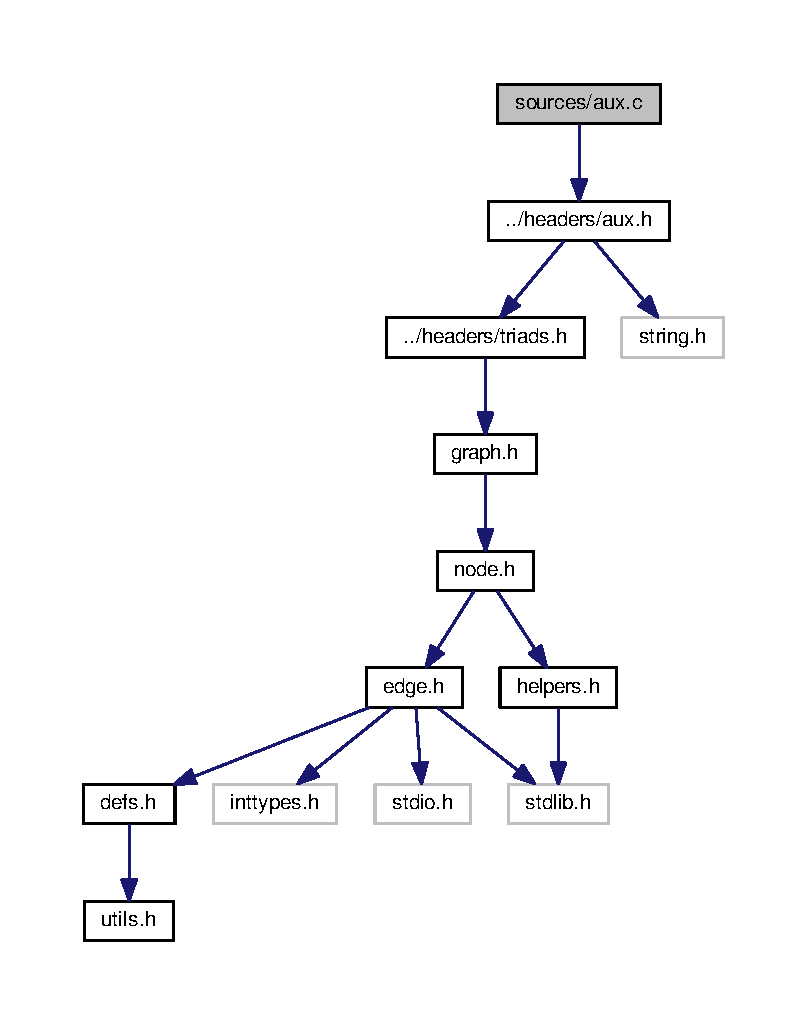
\includegraphics[width=350pt]{aux_8c__incl}
\end{center}
\end{figure}
\subsection*{Functions}
\begin{DoxyCompactItemize}
\item 
void \hyperlink{aux_8c_a2d7f0126a191ecc47001de15e44eb4f9}{display\+\_\+graph\+\_\+summary} (\hyperlink{structGRAPH}{G\+R\+A\+PH} $\ast$g)
\begin{DoxyCompactList}\small\item\em Function that displays a summary of graph g printing its number of nodes, edges and triads. \end{DoxyCompactList}\item 
\hyperlink{utils_8h_a3e5b8192e7d9ffaf3542f1210aec18dd}{B\+O\+OL} \hyperlink{aux_8c_a2f5ae95e590fba7aaae015b750080579}{is\+\_\+ordered\+\_\+kernel} (char $\ast$name\+\_\+kernel)
\begin{DoxyCompactList}\small\item\em Function that checks the name of a kernel to discover if the kernel expects ordered input. \end{DoxyCompactList}\item 
\hyperlink{utils_8h_a3e5b8192e7d9ffaf3542f1210aec18dd}{B\+O\+OL} \hyperlink{aux_8c_abe467f2222de7b22db9f67f5ce6a529c}{is\+\_\+\+N\+D\+Range\+\_\+kernel} (char $\ast$name\+\_\+kernel)
\begin{DoxyCompactList}\small\item\em Function that checks the name of a kernel to discover if the kernel is a N\+D\+Range kernel. \end{DoxyCompactList}\item 
\hyperlink{utils_8h_a3e5b8192e7d9ffaf3542f1210aec18dd}{B\+O\+OL} \hyperlink{aux_8c_a1b1e4c6a6f5d3a0fc38e4c4cd17aa8e5}{is\+\_\+\+B\+M\+\_\+kernel} (char $\ast$name\+\_\+kernel)
\begin{DoxyCompactList}\small\item\em Function that checks the name of a kernel to discover if the kernel implements a BM algorithm. \end{DoxyCompactList}\item 
void \hyperlink{aux_8c_afc44cd39add4462b508953982dfa66b7}{write\+\_\+times} (char $\ast$times\+\_\+name, \hyperlink{structGRAPH}{G\+R\+A\+PH} $\ast$g, double reading\+\_\+time, double execution\+\_\+time)
\begin{DoxyCompactList}\small\item\em Function that writes performance data to a file. \end{DoxyCompactList}\item 
void \hyperlink{aux_8c_a3f18520902448cec9b1693f8914ca023}{rand\+\_\+graph\+\_\+generation} (unsigned int num\+\_\+nodes, unsigned int num\+\_\+edges, unsigned int seed, char $\ast$namefile)
\begin{DoxyCompactList}\small\item\em Function that randomly generates a graph and writes it to a file. \end{DoxyCompactList}\end{DoxyCompactItemize}


\subsection{Detailed Description}
This file contains the code that implements the functions defined in the header file \hyperlink{aux_8h}{aux.\+h}. Please refer to it to check the documentation. 

\begin{DoxyAuthor}{Author}
\+: Carlos Alfaro
\end{DoxyAuthor}
\begin{DoxyDate}{Date}
\+: 18-\/12-\/2017 
\end{DoxyDate}


\subsection{Function Documentation}
\mbox{\Hypertarget{aux_8c_a2d7f0126a191ecc47001de15e44eb4f9}\label{aux_8c_a2d7f0126a191ecc47001de15e44eb4f9}} 
\index{aux.\+c@{aux.\+c}!display\+\_\+graph\+\_\+summary@{display\+\_\+graph\+\_\+summary}}
\index{display\+\_\+graph\+\_\+summary@{display\+\_\+graph\+\_\+summary}!aux.\+c@{aux.\+c}}
\subsubsection{\texorpdfstring{display\+\_\+graph\+\_\+summary()}{display\_graph\_summary()}}
{\footnotesize\ttfamily void display\+\_\+graph\+\_\+summary (\begin{DoxyParamCaption}\item[{\hyperlink{structGRAPH}{G\+R\+A\+PH} $\ast$}]{g }\end{DoxyParamCaption})}



Function that displays a summary of graph g printing its number of nodes, edges and triads. 


\begin{DoxyParams}{Parameters}
{\em G\+R\+A\+P\+H$\ast$} & g\+: The input graph.\\
\hline
\end{DoxyParams}
\begin{DoxyReturn}{Returns}
None 
\end{DoxyReturn}
\mbox{\Hypertarget{aux_8c_a1b1e4c6a6f5d3a0fc38e4c4cd17aa8e5}\label{aux_8c_a1b1e4c6a6f5d3a0fc38e4c4cd17aa8e5}} 
\index{aux.\+c@{aux.\+c}!is\+\_\+\+B\+M\+\_\+kernel@{is\+\_\+\+B\+M\+\_\+kernel}}
\index{is\+\_\+\+B\+M\+\_\+kernel@{is\+\_\+\+B\+M\+\_\+kernel}!aux.\+c@{aux.\+c}}
\subsubsection{\texorpdfstring{is\+\_\+\+B\+M\+\_\+kernel()}{is\_BM\_kernel()}}
{\footnotesize\ttfamily \hyperlink{utils_8h_a3e5b8192e7d9ffaf3542f1210aec18dd}{B\+O\+OL} is\+\_\+\+B\+M\+\_\+kernel (\begin{DoxyParamCaption}\item[{char $\ast$}]{name\+\_\+kernel }\end{DoxyParamCaption})}



Function that checks the name of a kernel to discover if the kernel implements a BM algorithm. 


\begin{DoxyParams}{Parameters}
{\em char$\ast$} & name\+\_\+kernel\+: The name of the kernel.\\
\hline
\end{DoxyParams}
\begin{DoxyReturn}{Returns}
B\+O\+OL\+: T\+R\+UE if the kernel implements BM.~\newline
 F\+A\+L\+SE otherwise 
\end{DoxyReturn}
\mbox{\Hypertarget{aux_8c_abe467f2222de7b22db9f67f5ce6a529c}\label{aux_8c_abe467f2222de7b22db9f67f5ce6a529c}} 
\index{aux.\+c@{aux.\+c}!is\+\_\+\+N\+D\+Range\+\_\+kernel@{is\+\_\+\+N\+D\+Range\+\_\+kernel}}
\index{is\+\_\+\+N\+D\+Range\+\_\+kernel@{is\+\_\+\+N\+D\+Range\+\_\+kernel}!aux.\+c@{aux.\+c}}
\subsubsection{\texorpdfstring{is\+\_\+\+N\+D\+Range\+\_\+kernel()}{is\_NDRange\_kernel()}}
{\footnotesize\ttfamily \hyperlink{utils_8h_a3e5b8192e7d9ffaf3542f1210aec18dd}{B\+O\+OL} is\+\_\+\+N\+D\+Range\+\_\+kernel (\begin{DoxyParamCaption}\item[{char $\ast$}]{name\+\_\+kernel }\end{DoxyParamCaption})}



Function that checks the name of a kernel to discover if the kernel is a N\+D\+Range kernel. 


\begin{DoxyParams}{Parameters}
{\em char$\ast$} & name\+\_\+kernel\+: The name of the kernel.\\
\hline
\end{DoxyParams}
\begin{DoxyReturn}{Returns}
B\+O\+OL\+: T\+R\+UE if it is a N\+D\+Range kernel.~\newline
 F\+A\+L\+SE otherwise 
\end{DoxyReturn}
\mbox{\Hypertarget{aux_8c_a2f5ae95e590fba7aaae015b750080579}\label{aux_8c_a2f5ae95e590fba7aaae015b750080579}} 
\index{aux.\+c@{aux.\+c}!is\+\_\+ordered\+\_\+kernel@{is\+\_\+ordered\+\_\+kernel}}
\index{is\+\_\+ordered\+\_\+kernel@{is\+\_\+ordered\+\_\+kernel}!aux.\+c@{aux.\+c}}
\subsubsection{\texorpdfstring{is\+\_\+ordered\+\_\+kernel()}{is\_ordered\_kernel()}}
{\footnotesize\ttfamily \hyperlink{utils_8h_a3e5b8192e7d9ffaf3542f1210aec18dd}{B\+O\+OL} is\+\_\+ordered\+\_\+kernel (\begin{DoxyParamCaption}\item[{char $\ast$}]{name\+\_\+kernel }\end{DoxyParamCaption})}



Function that checks the name of a kernel to discover if the kernel expects ordered input. 


\begin{DoxyParams}{Parameters}
{\em char$\ast$} & name\+\_\+kernel\+: The name of the kernel.\\
\hline
\end{DoxyParams}
\begin{DoxyReturn}{Returns}
B\+O\+OL\+: T\+R\+UE if the kernel expects ordered input.~\newline
 F\+A\+L\+SE otherwise 
\end{DoxyReturn}
\mbox{\Hypertarget{aux_8c_a3f18520902448cec9b1693f8914ca023}\label{aux_8c_a3f18520902448cec9b1693f8914ca023}} 
\index{aux.\+c@{aux.\+c}!rand\+\_\+graph\+\_\+generation@{rand\+\_\+graph\+\_\+generation}}
\index{rand\+\_\+graph\+\_\+generation@{rand\+\_\+graph\+\_\+generation}!aux.\+c@{aux.\+c}}
\subsubsection{\texorpdfstring{rand\+\_\+graph\+\_\+generation()}{rand\_graph\_generation()}}
{\footnotesize\ttfamily void rand\+\_\+graph\+\_\+generation (\begin{DoxyParamCaption}\item[{unsigned int}]{num\+\_\+nodes,  }\item[{unsigned int}]{num\+\_\+edges,  }\item[{unsigned int}]{seed,  }\item[{char $\ast$}]{namefile }\end{DoxyParamCaption})}



Function that randomly generates a graph and writes it to a file. 


\begin{DoxyParams}{Parameters}
{\em unsigned} & int num\+\_\+nodes\+: Number of nodes desired. \\
\hline
{\em unsigned} & int num\+\_\+edges\+: Number of edges desired. \\
\hline
{\em unsigned} & int seed\+: The seed for rand() function \\
\hline
{\em char$\ast$} & namefile\+: The name of the file in which to write the graph.\\
\hline
\end{DoxyParams}
\begin{DoxyReturn}{Returns}
None 
\end{DoxyReturn}
\mbox{\Hypertarget{aux_8c_afc44cd39add4462b508953982dfa66b7}\label{aux_8c_afc44cd39add4462b508953982dfa66b7}} 
\index{aux.\+c@{aux.\+c}!write\+\_\+times@{write\+\_\+times}}
\index{write\+\_\+times@{write\+\_\+times}!aux.\+c@{aux.\+c}}
\subsubsection{\texorpdfstring{write\+\_\+times()}{write\_times()}}
{\footnotesize\ttfamily void write\+\_\+times (\begin{DoxyParamCaption}\item[{char $\ast$}]{times\+\_\+name,  }\item[{\hyperlink{structGRAPH}{G\+R\+A\+PH} $\ast$}]{g,  }\item[{double}]{reading\+\_\+time,  }\item[{double}]{execution\+\_\+time }\end{DoxyParamCaption})}



Function that writes performance data to a file. 


\begin{DoxyParams}{Parameters}
{\em char$\ast$} & times\+\_\+name\+: The name of the file in which to write the results. \\
\hline
{\em G\+R\+A\+P\+H$\ast$} & g\+: The graph under analysis. \\
\hline
{\em double} & reading\+\_\+time\+: Graph reading time. \\
\hline
{\em double} & execution time\+: Triad census execution time.\\
\hline
\end{DoxyParams}
\begin{DoxyReturn}{Returns}
None 
\end{DoxyReturn}

\hypertarget{aux__opencl_8c}{}\section{sources/aux\+\_\+opencl.c File Reference}
\label{aux__opencl_8c}\index{sources/aux\+\_\+opencl.\+c@{sources/aux\+\_\+opencl.\+c}}


This file contains the code that implements the functions defined in the header file \hyperlink{aux__opencl_8h}{aux\+\_\+opencl.\+h}. Please refer to it to check the documentation.  


{\ttfamily \#include \char`\"{}../headers/aux\+\_\+opencl.\+h\char`\"{}}\newline
Include dependency graph for aux\+\_\+opencl.\+c\+:
\nopagebreak
\begin{figure}[H]
\begin{center}
\leavevmode
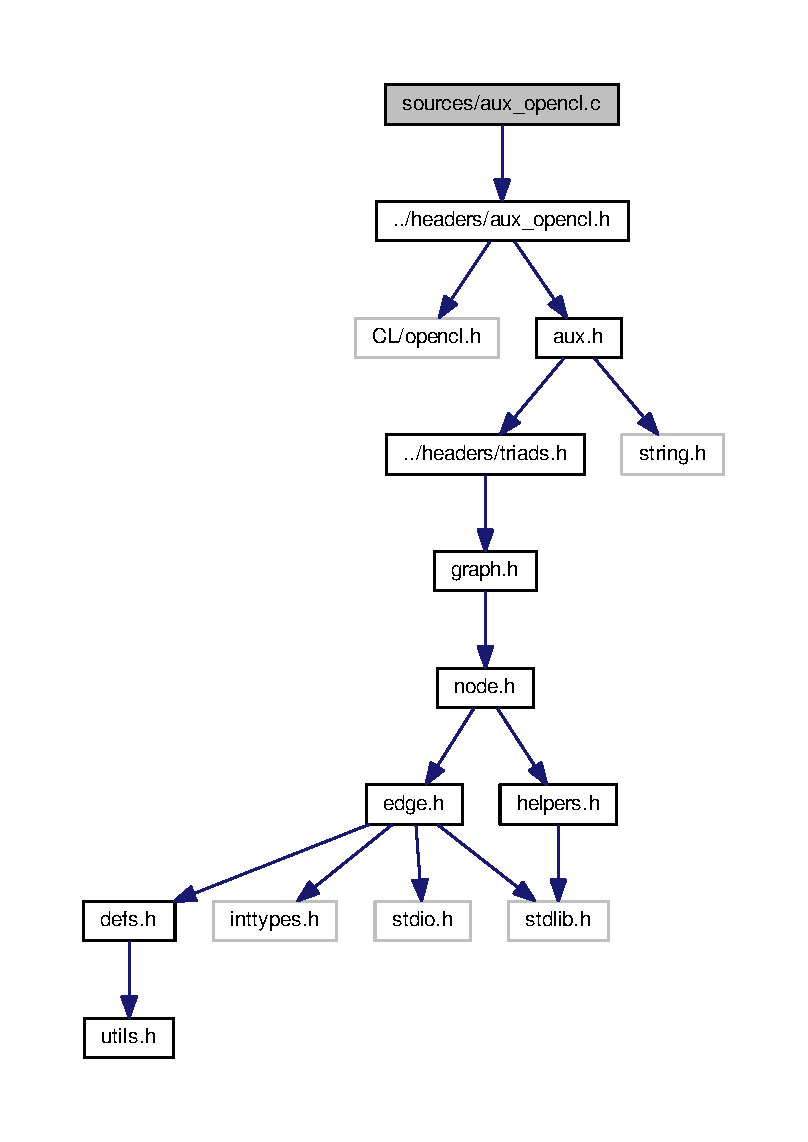
\includegraphics[width=350pt]{aux__opencl_8c__incl}
\end{center}
\end{figure}
\subsection*{Functions}
\begin{DoxyCompactItemize}
\item 
void \hyperlink{aux__opencl_8c_ae9b40ed1990a1e4162a6b6c4fe8419a5}{setup} (cl\+\_\+platform\+\_\+id $\ast$platform, cl\+\_\+device\+\_\+id $\ast$device, cl\+\_\+context $\ast$context)
\begin{DoxyCompactList}\small\item\em Function sets up the proper Open\+CL environment for creating and executing kernels.~\newline
This process involves selecting an Open\+CL platform and an attached device, as well as creating an execution context. \end{DoxyCompactList}\item 
cl\+\_\+program \hyperlink{aux__opencl_8c_a335b0aeeb63d503ee152a3adc84ab19e}{create\+\_\+build\+\_\+program} (char $\ast$filename, cl\+\_\+context context, cl\+\_\+device\+\_\+id $\ast$device)
\begin{DoxyCompactList}\small\item\em Function creates and builds the program from a binary .aocx file~\newline
This process involves selecting an Open\+CL platform and an attached device, as well as creating an execution context. \end{DoxyCompactList}\item 
void \hyperlink{aux__opencl_8c_a8e2f457f73112edd95ab085f5de0d4bd}{display\+\_\+platform\+\_\+info} (cl\+\_\+platform\+\_\+id platform)
\begin{DoxyCompactList}\small\item\em Function displays information about the Open\+CL platform. \end{DoxyCompactList}\item 
void \hyperlink{aux__opencl_8c_ab9ec1cbdd471182d6d645cb348ddcfa0}{display\+\_\+device\+\_\+info} (cl\+\_\+device\+\_\+id device)
\begin{DoxyCompactList}\small\item\em Function displays information about the Open\+CL device used. \end{DoxyCompactList}\item 
void \hyperlink{aux__opencl_8c_a2e23d888af16d40462205572135139a4}{check\+\_\+error} (cl\+\_\+int error\+\_\+code, const char $\ast$message)
\begin{DoxyCompactList}\small\item\em Function checks the error code returned by a A\+PI function. If there has been~\newline
an error, displays the errror code and stops execution. \end{DoxyCompactList}\item 
cl\+\_\+mem \hyperlink{aux__opencl_8c_a611ba60155d74de941fd81b533d28c1a}{create\+\_\+and\+\_\+write\+\_\+buffer} (cl\+\_\+context context, cl\+\_\+command\+\_\+queue queue, size\+\_\+t size, void $\ast$host\+\_\+ptr)
\begin{DoxyCompactList}\small\item\em Function that creates an Open\+CL buffer object and fills it with certain information. \end{DoxyCompactList}\item 
void \hyperlink{aux__opencl_8c_afefd6c0004b4a7972a5f55cb8f386211}{set\+\_\+args} (cl\+\_\+kernel kernel, void $\ast$arg0, void $\ast$arg1, void $\ast$arg2, void $\ast$arg3)
\begin{DoxyCompactList}\small\item\em Function that sets the four argument of an Open\+CL kernel. \end{DoxyCompactList}\end{DoxyCompactItemize}


\subsection{Detailed Description}
This file contains the code that implements the functions defined in the header file \hyperlink{aux__opencl_8h}{aux\+\_\+opencl.\+h}. Please refer to it to check the documentation. 

\begin{DoxyAuthor}{Author}
\+: Carlos Alfaro
\end{DoxyAuthor}
\begin{DoxyDate}{Date}
\+: 18-\/12-\/2017 
\end{DoxyDate}


\subsection{Function Documentation}
\mbox{\Hypertarget{aux__opencl_8c_a2e23d888af16d40462205572135139a4}\label{aux__opencl_8c_a2e23d888af16d40462205572135139a4}} 
\index{aux\+\_\+opencl.\+c@{aux\+\_\+opencl.\+c}!check\+\_\+error@{check\+\_\+error}}
\index{check\+\_\+error@{check\+\_\+error}!aux\+\_\+opencl.\+c@{aux\+\_\+opencl.\+c}}
\subsubsection{\texorpdfstring{check\+\_\+error()}{check\_error()}}
{\footnotesize\ttfamily void check\+\_\+error (\begin{DoxyParamCaption}\item[{cl\+\_\+int}]{error\+\_\+code,  }\item[{const char $\ast$}]{message }\end{DoxyParamCaption})}



Function checks the error code returned by a A\+PI function. If there has been~\newline
an error, displays the errror code and stops execution. 


\begin{DoxyParams}{Parameters}
{\em cl\+\_\+int} & error\+\_\+code\+: error code returned by the function \\
\hline
{\em const} & char$\ast$ message\+: Message to be printed\\
\hline
\end{DoxyParams}
\begin{DoxyReturn}{Returns}
None 
\end{DoxyReturn}
\mbox{\Hypertarget{aux__opencl_8c_a611ba60155d74de941fd81b533d28c1a}\label{aux__opencl_8c_a611ba60155d74de941fd81b533d28c1a}} 
\index{aux\+\_\+opencl.\+c@{aux\+\_\+opencl.\+c}!create\+\_\+and\+\_\+write\+\_\+buffer@{create\+\_\+and\+\_\+write\+\_\+buffer}}
\index{create\+\_\+and\+\_\+write\+\_\+buffer@{create\+\_\+and\+\_\+write\+\_\+buffer}!aux\+\_\+opencl.\+c@{aux\+\_\+opencl.\+c}}
\subsubsection{\texorpdfstring{create\+\_\+and\+\_\+write\+\_\+buffer()}{create\_and\_write\_buffer()}}
{\footnotesize\ttfamily cl\+\_\+mem create\+\_\+and\+\_\+write\+\_\+buffer (\begin{DoxyParamCaption}\item[{cl\+\_\+context}]{context,  }\item[{cl\+\_\+command\+\_\+queue}]{queue,  }\item[{size\+\_\+t}]{size,  }\item[{void $\ast$}]{host\+\_\+ptr }\end{DoxyParamCaption})}



Function that creates an Open\+CL buffer object and fills it with certain information. 


\begin{DoxyParams}{Parameters}
{\em cl\+\_\+context} & context\+: Open\+CL context \\
\hline
{\em cl\+\_\+command\+\_\+queue} & queue\+: Open\+CL queue for the communication between host and Open\+CL device \\
\hline
{\em size\+\_\+t} & size\+: Size in bytes of the buffer \\
\hline
{\em void$\ast$} & host\+\_\+ptr\+: Pointer to the data to be copied in the newly created buffer.\\
\hline
\end{DoxyParams}
\begin{DoxyReturn}{Returns}
cl\+\_\+mem The buffer created. 
\end{DoxyReturn}
\mbox{\Hypertarget{aux__opencl_8c_a335b0aeeb63d503ee152a3adc84ab19e}\label{aux__opencl_8c_a335b0aeeb63d503ee152a3adc84ab19e}} 
\index{aux\+\_\+opencl.\+c@{aux\+\_\+opencl.\+c}!create\+\_\+build\+\_\+program@{create\+\_\+build\+\_\+program}}
\index{create\+\_\+build\+\_\+program@{create\+\_\+build\+\_\+program}!aux\+\_\+opencl.\+c@{aux\+\_\+opencl.\+c}}
\subsubsection{\texorpdfstring{create\+\_\+build\+\_\+program()}{create\_build\_program()}}
{\footnotesize\ttfamily cl\+\_\+program create\+\_\+build\+\_\+program (\begin{DoxyParamCaption}\item[{char $\ast$}]{filename,  }\item[{cl\+\_\+context}]{context,  }\item[{cl\+\_\+device\+\_\+id $\ast$}]{device }\end{DoxyParamCaption})}



Function creates and builds the program from a binary .aocx file~\newline
This process involves selecting an Open\+CL platform and an attached device, as well as creating an execution context. 


\begin{DoxyParams}{Parameters}
{\em char} & $\ast$filename\+: Name of the .aocx file containing the binary H\+DL file \\
\hline
{\em cl\+\_\+context} & context\+: Open\+CL context \\
\hline
{\em cl\+\_\+device\+\_\+id$\ast$} & device\+: Pointer to the Open\+CL device id\\
\hline
\end{DoxyParams}
\begin{DoxyReturn}{Returns}
None 
\end{DoxyReturn}
\mbox{\Hypertarget{aux__opencl_8c_ab9ec1cbdd471182d6d645cb348ddcfa0}\label{aux__opencl_8c_ab9ec1cbdd471182d6d645cb348ddcfa0}} 
\index{aux\+\_\+opencl.\+c@{aux\+\_\+opencl.\+c}!display\+\_\+device\+\_\+info@{display\+\_\+device\+\_\+info}}
\index{display\+\_\+device\+\_\+info@{display\+\_\+device\+\_\+info}!aux\+\_\+opencl.\+c@{aux\+\_\+opencl.\+c}}
\subsubsection{\texorpdfstring{display\+\_\+device\+\_\+info()}{display\_device\_info()}}
{\footnotesize\ttfamily void display\+\_\+device\+\_\+info (\begin{DoxyParamCaption}\item[{cl\+\_\+device\+\_\+id}]{device }\end{DoxyParamCaption})}



Function displays information about the Open\+CL device used. 


\begin{DoxyParams}{Parameters}
{\em cl\+\_\+device\+\_\+id} & device\+: Open\+CL device\\
\hline
\end{DoxyParams}
\begin{DoxyReturn}{Returns}
None 
\end{DoxyReturn}
\mbox{\Hypertarget{aux__opencl_8c_a8e2f457f73112edd95ab085f5de0d4bd}\label{aux__opencl_8c_a8e2f457f73112edd95ab085f5de0d4bd}} 
\index{aux\+\_\+opencl.\+c@{aux\+\_\+opencl.\+c}!display\+\_\+platform\+\_\+info@{display\+\_\+platform\+\_\+info}}
\index{display\+\_\+platform\+\_\+info@{display\+\_\+platform\+\_\+info}!aux\+\_\+opencl.\+c@{aux\+\_\+opencl.\+c}}
\subsubsection{\texorpdfstring{display\+\_\+platform\+\_\+info()}{display\_platform\_info()}}
{\footnotesize\ttfamily void display\+\_\+platform\+\_\+info (\begin{DoxyParamCaption}\item[{cl\+\_\+platform\+\_\+id}]{platform }\end{DoxyParamCaption})}



Function displays information about the Open\+CL platform. 


\begin{DoxyParams}{Parameters}
{\em cl\+\_\+platform\+\_\+id} & platform\+: Open\+CL platform\\
\hline
\end{DoxyParams}
\begin{DoxyReturn}{Returns}
None 
\end{DoxyReturn}
\mbox{\Hypertarget{aux__opencl_8c_afefd6c0004b4a7972a5f55cb8f386211}\label{aux__opencl_8c_afefd6c0004b4a7972a5f55cb8f386211}} 
\index{aux\+\_\+opencl.\+c@{aux\+\_\+opencl.\+c}!set\+\_\+args@{set\+\_\+args}}
\index{set\+\_\+args@{set\+\_\+args}!aux\+\_\+opencl.\+c@{aux\+\_\+opencl.\+c}}
\subsubsection{\texorpdfstring{set\+\_\+args()}{set\_args()}}
{\footnotesize\ttfamily void set\+\_\+args (\begin{DoxyParamCaption}\item[{cl\+\_\+kernel}]{kernel,  }\item[{void $\ast$}]{arg0,  }\item[{void $\ast$}]{arg1,  }\item[{void $\ast$}]{arg2,  }\item[{void $\ast$}]{arg3 }\end{DoxyParamCaption})}



Function that sets the four argument of an Open\+CL kernel. 


\begin{DoxyParams}{Parameters}
{\em cl\+\_\+kernel} & kernel\+: The kernel we want to set the params to \\
\hline
{\em void$\ast$} & arg0\+: First argument \\
\hline
{\em void$\ast$} & arg1\+: Seconde argument \\
\hline
{\em void$\ast$} & arg2\+: Third argument \\
\hline
{\em void$\ast$} & arg3\+: Fourth argument\\
\hline
\end{DoxyParams}
\begin{DoxyReturn}{Returns}
None 
\end{DoxyReturn}
\mbox{\Hypertarget{aux__opencl_8c_ae9b40ed1990a1e4162a6b6c4fe8419a5}\label{aux__opencl_8c_ae9b40ed1990a1e4162a6b6c4fe8419a5}} 
\index{aux\+\_\+opencl.\+c@{aux\+\_\+opencl.\+c}!setup@{setup}}
\index{setup@{setup}!aux\+\_\+opencl.\+c@{aux\+\_\+opencl.\+c}}
\subsubsection{\texorpdfstring{setup()}{setup()}}
{\footnotesize\ttfamily void setup (\begin{DoxyParamCaption}\item[{cl\+\_\+platform\+\_\+id $\ast$}]{platform,  }\item[{cl\+\_\+device\+\_\+id $\ast$}]{device,  }\item[{cl\+\_\+context $\ast$}]{context }\end{DoxyParamCaption})}



Function sets up the proper Open\+CL environment for creating and executing kernels.~\newline
This process involves selecting an Open\+CL platform and an attached device, as well as creating an execution context. 


\begin{DoxyParams}{Parameters}
{\em cl\+\_\+platform\+\_\+id$\ast$} & platform\+: Pointer to the Open\+CL platform (to be filled by the function) \\
\hline
{\em cl\+\_\+device\+\_\+id$\ast$} & device\+: Pointer to the Open\+CL device id (to be filled by the function) \\
\hline
{\em cl\+\_\+context$\ast$} & context\+: Pointer to the Open\+CL context (to be created by the function)\\
\hline
\end{DoxyParams}
\begin{DoxyReturn}{Returns}
None 
\end{DoxyReturn}

\hypertarget{edge_8c}{}\section{sources/edge.c File Reference}
\label{edge_8c}\index{sources/edge.\+c@{sources/edge.\+c}}


This file contains the code that implements the functions defined in the header file \hyperlink{edge_8h}{edge.\+h}. Please refer to it to check the documentation.  


{\ttfamily \#include \char`\"{}../headers/edge.\+h\char`\"{}}\newline
Include dependency graph for edge.\+c\+:
\nopagebreak
\begin{figure}[H]
\begin{center}
\leavevmode
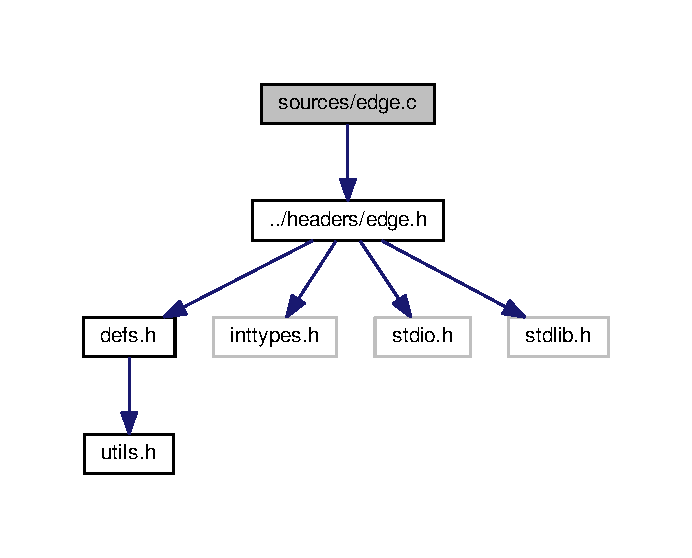
\includegraphics[width=332pt]{edge_8c__incl}
\end{center}
\end{figure}
\subsection*{Functions}
\begin{DoxyCompactItemize}
\item 
\hyperlink{edge_8h_ab4a642fc78a44ca8df119570b3288e13}{E\+D\+GE} \hyperlink{edge_8c_a15ac9743daa3a7d6ade50b68d6de86eb}{create\+\_\+edge} (uint32\+\_\+t edge\+\_\+id, \hyperlink{utils_8h_aa268a41a13430b18e933ed40207178d0}{D\+I\+R\+E\+C\+T\+I\+ON} dir)
\begin{DoxyCompactList}\small\item\em Function that creates an E\+D\+GE from a node id and a direction. \end{DoxyCompactList}\item 
uint32\+\_\+t \hyperlink{edge_8c_ad9aa111cad82e20619c31f7fc8cc8c96}{get\+\_\+neighbor\+\_\+id} (\hyperlink{edge_8h_ab4a642fc78a44ca8df119570b3288e13}{E\+D\+GE} e)
\begin{DoxyCompactList}\small\item\em Function that returns the neighbor id of an edge. \end{DoxyCompactList}\item 
\hyperlink{utils_8h_aa268a41a13430b18e933ed40207178d0}{D\+I\+R\+E\+C\+T\+I\+ON} \hyperlink{edge_8c_a1038dbe86b3582aa654a201c791b9293}{get\+\_\+direction} (\hyperlink{edge_8h_ab4a642fc78a44ca8df119570b3288e13}{E\+D\+GE} e)
\begin{DoxyCompactList}\small\item\em Function that returns the direction of an edge. \end{DoxyCompactList}\item 
\hyperlink{utils_8h_a32c27cc471df37f4fc818d65de0a56c4}{S\+T\+A\+T\+US} \hyperlink{edge_8c_afb1416581aec9a56ad9354e3826a9fd7}{set\+\_\+direction} (\hyperlink{edge_8h_ab4a642fc78a44ca8df119570b3288e13}{E\+D\+GE} $\ast$e, \hyperlink{utils_8h_aa268a41a13430b18e933ed40207178d0}{D\+I\+R\+E\+C\+T\+I\+ON} dir)
\begin{DoxyCompactList}\small\item\em Function that sets the direction of an edge. \end{DoxyCompactList}\item 
int \hyperlink{edge_8c_ac14fd9b58d75db6a3dba3b5f65baac8f}{comp\+\_\+edges} (const void $\ast$key, const void $\ast$e2)
\begin{DoxyCompactList}\small\item\em Function that compares to edges based on the neighbor ids. \end{DoxyCompactList}\item 
void \hyperlink{edge_8c_a4be4f5fd773a94c7a53773a54906ad02}{insert\+\_\+edge} (void $\ast$adj\+\_\+list, void $\ast$e, int pos)
\begin{DoxyCompactList}\small\item\em Function that inserts an edge in an adjacency lists. \end{DoxyCompactList}\item 
void \hyperlink{edge_8c_a41ae2473935226d4734adcb6e2c8ccaa}{print\+\_\+edge} (uint32\+\_\+t in, \hyperlink{edge_8h_ab4a642fc78a44ca8df119570b3288e13}{E\+D\+GE} e)
\begin{DoxyCompactList}\small\item\em Function prints an edge. \end{DoxyCompactList}\end{DoxyCompactItemize}


\subsection{Detailed Description}
This file contains the code that implements the functions defined in the header file \hyperlink{edge_8h}{edge.\+h}. Please refer to it to check the documentation. 

\begin{DoxyAuthor}{Author}
\+: Carlos Alfaro
\end{DoxyAuthor}
\begin{DoxyDate}{Date}
\+: 23-\/10-\/2017 
\end{DoxyDate}


\subsection{Function Documentation}
\mbox{\Hypertarget{edge_8c_ac14fd9b58d75db6a3dba3b5f65baac8f}\label{edge_8c_ac14fd9b58d75db6a3dba3b5f65baac8f}} 
\index{edge.\+c@{edge.\+c}!comp\+\_\+edges@{comp\+\_\+edges}}
\index{comp\+\_\+edges@{comp\+\_\+edges}!edge.\+c@{edge.\+c}}
\subsubsection{\texorpdfstring{comp\+\_\+edges()}{comp\_edges()}}
{\footnotesize\ttfamily int comp\+\_\+edges (\begin{DoxyParamCaption}\item[{const void $\ast$}]{e1,  }\item[{const void $\ast$}]{e2 }\end{DoxyParamCaption})}



Function that compares to edges based on the neighbor ids. 


\begin{DoxyParams}{Parameters}
{\em const} & void$\ast$ e1\+: First edge \\
\hline
{\em const} & void$\ast$ e2\+: Second edge\\
\hline
\end{DoxyParams}
\begin{DoxyReturn}{Returns}
int\+: a value less than, equal to or greater than 0 ~\newline
depending on whether e1 is smaller than, equal or greater ~\newline
than e2, respectively 
\end{DoxyReturn}
\mbox{\Hypertarget{edge_8c_a15ac9743daa3a7d6ade50b68d6de86eb}\label{edge_8c_a15ac9743daa3a7d6ade50b68d6de86eb}} 
\index{edge.\+c@{edge.\+c}!create\+\_\+edge@{create\+\_\+edge}}
\index{create\+\_\+edge@{create\+\_\+edge}!edge.\+c@{edge.\+c}}
\subsubsection{\texorpdfstring{create\+\_\+edge()}{create\_edge()}}
{\footnotesize\ttfamily \hyperlink{edge_8h_ab4a642fc78a44ca8df119570b3288e13}{E\+D\+GE} create\+\_\+edge (\begin{DoxyParamCaption}\item[{uint32\+\_\+t}]{edge\+\_\+id,  }\item[{\hyperlink{utils_8h_aa268a41a13430b18e933ed40207178d0}{D\+I\+R\+E\+C\+T\+I\+ON}}]{dir }\end{DoxyParamCaption})}



Function that creates an E\+D\+GE from a node id and a direction. 


\begin{DoxyParams}{Parameters}
{\em uint32\+\_\+t} & edge\+\_\+id\+: id of the neighbor node \\
\hline
{\em D\+I\+R\+E\+C\+T\+I\+ON} & dir\+: direction of the edge\\
\hline
\end{DoxyParams}
\begin{DoxyReturn}{Returns}
E\+D\+GE\+: the new created edge 
\end{DoxyReturn}
\mbox{\Hypertarget{edge_8c_a1038dbe86b3582aa654a201c791b9293}\label{edge_8c_a1038dbe86b3582aa654a201c791b9293}} 
\index{edge.\+c@{edge.\+c}!get\+\_\+direction@{get\+\_\+direction}}
\index{get\+\_\+direction@{get\+\_\+direction}!edge.\+c@{edge.\+c}}
\subsubsection{\texorpdfstring{get\+\_\+direction()}{get\_direction()}}
{\footnotesize\ttfamily \hyperlink{utils_8h_aa268a41a13430b18e933ed40207178d0}{D\+I\+R\+E\+C\+T\+I\+ON} get\+\_\+direction (\begin{DoxyParamCaption}\item[{\hyperlink{edge_8h_ab4a642fc78a44ca8df119570b3288e13}{E\+D\+GE}}]{e }\end{DoxyParamCaption})}



Function that returns the direction of an edge. 


\begin{DoxyParams}{Parameters}
{\em E\+D\+GE} & e\+: The edge\\
\hline
\end{DoxyParams}
\begin{DoxyReturn}{Returns}
D\+I\+R\+E\+C\+T\+I\+ON\+: The direction of the edge 
\end{DoxyReturn}
\mbox{\Hypertarget{edge_8c_ad9aa111cad82e20619c31f7fc8cc8c96}\label{edge_8c_ad9aa111cad82e20619c31f7fc8cc8c96}} 
\index{edge.\+c@{edge.\+c}!get\+\_\+neighbor\+\_\+id@{get\+\_\+neighbor\+\_\+id}}
\index{get\+\_\+neighbor\+\_\+id@{get\+\_\+neighbor\+\_\+id}!edge.\+c@{edge.\+c}}
\subsubsection{\texorpdfstring{get\+\_\+neighbor\+\_\+id()}{get\_neighbor\_id()}}
{\footnotesize\ttfamily uint32\+\_\+t get\+\_\+neighbor\+\_\+id (\begin{DoxyParamCaption}\item[{\hyperlink{edge_8h_ab4a642fc78a44ca8df119570b3288e13}{E\+D\+GE}}]{e }\end{DoxyParamCaption})}



Function that returns the neighbor id of an edge. 


\begin{DoxyParams}{Parameters}
{\em E\+D\+GE} & e\+: The edge\\
\hline
\end{DoxyParams}
\begin{DoxyReturn}{Returns}
uint32\+\_\+t\+: The neighbor id 
\end{DoxyReturn}
\mbox{\Hypertarget{edge_8c_a4be4f5fd773a94c7a53773a54906ad02}\label{edge_8c_a4be4f5fd773a94c7a53773a54906ad02}} 
\index{edge.\+c@{edge.\+c}!insert\+\_\+edge@{insert\+\_\+edge}}
\index{insert\+\_\+edge@{insert\+\_\+edge}!edge.\+c@{edge.\+c}}
\subsubsection{\texorpdfstring{insert\+\_\+edge()}{insert\_edge()}}
{\footnotesize\ttfamily void insert\+\_\+edge (\begin{DoxyParamCaption}\item[{void $\ast$}]{adj\+\_\+list,  }\item[{void $\ast$}]{e,  }\item[{int}]{pos }\end{DoxyParamCaption})}



Function that inserts an edge in an adjacency lists. 


\begin{DoxyParams}{Parameters}
{\em void$\ast$} & adj\+\_\+list\+: array where to insert the edge \\
\hline
{\em void$\ast$} & edge\+: Edge to insert \\
\hline
{\em int} & pos\+: The position where to insert\\
\hline
\end{DoxyParams}
\begin{DoxyReturn}{Returns}
None 
\end{DoxyReturn}
\mbox{\Hypertarget{edge_8c_a41ae2473935226d4734adcb6e2c8ccaa}\label{edge_8c_a41ae2473935226d4734adcb6e2c8ccaa}} 
\index{edge.\+c@{edge.\+c}!print\+\_\+edge@{print\+\_\+edge}}
\index{print\+\_\+edge@{print\+\_\+edge}!edge.\+c@{edge.\+c}}
\subsubsection{\texorpdfstring{print\+\_\+edge()}{print\_edge()}}
{\footnotesize\ttfamily void print\+\_\+edge (\begin{DoxyParamCaption}\item[{uint32\+\_\+t}]{in,  }\item[{\hyperlink{edge_8h_ab4a642fc78a44ca8df119570b3288e13}{E\+D\+GE}}]{e }\end{DoxyParamCaption})}



Function prints an edge. 


\begin{DoxyParams}{Parameters}
{\em uint32\+\_\+t} & in\+: the node id from where the node goes out \\
\hline
{\em E\+D\+GE} & e\+: The edge to print\\
\hline
\end{DoxyParams}
\begin{DoxyReturn}{Returns}
None 
\end{DoxyReturn}
\mbox{\Hypertarget{edge_8c_afb1416581aec9a56ad9354e3826a9fd7}\label{edge_8c_afb1416581aec9a56ad9354e3826a9fd7}} 
\index{edge.\+c@{edge.\+c}!set\+\_\+direction@{set\+\_\+direction}}
\index{set\+\_\+direction@{set\+\_\+direction}!edge.\+c@{edge.\+c}}
\subsubsection{\texorpdfstring{set\+\_\+direction()}{set\_direction()}}
{\footnotesize\ttfamily \hyperlink{utils_8h_a32c27cc471df37f4fc818d65de0a56c4}{S\+T\+A\+T\+US} set\+\_\+direction (\begin{DoxyParamCaption}\item[{\hyperlink{edge_8h_ab4a642fc78a44ca8df119570b3288e13}{E\+D\+GE} $\ast$}]{e,  }\item[{\hyperlink{utils_8h_aa268a41a13430b18e933ed40207178d0}{D\+I\+R\+E\+C\+T\+I\+ON}}]{dir }\end{DoxyParamCaption})}



Function that sets the direction of an edge. 


\begin{DoxyParams}{Parameters}
{\em E\+D\+GE} & e\+: The edge we want to modify \\
\hline
{\em D\+I\+R\+E\+C\+T\+I\+ON} & dir\+: The direction to set\\
\hline
\end{DoxyParams}
\begin{DoxyReturn}{Returns}
S\+T\+A\+T\+US\+: OK if the operation was successful~\newline
 E\+RR otherwise 
\end{DoxyReturn}

\hypertarget{graph_8c}{}\section{sources/graph.c File Reference}
\label{graph_8c}\index{sources/graph.\+c@{sources/graph.\+c}}


This file contains the code that implements the functions defined in the header file \hyperlink{graph_8h}{graph.\+h}. Please refer to it to check the documentation.  


{\ttfamily \#include \char`\"{}../headers/graph.\+h\char`\"{}}\newline
Include dependency graph for graph.\+c\+:
\nopagebreak
\begin{figure}[H]
\begin{center}
\leavevmode
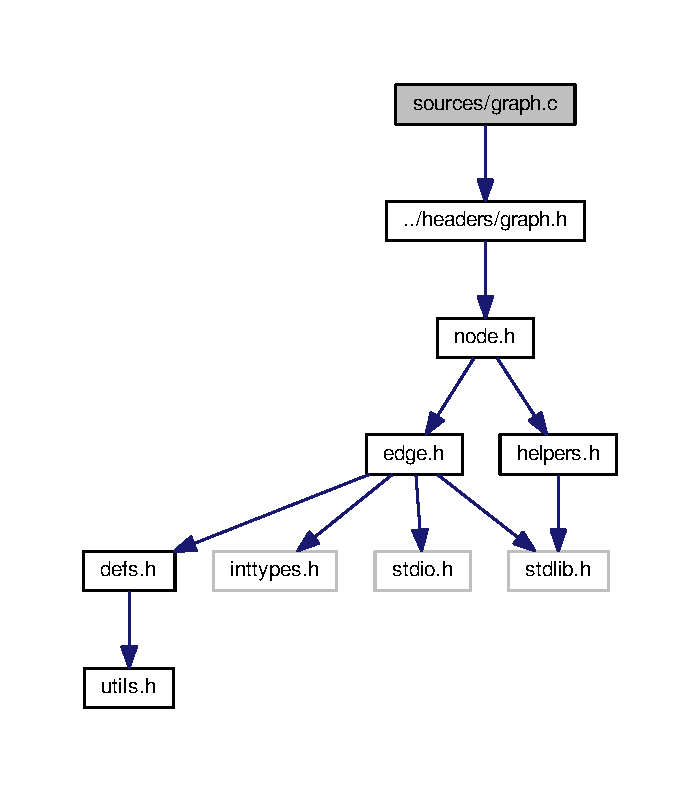
\includegraphics[width=336pt]{graph_8c__incl}
\end{center}
\end{figure}
\subsection*{Functions}
\begin{DoxyCompactItemize}
\item 
void \hyperlink{graph_8c_aa4ecaf8c04f3465eb1fd3c0a74927669}{set\+\_\+ordered} (\hyperlink{utils_8h_a3e5b8192e7d9ffaf3542f1210aec18dd}{B\+O\+OL} value)
\begin{DoxyCompactList}\small\item\em Function that sets the global variable ordered to a certain value passed as a parameter. \end{DoxyCompactList}\item 
\hyperlink{structGRAPH}{G\+R\+A\+PH} $\ast$ \hyperlink{graph_8c_a1e691638038900c9478325f5dbd66e0e}{read\+\_\+graph\+\_\+from\+\_\+file} (char $\ast$filename)
\begin{DoxyCompactList}\small\item\em Function that reads the file containing the graph information,~\newline
 and creates the \hyperlink{structGRAPH}{G\+R\+A\+PH} structure, returning a pointer to it. \end{DoxyCompactList}\item 
\hyperlink{utils_8h_a32c27cc471df37f4fc818d65de0a56c4}{S\+T\+A\+T\+US} \hyperlink{graph_8c_a00c645263fd09257dcc7d7f790a8a139}{insert\+\_\+node} (\hyperlink{structGRAPH}{G\+R\+A\+PH} $\ast$g, uint32\+\_\+t node\+\_\+id)
\begin{DoxyCompactList}\small\item\em Function that inserts a node in the graph. \end{DoxyCompactList}\item 
\hyperlink{utils_8h_a32c27cc471df37f4fc818d65de0a56c4}{S\+T\+A\+T\+US} \hyperlink{graph_8c_ac54e6c3dd8086e0d0054866fcb48c8fa}{add\+\_\+edge} (\hyperlink{structGRAPH}{G\+R\+A\+PH} $\ast$g, uint32\+\_\+t node\+\_\+id1, uint32\+\_\+t node\+\_\+id2, \hyperlink{utils_8h_aa268a41a13430b18e933ed40207178d0}{D\+I\+R\+E\+C\+T\+I\+ON} dir)
\begin{DoxyCompactList}\small\item\em Function that adds an edge to a certain node. To add an edge e,~\newline
we need to have the ids of the two nodes that the e connects; ant its ~\newline
direction. The function basically adds the edge to the adjacency list of~\newline
the node with id node\+\_\+id1, setting the neighbor id of the edge to node\+\_\+id2. \end{DoxyCompactList}\item 
\hyperlink{utils_8h_a3e5b8192e7d9ffaf3542f1210aec18dd}{B\+O\+OL} \hyperlink{graph_8c_a327ad76c2c67dc829facce47bb987de3}{node\+\_\+exists} (\hyperlink{structGRAPH}{G\+R\+A\+PH} $\ast$g, uint32\+\_\+t node\+\_\+id)
\begin{DoxyCompactList}\small\item\em Function that checks whether a node is present in a graph. \end{DoxyCompactList}\item 
int \hyperlink{graph_8c_a958ec048e564a498f7e2fb6eea436d35}{get\+\_\+node\+\_\+pos} (\hyperlink{structGRAPH}{G\+R\+A\+PH} $\ast$g, uint32\+\_\+t node\+\_\+id)
\begin{DoxyCompactList}\small\item\em Function that obtains the position of the node with id node\+\_\+id within the ~\newline
array of nodes of graph g. \end{DoxyCompactList}\item 
uint32\+\_\+t \hyperlink{graph_8c_ab655a5453feb3f96ed28d14dd192287b}{get\+\_\+num\+\_\+nodes} (const \hyperlink{structGRAPH}{G\+R\+A\+PH} $\ast$g)
\begin{DoxyCompactList}\small\item\em Function that obtains the number of nodes of a graph g. \end{DoxyCompactList}\item 
uint32\+\_\+t \hyperlink{graph_8c_ac472a365756f3728c133b4cba52127d3}{get\+\_\+num\+\_\+pairs} (const \hyperlink{structGRAPH}{G\+R\+A\+PH} $\ast$g)
\begin{DoxyCompactList}\small\item\em Function that obtains the number of pairs (u,v) of nodes in graph g. \end{DoxyCompactList}\item 
uint64\+\_\+t \hyperlink{graph_8c_a17c6c18decd7024d45439e01aa4f359e}{get\+\_\+num\+\_\+triples} (const \hyperlink{structGRAPH}{G\+R\+A\+PH} $\ast$g)
\begin{DoxyCompactList}\small\item\em Function that obtains the number of triples (u,v,w) of nodes in graph g. \end{DoxyCompactList}\item 
uint32\+\_\+t \hyperlink{graph_8c_a69902bced6cd88bc38dd7c863b367dfc}{get\+\_\+num\+\_\+edges} (const \hyperlink{structGRAPH}{G\+R\+A\+PH} $\ast$g)
\begin{DoxyCompactList}\small\item\em Function that obtains the number of edges of ha graph g. \end{DoxyCompactList}\item 
\hyperlink{structNODE}{N\+O\+DE} $\ast$ \hyperlink{graph_8c_a15242f86399df5a7fcac2127c5606461}{get\+\_\+node\+\_\+by\+\_\+pos} (const \hyperlink{structGRAPH}{G\+R\+A\+PH} $\ast$g, int pos)
\begin{DoxyCompactList}\small\item\em Function that obtains the node of graph g present in position pos. \end{DoxyCompactList}\item 
\hyperlink{structNODE}{N\+O\+DE} $\ast$ \hyperlink{graph_8c_a479b13695ab11c89b03a81cf70ca889b}{get\+\_\+node\+\_\+by\+\_\+id} (\hyperlink{structGRAPH}{G\+R\+A\+PH} $\ast$g, uint32\+\_\+t node\+\_\+id)
\begin{DoxyCompactList}\small\item\em Function that obtains the node of graph g that has id node\+\_\+id. \end{DoxyCompactList}\item 
void \hyperlink{graph_8c_a4d6f9793800397e068b0031d7ba42bba}{print\+\_\+graph} (\hyperlink{structGRAPH}{G\+R\+A\+PH} $\ast$g)
\begin{DoxyCompactList}\small\item\em Function that prints the information of graph. \end{DoxyCompactList}\item 
void \hyperlink{graph_8c_a496da63fdfc498a7e901f2a65a39ffe8}{destroy\+\_\+graph} (\hyperlink{structGRAPH}{G\+R\+A\+PH} $\ast$g)
\begin{DoxyCompactList}\small\item\em Function that destroys a graph, freeing the memory of its structures. \end{DoxyCompactList}\item 
\hyperlink{utils_8h_a32c27cc471df37f4fc818d65de0a56c4}{S\+T\+A\+T\+US} \hyperlink{graph_8c_a5aab9084b4ffec389343766cf27bf752}{convert\+\_\+graph} (\hyperlink{structGRAPH}{G\+R\+A\+PH} $\ast$g, \hyperlink{structNODE__DEVICE}{N\+O\+D\+E\+\_\+\+D\+E\+V\+I\+CE} $\ast$$\ast$nodes, \hyperlink{structEDGE__DEVICE}{E\+D\+G\+E\+\_\+\+D\+E\+V\+I\+CE} $\ast$$\ast$edges, uint32\+\_\+t $\ast$num\+\_\+nodes, uint32\+\_\+t $\ast$num\+\_\+edges)
\begin{DoxyCompactList}\small\item\em Function that, given a graph, constructs the array of nodes and edges,~\newline
 which is a suitable saving format for processing the graph in the device. \end{DoxyCompactList}\item 
\hyperlink{structTASK}{T\+A\+SK} $\ast$ \hyperlink{graph_8c_a918eb6777060cb3eecf14703db2b1b76}{create\+\_\+tasks\+\_\+array} (\hyperlink{structGRAPH}{G\+R\+A\+PH} $\ast$g, \hyperlink{structNODE__DEVICE}{N\+O\+D\+E\+\_\+\+D\+E\+V\+I\+CE} $\ast$nodes, uint32\+\_\+t $\ast$num\+\_\+tasks)
\begin{DoxyCompactList}\small\item\em Function that creates an array of tasks. \end{DoxyCompactList}\end{DoxyCompactItemize}
\subsection*{Variables}
\begin{DoxyCompactItemize}
\item 
\hyperlink{utils_8h_a3e5b8192e7d9ffaf3542f1210aec18dd}{B\+O\+OL} \hyperlink{graph_8c_aa94b0ac5dc0f8919227cda71fe50db38}{ordered}
\end{DoxyCompactItemize}


\subsection{Detailed Description}
This file contains the code that implements the functions defined in the header file \hyperlink{graph_8h}{graph.\+h}. Please refer to it to check the documentation. 

\begin{DoxyAuthor}{Author}
\+: Carlos Alfaro
\end{DoxyAuthor}
\begin{DoxyDate}{Date}
\+: 23-\/10-\/2017 
\end{DoxyDate}


\subsection{Function Documentation}
\mbox{\Hypertarget{graph_8c_ac54e6c3dd8086e0d0054866fcb48c8fa}\label{graph_8c_ac54e6c3dd8086e0d0054866fcb48c8fa}} 
\index{graph.\+c@{graph.\+c}!add\+\_\+edge@{add\+\_\+edge}}
\index{add\+\_\+edge@{add\+\_\+edge}!graph.\+c@{graph.\+c}}
\subsubsection{\texorpdfstring{add\+\_\+edge()}{add\_edge()}}
{\footnotesize\ttfamily \hyperlink{utils_8h_a32c27cc471df37f4fc818d65de0a56c4}{S\+T\+A\+T\+US} add\+\_\+edge (\begin{DoxyParamCaption}\item[{\hyperlink{structGRAPH}{G\+R\+A\+PH} $\ast$}]{g,  }\item[{uint32\+\_\+t}]{node\+\_\+id1,  }\item[{uint32\+\_\+t}]{node\+\_\+id2,  }\item[{\hyperlink{utils_8h_aa268a41a13430b18e933ed40207178d0}{D\+I\+R\+E\+C\+T\+I\+ON}}]{dir }\end{DoxyParamCaption})}



Function that adds an edge to a certain node. To add an edge e,~\newline
we need to have the ids of the two nodes that the e connects; ant its ~\newline
direction. The function basically adds the edge to the adjacency list of~\newline
the node with id node\+\_\+id1, setting the neighbor id of the edge to node\+\_\+id2. 


\begin{DoxyParams}{Parameters}
{\em G\+R\+A\+P\+H$\ast$} & g\+: The graph in which we want to add the edge \\
\hline
{\em uint32\+\_\+t} & node\+\_\+id1\+: The id of one of the nodes of the edge \\
\hline
{\em uint32\+\_\+t} & node\+\_\+id2\+: The id of the other id \\
\hline
{\em D\+I\+R\+E\+C\+T\+I\+ON} & dir\+: The direction of the edge\+:  if it goes from id1 to id2.~\newline
 O\+U\+T\+\_\+\+IN if it goes from id2 to id1.\\
\hline
\end{DoxyParams}
\begin{DoxyReturn}{Returns}
S\+T\+A\+T\+US\+: OK if the insertion was successful. E\+RR otherwise 
\end{DoxyReturn}
\mbox{\Hypertarget{graph_8c_a5aab9084b4ffec389343766cf27bf752}\label{graph_8c_a5aab9084b4ffec389343766cf27bf752}} 
\index{graph.\+c@{graph.\+c}!convert\+\_\+graph@{convert\+\_\+graph}}
\index{convert\+\_\+graph@{convert\+\_\+graph}!graph.\+c@{graph.\+c}}
\subsubsection{\texorpdfstring{convert\+\_\+graph()}{convert\_graph()}}
{\footnotesize\ttfamily \hyperlink{utils_8h_a32c27cc471df37f4fc818d65de0a56c4}{S\+T\+A\+T\+US} convert\+\_\+graph (\begin{DoxyParamCaption}\item[{\hyperlink{structGRAPH}{G\+R\+A\+PH} $\ast$}]{g,  }\item[{\hyperlink{structNODE__DEVICE}{N\+O\+D\+E\+\_\+\+D\+E\+V\+I\+CE} $\ast$$\ast$}]{nodes,  }\item[{\hyperlink{structEDGE__DEVICE}{E\+D\+G\+E\+\_\+\+D\+E\+V\+I\+CE} $\ast$$\ast$}]{edges,  }\item[{uint32\+\_\+t $\ast$}]{num\+\_\+nodes,  }\item[{uint32\+\_\+t $\ast$}]{num\+\_\+edges }\end{DoxyParamCaption})}



Function that, given a graph, constructs the array of nodes and edges,~\newline
 which is a suitable saving format for processing the graph in the device. 


\begin{DoxyParams}{Parameters}
{\em G\+R\+A\+P\+H$\ast$} & g\+: the graph to convert \\
\hline
{\em N\+O\+D\+E\+\_\+\+D\+E\+V\+I\+C\+E$\ast$$\ast$} & nodes\+: A pointer to the array of nodes (to be filled) \\
\hline
{\em E\+D\+G\+E\+\_\+\+D\+E\+V\+I\+C\+E$\ast$$\ast$} & edges\+: A pointer to the array of edges (to be filled) \\
\hline
{\em uint32\+\_\+t$\ast$} & num\+\_\+nodes\+: The number of nodes, (to be filled) \\
\hline
{\em uint32\+\_\+t$\ast$} & num\+\_\+edges\+: The number of edges (to be filled)\\
\hline
\end{DoxyParams}
\begin{DoxyReturn}{Returns}
S\+T\+A\+T\+US\+: OK if the arrays were constructed correctly, E\+RR otherwise 
\end{DoxyReturn}
\mbox{\Hypertarget{graph_8c_a918eb6777060cb3eecf14703db2b1b76}\label{graph_8c_a918eb6777060cb3eecf14703db2b1b76}} 
\index{graph.\+c@{graph.\+c}!create\+\_\+tasks\+\_\+array@{create\+\_\+tasks\+\_\+array}}
\index{create\+\_\+tasks\+\_\+array@{create\+\_\+tasks\+\_\+array}!graph.\+c@{graph.\+c}}
\subsubsection{\texorpdfstring{create\+\_\+tasks\+\_\+array()}{create\_tasks\_array()}}
{\footnotesize\ttfamily \hyperlink{structTASK}{T\+A\+SK}$\ast$ create\+\_\+tasks\+\_\+array (\begin{DoxyParamCaption}\item[{\hyperlink{structGRAPH}{G\+R\+A\+PH} $\ast$}]{g,  }\item[{\hyperlink{structNODE__DEVICE}{N\+O\+D\+E\+\_\+\+D\+E\+V\+I\+CE} $\ast$}]{nodes,  }\item[{uint32\+\_\+t $\ast$}]{num\+\_\+tasks }\end{DoxyParamCaption})}



Function that creates an array of tasks. 


\begin{DoxyParams}{Parameters}
{\em G\+R\+A\+P\+H$\ast$} & g\+: the graph \\
\hline
{\em N\+O\+D\+E\+\_\+\+D\+E\+V\+I\+C\+E$\ast$} & nodes\+: The array of nodes \\
\hline
{\em uint32\+\_\+t$\ast$} & num\+\_\+tasks\+: The number of tasks (to be filled)\\
\hline
\end{DoxyParams}
\begin{DoxyReturn}{Returns}
T\+A\+S\+K$\ast$\+: The array of tasks just created 
\end{DoxyReturn}
\mbox{\Hypertarget{graph_8c_a496da63fdfc498a7e901f2a65a39ffe8}\label{graph_8c_a496da63fdfc498a7e901f2a65a39ffe8}} 
\index{graph.\+c@{graph.\+c}!destroy\+\_\+graph@{destroy\+\_\+graph}}
\index{destroy\+\_\+graph@{destroy\+\_\+graph}!graph.\+c@{graph.\+c}}
\subsubsection{\texorpdfstring{destroy\+\_\+graph()}{destroy\_graph()}}
{\footnotesize\ttfamily void destroy\+\_\+graph (\begin{DoxyParamCaption}\item[{\hyperlink{structGRAPH}{G\+R\+A\+PH} $\ast$}]{g }\end{DoxyParamCaption})}



Function that destroys a graph, freeing the memory of its structures. 


\begin{DoxyParams}{Parameters}
{\em G\+R\+A\+P\+H$\ast$} & g\+: the graph to destroy\\
\hline
\end{DoxyParams}
\begin{DoxyReturn}{Returns}
none 
\end{DoxyReturn}
\mbox{\Hypertarget{graph_8c_a479b13695ab11c89b03a81cf70ca889b}\label{graph_8c_a479b13695ab11c89b03a81cf70ca889b}} 
\index{graph.\+c@{graph.\+c}!get\+\_\+node\+\_\+by\+\_\+id@{get\+\_\+node\+\_\+by\+\_\+id}}
\index{get\+\_\+node\+\_\+by\+\_\+id@{get\+\_\+node\+\_\+by\+\_\+id}!graph.\+c@{graph.\+c}}
\subsubsection{\texorpdfstring{get\+\_\+node\+\_\+by\+\_\+id()}{get\_node\_by\_id()}}
{\footnotesize\ttfamily \hyperlink{structNODE}{N\+O\+DE}$\ast$ get\+\_\+node\+\_\+by\+\_\+id (\begin{DoxyParamCaption}\item[{\hyperlink{structGRAPH}{G\+R\+A\+PH} $\ast$}]{g,  }\item[{uint32\+\_\+t}]{node\+\_\+id }\end{DoxyParamCaption})}



Function that obtains the node of graph g that has id node\+\_\+id. 


\begin{DoxyParams}{Parameters}
{\em G\+R\+A\+P\+H$\ast$} & g\+: The graph im which to search uint32\+\_\+t node\+\_\+id\+: The position of the node we want to obtain\\
\hline
\end{DoxyParams}
\begin{DoxyReturn}{Returns}
N\+O\+D\+E$\ast$ the node we were looking for 
\end{DoxyReturn}
\mbox{\Hypertarget{graph_8c_a15242f86399df5a7fcac2127c5606461}\label{graph_8c_a15242f86399df5a7fcac2127c5606461}} 
\index{graph.\+c@{graph.\+c}!get\+\_\+node\+\_\+by\+\_\+pos@{get\+\_\+node\+\_\+by\+\_\+pos}}
\index{get\+\_\+node\+\_\+by\+\_\+pos@{get\+\_\+node\+\_\+by\+\_\+pos}!graph.\+c@{graph.\+c}}
\subsubsection{\texorpdfstring{get\+\_\+node\+\_\+by\+\_\+pos()}{get\_node\_by\_pos()}}
{\footnotesize\ttfamily \hyperlink{structNODE}{N\+O\+DE}$\ast$ get\+\_\+node\+\_\+by\+\_\+pos (\begin{DoxyParamCaption}\item[{const \hyperlink{structGRAPH}{G\+R\+A\+PH} $\ast$}]{g,  }\item[{int}]{pos }\end{DoxyParamCaption})}



Function that obtains the node of graph g present in position pos. 


\begin{DoxyParams}{Parameters}
{\em G\+R\+A\+P\+H$\ast$} & g\+: The graph in which to search \\
\hline
{\em int} & pos\+: The position of the node we want to obtain\\
\hline
\end{DoxyParams}
\begin{DoxyReturn}{Returns}
N\+O\+D\+E$\ast$ the node we were looking for 
\end{DoxyReturn}
\mbox{\Hypertarget{graph_8c_a958ec048e564a498f7e2fb6eea436d35}\label{graph_8c_a958ec048e564a498f7e2fb6eea436d35}} 
\index{graph.\+c@{graph.\+c}!get\+\_\+node\+\_\+pos@{get\+\_\+node\+\_\+pos}}
\index{get\+\_\+node\+\_\+pos@{get\+\_\+node\+\_\+pos}!graph.\+c@{graph.\+c}}
\subsubsection{\texorpdfstring{get\+\_\+node\+\_\+pos()}{get\_node\_pos()}}
{\footnotesize\ttfamily int get\+\_\+node\+\_\+pos (\begin{DoxyParamCaption}\item[{\hyperlink{structGRAPH}{G\+R\+A\+PH} $\ast$}]{g,  }\item[{uint32\+\_\+t}]{node\+\_\+id }\end{DoxyParamCaption})}



Function that obtains the position of the node with id node\+\_\+id within the ~\newline
array of nodes of graph g. 


\begin{DoxyParams}{Parameters}
{\em G\+R\+A\+P\+H$\ast$} & g\+: The graph in which we want to search the position of the node. \\
\hline
{\em uint32\+\_\+t} & node\+\_\+id\+: The id of the node we want to find the position of.\\
\hline
\end{DoxyParams}
\begin{DoxyReturn}{Returns}
S\+T\+A\+T\+US\+: int the position in which the node is stored, if the node is actually present~\newline
 -\/1 if the node is not found. 
\end{DoxyReturn}
\mbox{\Hypertarget{graph_8c_a69902bced6cd88bc38dd7c863b367dfc}\label{graph_8c_a69902bced6cd88bc38dd7c863b367dfc}} 
\index{graph.\+c@{graph.\+c}!get\+\_\+num\+\_\+edges@{get\+\_\+num\+\_\+edges}}
\index{get\+\_\+num\+\_\+edges@{get\+\_\+num\+\_\+edges}!graph.\+c@{graph.\+c}}
\subsubsection{\texorpdfstring{get\+\_\+num\+\_\+edges()}{get\_num\_edges()}}
{\footnotesize\ttfamily uint32\+\_\+t get\+\_\+num\+\_\+edges (\begin{DoxyParamCaption}\item[{const \hyperlink{structGRAPH}{G\+R\+A\+PH} $\ast$}]{g }\end{DoxyParamCaption})}



Function that obtains the number of edges of ha graph g. 


\begin{DoxyParams}{Parameters}
{\em const} & G\+R\+A\+P\+H$\ast$ g\+: The graph\\
\hline
\end{DoxyParams}
\begin{DoxyReturn}{Returns}
uint32\+\_\+t the number of edges of the graph 
\end{DoxyReturn}
\mbox{\Hypertarget{graph_8c_ab655a5453feb3f96ed28d14dd192287b}\label{graph_8c_ab655a5453feb3f96ed28d14dd192287b}} 
\index{graph.\+c@{graph.\+c}!get\+\_\+num\+\_\+nodes@{get\+\_\+num\+\_\+nodes}}
\index{get\+\_\+num\+\_\+nodes@{get\+\_\+num\+\_\+nodes}!graph.\+c@{graph.\+c}}
\subsubsection{\texorpdfstring{get\+\_\+num\+\_\+nodes()}{get\_num\_nodes()}}
{\footnotesize\ttfamily uint32\+\_\+t get\+\_\+num\+\_\+nodes (\begin{DoxyParamCaption}\item[{const \hyperlink{structGRAPH}{G\+R\+A\+PH} $\ast$}]{g }\end{DoxyParamCaption})}



Function that obtains the number of nodes of a graph g. 


\begin{DoxyParams}{Parameters}
{\em G\+R\+A\+P\+H$\ast$} & g\+: The graph\\
\hline
\end{DoxyParams}
\begin{DoxyReturn}{Returns}
uint32\+\_\+t the number of nodes of the graph 
\end{DoxyReturn}
\mbox{\Hypertarget{graph_8c_ac472a365756f3728c133b4cba52127d3}\label{graph_8c_ac472a365756f3728c133b4cba52127d3}} 
\index{graph.\+c@{graph.\+c}!get\+\_\+num\+\_\+pairs@{get\+\_\+num\+\_\+pairs}}
\index{get\+\_\+num\+\_\+pairs@{get\+\_\+num\+\_\+pairs}!graph.\+c@{graph.\+c}}
\subsubsection{\texorpdfstring{get\+\_\+num\+\_\+pairs()}{get\_num\_pairs()}}
{\footnotesize\ttfamily uint32\+\_\+t get\+\_\+num\+\_\+pairs (\begin{DoxyParamCaption}\item[{const \hyperlink{structGRAPH}{G\+R\+A\+PH} $\ast$}]{g }\end{DoxyParamCaption})}



Function that obtains the number of pairs (u,v) of nodes in graph g. 


\begin{DoxyParams}{Parameters}
{\em G\+R\+A\+P\+H$\ast$} & g\+: The graph\\
\hline
\end{DoxyParams}
\begin{DoxyReturn}{Returns}
uint32\+\_\+t the number of pairs in the graph 
\end{DoxyReturn}
\mbox{\Hypertarget{graph_8c_a17c6c18decd7024d45439e01aa4f359e}\label{graph_8c_a17c6c18decd7024d45439e01aa4f359e}} 
\index{graph.\+c@{graph.\+c}!get\+\_\+num\+\_\+triples@{get\+\_\+num\+\_\+triples}}
\index{get\+\_\+num\+\_\+triples@{get\+\_\+num\+\_\+triples}!graph.\+c@{graph.\+c}}
\subsubsection{\texorpdfstring{get\+\_\+num\+\_\+triples()}{get\_num\_triples()}}
{\footnotesize\ttfamily uint64\+\_\+t get\+\_\+num\+\_\+triples (\begin{DoxyParamCaption}\item[{const \hyperlink{structGRAPH}{G\+R\+A\+PH} $\ast$}]{g }\end{DoxyParamCaption})}



Function that obtains the number of triples (u,v,w) of nodes in graph g. 


\begin{DoxyParams}{Parameters}
{\em G\+R\+A\+P\+H$\ast$} & g\+: The graph\\
\hline
\end{DoxyParams}
\begin{DoxyReturn}{Returns}
uint32\+\_\+t the number of triples in the graph 
\end{DoxyReturn}
\mbox{\Hypertarget{graph_8c_a00c645263fd09257dcc7d7f790a8a139}\label{graph_8c_a00c645263fd09257dcc7d7f790a8a139}} 
\index{graph.\+c@{graph.\+c}!insert\+\_\+node@{insert\+\_\+node}}
\index{insert\+\_\+node@{insert\+\_\+node}!graph.\+c@{graph.\+c}}
\subsubsection{\texorpdfstring{insert\+\_\+node()}{insert\_node()}}
{\footnotesize\ttfamily \hyperlink{utils_8h_a32c27cc471df37f4fc818d65de0a56c4}{S\+T\+A\+T\+US} insert\+\_\+node (\begin{DoxyParamCaption}\item[{\hyperlink{structGRAPH}{G\+R\+A\+PH} $\ast$}]{g,  }\item[{uint32\+\_\+t}]{node\+\_\+id }\end{DoxyParamCaption})}



Function that inserts a node in the graph. 


\begin{DoxyParams}{Parameters}
{\em G\+R\+A\+P\+H$\ast$} & g\+: The graph in which to insert \\
\hline
{\em uint32\+\_\+t} & node\+\_\+id\+: The id of the node we want to insert\\
\hline
\end{DoxyParams}
\begin{DoxyReturn}{Returns}
S\+T\+A\+T\+US\+: OK if the insertion was successful. E\+RR otherwise 
\end{DoxyReturn}
\mbox{\Hypertarget{graph_8c_a327ad76c2c67dc829facce47bb987de3}\label{graph_8c_a327ad76c2c67dc829facce47bb987de3}} 
\index{graph.\+c@{graph.\+c}!node\+\_\+exists@{node\+\_\+exists}}
\index{node\+\_\+exists@{node\+\_\+exists}!graph.\+c@{graph.\+c}}
\subsubsection{\texorpdfstring{node\+\_\+exists()}{node\_exists()}}
{\footnotesize\ttfamily \hyperlink{utils_8h_a3e5b8192e7d9ffaf3542f1210aec18dd}{B\+O\+OL} node\+\_\+exists (\begin{DoxyParamCaption}\item[{\hyperlink{structGRAPH}{G\+R\+A\+PH} $\ast$}]{g,  }\item[{uint32\+\_\+t}]{node\+\_\+id }\end{DoxyParamCaption})}



Function that checks whether a node is present in a graph. 


\begin{DoxyParams}{Parameters}
{\em G\+R\+A\+P\+H$\ast$} & g\+: The graph in which to search. \\
\hline
{\em uint32\+\_\+t} & node\+\_\+id\+: The id of the node we want to search.\\
\hline
\end{DoxyParams}
\begin{DoxyReturn}{Returns}
B\+O\+OL\+: T\+R\+UE if the node is found.~\newline
 F\+A\+L\+SE otherwise 
\end{DoxyReturn}
\mbox{\Hypertarget{graph_8c_a4d6f9793800397e068b0031d7ba42bba}\label{graph_8c_a4d6f9793800397e068b0031d7ba42bba}} 
\index{graph.\+c@{graph.\+c}!print\+\_\+graph@{print\+\_\+graph}}
\index{print\+\_\+graph@{print\+\_\+graph}!graph.\+c@{graph.\+c}}
\subsubsection{\texorpdfstring{print\+\_\+graph()}{print\_graph()}}
{\footnotesize\ttfamily void print\+\_\+graph (\begin{DoxyParamCaption}\item[{\hyperlink{structGRAPH}{G\+R\+A\+PH} $\ast$}]{g }\end{DoxyParamCaption})}



Function that prints the information of graph. 


\begin{DoxyParams}{Parameters}
{\em G\+R\+A\+P\+H$\ast$} & g\+: The graph to print\\
\hline
\end{DoxyParams}
\begin{DoxyReturn}{Returns}
none 
\end{DoxyReturn}
\mbox{\Hypertarget{graph_8c_a1e691638038900c9478325f5dbd66e0e}\label{graph_8c_a1e691638038900c9478325f5dbd66e0e}} 
\index{graph.\+c@{graph.\+c}!read\+\_\+graph\+\_\+from\+\_\+file@{read\+\_\+graph\+\_\+from\+\_\+file}}
\index{read\+\_\+graph\+\_\+from\+\_\+file@{read\+\_\+graph\+\_\+from\+\_\+file}!graph.\+c@{graph.\+c}}
\subsubsection{\texorpdfstring{read\+\_\+graph\+\_\+from\+\_\+file()}{read\_graph\_from\_file()}}
{\footnotesize\ttfamily \hyperlink{structGRAPH}{G\+R\+A\+PH}$\ast$ read\+\_\+graph\+\_\+from\+\_\+file (\begin{DoxyParamCaption}\item[{char $\ast$}]{filename }\end{DoxyParamCaption})}



Function that reads the file containing the graph information,~\newline
 and creates the \hyperlink{structGRAPH}{G\+R\+A\+PH} structure, returning a pointer to it. 


\begin{DoxyParams}{Parameters}
{\em char$\ast$} & filename\+: The name of the file to read.\\
\hline
\end{DoxyParams}
\begin{DoxyReturn}{Returns}
N\+O\+D\+E$\ast$\+: A pointer to the just created. 
\end{DoxyReturn}
\mbox{\Hypertarget{graph_8c_aa4ecaf8c04f3465eb1fd3c0a74927669}\label{graph_8c_aa4ecaf8c04f3465eb1fd3c0a74927669}} 
\index{graph.\+c@{graph.\+c}!set\+\_\+ordered@{set\+\_\+ordered}}
\index{set\+\_\+ordered@{set\+\_\+ordered}!graph.\+c@{graph.\+c}}
\subsubsection{\texorpdfstring{set\+\_\+ordered()}{set\_ordered()}}
{\footnotesize\ttfamily void set\+\_\+ordered (\begin{DoxyParamCaption}\item[{\hyperlink{utils_8h_a3e5b8192e7d9ffaf3542f1210aec18dd}{B\+O\+OL}}]{value }\end{DoxyParamCaption})}



Function that sets the global variable ordered to a certain value passed as a parameter. 


\begin{DoxyParams}{Parameters}
{\em B\+O\+OL} & value\+: The boolean value we want to set.\\
\hline
\end{DoxyParams}
\begin{DoxyReturn}{Returns}
\+: None 
\end{DoxyReturn}


\subsection{Variable Documentation}
\mbox{\Hypertarget{graph_8c_aa94b0ac5dc0f8919227cda71fe50db38}\label{graph_8c_aa94b0ac5dc0f8919227cda71fe50db38}} 
\index{graph.\+c@{graph.\+c}!ordered@{ordered}}
\index{ordered@{ordered}!graph.\+c@{graph.\+c}}
\subsubsection{\texorpdfstring{ordered}{ordered}}
{\footnotesize\ttfamily \hyperlink{utils_8h_a3e5b8192e7d9ffaf3542f1210aec18dd}{B\+O\+OL} ordered}

Flag to determine whether the data managed has to be ordered or not 
\hypertarget{helpers_8c}{}\section{sources/helpers.c File Reference}
\label{helpers_8c}\index{sources/helpers.\+c@{sources/helpers.\+c}}


This file contains the code that implements the functions defined in the header file \hyperlink{helpers_8h}{helpers.\+h}. Please refer to it to check the documentation.  


{\ttfamily \#include \char`\"{}../headers/helpers.\+h\char`\"{}}\newline
Include dependency graph for helpers.\+c\+:
\nopagebreak
\begin{figure}[H]
\begin{center}
\leavevmode
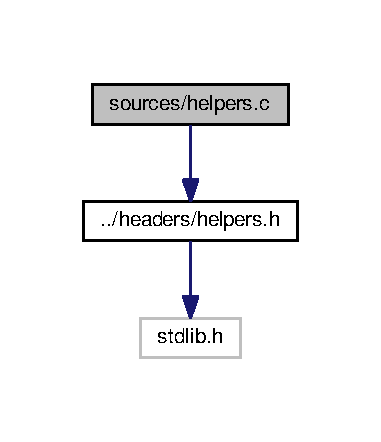
\includegraphics[width=183pt]{helpers_8c__incl}
\end{center}
\end{figure}
\subsection*{Functions}
\begin{DoxyCompactItemize}
\item 
int \hyperlink{helpers_8c_acc35bd25a8a468de5eecd3ac86cad3d6}{linear\+\_\+search} (void $\ast$table, int num\+\_\+elems, size\+\_\+t size, void $\ast$key, int($\ast$comp)(const void $\ast$arg1, const void $\ast$arg2))
\begin{DoxyCompactList}\small\item\em Function that performs linear search over an unordered array. \end{DoxyCompactList}\item 
int \hyperlink{helpers_8c_a179fbd21d334a48da1fb846b53dd04f7}{binary\+\_\+search} (void $\ast$table, int first, int last, size\+\_\+t size, void $\ast$key, int($\ast$comp)(const void $\ast$arg1, const void $\ast$arg2))
\begin{DoxyCompactList}\small\item\em Function that performs binary search over an ordered array. \end{DoxyCompactList}\item 
void \hyperlink{helpers_8c_abf6d4a9fcd1142a7b5bd256d278f8745}{insert\+\_\+sort} (void $\ast$table, size\+\_\+t size, int nmemb, void $\ast$elem, void $\ast$key, int($\ast$comp)(const void $\ast$arg1, const void $\ast$arg2), void($\ast$insert)(void $\ast$table, void $\ast$key, int pos))
\begin{DoxyCompactList}\small\item\em Function that performs the insertion sort (inner loop of the algorithm) \end{DoxyCompactList}\end{DoxyCompactItemize}


\subsection{Detailed Description}
This file contains the code that implements the functions defined in the header file \hyperlink{helpers_8h}{helpers.\+h}. Please refer to it to check the documentation. 

\begin{DoxyAuthor}{Author}
\+: Carlos Alfaro
\end{DoxyAuthor}
\begin{DoxyDate}{Date}
\+: 19-\/10-\/2017 
\end{DoxyDate}


\subsection{Function Documentation}
\mbox{\Hypertarget{helpers_8c_a179fbd21d334a48da1fb846b53dd04f7}\label{helpers_8c_a179fbd21d334a48da1fb846b53dd04f7}} 
\index{helpers.\+c@{helpers.\+c}!binary\+\_\+search@{binary\+\_\+search}}
\index{binary\+\_\+search@{binary\+\_\+search}!helpers.\+c@{helpers.\+c}}
\subsubsection{\texorpdfstring{binary\+\_\+search()}{binary\_search()}}
{\footnotesize\ttfamily int binary\+\_\+search (\begin{DoxyParamCaption}\item[{void $\ast$}]{table,  }\item[{int}]{first,  }\item[{int}]{last,  }\item[{size\+\_\+t}]{size,  }\item[{void $\ast$}]{key,  }\item[{int($\ast$)(const void $\ast$arg1, const void $\ast$arg2)}]{comp }\end{DoxyParamCaption})}



Function that performs binary search over an ordered array. 


\begin{DoxyParams}{Parameters}
{\em void$\ast$} & table\+: The array in which to perform the search \\
\hline
{\em int} & first\+: the first index of the table \\
\hline
{\em int} & last\+: the last index of the table \\
\hline
{\em size\+\_\+t} & size\+: size in bytes of each of the elements of the array \\
\hline
{\em void$\ast$} & key\+: The key to search within the array \\
\hline
{\em int} & ({\itshape comp) (const void} arg1, const void$\ast$ arg2)\+: pointer to the campare function\\
\hline
\end{DoxyParams}
\begin{DoxyReturn}{Returns}
int the position in which the key is stored, if it is found~\newline
 -\/1 otherwise 
\end{DoxyReturn}
\mbox{\Hypertarget{helpers_8c_abf6d4a9fcd1142a7b5bd256d278f8745}\label{helpers_8c_abf6d4a9fcd1142a7b5bd256d278f8745}} 
\index{helpers.\+c@{helpers.\+c}!insert\+\_\+sort@{insert\+\_\+sort}}
\index{insert\+\_\+sort@{insert\+\_\+sort}!helpers.\+c@{helpers.\+c}}
\subsubsection{\texorpdfstring{insert\+\_\+sort()}{insert\_sort()}}
{\footnotesize\ttfamily void insert\+\_\+sort (\begin{DoxyParamCaption}\item[{void $\ast$}]{table,  }\item[{size\+\_\+t}]{size,  }\item[{int}]{nmemb,  }\item[{void $\ast$}]{elem,  }\item[{void $\ast$}]{key,  }\item[{int($\ast$)(const void $\ast$arg1, const void $\ast$arg2)}]{comp,  }\item[{void($\ast$)(void $\ast$table, void $\ast$key, int pos)}]{insert }\end{DoxyParamCaption})}



Function that performs the insertion sort (inner loop of the algorithm) 


\begin{DoxyParams}{Parameters}
{\em void$\ast$} & table\+: The array in which to perform the insertion \\
\hline
{\em size\+\_\+t} & size\+: size in bytes of each of the elements of the array \\
\hline
{\em int} & nmemb\+: Number of elements present in the array \\
\hline
{\em void$\ast$} & elem\+: element to insert \\
\hline
{\em void} & $\ast$key\+: key associated to the element, useful to compare to other elements \\
\hline
{\em int} & ({\itshape comp) (const void} arg1, const void$\ast$ arg2)\+: pointer to the compare function void ({\itshape insert)(void} table, void$\ast$ key, int pos)\+:pointer to the insertion function\\
\hline
\end{DoxyParams}
\begin{DoxyReturn}{Returns}
int the position in which the key is stored, if it is found -\/1 otherwise 
\end{DoxyReturn}
\mbox{\Hypertarget{helpers_8c_acc35bd25a8a468de5eecd3ac86cad3d6}\label{helpers_8c_acc35bd25a8a468de5eecd3ac86cad3d6}} 
\index{helpers.\+c@{helpers.\+c}!linear\+\_\+search@{linear\+\_\+search}}
\index{linear\+\_\+search@{linear\+\_\+search}!helpers.\+c@{helpers.\+c}}
\subsubsection{\texorpdfstring{linear\+\_\+search()}{linear\_search()}}
{\footnotesize\ttfamily int linear\+\_\+search (\begin{DoxyParamCaption}\item[{void $\ast$}]{table,  }\item[{int}]{num\+\_\+elems,  }\item[{size\+\_\+t}]{size,  }\item[{void $\ast$}]{key,  }\item[{int($\ast$)(const void $\ast$arg1, const void $\ast$arg2)}]{comp }\end{DoxyParamCaption})}



Function that performs linear search over an unordered array. 


\begin{DoxyParams}{Parameters}
{\em void$\ast$} & table\+: The array in which to perform the search \\
\hline
{\em int} & num\+\_\+elems\+: Number of elements in the array \\
\hline
{\em size\+\_\+t} & size\+: size in bytes of each of the elements of the array \\
\hline
{\em void$\ast$} & key\+: The key to search within the array \\
\hline
{\em int} & ({\itshape comp) (const void} arg1, const void$\ast$ arg2)\+: pointer to the campare function\\
\hline
\end{DoxyParams}
\begin{DoxyReturn}{Returns}
int the position in which the key is stored, if it is found~\newline
 -\/1 otherwise 
\end{DoxyReturn}

\hypertarget{main__parallel_8c}{}\section{sources/main\+\_\+parallel.c File Reference}
\label{main__parallel_8c}\index{sources/main\+\_\+parallel.\+c@{sources/main\+\_\+parallel.\+c}}


This is the main program of the Open\+CL application. It executes a user-\/specified accelerated version of triad census algorithm and displays results and execution performances depending on the parameters passed to the program.  


{\ttfamily \#include \char`\"{}../headers/aux\+\_\+opencl.\+h\char`\"{}}\newline
{\ttfamily \#include $<$getopt.\+h$>$}\newline
{\ttfamily \#include $<$sys/time.\+h$>$}\newline
Include dependency graph for main\+\_\+parallel.\+c\+:
\nopagebreak
\begin{figure}[H]
\begin{center}
\leavevmode
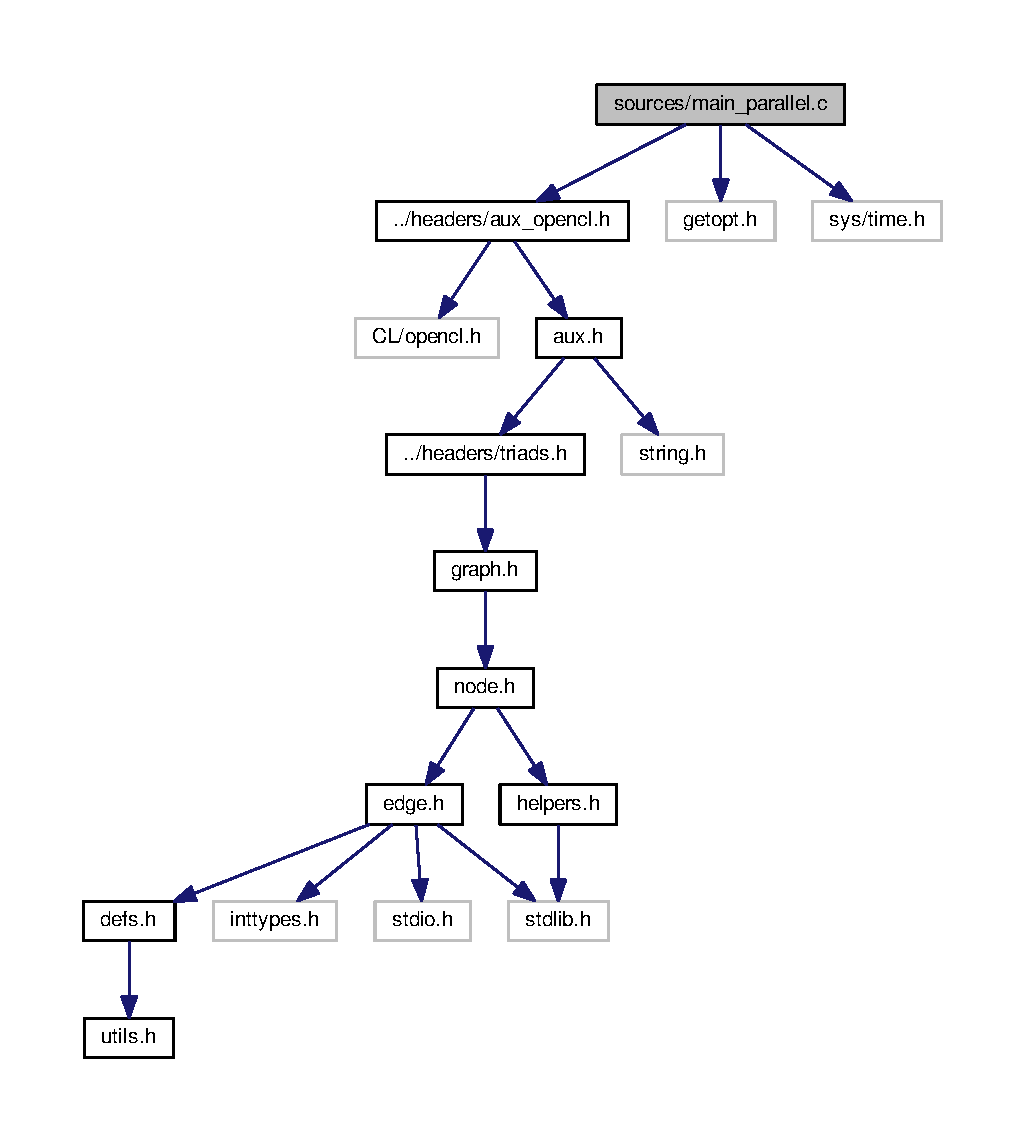
\includegraphics[width=350pt]{main__parallel_8c__incl}
\end{center}
\end{figure}
\subsection*{Functions}
\begin{DoxyCompactItemize}
\item 
\mbox{\Hypertarget{main__parallel_8c_a6d85d03371e68248c491c443a737c76f}\label{main__parallel_8c_a6d85d03371e68248c491c443a737c76f}} 
void {\bfseries display\+\_\+help} (char $\ast$program)
\item 
\mbox{\Hypertarget{main__parallel_8c_a3c04138a5bfe5d72780bb7e82a18e627}\label{main__parallel_8c_a3c04138a5bfe5d72780bb7e82a18e627}} 
int {\bfseries main} (int argc, char $\ast$$\ast$argv)
\end{DoxyCompactItemize}


\subsection{Detailed Description}
This is the main program of the Open\+CL application. It executes a user-\/specified accelerated version of triad census algorithm and displays results and execution performances depending on the parameters passed to the program. 

\begin{DoxyAuthor}{Author}
\+: Carlos Alfaro
\end{DoxyAuthor}
\begin{DoxyDate}{Date}
\+: 28-\/12-\/2017 
\end{DoxyDate}

\hypertarget{main__sequential_8c}{}\section{sources/main\+\_\+sequential.c File Reference}
\label{main__sequential_8c}\index{sources/main\+\_\+sequential.\+c@{sources/main\+\_\+sequential.\+c}}


This is the main program of the sequential application. It executes a user-\/specified sequential version of triad census algorithm and displays results and execution performances depending on the parameters passed to the program.  


{\ttfamily \#include \char`\"{}../headers/aux.\+h\char`\"{}}\newline
{\ttfamily \#include $<$string.\+h$>$}\newline
{\ttfamily \#include $<$getopt.\+h$>$}\newline
{\ttfamily \#include $<$sys/time.\+h$>$}\newline
Include dependency graph for main\+\_\+sequential.\+c\+:
\nopagebreak
\begin{figure}[H]
\begin{center}
\leavevmode
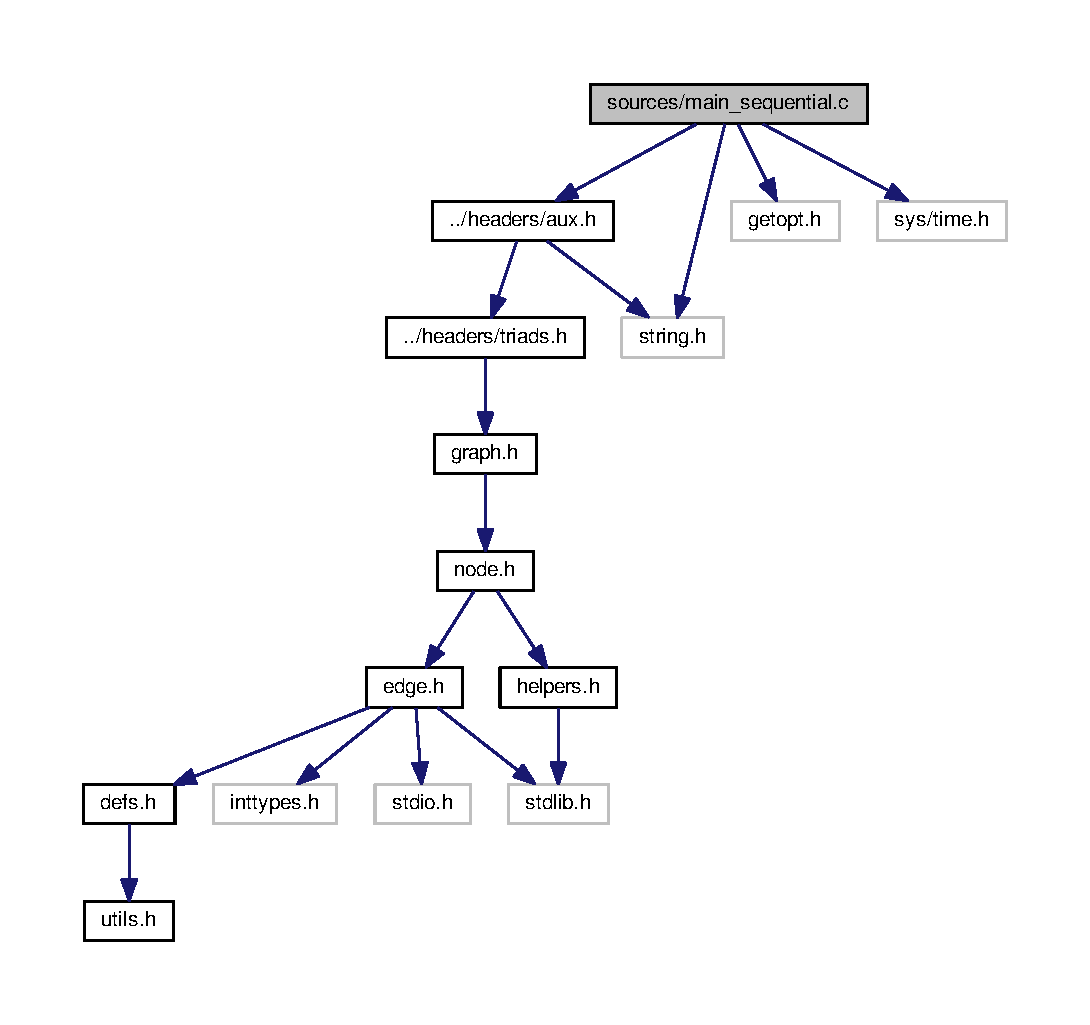
\includegraphics[width=350pt]{main__sequential_8c__incl}
\end{center}
\end{figure}
\subsection*{Macros}
\begin{DoxyCompactItemize}
\item 
\mbox{\Hypertarget{main__sequential_8c_a82acb32225c05e9aa4c524c40bc5852a}\label{main__sequential_8c_a82acb32225c05e9aa4c524c40bc5852a}} 
\#define {\bfseries M\+A\+X\+\_\+\+C\+H\+AR}~256
\item 
\mbox{\Hypertarget{main__sequential_8c_a485c7cb23461b12c0e1f62d795692738}\label{main__sequential_8c_a485c7cb23461b12c0e1f62d795692738}} 
\#define {\bfseries M\+A\+X\+\_\+\+F\+U\+NC}~5
\end{DoxyCompactItemize}
\subsection*{Functions}
\begin{DoxyCompactItemize}
\item 
\mbox{\Hypertarget{main__sequential_8c_a6d85d03371e68248c491c443a737c76f}\label{main__sequential_8c_a6d85d03371e68248c491c443a737c76f}} 
void {\bfseries display\+\_\+help} (char $\ast$program)
\item 
\mbox{\Hypertarget{main__sequential_8c_a3c04138a5bfe5d72780bb7e82a18e627}\label{main__sequential_8c_a3c04138a5bfe5d72780bb7e82a18e627}} 
int {\bfseries main} (int argc, char $\ast$$\ast$argv)
\end{DoxyCompactItemize}


\subsection{Detailed Description}
This is the main program of the sequential application. It executes a user-\/specified sequential version of triad census algorithm and displays results and execution performances depending on the parameters passed to the program. 

\begin{DoxyAuthor}{Author}
\+: Carlos Alfaro
\end{DoxyAuthor}
\begin{DoxyDate}{Date}
\+: 28-\/12-\/2017 
\end{DoxyDate}

\hypertarget{node_8c}{}\section{sources/node.c File Reference}
\label{node_8c}\index{sources/node.\+c@{sources/node.\+c}}


This file contains the code that implements the functions defined in the header file \hyperlink{node_8h}{node.\+h}. Please refer to it to check the documentation.  


{\ttfamily \#include \char`\"{}../headers/node.\+h\char`\"{}}\newline
Include dependency graph for node.\+c\+:
\nopagebreak
\begin{figure}[H]
\begin{center}
\leavevmode
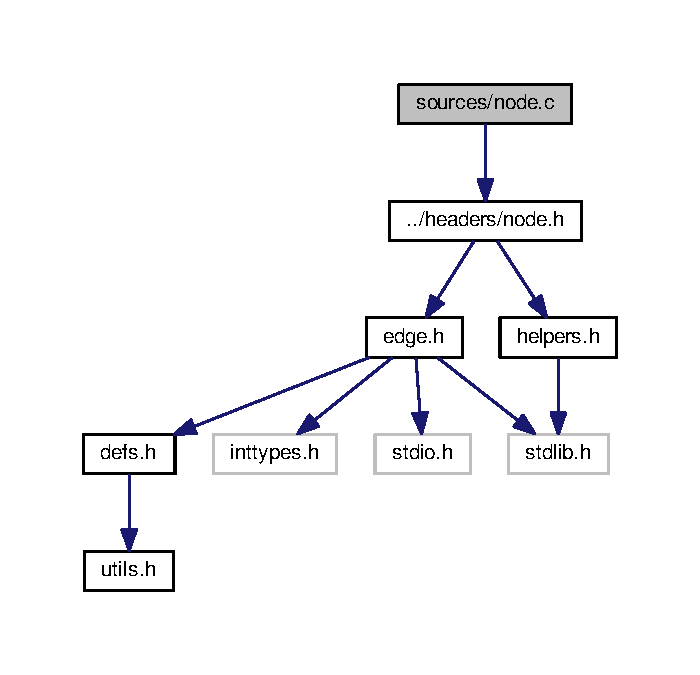
\includegraphics[width=336pt]{node_8c__incl}
\end{center}
\end{figure}
\subsection*{Functions}
\begin{DoxyCompactItemize}
\item 
\hyperlink{structNODE}{N\+O\+DE} $\ast$ \hyperlink{node_8c_a44b280e18f7f2ff59e126501cb5da4cf}{create\+\_\+node} (uint32\+\_\+t node\+\_\+id)
\begin{DoxyCompactList}\small\item\em Function that creates a new node, allocating memory for its fields and initializing them. The node\+\_\+id is set to the parameter passed, while the adj\+\_\+list is set to N\+U\+LL and the num\+\_\+neighbors is set to 0. \end{DoxyCompactList}\item 
\hyperlink{utils_8h_a32c27cc471df37f4fc818d65de0a56c4}{S\+T\+A\+T\+US} \hyperlink{node_8c_aacd383eaed2cba7aced7b1e032783f34}{add\+\_\+edge\+\_\+to\+\_\+node} (\hyperlink{structNODE}{N\+O\+DE} $\ast$node, uint32\+\_\+t neighbor\+\_\+id, \hyperlink{utils_8h_aa268a41a13430b18e933ed40207178d0}{D\+I\+R\+E\+C\+T\+I\+ON} dir)
\begin{DoxyCompactList}\small\item\em Function that creates a new node, allocating memory for its fields and initializing them. The node\+\_\+id is set to the parameter passed, while the adj\+\_\+list is set to N\+U\+LL and the num\+\_\+neighbors is set to 0. \end{DoxyCompactList}\item 
int \hyperlink{node_8c_a5b0769e751658fc3d9768c079ecba12c}{get\+\_\+neighbor\+\_\+pos} (\hyperlink{structNODE}{N\+O\+DE} $\ast$n, uint32\+\_\+t neighbor\+\_\+id)
\begin{DoxyCompactList}\small\item\em Function that returns the position of a certain neighbor node within the adjacency list of the node, given the neighbor id. \end{DoxyCompactList}\item 
\hyperlink{utils_8h_a3e5b8192e7d9ffaf3542f1210aec18dd}{B\+O\+OL} \hyperlink{node_8c_a37de73278d193b74aed6a86833cb8c87}{not\+\_\+connected} (\hyperlink{structNODE}{N\+O\+DE} $\ast$u, \hyperlink{structNODE}{N\+O\+DE} $\ast$v)
\begin{DoxyCompactList}\small\item\em Function that checks if two nodes u and v are connected. \end{DoxyCompactList}\item 
uint32\+\_\+t \hyperlink{node_8c_aed1bcaeca3d8358924632d6cf06dd29e}{get\+\_\+node\+\_\+id} (\hyperlink{structNODE}{N\+O\+DE} $\ast$n)
\begin{DoxyCompactList}\small\item\em Function that returns id of a certain node. \end{DoxyCompactList}\item 
\hyperlink{edge_8h_ab4a642fc78a44ca8df119570b3288e13}{E\+D\+GE} \hyperlink{node_8c_a1f56c95c3bf68181e75cef1e8a4ff2fc}{get\+\_\+edge} (\hyperlink{structNODE}{N\+O\+DE} $\ast$n, int pos)
\begin{DoxyCompactList}\small\item\em Function that the edge present in a certain position~\newline
of the adjacency list of a node. \end{DoxyCompactList}\item 
\hyperlink{edge_8h_ab4a642fc78a44ca8df119570b3288e13}{E\+D\+GE} $\ast$ \hyperlink{node_8c_a304e4f1cf8e0dbadd842ac4c8336c9f1}{get\+\_\+adj\+\_\+list} (\hyperlink{structNODE}{N\+O\+DE} $\ast$n)
\begin{DoxyCompactList}\small\item\em Function that returns the adjacency list of a certain node. \end{DoxyCompactList}\item 
int \hyperlink{node_8c_a02799b8fad8a4f676a9a6d5d0b82c366}{get\+\_\+num\+\_\+neighbors} (\hyperlink{structNODE}{N\+O\+DE} $\ast$n)
\begin{DoxyCompactList}\small\item\em Function that returns the number of neighbors a certain node has. \end{DoxyCompactList}\item 
int \hyperlink{node_8c_a6c59974e491a07d3c328570d42c3dbdb}{get\+\_\+degree} (\hyperlink{structNODE}{N\+O\+DE} $\ast$n)
\begin{DoxyCompactList}\small\item\em Function that returns the degree of a certain node. \end{DoxyCompactList}\item 
int \hyperlink{node_8c_aab41692fa3f3d5214a5dadb4f616a853}{comp\+\_\+nodes\+\_\+by\+\_\+id} (const void $\ast$key, const void $\ast$pnode)
\begin{DoxyCompactList}\small\item\em Function that compares two nodes (useful for binary search and insertion sort).~\newline
The comparison is made based on the node ids. \end{DoxyCompactList}\item 
int \hyperlink{node_8c_ac2c976ce0d52406c4df50195371276b8}{comp\+\_\+nodes\+\_\+by\+\_\+degree} (const void $\ast$key, const void $\ast$pnode)
\begin{DoxyCompactList}\small\item\em Function that compares two nodes (useful for binary search and insertion sort).~\newline
The comparison is made based on the number of neighbors of each node. \end{DoxyCompactList}\item 
int \hyperlink{node_8c_ab797719885a33013788cb2d4b248a36e}{comp\+\_\+ids} (const void $\ast$key, const void $\ast$pid)
\begin{DoxyCompactList}\small\item\em Function that compares two ids (useful for binary search and insertion sort). \end{DoxyCompactList}\item 
void \hyperlink{node_8c_abd4c035d081c773dff95d4f62a781ef6}{insert\+\_\+nodes} (void $\ast$nodes, void $\ast$node, int pos)
\begin{DoxyCompactList}\small\item\em Function that inserts a node in a list for nodes ~\newline
(useful for the helper function insert\+\_\+sort) \end{DoxyCompactList}\item 
uint32\+\_\+t $\ast$ \hyperlink{node_8c_af2840bd87ae7f23b8f0416f47ddb67da}{union\+\_\+adj\+\_\+lists\+\_\+ordered} (int $\ast$card\+\_\+S, \hyperlink{structNODE}{N\+O\+DE} $\ast$u, \hyperlink{structNODE}{N\+O\+DE} $\ast$v)
\begin{DoxyCompactList}\small\item\em Function that constructs the ordered union of the adjacency lists of two nodes ~\newline
 u and v, storing only the neighbor ids and avoiding the insertion of ~\newline
 u and v (in case they were present in the lists).~\newline
 The function also fills the parameter card\+\_\+S with the cardinality of the ~\newline
 union. \end{DoxyCompactList}\item 
uint32\+\_\+t $\ast$ \hyperlink{node_8c_a9bef0eea3e19f9545e070374f5abc055}{union\+\_\+adj\+\_\+lists\+\_\+not\+\_\+ordered} (int $\ast$card\+\_\+S, \hyperlink{structNODE}{N\+O\+DE} $\ast$u, \hyperlink{structNODE}{N\+O\+DE} $\ast$v)
\begin{DoxyCompactList}\small\item\em Function that constructs the not ordered union of the adjacency lists of two nodes ~\newline
 u and v, storing only the neighbor ids and avoiding the insertion of ~\newline
 u and v (in case they were present in the lists).~\newline
 The function also fills the parameter card\+\_\+S with the cardinality of the~\newline
 union. \end{DoxyCompactList}\item 
\hyperlink{utils_8h_aa268a41a13430b18e933ed40207178d0}{D\+I\+R\+E\+C\+T\+I\+ON} \hyperlink{node_8c_acfeda132522226efe0dcab8ff2813da3}{get\+\_\+dir\+\_\+between\+\_\+nodes} (\hyperlink{structNODE}{N\+O\+DE} $\ast$u, \hyperlink{structNODE}{N\+O\+DE} $\ast$v)
\begin{DoxyCompactList}\small\item\em Function that constructs the union of the adjacency lists of two nodes~\newline
 u and v, storing only the neighbor ids and avoiding the insertion of ~\newline
 u and v (in case they were present in the lists).~\newline
 The function also fills the parameter card\+\_\+S with the cardinality of the~\newline
 union. \end{DoxyCompactList}\item 
void \hyperlink{node_8c_ac537b7cd330634c71ec43a4ce258c3b1}{print\+\_\+node} (\hyperlink{structNODE}{N\+O\+DE} $\ast$n)
\begin{DoxyCompactList}\small\item\em Function that prints the information of a node. \end{DoxyCompactList}\item 
void \hyperlink{node_8c_a3f5e6b88f2394c03ffa21bd8e4bdb9c0}{destroy\+\_\+node} (\hyperlink{structNODE}{N\+O\+DE} $\ast$n)
\begin{DoxyCompactList}\small\item\em Function that destroys a node, freeing the memory of ~\newline
 its structures. \end{DoxyCompactList}\end{DoxyCompactItemize}
\subsection*{Variables}
\begin{DoxyCompactItemize}
\item 
\hyperlink{utils_8h_a3e5b8192e7d9ffaf3542f1210aec18dd}{B\+O\+OL} \hyperlink{node_8c_aa94b0ac5dc0f8919227cda71fe50db38}{ordered}
\end{DoxyCompactItemize}


\subsection{Detailed Description}
This file contains the code that implements the functions defined in the header file \hyperlink{node_8h}{node.\+h}. Please refer to it to check the documentation. 

\begin{DoxyAuthor}{Author}
\+: Carlos Alfaro
\end{DoxyAuthor}
\begin{DoxyDate}{Date}
\+: 23-\/10-\/2017 
\end{DoxyDate}


\subsection{Function Documentation}
\mbox{\Hypertarget{node_8c_aacd383eaed2cba7aced7b1e032783f34}\label{node_8c_aacd383eaed2cba7aced7b1e032783f34}} 
\index{node.\+c@{node.\+c}!add\+\_\+edge\+\_\+to\+\_\+node@{add\+\_\+edge\+\_\+to\+\_\+node}}
\index{add\+\_\+edge\+\_\+to\+\_\+node@{add\+\_\+edge\+\_\+to\+\_\+node}!node.\+c@{node.\+c}}
\subsubsection{\texorpdfstring{add\+\_\+edge\+\_\+to\+\_\+node()}{add\_edge\_to\_node()}}
{\footnotesize\ttfamily \hyperlink{utils_8h_a32c27cc471df37f4fc818d65de0a56c4}{S\+T\+A\+T\+US} add\+\_\+edge\+\_\+to\+\_\+node (\begin{DoxyParamCaption}\item[{\hyperlink{structNODE}{N\+O\+DE} $\ast$}]{n,  }\item[{uint32\+\_\+t}]{neighbor\+\_\+id,  }\item[{\hyperlink{utils_8h_aa268a41a13430b18e933ed40207178d0}{D\+I\+R\+E\+C\+T\+I\+ON}}]{dir }\end{DoxyParamCaption})}



Function that creates a new node, allocating memory for its fields and initializing them. The node\+\_\+id is set to the parameter passed, while the adj\+\_\+list is set to N\+U\+LL and the num\+\_\+neighbors is set to 0. 


\begin{DoxyParams}{Parameters}
{\em N\+O\+D\+E$\ast$} & n\+: The node in which we want to insert the edge \\
\hline
{\em uint32\+\_\+t} & neighbor\+\_\+id\+: The node id of the neighbor we want to insert \\
\hline
{\em D\+I\+R\+E\+C\+T\+I\+ON} & dir\+: The direction of the edge we want to insert\\
\hline
\end{DoxyParams}
\begin{DoxyReturn}{Returns}
S\+T\+A\+T\+US\+: OK if the insertion was successful E\+RR otherwise 
\end{DoxyReturn}
\mbox{\Hypertarget{node_8c_ab797719885a33013788cb2d4b248a36e}\label{node_8c_ab797719885a33013788cb2d4b248a36e}} 
\index{node.\+c@{node.\+c}!comp\+\_\+ids@{comp\+\_\+ids}}
\index{comp\+\_\+ids@{comp\+\_\+ids}!node.\+c@{node.\+c}}
\subsubsection{\texorpdfstring{comp\+\_\+ids()}{comp\_ids()}}
{\footnotesize\ttfamily int comp\+\_\+ids (\begin{DoxyParamCaption}\item[{const void $\ast$}]{key,  }\item[{const void $\ast$}]{pid }\end{DoxyParamCaption})}



Function that compares two ids (useful for binary search and insertion sort). 


\begin{DoxyParams}{Parameters}
{\em const} & void$\ast$ key\+: The key we want to compare to the pointer. It is a pointer an id. \\
\hline
{\em const} & void$\ast$ pid\+: A pointer to the id we want to compare to the key\\
\hline
\end{DoxyParams}
\begin{DoxyReturn}{Returns}
int A number that is less than, greater than or equal to 0, depending on weather the key is less than, greather than or equal to the id. 
\end{DoxyReturn}
\mbox{\Hypertarget{node_8c_ac2c976ce0d52406c4df50195371276b8}\label{node_8c_ac2c976ce0d52406c4df50195371276b8}} 
\index{node.\+c@{node.\+c}!comp\+\_\+nodes\+\_\+by\+\_\+degree@{comp\+\_\+nodes\+\_\+by\+\_\+degree}}
\index{comp\+\_\+nodes\+\_\+by\+\_\+degree@{comp\+\_\+nodes\+\_\+by\+\_\+degree}!node.\+c@{node.\+c}}
\subsubsection{\texorpdfstring{comp\+\_\+nodes\+\_\+by\+\_\+degree()}{comp\_nodes\_by\_degree()}}
{\footnotesize\ttfamily int comp\+\_\+nodes\+\_\+by\+\_\+degree (\begin{DoxyParamCaption}\item[{const void $\ast$}]{key,  }\item[{const void $\ast$}]{pnode }\end{DoxyParamCaption})}



Function that compares two nodes (useful for binary search and insertion sort).~\newline
The comparison is made based on the number of neighbors of each node. 


\begin{DoxyParams}{Parameters}
{\em const} & void$\ast$ key\+: The key we want to compare to the other node. It is a pointer to the number of neighbors of a node. \\
\hline
{\em const} & void$\ast$ pnode\+: A pointer to the node we want to compare to the key\\
\hline
\end{DoxyParams}
\begin{DoxyReturn}{Returns}
int A number that is less than, greater than or equal to 0, depending on weather the key is less than, greather than or equal to the pnode. 
\end{DoxyReturn}
\mbox{\Hypertarget{node_8c_aab41692fa3f3d5214a5dadb4f616a853}\label{node_8c_aab41692fa3f3d5214a5dadb4f616a853}} 
\index{node.\+c@{node.\+c}!comp\+\_\+nodes\+\_\+by\+\_\+id@{comp\+\_\+nodes\+\_\+by\+\_\+id}}
\index{comp\+\_\+nodes\+\_\+by\+\_\+id@{comp\+\_\+nodes\+\_\+by\+\_\+id}!node.\+c@{node.\+c}}
\subsubsection{\texorpdfstring{comp\+\_\+nodes\+\_\+by\+\_\+id()}{comp\_nodes\_by\_id()}}
{\footnotesize\ttfamily int comp\+\_\+nodes\+\_\+by\+\_\+id (\begin{DoxyParamCaption}\item[{const void $\ast$}]{key,  }\item[{const void $\ast$}]{pnode }\end{DoxyParamCaption})}



Function that compares two nodes (useful for binary search and insertion sort).~\newline
The comparison is made based on the node ids. 


\begin{DoxyParams}{Parameters}
{\em const} & void$\ast$ key\+: The key we want to compare to the other node. It is a pointer to a node id. \\
\hline
{\em const} & void$\ast$ pnode\+: A pointer to the node we want to compare to the key\\
\hline
\end{DoxyParams}
\begin{DoxyReturn}{Returns}
int A number that is less than, greater than or equal to 0, depending on weather the key is less than, greather than or equal to the pnode. 
\end{DoxyReturn}
\mbox{\Hypertarget{node_8c_a44b280e18f7f2ff59e126501cb5da4cf}\label{node_8c_a44b280e18f7f2ff59e126501cb5da4cf}} 
\index{node.\+c@{node.\+c}!create\+\_\+node@{create\+\_\+node}}
\index{create\+\_\+node@{create\+\_\+node}!node.\+c@{node.\+c}}
\subsubsection{\texorpdfstring{create\+\_\+node()}{create\_node()}}
{\footnotesize\ttfamily \hyperlink{structNODE}{N\+O\+DE}$\ast$ create\+\_\+node (\begin{DoxyParamCaption}\item[{uint32\+\_\+t}]{node\+\_\+id }\end{DoxyParamCaption})}



Function that creates a new node, allocating memory for its fields and initializing them. The node\+\_\+id is set to the parameter passed, while the adj\+\_\+list is set to N\+U\+LL and the num\+\_\+neighbors is set to 0. 


\begin{DoxyParams}{Parameters}
{\em uint32\+\_\+t} & node\+\_\+id\+: The id of the node\\
\hline
\end{DoxyParams}
\begin{DoxyReturn}{Returns}
N\+O\+D\+E$\ast$\+: A pointer to the node just created. 
\end{DoxyReturn}
\mbox{\Hypertarget{node_8c_a3f5e6b88f2394c03ffa21bd8e4bdb9c0}\label{node_8c_a3f5e6b88f2394c03ffa21bd8e4bdb9c0}} 
\index{node.\+c@{node.\+c}!destroy\+\_\+node@{destroy\+\_\+node}}
\index{destroy\+\_\+node@{destroy\+\_\+node}!node.\+c@{node.\+c}}
\subsubsection{\texorpdfstring{destroy\+\_\+node()}{destroy\_node()}}
{\footnotesize\ttfamily void destroy\+\_\+node (\begin{DoxyParamCaption}\item[{\hyperlink{structNODE}{N\+O\+DE} $\ast$}]{n }\end{DoxyParamCaption})}



Function that destroys a node, freeing the memory of ~\newline
 its structures. 


\begin{DoxyParams}{Parameters}
{\em N\+O\+D\+E$\ast$} & n\+: the node to destroy\\
\hline
\end{DoxyParams}
\begin{DoxyReturn}{Returns}
none 
\end{DoxyReturn}
\mbox{\Hypertarget{node_8c_a304e4f1cf8e0dbadd842ac4c8336c9f1}\label{node_8c_a304e4f1cf8e0dbadd842ac4c8336c9f1}} 
\index{node.\+c@{node.\+c}!get\+\_\+adj\+\_\+list@{get\+\_\+adj\+\_\+list}}
\index{get\+\_\+adj\+\_\+list@{get\+\_\+adj\+\_\+list}!node.\+c@{node.\+c}}
\subsubsection{\texorpdfstring{get\+\_\+adj\+\_\+list()}{get\_adj\_list()}}
{\footnotesize\ttfamily \hyperlink{edge_8h_ab4a642fc78a44ca8df119570b3288e13}{E\+D\+GE}$\ast$ get\+\_\+adj\+\_\+list (\begin{DoxyParamCaption}\item[{\hyperlink{structNODE}{N\+O\+DE} $\ast$}]{n }\end{DoxyParamCaption})}



Function that returns the adjacency list of a certain node. 


\begin{DoxyParams}{Parameters}
{\em N\+O\+D\+E$\ast$} & n\+: The node of which we want to get the adjacency list\\
\hline
\end{DoxyParams}
\begin{DoxyReturn}{Returns}
E\+D\+G\+E$\ast$\+: The adjacency list 
\end{DoxyReturn}
\mbox{\Hypertarget{node_8c_a6c59974e491a07d3c328570d42c3dbdb}\label{node_8c_a6c59974e491a07d3c328570d42c3dbdb}} 
\index{node.\+c@{node.\+c}!get\+\_\+degree@{get\+\_\+degree}}
\index{get\+\_\+degree@{get\+\_\+degree}!node.\+c@{node.\+c}}
\subsubsection{\texorpdfstring{get\+\_\+degree()}{get\_degree()}}
{\footnotesize\ttfamily int get\+\_\+degree (\begin{DoxyParamCaption}\item[{\hyperlink{structNODE}{N\+O\+DE} $\ast$}]{n }\end{DoxyParamCaption})}



Function that returns the degree of a certain node. 


\begin{DoxyParams}{Parameters}
{\em N\+O\+D\+E$\ast$} & n\+: The node of which we want to discover the degree\\
\hline
\end{DoxyParams}
\begin{DoxyReturn}{Returns}
int the degree 
\end{DoxyReturn}
\mbox{\Hypertarget{node_8c_acfeda132522226efe0dcab8ff2813da3}\label{node_8c_acfeda132522226efe0dcab8ff2813da3}} 
\index{node.\+c@{node.\+c}!get\+\_\+dir\+\_\+between\+\_\+nodes@{get\+\_\+dir\+\_\+between\+\_\+nodes}}
\index{get\+\_\+dir\+\_\+between\+\_\+nodes@{get\+\_\+dir\+\_\+between\+\_\+nodes}!node.\+c@{node.\+c}}
\subsubsection{\texorpdfstring{get\+\_\+dir\+\_\+between\+\_\+nodes()}{get\_dir\_between\_nodes()}}
{\footnotesize\ttfamily \hyperlink{utils_8h_aa268a41a13430b18e933ed40207178d0}{D\+I\+R\+E\+C\+T\+I\+ON} get\+\_\+dir\+\_\+between\+\_\+nodes (\begin{DoxyParamCaption}\item[{\hyperlink{structNODE}{N\+O\+DE} $\ast$}]{u,  }\item[{\hyperlink{structNODE}{N\+O\+DE} $\ast$}]{v }\end{DoxyParamCaption})}



Function that constructs the union of the adjacency lists of two nodes~\newline
 u and v, storing only the neighbor ids and avoiding the insertion of ~\newline
 u and v (in case they were present in the lists).~\newline
 The function also fills the parameter card\+\_\+S with the cardinality of the~\newline
 union. 


\begin{DoxyParams}{Parameters}
{\em N\+O\+D\+E$\ast$} & u\+: The first node \\
\hline
{\em N\+O\+D\+E$\ast$} & v\+: The second node\\
\hline
\end{DoxyParams}
\begin{DoxyReturn}{Returns}
D\+I\+R\+E\+C\+T\+I\+ON\+: The direction between the two nodes\+:~\newline
 I\+N\+\_\+\+O\+UT, O\+U\+T\+\_\+\+IN, or B\+I\+D\+I\+R\+E\+C\+T\+I\+O\+N\+AL in case they are connected.~\newline
 N\+O\+NE in case they are not connected 
\end{DoxyReturn}
\mbox{\Hypertarget{node_8c_a1f56c95c3bf68181e75cef1e8a4ff2fc}\label{node_8c_a1f56c95c3bf68181e75cef1e8a4ff2fc}} 
\index{node.\+c@{node.\+c}!get\+\_\+edge@{get\+\_\+edge}}
\index{get\+\_\+edge@{get\+\_\+edge}!node.\+c@{node.\+c}}
\subsubsection{\texorpdfstring{get\+\_\+edge()}{get\_edge()}}
{\footnotesize\ttfamily \hyperlink{edge_8h_ab4a642fc78a44ca8df119570b3288e13}{E\+D\+GE} get\+\_\+edge (\begin{DoxyParamCaption}\item[{\hyperlink{structNODE}{N\+O\+DE} $\ast$}]{n,  }\item[{int}]{pos }\end{DoxyParamCaption})}



Function that the edge present in a certain position~\newline
of the adjacency list of a node. 


\begin{DoxyParams}{Parameters}
{\em N\+O\+D\+E$\ast$} & n\+: The node from which we want to get the edge \\
\hline
{\em int} & pos\+: The position within the adjacency list\\
\hline
\end{DoxyParams}
\begin{DoxyReturn}{Returns}
E\+D\+GE\+: the edge 
\end{DoxyReturn}
\mbox{\Hypertarget{node_8c_a5b0769e751658fc3d9768c079ecba12c}\label{node_8c_a5b0769e751658fc3d9768c079ecba12c}} 
\index{node.\+c@{node.\+c}!get\+\_\+neighbor\+\_\+pos@{get\+\_\+neighbor\+\_\+pos}}
\index{get\+\_\+neighbor\+\_\+pos@{get\+\_\+neighbor\+\_\+pos}!node.\+c@{node.\+c}}
\subsubsection{\texorpdfstring{get\+\_\+neighbor\+\_\+pos()}{get\_neighbor\_pos()}}
{\footnotesize\ttfamily int get\+\_\+neighbor\+\_\+pos (\begin{DoxyParamCaption}\item[{\hyperlink{structNODE}{N\+O\+DE} $\ast$}]{n,  }\item[{uint32\+\_\+t}]{neighbor\+\_\+id }\end{DoxyParamCaption})}



Function that returns the position of a certain neighbor node within the adjacency list of the node, given the neighbor id. 

Getter functions 
\begin{DoxyParams}{Parameters}
{\em N\+O\+D\+E$\ast$} & n\+: The node of which we want to get the neighbor position \\
\hline
{\em uint32\+\_\+t} & neighbor\+\_\+id\+: The node id of the neighbor we want to search\\
\hline
\end{DoxyParams}
\begin{DoxyReturn}{Returns}
int\+: The position within the adjacency list 
\end{DoxyReturn}
\mbox{\Hypertarget{node_8c_aed1bcaeca3d8358924632d6cf06dd29e}\label{node_8c_aed1bcaeca3d8358924632d6cf06dd29e}} 
\index{node.\+c@{node.\+c}!get\+\_\+node\+\_\+id@{get\+\_\+node\+\_\+id}}
\index{get\+\_\+node\+\_\+id@{get\+\_\+node\+\_\+id}!node.\+c@{node.\+c}}
\subsubsection{\texorpdfstring{get\+\_\+node\+\_\+id()}{get\_node\_id()}}
{\footnotesize\ttfamily uint32\+\_\+t get\+\_\+node\+\_\+id (\begin{DoxyParamCaption}\item[{\hyperlink{structNODE}{N\+O\+DE} $\ast$}]{n }\end{DoxyParamCaption})}



Function that returns id of a certain node. 


\begin{DoxyParams}{Parameters}
{\em N\+O\+D\+E$\ast$} & n\+: The node of which we want to discover the id\\
\hline
\end{DoxyParams}
\begin{DoxyReturn}{Returns}
uint32\+\_\+t\+: the node id 
\end{DoxyReturn}
\mbox{\Hypertarget{node_8c_a02799b8fad8a4f676a9a6d5d0b82c366}\label{node_8c_a02799b8fad8a4f676a9a6d5d0b82c366}} 
\index{node.\+c@{node.\+c}!get\+\_\+num\+\_\+neighbors@{get\+\_\+num\+\_\+neighbors}}
\index{get\+\_\+num\+\_\+neighbors@{get\+\_\+num\+\_\+neighbors}!node.\+c@{node.\+c}}
\subsubsection{\texorpdfstring{get\+\_\+num\+\_\+neighbors()}{get\_num\_neighbors()}}
{\footnotesize\ttfamily int get\+\_\+num\+\_\+neighbors (\begin{DoxyParamCaption}\item[{\hyperlink{structNODE}{N\+O\+DE} $\ast$}]{n }\end{DoxyParamCaption})}



Function that returns the number of neighbors a certain node has. 


\begin{DoxyParams}{Parameters}
{\em N\+O\+D\+E$\ast$} & n\+: The node of which we want to discover the number of neighbors\\
\hline
\end{DoxyParams}
\begin{DoxyReturn}{Returns}
int the number of neighbors 
\end{DoxyReturn}
\mbox{\Hypertarget{node_8c_abd4c035d081c773dff95d4f62a781ef6}\label{node_8c_abd4c035d081c773dff95d4f62a781ef6}} 
\index{node.\+c@{node.\+c}!insert\+\_\+nodes@{insert\+\_\+nodes}}
\index{insert\+\_\+nodes@{insert\+\_\+nodes}!node.\+c@{node.\+c}}
\subsubsection{\texorpdfstring{insert\+\_\+nodes()}{insert\_nodes()}}
{\footnotesize\ttfamily void insert\+\_\+nodes (\begin{DoxyParamCaption}\item[{void $\ast$}]{nodes,  }\item[{void $\ast$}]{node,  }\item[{int}]{pos }\end{DoxyParamCaption})}



Function that inserts a node in a list for nodes ~\newline
(useful for the helper function insert\+\_\+sort) 


\begin{DoxyParams}{Parameters}
{\em void$\ast$} & nodes\+: The list of nodes in which we want to insert the new node \\
\hline
{\em const} & void$\ast$ node\+: The node to insert \\
\hline
{\em int} & pos\+: The position in which to insert\\
\hline
\end{DoxyParams}
\begin{DoxyReturn}{Returns}
None 
\end{DoxyReturn}
\mbox{\Hypertarget{node_8c_a37de73278d193b74aed6a86833cb8c87}\label{node_8c_a37de73278d193b74aed6a86833cb8c87}} 
\index{node.\+c@{node.\+c}!not\+\_\+connected@{not\+\_\+connected}}
\index{not\+\_\+connected@{not\+\_\+connected}!node.\+c@{node.\+c}}
\subsubsection{\texorpdfstring{not\+\_\+connected()}{not\_connected()}}
{\footnotesize\ttfamily \hyperlink{utils_8h_a3e5b8192e7d9ffaf3542f1210aec18dd}{B\+O\+OL} not\+\_\+connected (\begin{DoxyParamCaption}\item[{\hyperlink{structNODE}{N\+O\+DE} $\ast$}]{u,  }\item[{\hyperlink{structNODE}{N\+O\+DE} $\ast$}]{v }\end{DoxyParamCaption})}



Function that checks if two nodes u and v are connected. 


\begin{DoxyParams}{Parameters}
{\em N\+O\+D\+E$\ast$} & u\+: The first node \\
\hline
{\em N\+O\+D\+E$\ast$} & v\+: The second node\\
\hline
\end{DoxyParams}
\begin{DoxyReturn}{Returns}
B\+O\+OL T\+R\+UE if the nodes u and v are not connected.~\newline
 F\+A\+L\+SE if u and v are connected. 
\end{DoxyReturn}
\mbox{\Hypertarget{node_8c_ac537b7cd330634c71ec43a4ce258c3b1}\label{node_8c_ac537b7cd330634c71ec43a4ce258c3b1}} 
\index{node.\+c@{node.\+c}!print\+\_\+node@{print\+\_\+node}}
\index{print\+\_\+node@{print\+\_\+node}!node.\+c@{node.\+c}}
\subsubsection{\texorpdfstring{print\+\_\+node()}{print\_node()}}
{\footnotesize\ttfamily void print\+\_\+node (\begin{DoxyParamCaption}\item[{\hyperlink{structNODE}{N\+O\+DE} $\ast$}]{n }\end{DoxyParamCaption})}



Function that prints the information of a node. 


\begin{DoxyParams}{Parameters}
{\em N\+O\+D\+E$\ast$} & n\+: the node to print\\
\hline
\end{DoxyParams}
\begin{DoxyReturn}{Returns}
none 
\end{DoxyReturn}
\mbox{\Hypertarget{node_8c_a9bef0eea3e19f9545e070374f5abc055}\label{node_8c_a9bef0eea3e19f9545e070374f5abc055}} 
\index{node.\+c@{node.\+c}!union\+\_\+adj\+\_\+lists\+\_\+not\+\_\+ordered@{union\+\_\+adj\+\_\+lists\+\_\+not\+\_\+ordered}}
\index{union\+\_\+adj\+\_\+lists\+\_\+not\+\_\+ordered@{union\+\_\+adj\+\_\+lists\+\_\+not\+\_\+ordered}!node.\+c@{node.\+c}}
\subsubsection{\texorpdfstring{union\+\_\+adj\+\_\+lists\+\_\+not\+\_\+ordered()}{union\_adj\_lists\_not\_ordered()}}
{\footnotesize\ttfamily uint32\+\_\+t$\ast$ union\+\_\+adj\+\_\+lists\+\_\+not\+\_\+ordered (\begin{DoxyParamCaption}\item[{int $\ast$}]{card\+\_\+S,  }\item[{\hyperlink{structNODE}{N\+O\+DE} $\ast$}]{u,  }\item[{\hyperlink{structNODE}{N\+O\+DE} $\ast$}]{v }\end{DoxyParamCaption})}



Function that constructs the not ordered union of the adjacency lists of two nodes ~\newline
 u and v, storing only the neighbor ids and avoiding the insertion of ~\newline
 u and v (in case they were present in the lists).~\newline
 The function also fills the parameter card\+\_\+S with the cardinality of the~\newline
 union. 


\begin{DoxyParams}{Parameters}
{\em int$\ast$} & card\+\_\+S\+: The cardinality of the union (to be filled by the function) \\
\hline
{\em N\+O\+D\+E$\ast$} & u\+: The first node \\
\hline
{\em N\+O\+D\+E$\ast$} & v\+: The second node\\
\hline
\end{DoxyParams}
\begin{DoxyReturn}{Returns}
uint32\+\_\+t$\ast$ The array containing the node ids of the union. 
\end{DoxyReturn}
\mbox{\Hypertarget{node_8c_af2840bd87ae7f23b8f0416f47ddb67da}\label{node_8c_af2840bd87ae7f23b8f0416f47ddb67da}} 
\index{node.\+c@{node.\+c}!union\+\_\+adj\+\_\+lists\+\_\+ordered@{union\+\_\+adj\+\_\+lists\+\_\+ordered}}
\index{union\+\_\+adj\+\_\+lists\+\_\+ordered@{union\+\_\+adj\+\_\+lists\+\_\+ordered}!node.\+c@{node.\+c}}
\subsubsection{\texorpdfstring{union\+\_\+adj\+\_\+lists\+\_\+ordered()}{union\_adj\_lists\_ordered()}}
{\footnotesize\ttfamily uint32\+\_\+t$\ast$ union\+\_\+adj\+\_\+lists\+\_\+ordered (\begin{DoxyParamCaption}\item[{int $\ast$}]{card\+\_\+S,  }\item[{\hyperlink{structNODE}{N\+O\+DE} $\ast$}]{u,  }\item[{\hyperlink{structNODE}{N\+O\+DE} $\ast$}]{v }\end{DoxyParamCaption})}



Function that constructs the ordered union of the adjacency lists of two nodes ~\newline
 u and v, storing only the neighbor ids and avoiding the insertion of ~\newline
 u and v (in case they were present in the lists).~\newline
 The function also fills the parameter card\+\_\+S with the cardinality of the ~\newline
 union. 


\begin{DoxyParams}{Parameters}
{\em int$\ast$} & card\+\_\+S\+: The cardinality of the union (to be filled by the function) \\
\hline
{\em N\+O\+D\+E$\ast$} & u\+: The first node \\
\hline
{\em N\+O\+D\+E$\ast$} & v\+: The second node\\
\hline
\end{DoxyParams}
\begin{DoxyReturn}{Returns}
uint32\+\_\+t$\ast$ The array containing the node ids of the union. 
\end{DoxyReturn}


\subsection{Variable Documentation}
\mbox{\Hypertarget{node_8c_aa94b0ac5dc0f8919227cda71fe50db38}\label{node_8c_aa94b0ac5dc0f8919227cda71fe50db38}} 
\index{node.\+c@{node.\+c}!ordered@{ordered}}
\index{ordered@{ordered}!node.\+c@{node.\+c}}
\subsubsection{\texorpdfstring{ordered}{ordered}}
{\footnotesize\ttfamily \hyperlink{utils_8h_a3e5b8192e7d9ffaf3542f1210aec18dd}{B\+O\+OL} ordered}

Flag to determine whether the data managed has to be ordered or not 
\hypertarget{rand__graph__generation_8c}{}\section{sources/rand\+\_\+graph\+\_\+generation.c File Reference}
\label{rand__graph__generation_8c}\index{sources/rand\+\_\+graph\+\_\+generation.\+c@{sources/rand\+\_\+graph\+\_\+generation.\+c}}


This program generates a pseudo-\/random graph of a given number of nodes and edges and writes it to a file.  


{\ttfamily \#include $<$stdio.\+h$>$}\newline
{\ttfamily \#include $<$stdlib.\+h$>$}\newline
Include dependency graph for rand\+\_\+graph\+\_\+generation.\+c\+:
\nopagebreak
\begin{figure}[H]
\begin{center}
\leavevmode
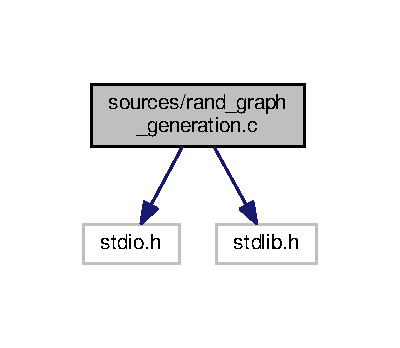
\includegraphics[width=192pt]{rand__graph__generation_8c__incl}
\end{center}
\end{figure}
\subsection*{Functions}
\begin{DoxyCompactItemize}
\item 
\mbox{\Hypertarget{rand__graph__generation_8c_a3c04138a5bfe5d72780bb7e82a18e627}\label{rand__graph__generation_8c_a3c04138a5bfe5d72780bb7e82a18e627}} 
int {\bfseries main} (int argc, char $\ast$$\ast$argv)
\end{DoxyCompactItemize}


\subsection{Detailed Description}
This program generates a pseudo-\/random graph of a given number of nodes and edges and writes it to a file. 

\begin{DoxyAuthor}{Author}
\+: Carlos Alfaro
\end{DoxyAuthor}
\begin{DoxyDate}{Date}
\+: 28-\/12-\/2017 
\end{DoxyDate}

\hypertarget{times__parallel_8c}{}\section{sources/times\+\_\+parallel.c File Reference}
\label{times__parallel_8c}\index{sources/times\+\_\+parallel.\+c@{sources/times\+\_\+parallel.\+c}}


This program collects execution performances of a user-\/specified accelerated version of the triad census algorithm and writes them to a file.  


{\ttfamily \#include \char`\"{}../headers/aux\+\_\+opencl.\+h\char`\"{}}\newline
{\ttfamily \#include $<$getopt.\+h$>$}\newline
{\ttfamily \#include $<$sys/time.\+h$>$}\newline
Include dependency graph for times\+\_\+parallel.\+c\+:
\nopagebreak
\begin{figure}[H]
\begin{center}
\leavevmode
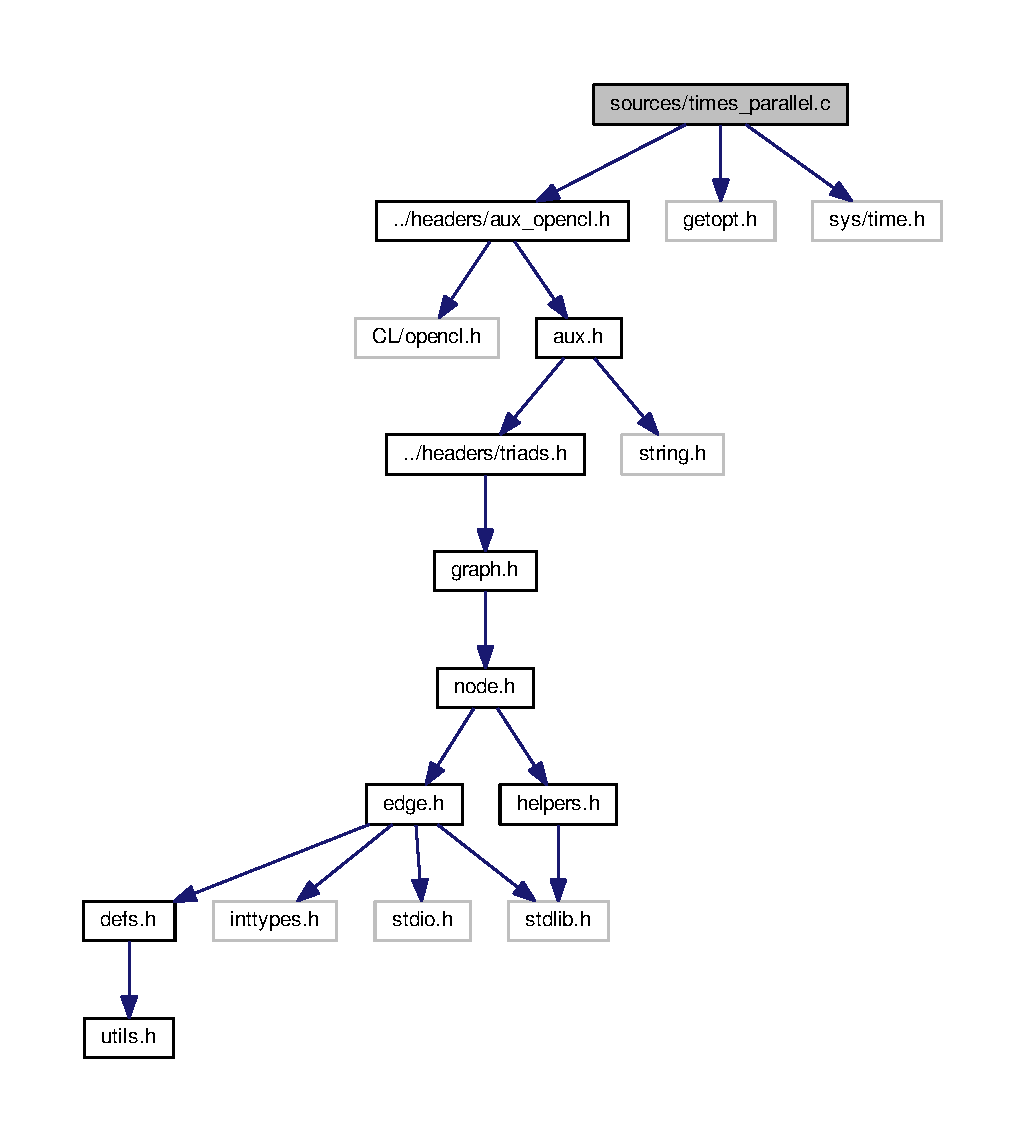
\includegraphics[width=350pt]{times__parallel_8c__incl}
\end{center}
\end{figure}
\subsection*{Functions}
\begin{DoxyCompactItemize}
\item 
\mbox{\Hypertarget{times__parallel_8c_a6d85d03371e68248c491c443a737c76f}\label{times__parallel_8c_a6d85d03371e68248c491c443a737c76f}} 
void {\bfseries display\+\_\+help} (char $\ast$program)
\item 
\mbox{\Hypertarget{times__parallel_8c_a3c04138a5bfe5d72780bb7e82a18e627}\label{times__parallel_8c_a3c04138a5bfe5d72780bb7e82a18e627}} 
int {\bfseries main} (int argc, char $\ast$$\ast$argv)
\end{DoxyCompactItemize}


\subsection{Detailed Description}
This program collects execution performances of a user-\/specified accelerated version of the triad census algorithm and writes them to a file. 

\begin{DoxyAuthor}{Author}
\+: Carlos Alfaro
\end{DoxyAuthor}
\begin{DoxyDate}{Date}
\+: 28-\/12-\/2017 
\end{DoxyDate}

\hypertarget{times__sequential_8c}{}\section{sources/times\+\_\+sequential.c File Reference}
\label{times__sequential_8c}\index{sources/times\+\_\+sequential.\+c@{sources/times\+\_\+sequential.\+c}}


This program collects execution performances of a user-\/specified sequential version of the triad census algorithm and writes them to a file.  


{\ttfamily \#include \char`\"{}../headers/aux.\+h\char`\"{}}\newline
{\ttfamily \#include $<$string.\+h$>$}\newline
{\ttfamily \#include $<$getopt.\+h$>$}\newline
{\ttfamily \#include $<$sys/time.\+h$>$}\newline
Include dependency graph for times\+\_\+sequential.\+c\+:
\nopagebreak
\begin{figure}[H]
\begin{center}
\leavevmode
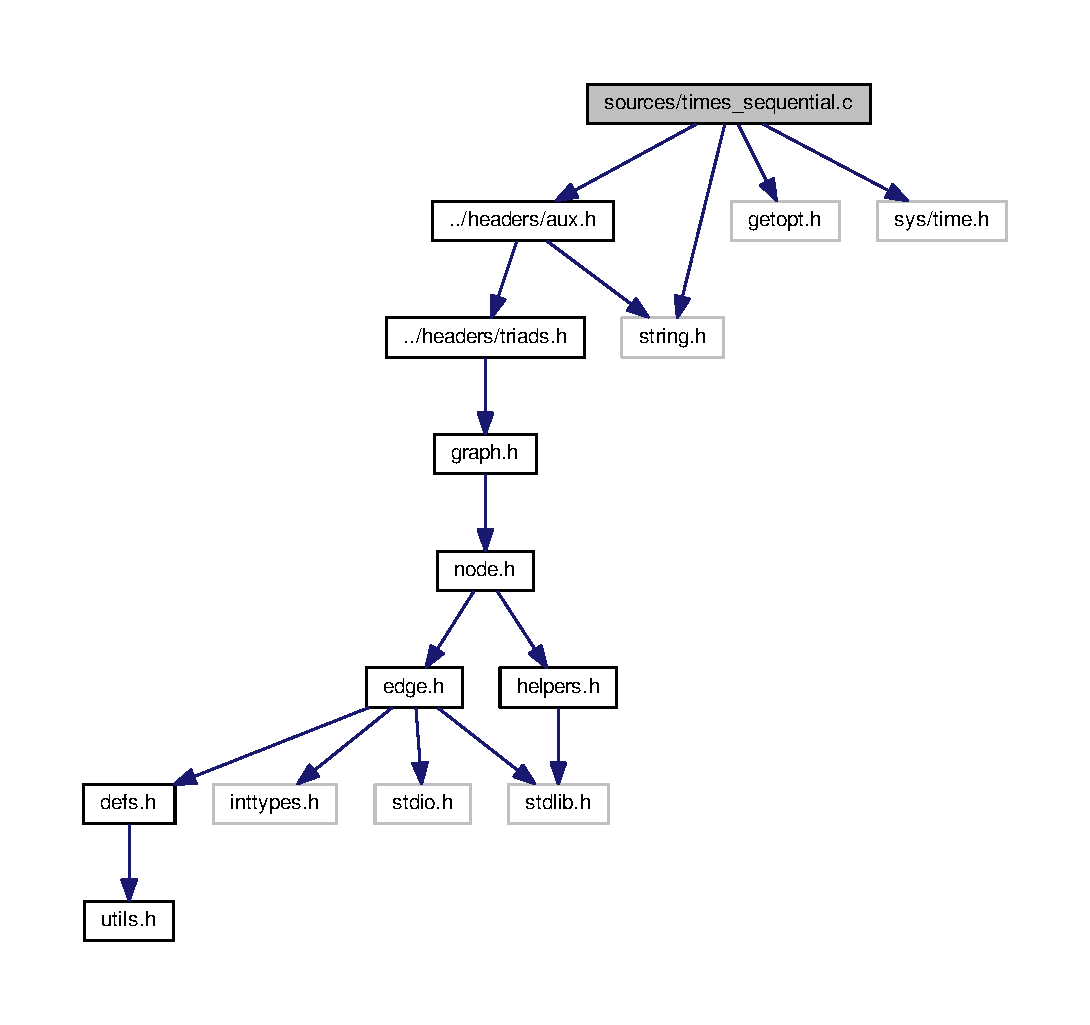
\includegraphics[width=350pt]{times__sequential_8c__incl}
\end{center}
\end{figure}
\subsection*{Macros}
\begin{DoxyCompactItemize}
\item 
\mbox{\Hypertarget{times__sequential_8c_a82acb32225c05e9aa4c524c40bc5852a}\label{times__sequential_8c_a82acb32225c05e9aa4c524c40bc5852a}} 
\#define {\bfseries M\+A\+X\+\_\+\+C\+H\+AR}~256
\item 
\mbox{\Hypertarget{times__sequential_8c_a485c7cb23461b12c0e1f62d795692738}\label{times__sequential_8c_a485c7cb23461b12c0e1f62d795692738}} 
\#define {\bfseries M\+A\+X\+\_\+\+F\+U\+NC}~5
\end{DoxyCompactItemize}
\subsection*{Functions}
\begin{DoxyCompactItemize}
\item 
\mbox{\Hypertarget{times__sequential_8c_a6d85d03371e68248c491c443a737c76f}\label{times__sequential_8c_a6d85d03371e68248c491c443a737c76f}} 
void {\bfseries display\+\_\+help} (char $\ast$program)
\item 
\mbox{\Hypertarget{times__sequential_8c_a3c04138a5bfe5d72780bb7e82a18e627}\label{times__sequential_8c_a3c04138a5bfe5d72780bb7e82a18e627}} 
int {\bfseries main} (int argc, char $\ast$$\ast$argv)
\end{DoxyCompactItemize}


\subsection{Detailed Description}
This program collects execution performances of a user-\/specified sequential version of the triad census algorithm and writes them to a file. 

\begin{DoxyAuthor}{Author}
\+: Carlos Alfaro
\end{DoxyAuthor}
\begin{DoxyDate}{Date}
\+: 28-\/12-\/2017 
\end{DoxyDate}

\hypertarget{triads_8c}{}\section{sources/triads.c File Reference}
\label{triads_8c}\index{sources/triads.\+c@{sources/triads.\+c}}


This file contains the code that implements the functions defined in the header file \hyperlink{triads_8h}{triads.\+h}. Please refer to it to check the documentation.  


{\ttfamily \#include \char`\"{}../headers/triads.\+h\char`\"{}}\newline
Include dependency graph for triads.\+c\+:
\nopagebreak
\begin{figure}[H]
\begin{center}
\leavevmode
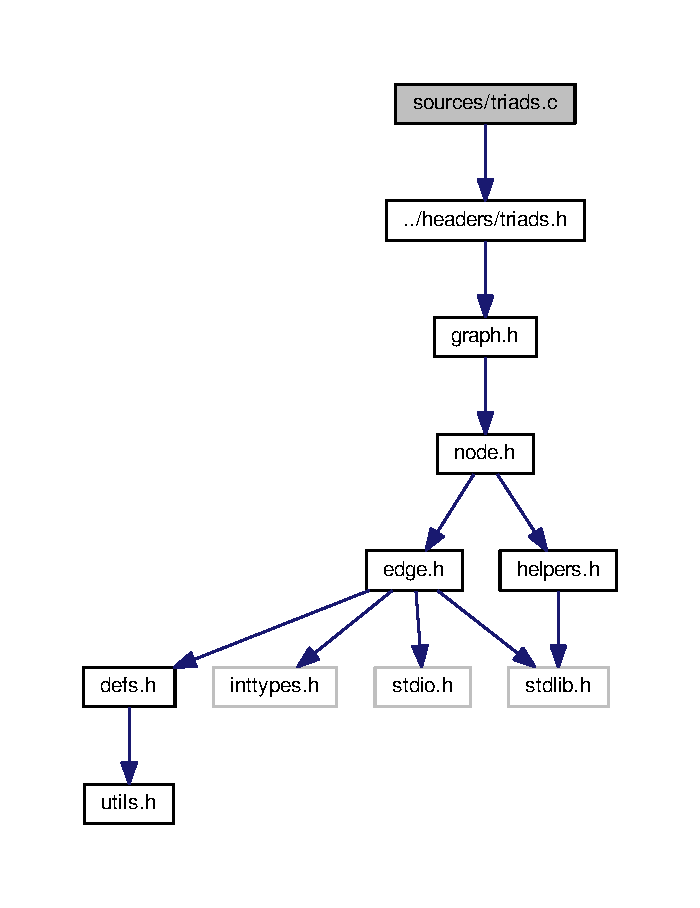
\includegraphics[width=336pt]{triads_8c__incl}
\end{center}
\end{figure}
\subsection*{Functions}
\begin{DoxyCompactItemize}
\item 
uint64\+\_\+t $\ast$ \hyperlink{triads_8c_a33470219fe7e4ce1cf0e82ac26332b54}{triad\+\_\+census\+\_\+\+BF} (\hyperlink{structGRAPH}{G\+R\+A\+PH} $\ast$g)
\begin{DoxyCompactList}\small\item\em Function that implements the Brute Force version of the triad census algorithm. \end{DoxyCompactList}\item 
uint64\+\_\+t $\ast$ \hyperlink{triads_8c_a5a46cb68a0606e745017030524e45098}{triad\+\_\+census\+\_\+\+BM} (\hyperlink{structGRAPH}{G\+R\+A\+PH} $\ast$g)
\begin{DoxyCompactList}\small\item\em Function that implements the Batagelj and Mrvar\textquotesingle{}s version of the triad census algorithm. \end{DoxyCompactList}\item 
void \hyperlink{triads_8c_a1bd1905d86d16197b1549c6d41d53b7f}{print\+\_\+triad\+\_\+census} (uint64\+\_\+t $\ast$triads)
\begin{DoxyCompactList}\small\item\em Function that prints the triad census. \end{DoxyCompactList}\item 
const char $\ast$ \hyperlink{triads_8c_ad1c0b7566793ee176e8ac06caf18d238}{return\+\_\+code} (int $\ast$triads)
\begin{DoxyCompactList}\small\item\em Function returns the code of a triad (for testing purposes) \end{DoxyCompactList}\item 
int \hyperlink{triads_8c_aba89c0fb106399c0731b4cfbcd0e743e}{iso\+Tricode} (\hyperlink{structNODE}{N\+O\+DE} $\ast$u, \hyperlink{structNODE}{N\+O\+DE} $\ast$v, \hyperlink{structNODE}{N\+O\+DE} $\ast$w)
\begin{DoxyCompactList}\small\item\em Function that computes the triad type of a triple of nodes. \end{DoxyCompactList}\item 
uint64\+\_\+t \hyperlink{triads_8c_af9d36341671cf11b24be96d4d1228181}{num\+\_\+total\+\_\+triads} (uint32\+\_\+t n)
\begin{DoxyCompactList}\small\item\em Function that computes and returns the number of triads present in a graph of n nodes. \end{DoxyCompactList}\end{DoxyCompactItemize}
\subsection*{Variables}
\begin{DoxyCompactItemize}
\item 
\hyperlink{utils_8h_a3e5b8192e7d9ffaf3542f1210aec18dd}{B\+O\+OL} \hyperlink{triads_8c_aa94b0ac5dc0f8919227cda71fe50db38}{ordered}
\item 
const char $\ast$ \hyperlink{triads_8c_a0f89b54966792be00877b79036adb727}{triad\+\_\+codes} \mbox{[}\hyperlink{utils_8h_ab2bde72626290c6daf5da1e9517aa8fb}{N\+U\+M\+\_\+\+T\+R\+I\+A\+DS}\mbox{]} = \{\char`\"{}003\char`\"{},\char`\"{}012\char`\"{},\char`\"{}102\char`\"{},\char`\"{}021\+D\char`\"{},\char`\"{}021\+U\char`\"{},\char`\"{}021\+C\char`\"{},\char`\"{}111\+D\char`\"{},\char`\"{}111\+U\char`\"{},\char`\"{}030\+T\char`\"{},\char`\"{}030\+C\char`\"{},\char`\"{}201\char`\"{},\char`\"{}120\+D\char`\"{},\char`\"{}120\+U\char`\"{},\char`\"{}120\+C\char`\"{},\char`\"{}210\char`\"{},\char`\"{}300\char`\"{}\}
\end{DoxyCompactItemize}


\subsection{Detailed Description}
This file contains the code that implements the functions defined in the header file \hyperlink{triads_8h}{triads.\+h}. Please refer to it to check the documentation. 

\begin{DoxyAuthor}{Author}
\+: Carlos Alfaro
\end{DoxyAuthor}
\begin{DoxyDate}{Date}
\+: 23-\/10-\/2017 
\end{DoxyDate}


\subsection{Function Documentation}
\mbox{\Hypertarget{triads_8c_aba89c0fb106399c0731b4cfbcd0e743e}\label{triads_8c_aba89c0fb106399c0731b4cfbcd0e743e}} 
\index{triads.\+c@{triads.\+c}!iso\+Tricode@{iso\+Tricode}}
\index{iso\+Tricode@{iso\+Tricode}!triads.\+c@{triads.\+c}}
\subsubsection{\texorpdfstring{iso\+Tricode()}{isoTricode()}}
{\footnotesize\ttfamily int iso\+Tricode (\begin{DoxyParamCaption}\item[{\hyperlink{structNODE}{N\+O\+DE} $\ast$}]{u,  }\item[{\hyperlink{structNODE}{N\+O\+DE} $\ast$}]{v,  }\item[{\hyperlink{structNODE}{N\+O\+DE} $\ast$}]{w }\end{DoxyParamCaption})}



Function that computes the triad type of a triple of nodes. 


\begin{DoxyParams}{Parameters}
{\em N\+O\+D\+E$\ast$} & u\+: First node of the triple \\
\hline
{\em N\+O\+D\+E$\ast$} & v\+: Second node of the triple \\
\hline
{\em N\+O\+D\+E$\ast$} & w\+: Third node of the triple\\
\hline
\end{DoxyParams}
\begin{DoxyReturn}{Returns}
int\+: A number between 0 and 15, depending on the configuration of the triple 
\end{DoxyReturn}
\mbox{\Hypertarget{triads_8c_af9d36341671cf11b24be96d4d1228181}\label{triads_8c_af9d36341671cf11b24be96d4d1228181}} 
\index{triads.\+c@{triads.\+c}!num\+\_\+total\+\_\+triads@{num\+\_\+total\+\_\+triads}}
\index{num\+\_\+total\+\_\+triads@{num\+\_\+total\+\_\+triads}!triads.\+c@{triads.\+c}}
\subsubsection{\texorpdfstring{num\+\_\+total\+\_\+triads()}{num\_total\_triads()}}
{\footnotesize\ttfamily uint64\+\_\+t num\+\_\+total\+\_\+triads (\begin{DoxyParamCaption}\item[{uint32\+\_\+t}]{n }\end{DoxyParamCaption})}



Function that computes and returns the number of triads present in a graph of n nodes. 


\begin{DoxyParams}{Parameters}
{\em uint32\+\_\+t} & n\+: The number of nodes of a graph\\
\hline
\end{DoxyParams}
\begin{DoxyReturn}{Returns}
uint32\+\_\+t\+: The number of total triads 
\end{DoxyReturn}
\mbox{\Hypertarget{triads_8c_a1bd1905d86d16197b1549c6d41d53b7f}\label{triads_8c_a1bd1905d86d16197b1549c6d41d53b7f}} 
\index{triads.\+c@{triads.\+c}!print\+\_\+triad\+\_\+census@{print\+\_\+triad\+\_\+census}}
\index{print\+\_\+triad\+\_\+census@{print\+\_\+triad\+\_\+census}!triads.\+c@{triads.\+c}}
\subsubsection{\texorpdfstring{print\+\_\+triad\+\_\+census()}{print\_triad\_census()}}
{\footnotesize\ttfamily void print\+\_\+triad\+\_\+census (\begin{DoxyParamCaption}\item[{uint64\+\_\+t $\ast$}]{triads }\end{DoxyParamCaption})}



Function that prints the triad census. 


\begin{DoxyParams}{Parameters}
{\em int$\ast$} & census\+: The vector containing the triad census\\
\hline
\end{DoxyParams}
\begin{DoxyReturn}{Returns}
None 
\end{DoxyReturn}
\mbox{\Hypertarget{triads_8c_ad1c0b7566793ee176e8ac06caf18d238}\label{triads_8c_ad1c0b7566793ee176e8ac06caf18d238}} 
\index{triads.\+c@{triads.\+c}!return\+\_\+code@{return\+\_\+code}}
\index{return\+\_\+code@{return\+\_\+code}!triads.\+c@{triads.\+c}}
\subsubsection{\texorpdfstring{return\+\_\+code()}{return\_code()}}
{\footnotesize\ttfamily const char$\ast$ return\+\_\+code (\begin{DoxyParamCaption}\item[{int $\ast$}]{census }\end{DoxyParamCaption})}



Function returns the code of a triad (for testing purposes) 


\begin{DoxyParams}{Parameters}
{\em int$\ast$} & census\+: The vector containing the triad census\\
\hline
\end{DoxyParams}
\begin{DoxyReturn}{Returns}
const char$\ast$\+: The triad code 
\end{DoxyReturn}
\mbox{\Hypertarget{triads_8c_a33470219fe7e4ce1cf0e82ac26332b54}\label{triads_8c_a33470219fe7e4ce1cf0e82ac26332b54}} 
\index{triads.\+c@{triads.\+c}!triad\+\_\+census\+\_\+\+BF@{triad\+\_\+census\+\_\+\+BF}}
\index{triad\+\_\+census\+\_\+\+BF@{triad\+\_\+census\+\_\+\+BF}!triads.\+c@{triads.\+c}}
\subsubsection{\texorpdfstring{triad\+\_\+census\+\_\+\+B\+F()}{triad\_census\_BF()}}
{\footnotesize\ttfamily uint64\+\_\+t$\ast$ triad\+\_\+census\+\_\+\+BF (\begin{DoxyParamCaption}\item[{\hyperlink{structGRAPH}{G\+R\+A\+PH} $\ast$}]{g }\end{DoxyParamCaption})}



Function that implements the Brute Force version of the triad census algorithm. 


\begin{DoxyParams}{Parameters}
{\em G\+R\+A\+P\+H$\ast$} & g\+: Pointer to the graph of which we want to perform the triad census\\
\hline
\end{DoxyParams}
\begin{DoxyReturn}{Returns}
int$\ast$\+: a vector containing the triad counts 
\end{DoxyReturn}
\mbox{\Hypertarget{triads_8c_a5a46cb68a0606e745017030524e45098}\label{triads_8c_a5a46cb68a0606e745017030524e45098}} 
\index{triads.\+c@{triads.\+c}!triad\+\_\+census\+\_\+\+BM@{triad\+\_\+census\+\_\+\+BM}}
\index{triad\+\_\+census\+\_\+\+BM@{triad\+\_\+census\+\_\+\+BM}!triads.\+c@{triads.\+c}}
\subsubsection{\texorpdfstring{triad\+\_\+census\+\_\+\+B\+M()}{triad\_census\_BM()}}
{\footnotesize\ttfamily uint64\+\_\+t$\ast$ triad\+\_\+census\+\_\+\+BM (\begin{DoxyParamCaption}\item[{\hyperlink{structGRAPH}{G\+R\+A\+PH} $\ast$}]{g }\end{DoxyParamCaption})}



Function that implements the Batagelj and Mrvar\textquotesingle{}s version of the triad census algorithm. 


\begin{DoxyParams}{Parameters}
{\em G\+R\+A\+P\+H$\ast$} & g\+: Pointer to the graph of which we want to perform the triad census\\
\hline
\end{DoxyParams}
\begin{DoxyReturn}{Returns}
int$\ast$\+: a vector containing the triad counts 
\end{DoxyReturn}


\subsection{Variable Documentation}
\mbox{\Hypertarget{triads_8c_aa94b0ac5dc0f8919227cda71fe50db38}\label{triads_8c_aa94b0ac5dc0f8919227cda71fe50db38}} 
\index{triads.\+c@{triads.\+c}!ordered@{ordered}}
\index{ordered@{ordered}!triads.\+c@{triads.\+c}}
\subsubsection{\texorpdfstring{ordered}{ordered}}
{\footnotesize\ttfamily \hyperlink{utils_8h_a3e5b8192e7d9ffaf3542f1210aec18dd}{B\+O\+OL} ordered}

Flag to determine whether the data managed has to be ordered or not \mbox{\Hypertarget{triads_8c_a0f89b54966792be00877b79036adb727}\label{triads_8c_a0f89b54966792be00877b79036adb727}} 
\index{triads.\+c@{triads.\+c}!triad\+\_\+codes@{triad\+\_\+codes}}
\index{triad\+\_\+codes@{triad\+\_\+codes}!triads.\+c@{triads.\+c}}
\subsubsection{\texorpdfstring{triad\+\_\+codes}{triad\_codes}}
{\footnotesize\ttfamily const char$\ast$ triad\+\_\+codes\mbox{[}\hyperlink{utils_8h_ab2bde72626290c6daf5da1e9517aa8fb}{N\+U\+M\+\_\+\+T\+R\+I\+A\+DS}\mbox{]} = \{\char`\"{}003\char`\"{},\char`\"{}012\char`\"{},\char`\"{}102\char`\"{},\char`\"{}021\+D\char`\"{},\char`\"{}021\+U\char`\"{},\char`\"{}021\+C\char`\"{},\char`\"{}111\+D\char`\"{},\char`\"{}111\+U\char`\"{},\char`\"{}030\+T\char`\"{},\char`\"{}030\+C\char`\"{},\char`\"{}201\char`\"{},\char`\"{}120\+D\char`\"{},\char`\"{}120\+U\char`\"{},\char`\"{}120\+C\char`\"{},\char`\"{}210\char`\"{},\char`\"{}300\char`\"{}\}}

Triad codes 
%--- End generated contents ---

% Index
\backmatter
\newpage
\phantomsection
\clearemptydoublepage
\addcontentsline{toc}{chapter}{Index}
\printindex

\end{document}
